\documentclass[11pt,a4paper]{book}
\usepackage[vmargin=3cm,rmargin=3cm,lmargin=3cm]{geometry}
\setlength\parindent{0pt}

\usepackage{appendix}

\usepackage{parskip}
\usepackage{paralist}

\usepackage[round]{natbib}
\bibliography{refs}

% \renewcommand{\chaptername}{Module}
\usepackage{gensymb}
\usepackage[T1]{fontenc}
\usepackage{mathptmx}
\usepackage{helvet}
\usepackage{courier}
\usepackage{amsmath}
% \usepackage[fleqn]{amsmath}
\usepackage{amssymb}
\usepackage{pdfpages}

\usepackage{framed} % For snugshade boxes
\usepackage{sectsty}
\usepackage{multicol} % used for the two-column index

% \setlength{\intextsep}{0pt} %to reduce top and bottom spacing in wrapfigs
\usepackage{wrapfig}
\usepackage{graphicx}        % standard LaTeX graphics tool
\graphicspath{{Graphics/}}
\usepackage{float} %to override default float behavior of figures 

% \usepackage[bottom]{footmisc}% places footnotes at page bottom
\usepackage{tikz}
\usetikzlibrary{positioning, fit}
\usepackage{hyperref}
\hypersetup{%
  colorlinks=false,% hyperlinks will be black
  linkbordercolor=white,% hyperlink borders will be invisibless
  pdfborderstyle={/S/U/W 1}% border style will be underline of width 1pt
}

\usepackage{color}
\usepackage{textcomp}
\usepackage{setspace}
\usepackage{verbatim}

\renewcommand{\arraystretch}{1.3} %spacing between table rows

\sloppy
%%%%%%%%%%%%%%%%%%%%%%%%%%%%%%%%%%%%%%%%%%%%%%%%%%%%%%%%%%%%%%%%%%%%
\usepackage[many]{tcolorbox} %for the tip boxes
\newtcolorbox{tipbox}{
breakable,
freelance,
colback=white,
frame code={},
overlay unbroken={
  \fill[rounded corners=8pt,gray!30]
    (title.south west) --
    (title.south) -- 
    ([yshift=20pt]title.south) --
    ([yshift=20pt,xshift=4cm]title.south) --
    ([xshift=4cm]title.south) --
    (title.south east) {[sharp corners] --
    ([yshift=-6pt]title.south east) -- 
    ([yshift=-6pt]title.south west) } -- cycle;
  \draw[rounded corners=8pt,gray,line width=1pt]
    (title.west|-frame.south west) --
    (title.south west) --
    (title.south) -- 
    ([yshift=20pt]title.south) --
    ([yshift=20pt,xshift=4cm]title.south) --
    ([xshift=4cm]title.south) --
    (title.south east) --
    (title.east|-frame.south east) --
    cycle;
  \node at ([xshift=2cm,yshift=4pt,font=]title.south) 
    {\sffamily\Large Tip~\thetcbcounter};  
    }, 
overlay first={
  \fill[rounded corners=8pt,gray!30]
    (title.south west) --
    (title.south) -- 
    ([yshift=20pt]title.south) --
    ([yshift=20pt,xshift=4cm]title.south) --
    ([xshift=4cm]title.south) --
    (title.south east) {[sharp corners] --
    ([yshift=-6pt]title.south east) -- 
    ([yshift=-6pt]title.south west) } -- cycle;
    \draw[rounded corners=8pt,gray,line width=1pt]
    (title.west|-frame.south) --
    (title.south west) --
    (title.south) -- 
    ([yshift=20pt]title.south) --
    ([yshift=20pt,xshift=4cm]title.south) --
    ([xshift=4cm]title.south) --
    (title.south east) --
    (title.south east|-frame.south);
  \node at ([xshift=2cm,yshift=4pt,font=]title.south) 
    {\sffamily\Large Tip~\thetcbcounter};  
  },
overlay middle={
  \draw[rounded corners=8pt,gray,line width=1pt]
    (title.west|-frame.south) --
    (title.west|-frame.north);
  \draw[rounded corners=8pt,gray,line width=1pt]
    (title.east|-frame.south) --
    (title.east|-frame.north);
  },
overlay last={
  \draw[rounded corners=8pt,gray,line width=1pt]
    (title.west|-frame.north) --
    (title.west|-frame.south) --
    (title.east|-frame.south) --
    (title.east|-frame.north);
  },
title={\mbox{}},
% top=12pt,
fontupper=\bf,
% oversize=0.5cm,
before={\vskip28pt\par\noindent},
after={\par\vskip12pt},
}
%%%%%%%%%%%%%%%%%%%%%%%%%%%%%%%%%%%%%%%%%%%%%%%%%%%%%%%%%%%%%%%%%%%%

\usepackage [autostyle]{csquotes}
\MakeOuterQuote{"}

\usepackage{epigraph}


% \definecolor{AliceBlue}{rgb}{0.94,0.97,1.00}
\definecolor{AntiqueWhite1}{rgb}{1.00,0.94,0.86}
\definecolor{AntiqueWhite2}{rgb}{0.93,0.87,0.80}
\definecolor{AntiqueWhite3}{rgb}{0.80,0.75,0.69}
\definecolor{AntiqueWhite4}{rgb}{0.55,0.51,0.47}
\definecolor{AntiqueWhite}{rgb}{0.98,0.92,0.84}
\definecolor{BlanchedAlmond}{rgb}{1.00,0.92,0.80}
\definecolor{BlueViolet}{rgb}{0.54,0.17,0.89}
\definecolor{CadetBlue1}{rgb}{0.60,0.96,1.00}
\definecolor{CadetBlue2}{rgb}{0.56,0.90,0.93}
\definecolor{CadetBlue3}{rgb}{0.48,0.77,0.80}
\definecolor{CadetBlue4}{rgb}{0.33,0.53,0.55}
\definecolor{CadetBlue}{rgb}{0.37,0.62,0.63}
\definecolor{CornflowerBlue}{rgb}{0.39,0.58,0.93}
\definecolor{DarkBlue}{rgb}{0.00,0.00,0.55}
\definecolor{DarkCyan}{rgb}{0.00,0.55,0.55}
\definecolor{DarkGoldenrod1}{rgb}{1.00,0.73,0.06}
\definecolor{DarkGoldenrod2}{rgb}{0.93,0.68,0.05}
\definecolor{DarkGoldenrod3}{rgb}{0.80,0.58,0.05}
\definecolor{DarkGoldenrod4}{rgb}{0.55,0.40,0.03}
\definecolor{DarkGoldenrod}{rgb}{0.72,0.53,0.04}
\definecolor{DarkGray}{rgb}{0.66,0.66,0.66}
\definecolor{DarkGreen}{rgb}{0.00,0.39,0.00}
\definecolor{DarkGrey}{rgb}{0.66,0.66,0.66}
\definecolor{DarkKhaki}{rgb}{0.74,0.72,0.42}
\definecolor{DarkMagenta}{rgb}{0.55,0.00,0.55}
\definecolor{DarkOliveGreen1}{rgb}{0.79,1.00,0.44}
\definecolor{DarkOliveGreen2}{rgb}{0.74,0.93,0.41}
\definecolor{DarkOliveGreen3}{rgb}{0.64,0.80,0.35}
\definecolor{DarkOliveGreen4}{rgb}{0.43,0.55,0.24}
\definecolor{DarkOliveGreen}{rgb}{0.33,0.42,0.18}
\definecolor{DarkOrange1}{rgb}{1.00,0.50,0.00}
\definecolor{DarkOrange2}{rgb}{0.93,0.46,0.00}
\definecolor{DarkOrange3}{rgb}{0.80,0.40,0.00}
\definecolor{DarkOrange4}{rgb}{0.55,0.27,0.00}
\definecolor{DarkOrange}{rgb}{1.00,0.55,0.00}
\definecolor{DarkOrchid1}{rgb}{0.75,0.24,1.00}
\definecolor{DarkOrchid2}{rgb}{0.70,0.23,0.93}
\definecolor{DarkOrchid3}{rgb}{0.60,0.20,0.80}
\definecolor{DarkOrchid4}{rgb}{0.41,0.13,0.55}
\definecolor{DarkOrchid}{rgb}{0.60,0.20,0.80}
\definecolor{DarkRed}{rgb}{0.55,0.00,0.00}
\definecolor{DarkSalmon}{rgb}{0.91,0.59,0.48}
\definecolor{DarkSeaGreen1}{rgb}{0.76,1.00,0.76}
\definecolor{DarkSeaGreen2}{rgb}{0.71,0.93,0.71}
\definecolor{DarkSeaGreen3}{rgb}{0.61,0.80,0.61}
\definecolor{DarkSeaGreen4}{rgb}{0.41,0.55,0.41}
\definecolor{DarkSeaGreen}{rgb}{0.56,0.74,0.56}
\definecolor{DarkSlateBlue}{rgb}{0.28,0.24,0.55}
\definecolor{DarkSlateGray1}{rgb}{0.59,1.00,1.00}
\definecolor{DarkSlateGray2}{rgb}{0.55,0.93,0.93}
\definecolor{DarkSlateGray3}{rgb}{0.47,0.80,0.80}
\definecolor{DarkSlateGray4}{rgb}{0.32,0.55,0.55}
\definecolor{DarkSlateGray}{rgb}{0.18,0.31,0.31}
\definecolor{DarkSlateGrey}{rgb}{0.18,0.31,0.31}
\definecolor{DarkTurquoise}{rgb}{0.00,0.81,0.82}
\definecolor{DarkViolet}{rgb}{0.58,0.00,0.83}
\definecolor{DeepPink1}{rgb}{1.00,0.08,0.58}
\definecolor{DeepPink2}{rgb}{0.93,0.07,0.54}
\definecolor{DeepPink3}{rgb}{0.80,0.06,0.46}
\definecolor{DeepPink4}{rgb}{0.55,0.04,0.31}
\definecolor{DeepPink}{rgb}{1.00,0.08,0.58}
\definecolor{DeepSkyBlue1}{rgb}{0.00,0.75,1.00}
\definecolor{DeepSkyBlue2}{rgb}{0.00,0.70,0.93}
\definecolor{DeepSkyBlue3}{rgb}{0.00,0.60,0.80}
\definecolor{DeepSkyBlue4}{rgb}{0.00,0.41,0.55}
\definecolor{DeepSkyBlue}{rgb}{0.00,0.75,1.00}
\definecolor{DimGray}{rgb}{0.41,0.41,0.41}
\definecolor{DimGrey}{rgb}{0.41,0.41,0.41}
\definecolor{DodgerBlue1}{rgb}{0.12,0.56,1.00}
\definecolor{DodgerBlue2}{rgb}{0.11,0.53,0.93}
\definecolor{DodgerBlue3}{rgb}{0.09,0.45,0.80}
\definecolor{DodgerBlue4}{rgb}{0.06,0.31,0.55}
\definecolor{DodgerBlue}{rgb}{0.12,0.56,1.00}
\definecolor{FloralWhite}{rgb}{1.00,0.98,0.94}
\definecolor{ForestGreen}{rgb}{0.13,0.55,0.13}
\definecolor{GhostWhite}{rgb}{0.97,0.97,1.00}
\definecolor{GreenYellow}{rgb}{0.68,1.00,0.18}
\definecolor{HotPink1}{rgb}{1.00,0.43,0.71}
\definecolor{HotPink2}{rgb}{0.93,0.42,0.65}
\definecolor{HotPink3}{rgb}{0.80,0.38,0.56}
\definecolor{HotPink4}{rgb}{0.55,0.23,0.38}
\definecolor{HotPink}{rgb}{1.00,0.41,0.71}
\definecolor{IndianRed1}{rgb}{1.00,0.42,0.42}
\definecolor{IndianRed2}{rgb}{0.93,0.39,0.39}
\definecolor{IndianRed3}{rgb}{0.80,0.33,0.33}
\definecolor{IndianRed4}{rgb}{0.55,0.23,0.23}
\definecolor{IndianRed}{rgb}{0.80,0.36,0.36}
\definecolor{LavenderBlush1}{rgb}{1.00,0.94,0.96}
\definecolor{LavenderBlush2}{rgb}{0.93,0.88,0.90}
\definecolor{LavenderBlush3}{rgb}{0.80,0.76,0.77}
\definecolor{LavenderBlush4}{rgb}{0.55,0.51,0.53}
\definecolor{LavenderBlush}{rgb}{1.00,0.94,0.96}
\definecolor{LawnGreen}{rgb}{0.49,0.99,0.00}
\definecolor{LemonChiffon1}{rgb}{1.00,0.98,0.80}
\definecolor{LemonChiffon2}{rgb}{0.93,0.91,0.75}
\definecolor{LemonChiffon3}{rgb}{0.80,0.79,0.65}
\definecolor{LemonChiffon4}{rgb}{0.55,0.54,0.44}
\definecolor{LemonChiffon}{rgb}{1.00,0.98,0.80}
\definecolor{LightBlue1}{rgb}{0.75,0.94,1.00}
\definecolor{LightBlue2}{rgb}{0.70,0.87,0.93}
\definecolor{LightBlue3}{rgb}{0.60,0.75,0.80}
\definecolor{LightBlue4}{rgb}{0.41,0.51,0.55}
\definecolor{LightBlue}{rgb}{0.68,0.85,0.90}
\definecolor{LightCoral}{rgb}{0.94,0.50,0.50}
\definecolor{LightCyan1}{rgb}{0.88,1.00,1.00}
\definecolor{LightCyan2}{rgb}{0.82,0.93,0.93}
\definecolor{LightCyan3}{rgb}{0.71,0.80,0.80}
\definecolor{LightCyan4}{rgb}{0.48,0.55,0.55}
\definecolor{LightCyan}{rgb}{0.88,1.00,1.00}
\definecolor{LightGoldenrod1}{rgb}{1.00,0.93,0.55}
\definecolor{LightGoldenrod2}{rgb}{0.93,0.86,0.51}
\definecolor{LightGoldenrod3}{rgb}{0.80,0.75,0.44}
\definecolor{LightGoldenrod4}{rgb}{0.55,0.51,0.30}
\definecolor{LightGoldenrodYellow}{rgb}{0.98,0.98,0.82}
\definecolor{LightGoldenrod}{rgb}{0.93,0.87,0.51}
\definecolor{LightGray}{rgb}{0.83,0.83,0.83}
\definecolor{LightGreen}{rgb}{0.56,0.93,0.56}
\definecolor{LightGrey}{rgb}{0.83,0.83,0.83}
\definecolor{LightPink1}{rgb}{1.00,0.68,0.73}
\definecolor{LightPink2}{rgb}{0.93,0.64,0.68}
\definecolor{LightPink3}{rgb}{0.80,0.55,0.58}
\definecolor{LightPink4}{rgb}{0.55,0.37,0.40}
\definecolor{LightPink}{rgb}{1.00,0.71,0.76}
\definecolor{LightSalmon1}{rgb}{1.00,0.63,0.48}
\definecolor{LightSalmon2}{rgb}{0.93,0.58,0.45}
\definecolor{LightSalmon3}{rgb}{0.80,0.51,0.38}
\definecolor{LightSalmon4}{rgb}{0.55,0.34,0.26}
\definecolor{LightSalmon}{rgb}{1.00,0.63,0.48}
\definecolor{LightSeaGreen}{rgb}{0.13,0.70,0.67}
\definecolor{LightSkyBlue1}{rgb}{0.69,0.89,1.00}
\definecolor{LightSkyBlue2}{rgb}{0.64,0.83,0.93}
\definecolor{LightSkyBlue3}{rgb}{0.55,0.71,0.80}
\definecolor{LightSkyBlue4}{rgb}{0.38,0.48,0.55}
\definecolor{LightSkyBlue}{rgb}{0.53,0.81,0.98}
\definecolor{LightSlateBlue}{rgb}{0.52,0.44,1.00}
\definecolor{LightSlateGray}{rgb}{0.47,0.53,0.60}
\definecolor{LightSlateGrey}{rgb}{0.47,0.53,0.60}
\definecolor{LightSteelBlue1}{rgb}{0.79,0.88,1.00}
\definecolor{LightSteelBlue2}{rgb}{0.74,0.82,0.93}
\definecolor{LightSteelBlue3}{rgb}{0.64,0.71,0.80}
\definecolor{LightSteelBlue4}{rgb}{0.43,0.48,0.55}
\definecolor{LightSteelBlue}{rgb}{0.69,0.77,0.87}
\definecolor{LightYellow1}{rgb}{1.00,1.00,0.88}
\definecolor{LightYellow2}{rgb}{0.93,0.93,0.82}
\definecolor{LightYellow3}{rgb}{0.80,0.80,0.71}
\definecolor{LightYellow4}{rgb}{0.55,0.55,0.48}
\definecolor{LightYellow}{rgb}{1.00,1.00,0.88}
\definecolor{LimeGreen}{rgb}{0.20,0.80,0.20}
\definecolor{MediumAquamarine}{rgb}{0.40,0.80,0.67}
\definecolor{MediumBlue}{rgb}{0.00,0.00,0.80}
\definecolor{MediumOrchid1}{rgb}{0.88,0.40,1.00}
\definecolor{MediumOrchid2}{rgb}{0.82,0.37,0.93}
\definecolor{MediumOrchid3}{rgb}{0.71,0.32,0.80}
\definecolor{MediumOrchid4}{rgb}{0.48,0.22,0.55}
\definecolor{MediumOrchid}{rgb}{0.73,0.33,0.83}
\definecolor{MediumPurple1}{rgb}{0.67,0.51,1.00}
\definecolor{MediumPurple2}{rgb}{0.62,0.47,0.93}
\definecolor{MediumPurple3}{rgb}{0.54,0.41,0.80}
\definecolor{MediumPurple4}{rgb}{0.36,0.28,0.55}
\definecolor{MediumPurple}{rgb}{0.58,0.44,0.86}
\definecolor{MediumSeaGreen}{rgb}{0.24,0.70,0.44}
\definecolor{MediumSlateBlue}{rgb}{0.48,0.41,0.93}
\definecolor{MediumSpringGreen}{rgb}{0.00,0.98,0.60}
\definecolor{MediumTurquoise}{rgb}{0.28,0.82,0.80}
\definecolor{MediumVioletRed}{rgb}{0.78,0.08,0.52}
\definecolor{MidnightBlue}{rgb}{0.10,0.10,0.44}
\definecolor{MintCream}{rgb}{0.96,1.00,0.98}
\definecolor{MistyRose1}{rgb}{1.00,0.89,0.88}
\definecolor{MistyRose2}{rgb}{0.93,0.84,0.82}
\definecolor{MistyRose3}{rgb}{0.80,0.72,0.71}
\definecolor{MistyRose4}{rgb}{0.55,0.49,0.48}
\definecolor{MistyRose}{rgb}{1.00,0.89,0.88}
\definecolor{NavajoWhite1}{rgb}{1.00,0.87,0.68}
\definecolor{NavajoWhite2}{rgb}{0.93,0.81,0.63}
\definecolor{NavajoWhite3}{rgb}{0.80,0.70,0.55}
\definecolor{NavajoWhite4}{rgb}{0.55,0.47,0.37}
\definecolor{NavajoWhite}{rgb}{1.00,0.87,0.68}
\definecolor{NavyBlue}{rgb}{0.00,0.00,0.50}
\definecolor{OldLace}{rgb}{0.99,0.96,0.90}
\definecolor{OliveDrab1}{rgb}{0.75,1.00,0.24}
\definecolor{OliveDrab2}{rgb}{0.70,0.93,0.23}
\definecolor{OliveDrab3}{rgb}{0.60,0.80,0.20}
\definecolor{OliveDrab4}{rgb}{0.41,0.55,0.13}
\definecolor{OliveDrab}{rgb}{0.42,0.56,0.14}
\definecolor{OrangeRed1}{rgb}{1.00,0.27,0.00}
\definecolor{OrangeRed2}{rgb}{0.93,0.25,0.00}
\definecolor{OrangeRed3}{rgb}{0.80,0.22,0.00}
\definecolor{OrangeRed4}{rgb}{0.55,0.15,0.00}
\definecolor{OrangeRed}{rgb}{1.00,0.27,0.00}
\definecolor{PaleGoldenrod}{rgb}{0.93,0.91,0.67}
\definecolor{PaleGreen1}{rgb}{0.60,1.00,0.60}
\definecolor{PaleGreen2}{rgb}{0.56,0.93,0.56}
\definecolor{PaleGreen3}{rgb}{0.49,0.80,0.49}
\definecolor{PaleGreen4}{rgb}{0.33,0.55,0.33}
\definecolor{PaleGreen}{rgb}{0.60,0.98,0.60}
\definecolor{PaleTurquoise1}{rgb}{0.73,1.00,1.00}
\definecolor{PaleTurquoise2}{rgb}{0.68,0.93,0.93}
\definecolor{PaleTurquoise3}{rgb}{0.59,0.80,0.80}
\definecolor{PaleTurquoise4}{rgb}{0.40,0.55,0.55}
\definecolor{PaleTurquoise}{rgb}{0.69,0.93,0.93}
\definecolor{PaleVioletRed1}{rgb}{1.00,0.51,0.67}
\definecolor{PaleVioletRed2}{rgb}{0.93,0.47,0.62}
\definecolor{PaleVioletRed3}{rgb}{0.80,0.41,0.54}
\definecolor{PaleVioletRed4}{rgb}{0.55,0.28,0.36}
\definecolor{PaleVioletRed}{rgb}{0.86,0.44,0.58}
\definecolor{PapayaWhip}{rgb}{1.00,0.94,0.84}
\definecolor{PeachPuff1}{rgb}{1.00,0.85,0.73}
\definecolor{PeachPuff2}{rgb}{0.93,0.80,0.68}
\definecolor{PeachPuff3}{rgb}{0.80,0.69,0.58}
\definecolor{PeachPuff4}{rgb}{0.55,0.47,0.40}
\definecolor{PeachPuff}{rgb}{1.00,0.85,0.73}
\definecolor{PowderBlue}{rgb}{0.69,0.88,0.90}
\definecolor{RosyBrown1}{rgb}{1.00,0.76,0.76}
\definecolor{RosyBrown2}{rgb}{0.93,0.71,0.71}
\definecolor{RosyBrown3}{rgb}{0.80,0.61,0.61}
\definecolor{RosyBrown4}{rgb}{0.55,0.41,0.41}
\definecolor{RosyBrown}{rgb}{0.74,0.56,0.56}
\definecolor{RoyalBlue1}{rgb}{0.28,0.46,1.00}
\definecolor{RoyalBlue2}{rgb}{0.26,0.43,0.93}
\definecolor{RoyalBlue3}{rgb}{0.23,0.37,0.80}
\definecolor{RoyalBlue4}{rgb}{0.15,0.25,0.55}
\definecolor{RoyalBlue}{rgb}{0.25,0.41,0.88}
\definecolor{SaddleBrown}{rgb}{0.55,0.27,0.07}
\definecolor{SandyBrown}{rgb}{0.96,0.64,0.38}
\definecolor{SeaGreen1}{rgb}{0.33,1.00,0.62}
\definecolor{SeaGreen2}{rgb}{0.31,0.93,0.58}
\definecolor{SeaGreen3}{rgb}{0.26,0.80,0.50}
\definecolor{SeaGreen4}{rgb}{0.18,0.55,0.34}
\definecolor{SeaGreen}{rgb}{0.18,0.55,0.34}
\definecolor{SkyBlue1}{rgb}{0.53,0.81,1.00}
\definecolor{SkyBlue2}{rgb}{0.49,0.75,0.93}
\definecolor{SkyBlue3}{rgb}{0.42,0.65,0.80}
\definecolor{SkyBlue4}{rgb}{0.29,0.44,0.55}
\definecolor{SkyBlue}{rgb}{0.53,0.81,0.92}
\definecolor{SlateBlue1}{rgb}{0.51,0.44,1.00}
\definecolor{SlateBlue2}{rgb}{0.48,0.40,0.93}
\definecolor{SlateBlue3}{rgb}{0.41,0.35,0.80}
\definecolor{SlateBlue4}{rgb}{0.28,0.24,0.55}
\definecolor{SlateBlue}{rgb}{0.42,0.35,0.80}
\definecolor{SlateGray1}{rgb}{0.78,0.89,1.00}
\definecolor{SlateGray2}{rgb}{0.73,0.83,0.93}
\definecolor{SlateGray3}{rgb}{0.62,0.71,0.80}
\definecolor{SlateGray4}{rgb}{0.42,0.48,0.55}
\definecolor{SlateGray}{rgb}{0.44,0.50,0.56}
\definecolor{SlateGrey}{rgb}{0.44,0.50,0.56}
\definecolor{SpringGreen1}{rgb}{0.00,1.00,0.50}
\definecolor{SpringGreen2}{rgb}{0.00,0.93,0.46}
\definecolor{SpringGreen3}{rgb}{0.00,0.80,0.40}
\definecolor{SpringGreen4}{rgb}{0.00,0.55,0.27}
\definecolor{SpringGreen}{rgb}{0.00,1.00,0.50}
\definecolor{SteelBlue1}{rgb}{0.39,0.72,1.00}
\definecolor{SteelBlue2}{rgb}{0.36,0.67,0.93}
\definecolor{SteelBlue3}{rgb}{0.31,0.58,0.80}
\definecolor{SteelBlue4}{rgb}{0.21,0.39,0.55}
\definecolor{SteelBlue}{rgb}{0.27,0.51,0.71}
\definecolor{VioletRed1}{rgb}{1.00,0.24,0.59}
\definecolor{VioletRed2}{rgb}{0.93,0.23,0.55}
\definecolor{VioletRed3}{rgb}{0.80,0.20,0.47}
\definecolor{VioletRed4}{rgb}{0.55,0.13,0.32}
\definecolor{VioletRed}{rgb}{0.82,0.13,0.56}
\definecolor{WhiteSmoke}{rgb}{0.96,0.96,0.96}
\definecolor{YellowGreen}{rgb}{0.60,0.80,0.20}
\definecolor{aliceblue}{rgb}{0.94,0.97,1.00}
\definecolor{antiquewhite}{rgb}{0.98,0.92,0.84}
\definecolor{aquamarine1}{rgb}{0.50,1.00,0.83}
\definecolor{aquamarine2}{rgb}{0.46,0.93,0.78}
\definecolor{aquamarine3}{rgb}{0.40,0.80,0.67}
\definecolor{aquamarine4}{rgb}{0.27,0.55,0.45}
\definecolor{aquamarine}{rgb}{0.50,1.00,0.83}
\definecolor{azure1}{rgb}{0.94,1.00,1.00}
\definecolor{azure2}{rgb}{0.88,0.93,0.93}
\definecolor{azure3}{rgb}{0.76,0.80,0.80}
\definecolor{azure4}{rgb}{0.51,0.55,0.55}
\definecolor{azure}{rgb}{0.94,1.00,1.00}
\definecolor{beige}{rgb}{0.96,0.96,0.86}
\definecolor{bisque1}{rgb}{1.00,0.89,0.77}
\definecolor{bisque2}{rgb}{0.93,0.84,0.72}
\definecolor{bisque3}{rgb}{0.80,0.72,0.62}
\definecolor{bisque4}{rgb}{0.55,0.49,0.42}
\definecolor{bisque}{rgb}{1.00,0.89,0.77}
\definecolor{black}{rgb}{0.00,0.00,0.00}
\definecolor{blanchedalmond}{rgb}{1.00,0.92,0.80}
\definecolor{blue1}{rgb}{0.00,0.00,1.00}
\definecolor{blue2}{rgb}{0.00,0.00,0.93}
\definecolor{blue3}{rgb}{0.00,0.00,0.80}
\definecolor{blue4}{rgb}{0.00,0.00,0.55}
\definecolor{blueviolet}{rgb}{0.54,0.17,0.89}
\definecolor{blue}{rgb}{0.00,0.00,1.00}
\definecolor{brown1}{rgb}{1.00,0.25,0.25}
\definecolor{brown2}{rgb}{0.93,0.23,0.23}
\definecolor{brown3}{rgb}{0.80,0.20,0.20}
\definecolor{brown4}{rgb}{0.55,0.14,0.14}
\definecolor{brown}{rgb}{0.65,0.16,0.16}
\definecolor{burlywood1}{rgb}{1.00,0.83,0.61}
\definecolor{burlywood2}{rgb}{0.93,0.77,0.57}
\definecolor{burlywood3}{rgb}{0.80,0.67,0.49}
\definecolor{burlywood4}{rgb}{0.55,0.45,0.33}
\definecolor{burlywood}{rgb}{0.87,0.72,0.53}
\definecolor{cadetblue}{rgb}{0.37,0.62,0.63}
\definecolor{chartreuse1}{rgb}{0.50,1.00,0.00}
\definecolor{chartreuse2}{rgb}{0.46,0.93,0.00}
\definecolor{chartreuse3}{rgb}{0.40,0.80,0.00}
\definecolor{chartreuse4}{rgb}{0.27,0.55,0.00}
\definecolor{chartreuse}{rgb}{0.50,1.00,0.00}
\definecolor{chocolate1}{rgb}{1.00,0.50,0.14}
\definecolor{chocolate2}{rgb}{0.93,0.46,0.13}
\definecolor{chocolate3}{rgb}{0.80,0.40,0.11}
\definecolor{chocolate4}{rgb}{0.55,0.27,0.07}
\definecolor{chocolate}{rgb}{0.82,0.41,0.12}
\definecolor{coral1}{rgb}{1.00,0.45,0.34}
\definecolor{coral2}{rgb}{0.93,0.42,0.31}
\definecolor{coral3}{rgb}{0.80,0.36,0.27}
\definecolor{coral4}{rgb}{0.55,0.24,0.18}
\definecolor{coral}{rgb}{1.00,0.50,0.31}
\definecolor{cornflowerblue}{rgb}{0.39,0.58,0.93}
\definecolor{cornsilk1}{rgb}{1.00,0.97,0.86}
\definecolor{cornsilk2}{rgb}{0.93,0.91,0.80}
\definecolor{cornsilk3}{rgb}{0.80,0.78,0.69}
\definecolor{cornsilk4}{rgb}{0.55,0.53,0.47}
\definecolor{cornsilk}{rgb}{1.00,0.97,0.86}
\definecolor{cyan1}{rgb}{0.00,1.00,1.00}
\definecolor{cyan2}{rgb}{0.00,0.93,0.93}
\definecolor{cyan3}{rgb}{0.00,0.80,0.80}
\definecolor{cyan4}{rgb}{0.00,0.55,0.55}
\definecolor{cyan}{rgb}{0.00,1.00,1.00}
\definecolor{darkblue}{rgb}{0.00,0.00,0.55}
\definecolor{darkcyan}{rgb}{0.00,0.55,0.55}
\definecolor{darkgoldenrod}{rgb}{0.72,0.53,0.04}
\definecolor{darkgray}{rgb}{0.66,0.66,0.66}
\definecolor{darkgreen}{rgb}{0.00,0.39,0.00}
\definecolor{darkgrey}{rgb}{0.66,0.66,0.66}
\definecolor{darkkhaki}{rgb}{0.74,0.72,0.42}
\definecolor{darkmagenta}{rgb}{0.55,0.00,0.55}
\definecolor{darkolive}{rgb}{0.33,0.42,0.18}
\definecolor{darkorange}{rgb}{1.00,0.55,0.00}
\definecolor{darkorchid}{rgb}{0.60,0.20,0.80}
\definecolor{darkred}{rgb}{0.55,0.00,0.00}
\definecolor{darksalmon}{rgb}{0.91,0.59,0.48}
\definecolor{darksea}{rgb}{0.56,0.74,0.56}
\definecolor{darkslate}{rgb}{0.18,0.31,0.31}
\definecolor{darkslate}{rgb}{0.18,0.31,0.31}
\definecolor{darkslate}{rgb}{0.28,0.24,0.55}
\definecolor{darkturquoise}{rgb}{0.00,0.81,0.82}
\definecolor{darkviolet}{rgb}{0.58,0.00,0.83}
\definecolor{deeppink}{rgb}{1.00,0.08,0.58}
\definecolor{deepsky}{rgb}{0.00,0.75,1.00}
\definecolor{dimgray}{rgb}{0.41,0.41,0.41}
\definecolor{dimgrey}{rgb}{0.41,0.41,0.41}
\definecolor{dodgerblue}{rgb}{0.12,0.56,1.00}
\definecolor{firebrick1}{rgb}{1.00,0.19,0.19}
\definecolor{firebrick2}{rgb}{0.93,0.17,0.17}
\definecolor{firebrick3}{rgb}{0.80,0.15,0.15}
\definecolor{firebrick4}{rgb}{0.55,0.10,0.10}
\definecolor{firebrick}{rgb}{0.70,0.13,0.13}
\definecolor{floralwhite}{rgb}{1.00,0.98,0.94}
\definecolor{forestgreen}{rgb}{0.13,0.55,0.13}
\definecolor{gainsboro}{rgb}{0.86,0.86,0.86}
\definecolor{ghostwhite}{rgb}{0.97,0.97,1.00}
\definecolor{gold1}{rgb}{1.00,0.84,0.00}
\definecolor{gold2}{rgb}{0.93,0.79,0.00}
\definecolor{gold3}{rgb}{0.80,0.68,0.00}
\definecolor{gold4}{rgb}{0.55,0.46,0.00}
\definecolor{goldenrod1}{rgb}{1.00,0.76,0.15}
\definecolor{goldenrod2}{rgb}{0.93,0.71,0.13}
\definecolor{goldenrod3}{rgb}{0.80,0.61,0.11}
\definecolor{goldenrod4}{rgb}{0.55,0.41,0.08}
\definecolor{goldenrod}{rgb}{0.85,0.65,0.13}
\definecolor{gold}{rgb}{1.00,0.84,0.00}
\definecolor{gray0}{rgb}{0.00,0.00,0.00}
\definecolor{gray100}{rgb}{1.00,1.00,1.00}
\definecolor{gray10}{rgb}{0.10,0.10,0.10}
\definecolor{gray11}{rgb}{0.11,0.11,0.11}
\definecolor{gray12}{rgb}{0.12,0.12,0.12}
\definecolor{gray13}{rgb}{0.13,0.13,0.13}
\definecolor{gray14}{rgb}{0.14,0.14,0.14}
\definecolor{gray15}{rgb}{0.15,0.15,0.15}
\definecolor{gray16}{rgb}{0.16,0.16,0.16}
\definecolor{gray17}{rgb}{0.17,0.17,0.17}
\definecolor{gray18}{rgb}{0.18,0.18,0.18}
\definecolor{gray19}{rgb}{0.19,0.19,0.19}
\definecolor{gray1}{rgb}{0.01,0.01,0.01}
\definecolor{gray20}{rgb}{0.20,0.20,0.20}
\definecolor{gray21}{rgb}{0.21,0.21,0.21}
\definecolor{gray22}{rgb}{0.22,0.22,0.22}
\definecolor{gray23}{rgb}{0.23,0.23,0.23}
\definecolor{gray24}{rgb}{0.24,0.24,0.24}
\definecolor{gray25}{rgb}{0.25,0.25,0.25}
\definecolor{gray26}{rgb}{0.26,0.26,0.26}
\definecolor{gray27}{rgb}{0.27,0.27,0.27}
\definecolor{gray28}{rgb}{0.28,0.28,0.28}
\definecolor{gray29}{rgb}{0.29,0.29,0.29}
\definecolor{gray2}{rgb}{0.02,0.02,0.02}
\definecolor{gray30}{rgb}{0.30,0.30,0.30}
\definecolor{gray31}{rgb}{0.31,0.31,0.31}
\definecolor{gray32}{rgb}{0.32,0.32,0.32}
\definecolor{gray33}{rgb}{0.33,0.33,0.33}
\definecolor{gray34}{rgb}{0.34,0.34,0.34}
\definecolor{gray35}{rgb}{0.35,0.35,0.35}
\definecolor{gray36}{rgb}{0.36,0.36,0.36}
\definecolor{gray37}{rgb}{0.37,0.37,0.37}
\definecolor{gray38}{rgb}{0.38,0.38,0.38}
\definecolor{gray39}{rgb}{0.39,0.39,0.39}
\definecolor{gray3}{rgb}{0.03,0.03,0.03}
\definecolor{gray40}{rgb}{0.40,0.40,0.40}
\definecolor{gray41}{rgb}{0.41,0.41,0.41}
\definecolor{gray42}{rgb}{0.42,0.42,0.42}
\definecolor{gray43}{rgb}{0.43,0.43,0.43}
\definecolor{gray44}{rgb}{0.44,0.44,0.44}
\definecolor{gray45}{rgb}{0.45,0.45,0.45}
\definecolor{gray46}{rgb}{0.46,0.46,0.46}
\definecolor{gray47}{rgb}{0.47,0.47,0.47}
\definecolor{gray48}{rgb}{0.48,0.48,0.48}
\definecolor{gray49}{rgb}{0.49,0.49,0.49}
\definecolor{gray4}{rgb}{0.04,0.04,0.04}
\definecolor{gray50}{rgb}{0.50,0.50,0.50}
\definecolor{gray51}{rgb}{0.51,0.51,0.51}
\definecolor{gray52}{rgb}{0.52,0.52,0.52}
\definecolor{gray53}{rgb}{0.53,0.53,0.53}
\definecolor{gray54}{rgb}{0.54,0.54,0.54}
\definecolor{gray55}{rgb}{0.55,0.55,0.55}
\definecolor{gray56}{rgb}{0.56,0.56,0.56}
\definecolor{gray57}{rgb}{0.57,0.57,0.57}
\definecolor{gray58}{rgb}{0.58,0.58,0.58}
\definecolor{gray59}{rgb}{0.59,0.59,0.59}
\definecolor{gray5}{rgb}{0.05,0.05,0.05}
\definecolor{gray60}{rgb}{0.60,0.60,0.60}
\definecolor{gray61}{rgb}{0.61,0.61,0.61}
\definecolor{gray62}{rgb}{0.62,0.62,0.62}
\definecolor{gray63}{rgb}{0.63,0.63,0.63}
\definecolor{gray64}{rgb}{0.64,0.64,0.64}
\definecolor{gray65}{rgb}{0.65,0.65,0.65}
\definecolor{gray66}{rgb}{0.66,0.66,0.66}
\definecolor{gray67}{rgb}{0.67,0.67,0.67}
\definecolor{gray68}{rgb}{0.68,0.68,0.68}
\definecolor{gray69}{rgb}{0.69,0.69,0.69}
\definecolor{gray6}{rgb}{0.06,0.06,0.06}
\definecolor{gray70}{rgb}{0.70,0.70,0.70}
\definecolor{gray71}{rgb}{0.71,0.71,0.71}
\definecolor{gray72}{rgb}{0.72,0.72,0.72}
\definecolor{gray73}{rgb}{0.73,0.73,0.73}
\definecolor{gray74}{rgb}{0.74,0.74,0.74}
\definecolor{gray75}{rgb}{0.75,0.75,0.75}
\definecolor{gray76}{rgb}{0.76,0.76,0.76}
\definecolor{gray77}{rgb}{0.77,0.77,0.77}
\definecolor{gray78}{rgb}{0.78,0.78,0.78}
\definecolor{gray79}{rgb}{0.79,0.79,0.79}
\definecolor{gray7}{rgb}{0.07,0.07,0.07}
\definecolor{gray80}{rgb}{0.80,0.80,0.80}
\definecolor{gray81}{rgb}{0.81,0.81,0.81}
\definecolor{gray82}{rgb}{0.82,0.82,0.82}
\definecolor{gray83}{rgb}{0.83,0.83,0.83}
\definecolor{gray84}{rgb}{0.84,0.84,0.84}
\definecolor{gray85}{rgb}{0.85,0.85,0.85}
\definecolor{gray86}{rgb}{0.86,0.86,0.86}
\definecolor{gray87}{rgb}{0.87,0.87,0.87}
\definecolor{gray88}{rgb}{0.88,0.88,0.88}
\definecolor{gray89}{rgb}{0.89,0.89,0.89}
\definecolor{gray8}{rgb}{0.08,0.08,0.08}
\definecolor{gray90}{rgb}{0.90,0.90,0.90}
\definecolor{gray91}{rgb}{0.91,0.91,0.91}
\definecolor{gray92}{rgb}{0.92,0.92,0.92}
\definecolor{gray93}{rgb}{0.93,0.93,0.93}
\definecolor{gray94}{rgb}{0.94,0.94,0.94}
\definecolor{gray95}{rgb}{0.95,0.95,0.95}
\definecolor{gray96}{rgb}{0.96,0.96,0.96}
\definecolor{gray97}{rgb}{0.97,0.97,0.97}
\definecolor{gray98}{rgb}{0.98,0.98,0.98}
\definecolor{gray99}{rgb}{0.99,0.99,0.99}
\definecolor{gray9}{rgb}{0.09,0.09,0.09}
\definecolor{gray}{rgb}{0.75,0.75,0.75}
\definecolor{green1}{rgb}{0.00,1.00,0.00}
\definecolor{green2}{rgb}{0.00,0.93,0.00}
\definecolor{green3}{rgb}{0.00,0.80,0.00}
\definecolor{green4}{rgb}{0.00,0.55,0.00}
\definecolor{greenyellow}{rgb}{0.68,1.00,0.18}
\definecolor{green}{rgb}{0.00,1.00,0.00}
\definecolor{grey0}{rgb}{0.00,0.00,0.00}
\definecolor{grey100}{rgb}{1.00,1.00,1.00}
\definecolor{grey10}{rgb}{0.10,0.10,0.10}
\definecolor{grey11}{rgb}{0.11,0.11,0.11}
\definecolor{grey12}{rgb}{0.12,0.12,0.12}
\definecolor{grey13}{rgb}{0.13,0.13,0.13}
\definecolor{grey14}{rgb}{0.14,0.14,0.14}
\definecolor{grey15}{rgb}{0.15,0.15,0.15}
\definecolor{grey16}{rgb}{0.16,0.16,0.16}
\definecolor{grey17}{rgb}{0.17,0.17,0.17}
\definecolor{grey18}{rgb}{0.18,0.18,0.18}
\definecolor{grey19}{rgb}{0.19,0.19,0.19}
\definecolor{grey1}{rgb}{0.01,0.01,0.01}
\definecolor{grey20}{rgb}{0.20,0.20,0.20}
\definecolor{grey21}{rgb}{0.21,0.21,0.21}
\definecolor{grey22}{rgb}{0.22,0.22,0.22}
\definecolor{grey23}{rgb}{0.23,0.23,0.23}
\definecolor{grey24}{rgb}{0.24,0.24,0.24}
\definecolor{grey25}{rgb}{0.25,0.25,0.25}
\definecolor{grey26}{rgb}{0.26,0.26,0.26}
\definecolor{grey27}{rgb}{0.27,0.27,0.27}
\definecolor{grey28}{rgb}{0.28,0.28,0.28}
\definecolor{grey29}{rgb}{0.29,0.29,0.29}
\definecolor{grey2}{rgb}{0.02,0.02,0.02}
\definecolor{grey30}{rgb}{0.30,0.30,0.30}
\definecolor{grey31}{rgb}{0.31,0.31,0.31}
\definecolor{grey32}{rgb}{0.32,0.32,0.32}
\definecolor{grey33}{rgb}{0.33,0.33,0.33}
\definecolor{grey34}{rgb}{0.34,0.34,0.34}
\definecolor{grey35}{rgb}{0.35,0.35,0.35}
\definecolor{grey36}{rgb}{0.36,0.36,0.36}
\definecolor{grey37}{rgb}{0.37,0.37,0.37}
\definecolor{grey38}{rgb}{0.38,0.38,0.38}
\definecolor{grey39}{rgb}{0.39,0.39,0.39}
\definecolor{grey3}{rgb}{0.03,0.03,0.03}
\definecolor{grey40}{rgb}{0.40,0.40,0.40}
\definecolor{grey41}{rgb}{0.41,0.41,0.41}
\definecolor{grey42}{rgb}{0.42,0.42,0.42}
\definecolor{grey43}{rgb}{0.43,0.43,0.43}
\definecolor{grey44}{rgb}{0.44,0.44,0.44}
\definecolor{grey45}{rgb}{0.45,0.45,0.45}
\definecolor{grey46}{rgb}{0.46,0.46,0.46}
\definecolor{grey47}{rgb}{0.47,0.47,0.47}
\definecolor{grey48}{rgb}{0.48,0.48,0.48}
\definecolor{grey49}{rgb}{0.49,0.49,0.49}
\definecolor{grey4}{rgb}{0.04,0.04,0.04}
\definecolor{grey50}{rgb}{0.50,0.50,0.50}
\definecolor{grey51}{rgb}{0.51,0.51,0.51}
\definecolor{grey52}{rgb}{0.52,0.52,0.52}
\definecolor{grey53}{rgb}{0.53,0.53,0.53}
\definecolor{grey54}{rgb}{0.54,0.54,0.54}
\definecolor{grey55}{rgb}{0.55,0.55,0.55}
\definecolor{grey56}{rgb}{0.56,0.56,0.56}
\definecolor{grey57}{rgb}{0.57,0.57,0.57}
\definecolor{grey58}{rgb}{0.58,0.58,0.58}
\definecolor{grey59}{rgb}{0.59,0.59,0.59}
\definecolor{grey5}{rgb}{0.05,0.05,0.05}
\definecolor{grey60}{rgb}{0.60,0.60,0.60}
\definecolor{grey61}{rgb}{0.61,0.61,0.61}
\definecolor{grey62}{rgb}{0.62,0.62,0.62}
\definecolor{grey63}{rgb}{0.63,0.63,0.63}
\definecolor{grey64}{rgb}{0.64,0.64,0.64}
\definecolor{grey65}{rgb}{0.65,0.65,0.65}
\definecolor{grey66}{rgb}{0.66,0.66,0.66}
\definecolor{grey67}{rgb}{0.67,0.67,0.67}
\definecolor{grey68}{rgb}{0.68,0.68,0.68}
\definecolor{grey69}{rgb}{0.69,0.69,0.69}
\definecolor{grey6}{rgb}{0.06,0.06,0.06}
\definecolor{grey70}{rgb}{0.70,0.70,0.70}
\definecolor{grey71}{rgb}{0.71,0.71,0.71}
\definecolor{grey72}{rgb}{0.72,0.72,0.72}
\definecolor{grey73}{rgb}{0.73,0.73,0.73}
\definecolor{grey74}{rgb}{0.74,0.74,0.74}
\definecolor{grey75}{rgb}{0.75,0.75,0.75}
\definecolor{grey76}{rgb}{0.76,0.76,0.76}
\definecolor{grey77}{rgb}{0.77,0.77,0.77}
\definecolor{grey78}{rgb}{0.78,0.78,0.78}
\definecolor{grey79}{rgb}{0.79,0.79,0.79}
\definecolor{grey7}{rgb}{0.07,0.07,0.07}
\definecolor{grey80}{rgb}{0.80,0.80,0.80}
\definecolor{grey81}{rgb}{0.81,0.81,0.81}
\definecolor{grey82}{rgb}{0.82,0.82,0.82}
\definecolor{grey83}{rgb}{0.83,0.83,0.83}
\definecolor{grey84}{rgb}{0.84,0.84,0.84}
\definecolor{grey85}{rgb}{0.85,0.85,0.85}
\definecolor{grey86}{rgb}{0.86,0.86,0.86}
\definecolor{grey87}{rgb}{0.87,0.87,0.87}
\definecolor{grey88}{rgb}{0.88,0.88,0.88}
\definecolor{grey89}{rgb}{0.89,0.89,0.89}
\definecolor{grey8}{rgb}{0.08,0.08,0.08}
\definecolor{grey90}{rgb}{0.90,0.90,0.90}
\definecolor{grey91}{rgb}{0.91,0.91,0.91}
\definecolor{grey92}{rgb}{0.92,0.92,0.92}
\definecolor{grey93}{rgb}{0.93,0.93,0.93}
\definecolor{grey94}{rgb}{0.94,0.94,0.94}
\definecolor{grey95}{rgb}{0.95,0.95,0.95}
\definecolor{grey96}{rgb}{0.96,0.96,0.96}
\definecolor{grey97}{rgb}{0.97,0.97,0.97}
\definecolor{grey98}{rgb}{0.98,0.98,0.98}
\definecolor{grey99}{rgb}{0.99,0.99,0.99}
\definecolor{grey9}{rgb}{0.09,0.09,0.09}
\definecolor{grey}{rgb}{0.75,0.75,0.75}
\definecolor{honeydew1}{rgb}{0.94,1.00,0.94}
\definecolor{honeydew2}{rgb}{0.88,0.93,0.88}
\definecolor{honeydew3}{rgb}{0.76,0.80,0.76}
\definecolor{honeydew4}{rgb}{0.51,0.55,0.51}
\definecolor{honeydew}{rgb}{0.94,1.00,0.94}
\definecolor{hotpink}{rgb}{1.00,0.41,0.71}
\definecolor{indianred}{rgb}{0.80,0.36,0.36}
\definecolor{ivory1}{rgb}{1.00,1.00,0.94}
\definecolor{ivory2}{rgb}{0.93,0.93,0.88}
\definecolor{ivory3}{rgb}{0.80,0.80,0.76}
\definecolor{ivory4}{rgb}{0.55,0.55,0.51}
\definecolor{ivory}{rgb}{1.00,1.00,0.94}
\definecolor{khaki1}{rgb}{1.00,0.96,0.56}
\definecolor{khaki2}{rgb}{0.93,0.90,0.52}
\definecolor{khaki3}{rgb}{0.80,0.78,0.45}
\definecolor{khaki4}{rgb}{0.55,0.53,0.31}
\definecolor{khaki}{rgb}{0.94,0.90,0.55}
\definecolor{lavenderblush}{rgb}{1.00,0.94,0.96}
\definecolor{lavender}{rgb}{0.90,0.90,0.98}
\definecolor{lawngreen}{rgb}{0.49,0.99,0.00}
\definecolor{lemonchiffon}{rgb}{1.00,0.98,0.80}
\definecolor{lightblue}{rgb}{0.68,0.85,0.90}
\definecolor{lightcoral}{rgb}{0.94,0.50,0.50}
\definecolor{lightcyan}{rgb}{0.88,1.00,1.00}
\definecolor{lightgoldenrod}{rgb}{0.93,0.87,0.51}
\definecolor{lightgoldenrod}{rgb}{0.98,0.98,0.82}
\definecolor{lightgray}{rgb}{0.83,0.83,0.83}
\definecolor{lightgreen}{rgb}{0.56,0.93,0.56}
\definecolor{lightgrey}{rgb}{0.83,0.83,0.83}
\definecolor{lightpink}{rgb}{1.00,0.71,0.76}
\definecolor{lightsalmon}{rgb}{1.00,0.63,0.48}
\definecolor{lightsea}{rgb}{0.13,0.70,0.67}
\definecolor{lightsky}{rgb}{0.53,0.81,0.98}
\definecolor{lightslate}{rgb}{0.47,0.53,0.60}
\definecolor{lightslate}{rgb}{0.47,0.53,0.60}
\definecolor{lightslate}{rgb}{0.52,0.44,1.00}
\definecolor{lightsteel}{rgb}{0.69,0.77,0.87}
\definecolor{lightyellow}{rgb}{1.00,1.00,0.88}
\definecolor{limegreen}{rgb}{0.20,0.80,0.20}
\definecolor{linen}{rgb}{0.98,0.94,0.90}
\definecolor{magenta1}{rgb}{1.00,0.00,1.00}
\definecolor{magenta2}{rgb}{0.93,0.00,0.93}
\definecolor{magenta3}{rgb}{0.80,0.00,0.80}
\definecolor{magenta4}{rgb}{0.55,0.00,0.55}
\definecolor{magenta}{rgb}{1.00,0.00,1.00}
\definecolor{maroon1}{rgb}{1.00,0.20,0.70}
\definecolor{maroon2}{rgb}{0.93,0.19,0.65}
\definecolor{maroon3}{rgb}{0.80,0.16,0.56}
\definecolor{maroon4}{rgb}{0.55,0.11,0.38}
\definecolor{maroon}{rgb}{0.69,0.19,0.38}
\definecolor{mediumaquamarine}{rgb}{0.40,0.80,0.67}
\definecolor{mediumblue}{rgb}{0.00,0.00,0.80}
\definecolor{mediumorchid}{rgb}{0.73,0.33,0.83}
\definecolor{mediumpurple}{rgb}{0.58,0.44,0.86}
\definecolor{mediumsea}{rgb}{0.24,0.70,0.44}
\definecolor{mediumslate}{rgb}{0.48,0.41,0.93}
\definecolor{mediumspring}{rgb}{0.00,0.98,0.60}
\definecolor{mediumturquoise}{rgb}{0.28,0.82,0.80}
\definecolor{mediumviolet}{rgb}{0.78,0.08,0.52}
\definecolor{midnightblue}{rgb}{0.10,0.10,0.44}
\definecolor{mintcream}{rgb}{0.96,1.00,0.98}
\definecolor{mistyrose}{rgb}{1.00,0.89,0.88}
\definecolor{moccasin}{rgb}{1.00,0.89,0.71}
\definecolor{navajowhite}{rgb}{1.00,0.87,0.68}
\definecolor{navyblue}{rgb}{0.00,0.00,0.50}
\definecolor{navy}{rgb}{0.00,0.00,0.50}
\definecolor{oldlace}{rgb}{0.99,0.96,0.90}
\definecolor{olivedrab}{rgb}{0.42,0.56,0.14}
\definecolor{orange1}{rgb}{1.00,0.65,0.00}
\definecolor{orange2}{rgb}{0.93,0.60,0.00}
\definecolor{orange3}{rgb}{0.80,0.52,0.00}
\definecolor{orange4}{rgb}{0.55,0.35,0.00}
\definecolor{orangered}{rgb}{1.00,0.27,0.00}
\definecolor{orange}{rgb}{1.00,0.65,0.00}
\definecolor{orchid1}{rgb}{1.00,0.51,0.98}
\definecolor{orchid2}{rgb}{0.93,0.48,0.91}
\definecolor{orchid3}{rgb}{0.80,0.41,0.79}
\definecolor{orchid4}{rgb}{0.55,0.28,0.54}
\definecolor{orchid}{rgb}{0.85,0.44,0.84}
\definecolor{palegoldenrod}{rgb}{0.93,0.91,0.67}
\definecolor{palegreen}{rgb}{0.60,0.98,0.60}
\definecolor{paleturquoise}{rgb}{0.69,0.93,0.93}
\definecolor{paleviolet}{rgb}{0.86,0.44,0.58}
\definecolor{papayawhip}{rgb}{1.00,0.94,0.84}
\definecolor{peachpuff}{rgb}{1.00,0.85,0.73}
\definecolor{peru}{rgb}{0.80,0.52,0.25}
\definecolor{pink1}{rgb}{1.00,0.71,0.77}
\definecolor{pink2}{rgb}{0.93,0.66,0.72}
\definecolor{pink3}{rgb}{0.80,0.57,0.62}
\definecolor{pink4}{rgb}{0.55,0.39,0.42}
\definecolor{pink}{rgb}{1.00,0.75,0.80}
\definecolor{plum1}{rgb}{1.00,0.73,1.00}
\definecolor{plum2}{rgb}{0.93,0.68,0.93}
\definecolor{plum3}{rgb}{0.80,0.59,0.80}
\definecolor{plum4}{rgb}{0.55,0.40,0.55}
\definecolor{plum}{rgb}{0.87,0.63,0.87}
\definecolor{powderblue}{rgb}{0.69,0.88,0.90}
\definecolor{purple1}{rgb}{0.61,0.19,1.00}
\definecolor{purple2}{rgb}{0.57,0.17,0.93}
\definecolor{purple3}{rgb}{0.49,0.15,0.80}
\definecolor{purple4}{rgb}{0.33,0.10,0.55}
\definecolor{purple}{rgb}{0.63,0.13,0.94}
\definecolor{red1}{rgb}{1.00,0.00,0.00}
\definecolor{red2}{rgb}{0.93,0.00,0.00}
\definecolor{red3}{rgb}{0.80,0.00,0.00}
\definecolor{red4}{rgb}{0.55,0.00,0.00}
\definecolor{red}{rgb}{1.00,0.00,0.00}
\definecolor{rosybrown}{rgb}{0.74,0.56,0.56}
\definecolor{royalblue}{rgb}{0.25,0.41,0.88}
\definecolor{saddlebrown}{rgb}{0.55,0.27,0.07}
\definecolor{salmon1}{rgb}{1.00,0.55,0.41}
\definecolor{salmon2}{rgb}{0.93,0.51,0.38}
\definecolor{salmon3}{rgb}{0.80,0.44,0.33}
\definecolor{salmon4}{rgb}{0.55,0.30,0.22}
\definecolor{salmon}{rgb}{0.98,0.50,0.45}
\definecolor{sandybrown}{rgb}{0.96,0.64,0.38}
\definecolor{seagreen}{rgb}{0.18,0.55,0.34}
\definecolor{seashell1}{rgb}{1.00,0.96,0.93}
\definecolor{seashell2}{rgb}{0.93,0.90,0.87}
\definecolor{seashell3}{rgb}{0.80,0.77,0.75}
\definecolor{seashell4}{rgb}{0.55,0.53,0.51}
\definecolor{seashell}{rgb}{1.00,0.96,0.93}
\definecolor{sienna1}{rgb}{1.00,0.51,0.28}
\definecolor{sienna2}{rgb}{0.93,0.47,0.26}
\definecolor{sienna3}{rgb}{0.80,0.41,0.22}
\definecolor{sienna4}{rgb}{0.55,0.28,0.15}
\definecolor{sienna}{rgb}{0.63,0.32,0.18}
\definecolor{skyblue}{rgb}{0.53,0.81,0.92}
\definecolor{slateblue}{rgb}{0.42,0.35,0.80}
\definecolor{slategray}{rgb}{0.44,0.50,0.56}
\definecolor{slategrey}{rgb}{0.44,0.50,0.56}
\definecolor{snow1}{rgb}{1.00,0.98,0.98}
\definecolor{snow2}{rgb}{0.93,0.91,0.91}
\definecolor{snow3}{rgb}{0.80,0.79,0.79}
\definecolor{snow4}{rgb}{0.55,0.54,0.54}
\definecolor{snow}{rgb}{1.00,0.98,0.98}
\definecolor{springgreen}{rgb}{0.00,1.00,0.50}
\definecolor{steelblue}{rgb}{0.27,0.51,0.71}
\definecolor{tan1}{rgb}{1.00,0.65,0.31}
\definecolor{tan2}{rgb}{0.93,0.60,0.29}
\definecolor{tan3}{rgb}{0.80,0.52,0.25}
\definecolor{tan4}{rgb}{0.55,0.35,0.17}
\definecolor{tan}{rgb}{0.82,0.71,0.55}
\definecolor{thistle1}{rgb}{1.00,0.88,1.00}
\definecolor{thistle2}{rgb}{0.93,0.82,0.93}
\definecolor{thistle3}{rgb}{0.80,0.71,0.80}
\definecolor{thistle4}{rgb}{0.55,0.48,0.55}
\definecolor{thistle}{rgb}{0.85,0.75,0.85}
\definecolor{tomato1}{rgb}{1.00,0.39,0.28}
\definecolor{tomato2}{rgb}{0.93,0.36,0.26}
\definecolor{tomato3}{rgb}{0.80,0.31,0.22}
\definecolor{tomato4}{rgb}{0.55,0.21,0.15}
\definecolor{tomato}{rgb}{1.00,0.39,0.28}
\definecolor{turquoise1}{rgb}{0.00,0.96,1.00}
\definecolor{turquoise2}{rgb}{0.00,0.90,0.93}
\definecolor{turquoise3}{rgb}{0.00,0.77,0.80}
\definecolor{turquoise4}{rgb}{0.00,0.53,0.55}
\definecolor{turquoise}{rgb}{0.25,0.88,0.82}
\definecolor{violetred}{rgb}{0.82,0.13,0.56}
\definecolor{violet}{rgb}{0.93,0.51,0.93}
\definecolor{wheat1}{rgb}{1.00,0.91,0.73}
\definecolor{wheat2}{rgb}{0.93,0.85,0.68}
\definecolor{wheat3}{rgb}{0.80,0.73,0.59}
\definecolor{wheat4}{rgb}{0.55,0.49,0.40}
\definecolor{wheat}{rgb}{0.96,0.87,0.70}
\definecolor{whitesmoke}{rgb}{0.96,0.96,0.96}
\definecolor{white}{rgb}{1.00,1.00,1.00}
\definecolor{yellow1}{rgb}{1.00,1.00,0.00}
\definecolor{yellow2}{rgb}{0.93,0.93,0.00}
\definecolor{yellow3}{rgb}{0.80,0.80,0.00}
\definecolor{yellow4}{rgb}{0.55,0.55,0.00}
\definecolor{yellowgreen}{rgb}{0.60,0.80,0.20}
\definecolor{yellow}{rgb}{1.00,1.00,0.00}

\definecolor{shadecolor}{rgb}{1,.9,.3}
\definecolor{listinggray}{gray}{0.9}
\definecolor{lightgray}{gray}{0.75}
\definecolor{lbcolor}{rgb}{0.9,0.9,0.9}
\definecolor{gray}{gray}{0.5}
\definecolor{green}{rgb}{0,0.5,0}
\definecolor{lightgreen}{rgb}{0,0.7,0}
\definecolor{purple}{rgb}{0.5,0,0.5}
\definecolor{darkred}{rgb}{0.5,0,0}

\usepackage[procnames]{listings}
\lstset{
	literate={~} {$\sim$}{1}, % set tilde as a literal (no process)
	% literate={\$}{{\textcolor{blue}{\$}}}{2},
	backgroundcolor=\color{shadecolor},
	tabsize=4,
	rulecolor=,
	language=bash,
        basicstyle=\scriptsize\ttfamily\setstretch{1},
        upquote=true,
        aboveskip={1.5\baselineskip},
        columns=fixed,
        showstringspaces=false,
        extendedchars=true,
        breaklines=true,
        prebreak = \raisebox{0ex}[0ex][0ex]{\ensuremath{\hookleftarrow}},
        frame=single,
        showtabs=false,
        showspaces=false,
        showstringspaces=false,
        identifierstyle=\ttfamily,
        keywordstyle=\color[rgb]{0,0,1},
        commentstyle=\color[rgb]{0.133,0.545,0.133},
        stringstyle=\color[rgb]{0.627,0.126,0.941},
        numbers=none
        % numberstyle=\tiny, 
        % stepnumber=2, 
        % numbersep=5pt
}

%%%%%%%%%%%%%%%%%%%%%%%%%%%%%%%%%%%%%%%%%%%%%%%%%%%%%%%%%%%%%%%%%%%%%

\begin{document}
	
\title{Introduction to Biological Computing\\
 \vspace{24pt} 
AKA ``The Multilingual Quantitative Biologist''\\ 
 \vspace{24pt} 
 \large Department of Life Sciences (Silwood Park Campus)\\ Imperial College London}
\author{Samraat Pawar (s.pawar@imperial.ac.uk)\\
 ({\it with inputs from many others!}) 
% \\
% \vspace{20pt}
  % \centering
  % 
\includegraphics[height = .3in]{Imperial_Color1.pdf}
  }

\maketitle

% \frontmatter%%%%%%%%%%%%%%%%%%%%%%%%%%%%%%%%%%%%%%%%%%%%%%%%%%%%%%

\tableofcontents

\mainmatter%%%%%%%%%%%%%%%%%%%%%%%%%%%%%%%%%%%%%%%%%%%%%%%%%%%%%%%
\setcounter{chapter}{-1}

\chapter{Introduction}
\label{chap:Intro}

\epigraph{It is hard for me to say confidently that, after fifty more 
years of explosive growth of computer science, there will still be a 
lot of fascinating unsolved problems at peoples' fingertips, that it 
won't be pretty much working on refinements of well-explored things. 
Maybe all of the simple stuff and the really great stuff has been 
discovered. It may not be true, but I can't predict an unending growth. 
I can't be as confident about computer science as I can about biology. 
Biology easily has 500 years of exciting problems to work on, it's at 
that level.}{\textit{--- Donald Knuth}}

\section{About this document} 

These document contains the content of modules on Biological Computing 
taught in various courses at the Department of Life Sciences, Imperial 
College London. These courses include Year 1\&2 Computational 
Biostatistics modules at the South Kensington Campus, the MSc/MRes 
on Computational Methods in Ecology and Evolution (CMEE Masters) at Silwood 
Park, and the Quantitative Methods in Ecology and Evolution Centre for 
Doctoral Training (QMEE CDT).

Different subsets of this document will be covered in different 
courses. Please look up your respective course guidebooks/handbooks to determine when the 
modules covered in these notes are scheduled in your course. 
You will be given instructions about which sections are covered in your 
course. 

This document is accompanied by data and code on which you can practice 
your skills in your own time and during the practical sessions. These 
materials are available (and will be updated regularly) at: 
\url{https://bitbucket.org/mhasoba/silbiocompmasterepo}. 
I use git for hosting this course's materials because I want to 
version-control this course's content, which is constantly evolving to 
keep up with changing programming/computing technologies. That is, I am treating 
this course as any computing 
project that needs to be regularly updated and improved. Changes to the 
notes and content will also be made based upon students' feedback. 
Blackboard is just not set up to handle dynamic updating and version 
control of this sort! You will see tips like this in the following 
chapters that you should pay special attention to:
\begin{tipbox}
If you do not use git (or are not required to do so!), you may download 
the code, data, these notes, and other course materials from the 
bitbucket repository at one go, by going to 
\url{https://bitbucket.org/mhasoba/silbiocompmasterepo/downloads} and 
then clicking on the ``Download repository'' link. You can then unzip 
the downloaded .zip and grab the files you need. 
\end{tipbox}

\begin{wrapfigure}[13]{c}{0.5\textwidth}
   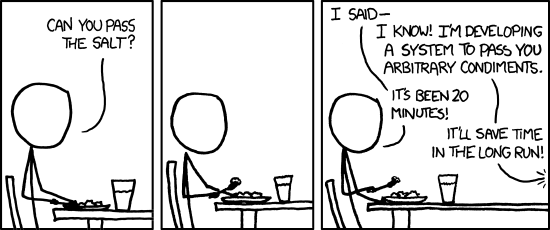
\includegraphics[width=1\linewidth]{programming.png}
	\caption{\label{fig:Programming} But not every task needs to be 
	converted to a computer program --- you will learn to decide when to 
	and when not to write a computer program! \url{http://xkcd.com/974/}} 
\end{wrapfigure}
It is important that you work through the exercises and problems in 
each chapter/section. This document does not tell you every single 
thing you need to know to perform the exercises in it. In programming 
and computing, you learn faster by trying to solve problems (including 
computer crashes!) on your own, often by liberally googling the problem! 

You will be provided guidelines for what makes good or efficient 
solutions to the computing exercises. Later, when you have submitted 
your exercises and practicals, you will be provided solutions. 

Also, every time a mysterious, geeky-sounding term like ``relative 
path'' or ``version control'' appears, please google it!

\section{The goals of this course}

The goal of this course is to teach you to become (or at least show you 
the path towards becoming) a competent quantitative biologist. A large 
part of this involves learning computer programming. Why do biologists 
need to write write computer programs? Here are some (hopefully 
compelling to you!) reasons:

\begin{itemize} \itemsep0pt
	\item Short of fieldwork, programs can do anything (that can be 
	specified). In fact, even fieldwork, if you could one day {\it 
	program} a robot to do it for you \footnote{That way you can potter around
	the forest catching rare butterflies and frogs while the robot does the boring 
	data collecting for you}!  

	\item As such, no software is typically available to perform exactly 
	the analysis you are planning. You should be unhappy if you are 
	trying to shoehorn your data into methods that don't quite seem 
	right.
	
	\item Biological problems and datasets are some of the most 
	complicated imaginable. Programming permits success despite 
	complexity through precise specification	and modularization of 
	complicated analyses. 
	
	\item Modularity -- programming allows you to break up your complex 
	analysis in smaller pieces, yet keep all the pieces in a single, 
	functional analysis.
	 
	\item Reproducibility -- you (or someone else) can just re-run the 
	code to reproduce your analysis. This is also the key to maintaining 
	scientific accountability, integrity, and accuracy.

	\item Organised thinking -- writing code requires you to do this!
	
	\item Career prospects -- good, scientific coders are in short supply 
	in all fields, but most definitely in biology!
	
\end{itemize}

There are several hundred programming languages currently available -- 
which ones should a biologist choose? Ideally, a quantitative biologist 
would like to know:
\begin{enumerate}
	\item A {\it fast}, compiled (or semi-compiled) `procedural' language 
	like {\tt C}
	\item A modern, easy-to-write, interpreted (or semi-compiled) 
	language that is still quite fast, like {\tt python}
	\item A mathematical/statistical software with programming and 
	graphing capabilities like {\tt R}
\end{enumerate}
And all these because one language doesn't fit all purposes. Therefore you 
will learn a few different languages in this course --- hopefully, just 
the right number! Among the languages you will learn here --- {\tt 
python}, 
{\tt R}, and {\tt C} are three of the most popular currently (see
\url{https://www.tiobe.com/tiobe-index/} and \url{ https://goo.gl/vyrqr1}, 
and for some very good reasons.

Our goal is to teach you not just programming, but also good computing 
practices. In this course, you will write plenty of code, deal with 
different data files, and produce text and graphic outputs. You will 
learn to keep your project and coursework organized in logical, 
efficient, error-free and reproducible {\it workflows} (that's a 
mouthful, but an important mouthful).

\section{Some guidelines, conventions and rules} 

\subsection{Beware the dark forces} 

You will NOT be using spreadsheet software (e.g., Excel) in these classes. 
There are times when you will feel the pull of the dark side (ahem!), 
and imagine a more ``comfortable'' world where you are 
mouse-clicking your way happily though Excel-based data manipulations 
and analyses. NO! You will be doing yourself a disservice. On the 
long-ish run you will be much better off visualizing and manipulating 
data on your computer using a programming language like R. This is something you will learn, young {\it padawan}!  

\subsection{Keep your workflow organized}
In the following chapters, you will practice many examples where you 
are required to write large blocks of code. Please get into the habit 
of writing code into text files with an appropriate extension (e.g., 
{\tt *.R} for {\tt R} code, {\tt *.py} for {\tt python} code, etc.). 
Furthermore, please keep all your code files organized in one or more 
directories (e.g., named {\tt Code}!). Similarly, some of these scripts 
will take data files as inputs, and output some results in the form of 
text or graphics. Please keep these inputs and outputs organized as 
well, in separate directories (e.g., named {\tt Data} and {\tt 
Results}) respectively. Your demonstrators and I will help you get set 
up and abide by this ``workflow''. 

\subsection{Conventions used in this document}

Throughout this document, directory paths will be specified in UNIX 
(Mac, Linux) style, using $/$ instead of the \textbackslash{} used in 
Windows. Also, in general, we will be using {\it relative paths} 
throughout the exercises and practicals (more on this later, but google 
it!).

You will find all command line/console arguments, code snippets and 
output in coloured boxes like this:
\begin{lstlisting}
$ ls 
$
\end{lstlisting}
The specific prompt (\$ in this case, belonging to the UNIX terminal) 
will vary with the programming language/console ({\tt \$} for UNIX, 
$>>>$ for Python, {\tt >} for R, etc.).

You will type the commands/code that you see in such boxes 
into the relevant command line (or copy-paste, but not recommended!). I 
have aimed to make the content of this module computer platform (Mac, 
Linux or PC) independent. Also note that:\\

\begin{compactitem}[$\quad\star$]\itemsep4pt
	\item Lines marked with a star like this will be specific 
	instructions for you to follow
\end{compactitem}

\begin{wrapfigure}[20]{c}{0.4\textwidth}
 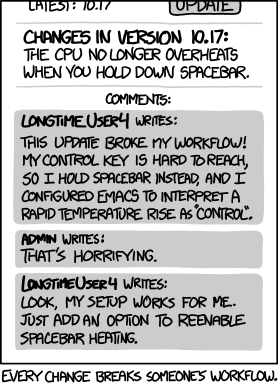
\includegraphics[width=1\linewidth]{workflow.png}
	\caption{\label{fig:Workflows} Logical workflows are important, but 
	don't get married to yours! \url{http://xkcd.com/1172/} } 
\end{wrapfigure}

\subsection{To IDE or not to IDE?}

As you embark on your journey to becoming a competent prectioner of 
biological computing, you will be faced with a hamletian question: ``To 
IDE or not to IDE''. OK, maybe not that dramatic or hamletian... 

An interactive Development Environment (IDE) is a text editor with 
frills that can make life easy by auto-formatting code, running code 
though the terminal or command line, allowing a graphic view of the 
workspace (your active functions, variables, etc.), graphic debugging 
and profiling (you will see these delightful things later), and 
allowing integrated version control (e.g., using {\tt git}). You will 
benefit a lot of you use a code editor that can also offer an IDE 
(e.g., emacs, vim, geany, atom). At the very least, your IDE should offer:
\begin{compactitem}
	\item Auto-indentation
	\item Automatic code wrapping (e.g., keeping lines $<$80 characters 
	long)
	\item Syntax highlighting (e.g., commands vs. variables)
	\item Code folding (fold large blocks of code, say an entire 
	function or loop)
	\item Keyboard control of commenting/uncommenting, code wrapping, etc.
	\item Embedded terminal / shell / commandline console
	\item Sending commands to terminal / shell
\end{compactitem}

And if you end up using multiple programming languages, you will want 
an IDE that can handle them. For example, {\tt RStudio} cannot handle more 
than a fixed set of 2-3 languages. I use {\tt geany}, which has many 
plugins that make multi-language (multilingual?) code development much 
easier. I would also recommend {\tt vim} or {\tt emacs}, which have a 
steeper learning curve, but are very powerful once you have mastered 
them. There are also some new and (increasingly popular) kids on the 
block: {\tt atom} and {\tt vstudio code}.

\subsection{Assessment}

\subsubsection{Undergraduates}

Assessment will be through a computer-based test. You be expected to be 
able to apply the concepts you have learnt to address questions by 
using appropriate R input and interpreting R output. 

\subsubsection{Masters students}

We will assess both your practical computing work itself (including any 
writeups), and whether you are following good programming and workflow 
practices, on a weekly basis. This will be done using scripts --- yes 
we will assess your scripts using scripts! A {\tt python} script will 
check whether your weekly (and version-controlled) directories are neat 
and organized in a logical workflow, and whether all the scripts run 
correctly with the expected inputs and outputs, starting from Week 1 
(Chapter \ref{chap:unix1}). Specifically, as an example towards 
learning good workflow practices, you will keep all your coursework 
code, data inputs and results outputs organized in separate directories 
named {\tt Code}, {\tt Data}, {\tt Results} (or equivalent) 
respectively. 

The assessment script will then record a log file that 
summarizes all the issues found in your workflows, which will be 
emailed to you by the middle of the week (usually on the wednesday) subsequent to the one you 
submitted your weekly practical work in. 

Note that practicals in the weeks/modules not in these notes (e.g., 
GIS, Genomics, Population Genetics) will also be included in the 
assessment. The basic rules you must follow, irrespective of a Week's 
content are: 

\begin{enumerate}
\item All code/scripts go to a {\tt Code} directory

\item All data go to a {\tt Data} directory

\item All results go to a {\tt Results} directory, but the Results 
directory should be empty when you submit your week's work, as it will 
be populated automatically when the assessment script runs.

\item If you have files that don't fit in these categories, put them 
additional, meaningfully named directories (e.g, ``{\tt Writeup}'').

\item No single file should be greater than 100 mb, either data or 
script/code. If a script needs a data file, but the example data file 
is >100 mb, reduce it to a minimum working dataset and upload that,
keeping the main data file(s) under {\tt .gitignore} (more on this 
soon!). Keep the main data backed up of course  \footnote{You could make a 
separate directory called {\tt TestData} as the default input and keep 
the main Data file in the {\tt .gitignore} file --- see Chapter \ref{chap:git}}. 

\item Most importantly, all python, R, bash, and \LaTeX scripts should 
run OK, taking in data and spitting out the results as necessary (these 
are the scripts the assessment code will try to run)

\end{enumerate}

When necessary, more specific, module-specific details on weekly 
coursework and assessment will be given when the module 
starts. 

The computing coursework marking criteria are given in the Appendix 
\ref{chap:Appendices}. 

\subsubsection{The final assessment of weekly coursework}
A written summary assessment of your overall performance with your marks 
will be sent after the end of the 9 weeks. 

The weekly assessments are to help you spot general, as well as 
programming language-specific issues with your computing coursework on 
a regular basis. You may and should fix bugs and other problems that 
feedback logs bring to your attention. I will have a look at how much 
you addressed the issues in the final assessment. The final assessment 
will be necessarily a more subjective than the weekly assessments as we 
are looking to give you an overall picture of how you did and what you 
can improve on. To give you an idea about the criteria for the overall 
assessment, a set of summative marking criteria are also given in Appendix 
\ref{chap:Appendices} titled ``MARKING CRITERIA for EXAMS and ESSAYS 
and COURSEWORK''. 

\begin{center} \it
	Alright, full steam ahead then!
\end{center}

\chapter{Introduction to UNIX and Linux}
\label{chap:unix1}

% check out http://www.ibm.com/developerworks/aix/library/au-badunixhabits.html

\section{What is UNIX?}

UNIX is a machine-independent operating system (OS) developed in the 
1970s by AT\&T programmers (notably Brian Kernighan and Dennis Ritchie, 
fathers of {\tt C}) for programmers (you!). It is multi-user and 
network-oriented by design, uses plain text files for storing data (no 
proprietary file formats), and has a strictly hierarchical directory 
structure (more on this below). This makes it an ideal environment for 
developing your code and storing your data.

Linux and Mac OS are Unix-like (or UN*X or *nix) operating systems that 
have evolved from UNIX. Ubuntu is a Linux distribution.

\section{Why UNIX?}
Here are some good reasons:
 \begin{compactitem}
  \item It was designed for developing code and storing data --- 
  an ideal native habitat for programming languages like Python and R! 
  \item Robust, stable, secure (very few UNIX viruses and malware --- I have never encountered one!) 
  \item Free and open source!
  \item Scores of small programs available to perform simple tasks -- can be 
combined easily
  \item Easy to automate tasks (e.g., using shell scripts)
  \item Multi-user (multiple users can log in concurrently use computer)
  \item Multi-tasking (can perform many tasks at the same time)
  \item Network-ready (easy to communicate between computers)
  \item UNIX has been around since the early 1970's and will likely be 
  around at the end of your career (the hard work you are putting into 
  learning UNIX will pay off over a lifetime!)
  \item Amazing support --- a large body of tutorials and support web 
  sites are readily available online. 
	\item Basically all resources for High-Performance Computing (computer clusters, large workstations, etc.) run a
UNIX or Linux operating system. 
  \end{compactitem}

See \url{http://whylinuxisbetter.net/} (I would have chosen a more 
subtle domain name though!) to aid your brain-washing (cleaning?).

Also, if you like history: {\sloppy \url{https://www.howtogeek.com/182649/htg-explains-what-is-unix}}

\begin{tipbox}
The terms 32-bit and 64-bit refer to the way a computer's processor (also called a CPU), handles information. A 64-bit OS handles large amounts of random access memory (RAM) more effectively than a 32-bit system. Specifically, while 32 bits of information can only access 4 GB of RAM, a 64-bit machine can access essentially unlimited system memory (though this is not yet physically possible)!  
\end{tipbox}  

\section{UNIX directory structure}

\begin{center}
  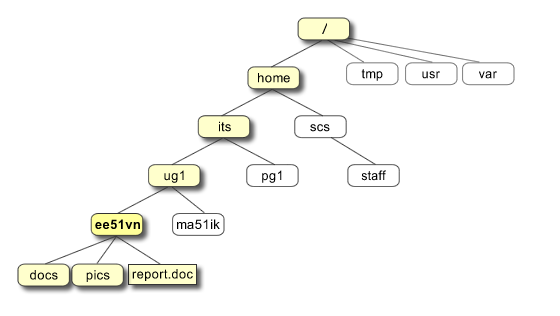
\includegraphics[width=.7\textwidth]{unix-tree.png}\\
  \url{ https://pathanruet.files.wordpress.com/2012/05/unix-tree.png}	
\end{center}

The UNIX directory (same as ``Folder'') structure is hierarchical, with 
a single tree starting from the ``root'' {\tt /}. This is quite unlike 
Windows or MS-DOS, where there are separate trees for disk partitions, 
removable media, network, etc. The key UNIX directories are:
 
\begin{tabular}{p{2cm} p{10cm}} 
 {\tt /} & Is the "root" directory\\
 {\tt /bin} & Contains basic programs\\
 {\tt /etc} & Contains configuration files\\
 {\tt /dev} & Contains files connecting to devices (keyboard,
  mouse, screen, etc.)\\
 {\tt /home} & Your home directory -- this is where you will usually work\\
 {\tt /tmp} & Contains Temporary files\\
\end{tabular}

This hierarchical directory structure makes navigating your 
computer from the terminal/shell (coming up next!) or encoding this 
navigation in your computer programs easier. 

\begin{tipbox}
When you install Linux (say, a Ubuntu version), you will have the opportunity to create separate {\tt swap}, {\tt root} and {\tt home} partitions on your hard disk. {\tt swap} necessarily needs to be a separate partition, while  {\tt root + home} can be on the same partition. If you are a Linux newbie, I suggest that you create a separate {\tt home} partition, even though it is not necessary --- that way, even if you break your linux install, you can easily reinstall it by just wiping the root partition, without losing any of your data (which sits in {\tt home}).  
% In general, you should be fine with a root - only partition between 2GB and 8GB.
\end{tipbox}
  
\section{Meet the UNIX shell}

The shell (or terminal) is a text command processor to interface with 
the Operating System's ``kernel''. We will use the popular (yes, it's 
popular!) {\tt bash} shell. 

\begin{compactitem}[$\quad\star$]\itemsep4pt
	\item To launch {\tt bash} shell, do {\tt Ctrl + Alt + t} (or use {\tt 
Meta} key) --- try it now.
\end{compactitem}

OK, so you have met the shell. Note that:
\begin{compactitem}
   \item The shell automatically starts in your home directory 
  {\tt /home/yourname/}, also called $\sim$ (important to remember!)
   \item Use the {\tt Tab} key -- very handy (try {\tt ls} with {\tt Tab} 
{\tt Tab})
   \item You can navigate commands you previously typed using the up/down arrows  
\end{compactitem}

Other useful keyboard shortcuts are:

\begin{tabular}{p{4.4cm} p{9cm}} 
  {\tt Ctrl + A} & Go to the beginning of the line\\
  {\tt Ctrl + E} & Go to the end of the line\\
  {\tt Ctrl + L} & Clear the screen\\
  {\tt Ctrl + U} & Clear the line before cursor position\\
  {\tt Ctrl + K} & Clear the line after the cursor\\
  {\tt Ctrl + C} & Kill whatever you are running\\
  {\tt Ctrl + D} & Exit the current shell\\
  {\tt Ctrl + right arrow} & Move cursor forward one word\\
  {\tt Ctrl + left arrow} & Move cursor backward one word\\
  \end{tabular}

\section{{\tt sudo}, and installing/removing software}

You can install software in your {\tt /home} directory. In UNIX you 
originally had to login as {\tt root} (administrator). But in Ubuntu, 
it is sufficient to add {\tt sudo} ({\tt s}uper {\tt u}ser {\tt do}) in 
front of a command: 
\begin{lstlisting}
sudo apt-get install geany geany-plugins geany-plugin-latex 
geany-plugin-addons
\end{lstlisting}

You can install anything that is in the Ubuntu "repository". Let's try 
installing something else --- a weather indicator that I think really works
very well. 

But here you have to first install the repository: 
\begin{lstlisting}
$ sudo add-apt-repository ppa:atareao/atareao
\end{lstlisting}

This will ask you to first approve the additon of this repository. Then 
update the repository packages, 
\begin{lstlisting}
$ sudo apt-get update 
\end{lstlisting}

And then install,
\begin{lstlisting}
$ sudo apt-get install my-weather-indicator
\end{lstlisting}

\begin{center}
	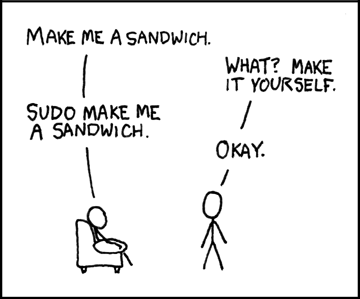
\includegraphics[width = 0.4\linewidth]{sandwich.png}\\
	{\tt http://xkcd.com/149/}
\end{center}					

You can also easily remove software by, well, using the {\tt remove} 
command! You will find that commands names are quite intuitive, as they 
should be. If you think a command with a certain name should exist, it 
very often does!

\begin{lstlisting}
$ sudo apt-get remove indicator-messages
\end{lstlisting}

This will get rid of the evolution mail indicator --- very unlikely 
that you will use evolution!

\section{Basic UNIX commands}
 
\begin{tabular}{p{.3\textwidth} p{.7\textwidth}} 
 {\tt man [COMMAND]} & Show help page of a command.\\
 {\tt whoami} & Display your user-name.\\
 {\tt pwd} & Show the current directory.\\
 {\tt ls} & List the files in the directory.\\
 {\tt cd [DIRNAME]} & Change directory.\\ 
 {\tt cd ..} & Move one directory up. \\
 {\tt cd /} & Go to the root directory. \\
 {\tt cd $\sim$} or just {\tt cd } & Go to the home directory.\\
 {\tt cp [FROM] [TO]} & Copy a file or directory non-recursively (what's this?).\\
 {\tt mv [FROM] [TO]} & Move or rename a file or directory.\\
 {\tt touch [FILENAME]} & Create an empty file.\\
 {\tt echo "My string"} & Print a string (here, "My string").\\
 {\tt rm [TOREMOVE]} & Remove a file or directory non-recursively.\\
 {\tt mkdir [DIRNAME]} & Create a directory.\\
 {\tt rmdir [DIRNAME]} & Remove an empty directory.\\
 {\tt wc [FILENAME]} & Count the number of lines and words in a file.\\
 {\tt sort [FILENAME]} & Sort the lines of a file and print result.\\
 {\tt uniq } & Shows only unique elements of a list.\\
 {\tt cat [FILENAME]} & Print the file on the screen.\\
 {\tt less [FILENAME]} & Progressively print a file on the screen ("q" 
 to exit).\\
 {\tt head [FILENAME]} & Print the first few lines of a file.\\
 {\tt tail [FILENAME]} & Print the last few lines of a file.\\
 {\tt history} & Show the last commands you typed.\\
 {\tt date} & Print current date.\\
 {\tt file [FILENAME]} & Determine the type of a file.\\
 {\tt passwd} & Change user password.\\
 {\tt chmod [FILENAME]} & Change file permissions.
\end{tabular}
  
\section{Building your coursework directory structure}

It is time to start building your CMEE coursework directory structure. 
Please follow these rules:
	\begin{compactitem}

		\item Do all your work in {\tt CMEECourseWork}, located in a 
		suitable place in your {\tt /home} (make mama proud, keep your {\tt 
		home} organized!)
	 \item Each week's coursework should be in its respective directory: 
	 {\tt CMEECourseWork/Week1}, {\tt CMEECourseWork/Week2}, etc
	 \item Each week's directory will contain directories called {\tt 
	 Code}, {\tt Data}, etc (later)
		\item You will bring {\tt CMEECourseWork} and all it's contents 
			 under version control using Git (later)
  \end{compactitem}

\begin{tipbox}
Don't forget to use the {\tt tab} key. It autocompletes directory 
names for you (same in {\tt R} and {\tt Python}, and/or provides  
a list of files in the current directory (hit {\tt tab} twice after 
certain commands. For example, try double tab after typing {\tt ls} 
at the bash prompt.)  	
\end{tipbox}

\begin{compactitem}[$\quad\star$]\itemsep4pt
	\item OK, {\tt mkdir} your {\tt CMEECourseWork} directory now.
\end{compactitem}
Starting by creating {\tt CMEECourseWork}). Then,

\begin{lstlisting}
$ mkdir Week1
$ cd Week1
$ mkdir sandbox
$ cd Sandbox
bash: cd: Sandbox: No such file or directory
$ cd ..
$ rm sandbox
rm: cannot remove `sandbox/`: Is a directory
$ mv sandbox Sandbox # OR, "rm -r sandbox" (careful with the -r option!)
\end{lstlisting}

Note the hash mark \# above --- anything after a \# is ignored (so you 
can use it for commenting).

\begin{lstlisting}
$ cd Sandbox
$ pwd
$ ls
$ touch TestFile # OR, "touch TestFile.txt"
$ ls
$ mv TestFile TestFile2
$ rm TestFile2
\end{lstlisting}

You could have made your project directories and subdirectories in one 
swoop by using the {\tt -p} option of {\tt mkdir}: 

\begin{lstlisting}
$ mkdir -p CMEECourseWork/Week1/{Data,Code,Sandbox}
\end{lstlisting}

% Note: ``$\textbackslash$'' means multi-line code (can be entered verbatim
% in bash/terminal)
 
\section{Command arguments}

Most UNIX commands accept arguments that modify their behavior. E.g.,  {\tt ls 
-l} (ls ``minus''l) lists the files in longer format. Some useful 
arguments:
 
\begin{tabular}{p{.4\textwidth} p{.6\textwidth}} 

{\tt cp -r [DIR1] [DIR2]} & Copy a directory recursively (i.e., including 
all the sub-directories and files).\\
{\tt rm -i [FILENAME]} & Remove a file, but asks first (for safety).\\
{\tt rm -r [DIR]} & Remove a directory recursively (i.e., including all the 
sub-directories and files).\\
{\tt ls -a} & List all files, including hidden ones.\\
{\tt ls -h} & List all files, with human-readable sizes (Mb, Gb).\\
{\tt ls -l} & List all files, long format.\\
{\tt ls -S} & List all files, order by size.\\
{\tt ls -t} & List all files, order by modification time.\\
{\tt ls -1} & List all files, one file per line.\\
{\tt mkdir -p Dir1/Dir2/Dir3} & Create the directory Dir3 and Dir1 and 
Dir2 if they do not already exist.\\
{\tt sort -n} & Sort all the lines, but use numeric values
  instead of dictionary (i.e., 11 follows 2).\\
\end{tabular}

You can also combine command arguments. Try:
\begin{lstlisting}
$ ls -1t #combines -l and -t
\end{lstlisting}

\section{Redirection and pipes}

Output of programs can also be ``redirected'' to a file:

\begin{tabular}{p{.1\textwidth} p{.9\textwidth}} 
  {\tt >} & Redirect output from a command to a file on disk. If
    the file already exists, it will be overwritten.\\
  {$>>$} & Append the output from a command to a file on disk. If
    the file does not exist, it will be created.\\
\end{tabular}
 
Examples (make sure you are in {\tt Week1/Sandbox}):
      
\begin{lstlisting}
$ echo "My first line." > test.txt
$ cat test.txt
$ echo "My second line" >> test.txt
$ ls / >> ListRootDir.txt
$ cat ListRootDir.txt #Isn't that cool?!
\end{lstlisting}
 
We can also concatenate commands using ``pipes'' with ``$\vert$'' e.g., 
to count how many files are in root (/) directory:
\begin{lstlisting}
$ ls / | wc -l # what does this do? Look up "man wc"
\end{lstlisting}
Or try
\begin{lstlisting}
$ ls -lt | head -5 #what does this do?
\end{lstlisting}

\section{Wildcards}

We can use wildcards to find files based on their names (again, in 
{\tt Week1/Sandbox} !):
 
\begin{lstlisting}
$ mkdir TestWild
$ cd TestWild
$ touch File1txt
$ touch File2.txt
$ touch File3.txt
$ touch File4.txt
$ touch File1.csv
$ touch File2.csv
$ touch File3.csv
$ touch File4.csv
$ touch Anotherfile.csv
$ touch Anotherfile.txt
$ ls 
$ ls | wc -l
\end{lstlisting}

We will use the following wildcards:

\begin{tabular}{p{.2\textwidth} p{.8\textwidth}} 
  {\tt ?} & Any single character, except a leading dot (hidden 
  files).\\
  {\tt *} & Zero or more characters, except a leading dot (hidden 
  files).\\
	{\tt [A-Z]} & Define a class of characters (e.g., upper-case 
	letters).\\
\end{tabular}
 
Now let's try to find the files using wildcards:

\begin{lstlisting}
$ ls *
$ ls File*
$ ls *.txt
$ ls File?.txt
$ ls File[1-2].txt
$ ls File[!3].*
\end{lstlisting}

\section{Using {\tt grep}}

{\tt grep} is a command that matches strings in a file (why is this 
useful?). It is based on regular expressions (more on this later). 
Let's explore some basic usage of {\tt grep}. For a test file let's 
download a list of protected species from the UN website (to 
{\tt Sandbox}):
 
\begin{lstlisting}
$ wget http://www.cep.unep.org/pubs/legislation/spawannxs.txt #Cool!
$ head -n 50 spawannxs.txt #You will see "head" in R as well
\end{lstlisting}

Now,

\begin{lstlisting}
$ mkdir ../Data #Note the relative path "../"
$ mv spawannxs.txt ../Data/
$ cd ../Data
$ head -n 50 spawannxs.txt 
\end{lstlisting}

Note that now you have a {\tt Data} directory. 

OK, what about falcons? 
 
\begin{lstlisting}
$ grep Falco spawannxs.txt
Falconidae	Falco		femoralis septentrionalis
Falconidae	Falco		peregrinus
Falconidae	Polyborus	plancus
Falconidae	Falco		columbarius
\end{lstlisting}

Using {\tt -i} make the matching case-insensitive:
 
\begin{lstlisting}
$ grep -i Falco spawannxs.txt
Order:	FALCONIFORMES
Falconidae	Falco		femoralis septentrionalis
Falconidae	Falco		peregrinus
Falconidae	Polyborus	plancus
Order:	FALCONIFORMES
Order:	FALCONIFORMES
Order:	FALCONIFORMES
Falconidae	Falco		columbarius
\end{lstlisting}

Now let's find the beautiful ``Ara'' macaws:
\begin{center}
  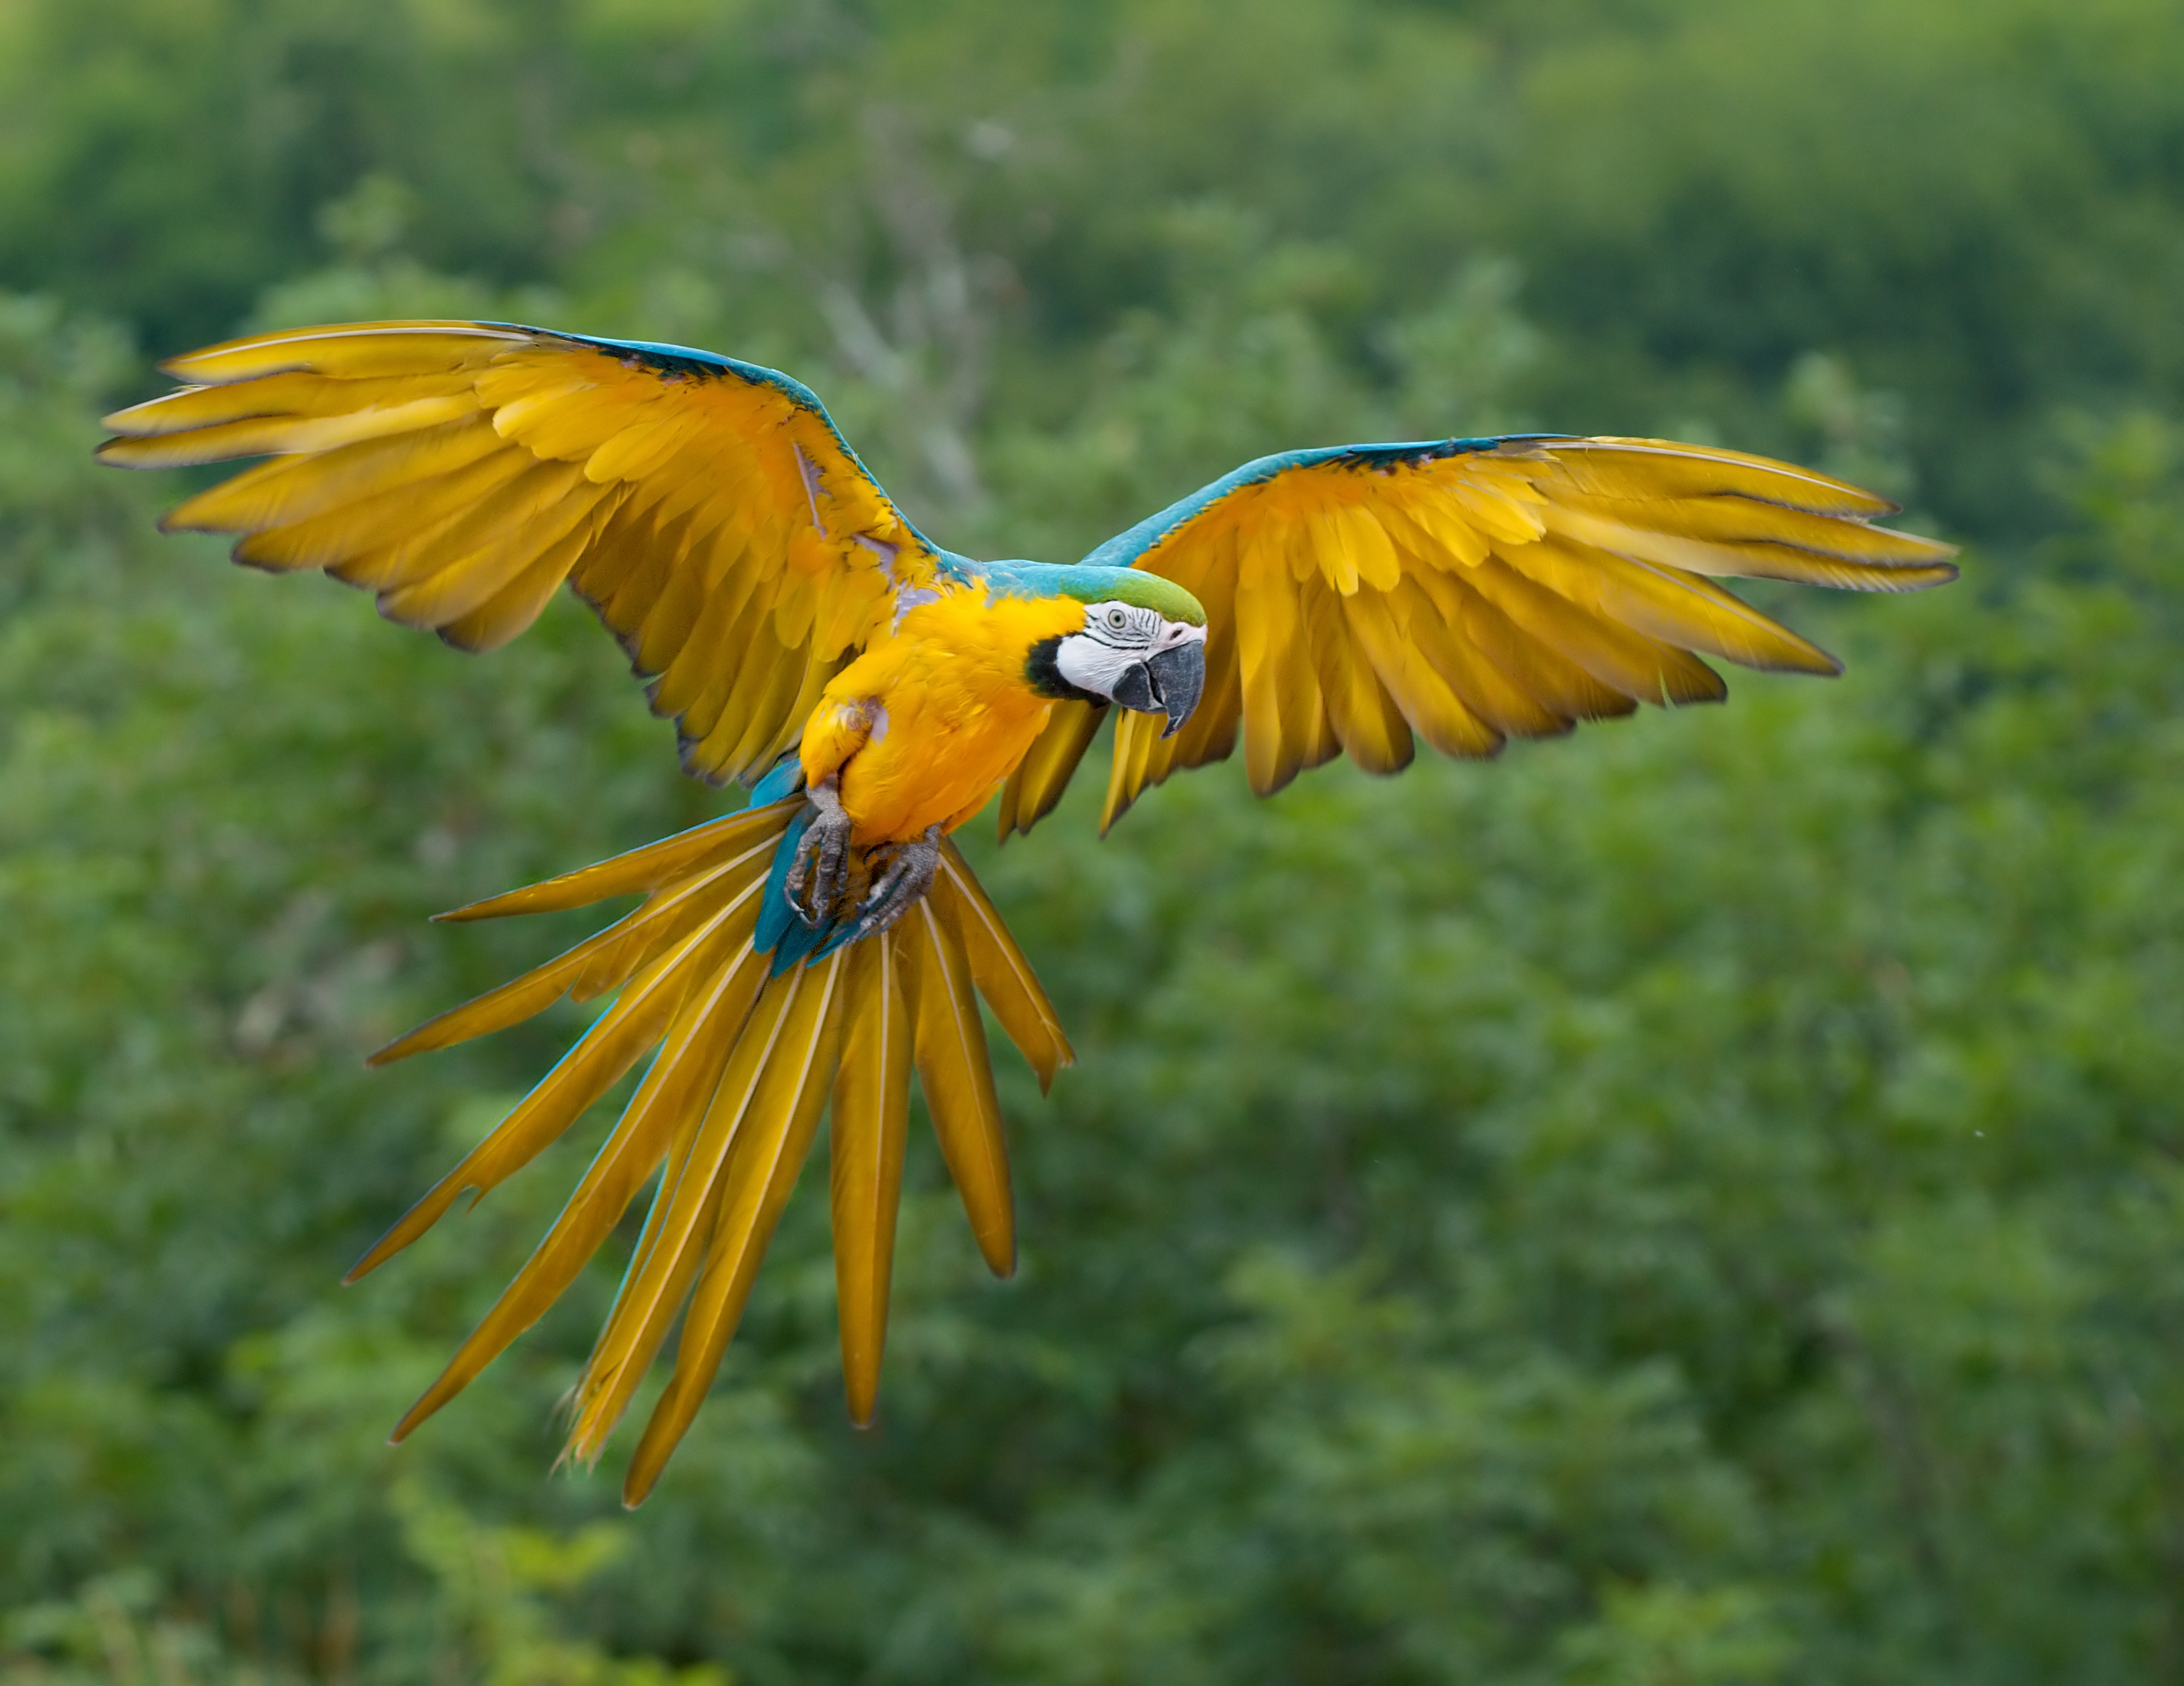
\includegraphics[width=.7\textwidth]{Ara_ararauna.jpg}
\end{center}

But this poses a problem (what is the problem?):

\begin{lstlisting}
$ grep -i ara spawannxs.txt
Flacourtiaceae	Banaras		vanderbiltii
Order:	CHARADRIIFORMES
Charadriidae	Charadrius	melodus
Psittacidae	Amazona		arausica
Psittacidae	Ara		macao
Dasyproctidae	Dasyprocta	guamara
Palmae		Syagrus (= Rhyticocos)	amara
Psittacidae	Ara		ararauna
Psittacidae	Ara		chloroptera
Psittacidae	Arao		manilata
Mustelidae	Eira		barbara
Order:	CHARADRIIFORMES
\end{lstlisting}

We can solve this by specifying {\tt -w} to match only full words:
 
\begin{lstlisting}
$ grep -i -w ara spawannxs.txt
Psittacidae	Ara		macao
Psittacidae	Ara		ararauna
Psittacidae	Ara		chloroptera
\end{lstlisting}

And also show line(s) after the one that was  matched, we can use {\tt 
-A x}, where {\tt x} is number of lines to use:

\begin{lstlisting}
$ grep -i -w -A 1 ara spawannxs.txt
Psittacidae	Ara		macao

--
Psittacidae	Ara		ararauna
Psittacidae	Ara		chloroptera
Psittacidae	Arao		manilata
\end{lstlisting}

Similarly, {\tt -B} shows the lines before:
 
\begin{lstlisting}
$ grep -i -w -B 1 ara spawannxs.txt
Psittacidae	Amazona		vittata
Psittacidae	Ara		macao
--
Psittacidae	Amazona		ochrocephala
Psittacidae	Ara		ararauna
Psittacidae	Ara		chloroptera
\end{lstlisting}

Use {\tt -n} to show the line number of the match:
 
\begin{lstlisting}
$ grep -i -w -n ara spawannxs.txt
216:Psittacidae	Ara		macao
461:Psittacidae	Ara		ararauna
462:Psittacidae	Ara		chloroptera
\end{lstlisting}

To print all the lines that do not match a pattern, use {\tt -v}:
 
\begin{lstlisting}
$ grep -i -w -v ara spawannxs.txt
\end{lstlisting}

To match one of several strings, use {\tt grep 
"string1$\backslash\vert$string2" file}. {\tt grep} can be used on 
multiple files, all files, using wildcards for filenames, etc -- 
explore as and when you need.

\section{Finding files with {\tt find}}

Its's easy to find files in UNIX using {\tt find}! Let's test it (make 
sure you are in {\tt Sandbox}, not {\tt Data}!)
 
\begin{lstlisting}
$ mkdir TestFind
$ cd TestFind
$ mkdir -p Dir1/Dir11/Dir111 #what does -p do?
$ mkdir Dir2
$ mkdir Dir3
$ touch Dir1/File1.txt
$ touch Dir1/File1.csv
$ touch Dir1/File1.tex
$ touch Dir2/File2.txt
$ touch Dir2/file2.csv
$ touch Dir2/File2.tex
$ touch Dir1/Dir11/Dir111/File111.txt
$ touch Dir3/File3.txt
\end{lstlisting}

Now find particular files:
 
\begin{lstlisting}
$ find . -name "File1.txt"
./Dir1/File1.txt
\end{lstlisting}

Using {\tt -iname} ignores case, and you can use wildcards:
 
\begin{lstlisting}
$ find . -iname "fi*.txt"
./Dir1/File1.txt
./Dir1/Dir11/Dir111/File111.txt
./Dir3/File3.txt
./Dir2/File2.txt
\end{lstlisting}

You can limit the search to exclude sub-directories:
 
\begin{lstlisting}
$ find . -maxdepth 2 -name "*.txt"
./Dir1/File1.txt
./Dir3/File3.txt
./Dir2/File2.txt
\end{lstlisting}

You can exclude certain files:
 
\begin{lstlisting}
$ find . -maxdepth 2 -not -name "*.txt"
.
./Dir1
./Dir1/File1.tex
./Dir1/File1.csv
./Dir1/Dir11
./Dir3
./Dir2
./Dir2/File2.tex
./Dir2/File2.csv
\end{lstlisting}

To find only directories:
 
\begin{lstlisting}
$ find . -type d
.
./Dir1
./Dir1/Dir11
./Dir1/Dir11/Dir111
./Dir3
./Dir2
\end{lstlisting}

\begin{tipbox}
There are are many ways in which you can tweak your Linux/UNIX 
environment and bash/terminal to your likes. For example, see 
\url{http://www.howtogeek.com/tag/ubuntu/ubuntu-tips/}.

But be careful, it can be addictive, and sometimes dangerous to your 
system's stability! 

Here are a couple of tweaks that I really find useful:\\

{\it Opening nautilus from terminal}

In terminal you can enter "f" to open nautilus in current directory 
by doing the following. Open your {\tt .bashrc} for editing:

\begin{lstlisting}
$ sudo gedit ~/.bashrc
\end{lstlisting}

Then add to the last line (type it, don't copy and paste!):\\
{\tt alias f='nautilus .'}

Then restart terminal or in current terminal:
\begin{lstlisting}
$ source ~/.bashrc
\end{lstlisting}

{\it Enabling autocomplete in terminal}

What happens when you use up and down keys in terminal? If nothing, 
then you need to enable reverse searching history. To do so, open 
{\tt /etc/inputrc}

\begin{lstlisting}
$ sudo geany /etc/inputrc
\end{lstlisting}

Then, add the following to it:

\begin{lstlisting}
## arrow up
"\e[A":history-search-backward
## arrow down
"\e[B":history-search-forward
\end{lstlisting}


Then close current terminal, open new one, and try up and down keys 
again.
\end{tipbox}
	      
\section[]{Practical: Make sure the basics work}
 
 \begin{enumerate} \itemsep10pt
		
		\item {\bf Some instructions}: 
		
		Review (especially if you got lost along the way) and make 
		sure you can run and understand all the commands and get the 
		expected outputs we have covered today. 
		
		Make sure you have your directory organized with {\tt Data} 
		and {\tt Sandbox} with the necessary files, under {\tt 
		CMEECourseWork/Week1}.

		Along with the completeness of the practicals/exercises 
		themselves, you will be marked on the basis of how complete and 
		well-organized your directory structure and content is -- in all 
		coming weeks as well.

	\item Here is a more complicated bash command using two pipes {\it you 
	are not expected to include the answer to this one as part of your 
	weekly submission}:
	
\begin{lstlisting}
$ find . -type f -exec ls -s {} \; | sort -n | head -10
\end{lstlisting}

% Sort and head to find the largest 10 files, including in 
% sub-directories. A faster option would be 
% find . -type f -exec ls -s {} + | sort -n | head -10
% See {\tt man find}, especially the part about the {\tt -exec option}

% Basically, -exec runs a command ({\tt ls -s} in this case) on each of 
% the files found, {} is replaced with the name of each file found, 
% and the find command is terminated by \;

	What does this command do (Hint: try it on the test directories and 
	files we created in {\tt Sandbox})?
		
	Note that along with the {\tt man} command, you can use the internet 
	 to get help on practically everything about UNIX!

\item In the directory {\tt /Data/fasta} you find some FASTA files. 
These files have an header starting with $>$ followed by the name of 
the sequence and other metadata. Starting from the second line, we have 
the sequence data. Write a file called {\tt UnixPrac1.txt} with UNIX 
shell commands that do the following (number each command with a hashed 
comment like so -- \# 1, \# 2, etc):

    \begin{enumerate}
    
     \item Count how many lines are in each file
     % %%wc -l *.fasta

     \item Print everything starting from the second line for the {\tt E. 
coli} genome
     % %%tail -n+2 407228326.fasta

    \item Count the sequence length of this genome
     % %%tail -n+2 407228326.fasta | tr -d "\n"
     % %%tail -n+2 407228326.fasta | tr -d "\n" | wc -c

     \item Count the matches of a particular sequence, ``ATGC'' in
the genome of \textit{E. coli} (hint: Start by removing the first line 
and removing newline characters)
     
  % %%   tail -n+2 407228326.fasta | tr -d "\n" | grep -o "ATGTACATA"

   % %%  tail -n+2 E.coli.fasta | tr -d "\n" | grep -o "ATGC" | wc -l

    \item Compute the AT/GC ratio
    
  % %%  tail -n+2 E.coli.fasta | tr -d "\n" | grep -o [A,T] | wc -l
  % %%  tail -n+2 E.coli.fasta | tr -d "\n" | grep -o [G,C] | wc -l
   
    \end{enumerate}
    
Save {\tt UnixPrac1.txt} in the {\tt Code} directory. Please make sure 
that each command calls the data from the {\tt Data} directory! Do not 
write any of the above as shell scripts (that's not been covered yet; 
see Chapter \ref{chap:sscripting})  --- each one should be a single 
line solution made of (potentially piped together) UNIX commands.

{\bf Please put (judicious) comments in any of your script files. But 
you won't be penalized if you haven't put in comments in the first week 
in practicals. From the first Python week (Chapter \ref{chap:pythonI}) 
onwards, you will be penalizeed if you don't properly document and 
comment code (more on this next week), even if you weren't explicitly 
asked to.}

\end{enumerate}

\section{Readings \& Resources}
IC library gives you with access to several e- and paper books on UNIX, some 
specific to Ubuntu. Browse or search and find a good intro book.

\begin{itemize} \itemsep6pt
    \item Lots of UNIX tutorials out there. Try 
\url{http://software-carpentry.org/lessons.html} (Chapter ``shell'').
	\item Some good UNIX usage habits: \url{http://www.ibm.com/developerworks/aix/library/au-badunixhabits.html}
   \item List of UNIX commands along with man page: \url{http://archive.oreilly.com/linux/cmd/}
\end{itemize}

\chapter{Advanced UNIX: Shell scripting}
\label{chap:sscripting}
 
\section{Shell scripting: What and Why}
 
Instead of typing all the UNIX commands we need to perform one after 
the other, we can save them all in a file (a ``script'') and execute 
them all at once.

The {\tt bash} shell we are using provides a proper syntax that can be 
used to build complex command sequences and scripts. 

Scripts can be used to automate repetitive tasks, to do simple data 
manipulation or to perform maintenance of your computer (e.g., backup). 
Indeed, most data manipulation can be handled by scripts without the 
need of writing a proper program. 

\section{Scripting: How}

There are two ways of running a script, say {\tt myscript.sh}:
 
\begin{enumerate}\itemsep6pt
	\item The first is to call the interpreter bash to run the file (try 
	this, but won't work as you don't have a {\tt myscript.sh} script !)
\begin{lstlisting}
$ bash myscript.sh # OR sh myscript.sh
\end{lstlisting}
(A script that does something specific in a given project)

\item OR, make the script executable and execute it:
\begin{lstlisting}
$ chmod +x myscript.sh
$ myscript.sh
\end{lstlisting}
(A script that does something generic, and is likely to be reused again 
and again -- can you think of examples?)

\end{enumerate}
The generic scripts of type (2) can be saved in {\tt username/bin/}
and made executable (the {\tt .sh} extension not needed)
\begin{lstlisting}
$ mkdir ~/bin
$ PATH=$PATH:$HOME/bin #Tell UNIX to look in /home/bin for commands
\end{lstlisting}



\section{Your first shell script}

Let's write our first shell script! For starters,
 \begin{compactitem}[$\quad\star$]\itemsep4pt{}
	\item Write and save {\tt boilerplate.sh} in {\tt 
	CMEECourseWork/Week1/Code}, and add the following script to it (type 
	it in a code editor like geany):
	\end{compactitem}
		
	\lstinputlisting[language=bash]{Practicals/Code/boilerplate.sh}
The first line is a ``shebang'' (or sha-bang or hashbang or pound-bang 
or hash-exclam or hash-pling! -- Wikipedia). It can also can be written 
as {\tt \#!/bin/sh}. It tells the bash iterpreter that this is a bash 
script and that it should be interpreted and run as such. The hash 
marks in the following lines tell the interpreter that it should ignore 
the lines following them (that's how you put in script documentation 
(who wrote the script and when, what the script does, etc.) and 
comments on particular line of script.
\begin{tipbox}
	Geany users can enable send lines of code directly to terminal using a 
	keyboard key combination through two configuration steps: 
	\begin{enumerate}
		\item Enable ``Send Selection to Terminal''	with the {\tt 
		<Primary>Return} keys by going to geany's {\tt Edit > Preferences > 
		Keybindings} menu item. 
		\item Now edit (e.g., using geany) the file {\tt geany.conf}. You 
		can use geany itself to this:
\begin{lstlisting}
$ geany ~/.config/geany/geany.conf
\end{lstlisting}
		This will open {\tt geany.conf} in geany. In this file, set {\tt 
		send\_selection\_unsafe=true}, then close the file, and restart 
		geany. 
	\end{enumerate} 
\end{tipbox}

Now run your boilerplate shell script by typing in the terminal:
\begin{lstlisting}
$ bash boilerplate.sh
\end{lstlisting}

\section{A useful shell-scripting example}
Let's write a shell script to transform comma-separated files (csv) to 
tab-separated files and vice-versa. This can be handy --- for example, 
in certain computer languages, it is much easier to read tab or space 
separated files than csv (e.g., {\tt C})

To do this, in the bash we can use {\tt tr}, which deletes or 
substitute characters. Here are some examples.
\begin{lstlisting}
$ echo "Remove    excess      spaces." | tr -s "\b" " "
Remove excess spaces.
$ echo "remove all the as" | tr -d "a"
remove ll the s
$ echo "set to uppercase" | tr [:lower:] [:upper:]
SET TO UPPERCASE
$ echo "10.00 only numbers 1.33" | tr -d [:alpha:] | tr -s " " ","
10.00,1.33

\end{lstlisting}
 
Now write a shell script to substitute all tabs with commas called
{\tt tabtocsv.sh} in {\tt Week1/Code}:

\lstinputlisting[language=bash]{Practicals/Code/tabtocsv.sh}
 
Now test it (note where the output file gets saved)
\begin{lstlisting}
echo -e "test \t\t test" >> ../SandBox/test.txt
bash tabtocsv.sh ../SandBox/test.txt
\end{lstlisting}

\section{Variables in shell scripting}

There are three ways to assign values to variables (note lack of
spaces!):
  \begin{enumerate}
    \item Explicit declaration: {\tt MYVAR=myvalue}
    \item Reading from the user: {\tt read MYVAR}
    \item Command substitution: {\tt MYVAR=\$( (ls | wc -l) )}
\end{enumerate}

Here are some examples of assignments (try it out save as {\tt 
Week1/Code/variables.sh}):

{\tiny \lstinputlisting[language=bash]{Practicals/Code/variables.sh}}

And also (save as {\tt Week1/Code/MyExampleScript.sh}): 

\lstinputlisting[language=bash]{Practicals/Code/MyExampleScript.sh}

\section{Some more Examples}

Here are a few more illustrative examples (test each one out, save in
{\tt Week1/Code/} with the given name):

{\tt CountLines.sh}:
\lstinputlisting[language=bash]{Practicals/Code/CountLines.sh}

{\tt ConcatenateTwoFiles.sh}:
\lstinputlisting[language=bash]{Practicals/Code/ConcatenateTwoFiles.sh}

\section[Practical]{Practical}
  \begin{enumerate} \itemsep10pt
		\item {\bf Some instructions}:
		
		Along with the completeness of the practicals/exercises themselves, 
		you will be marked on the basis of how complete and well-organized 
		your directory structure and content is. 

		Review (especially if you got lost along the way) and make sure all 
		your shell scripts are functional: {\tt boilerplate.sh}, {\tt 
		ConcatenateTwoFiles.sh}, {\tt CountLines.sh},\\ {\tt 
		MyExampleScript.sh}, {\tt tabtocsv.sh}, {\tt variables.sh}
		
		Don't worry about how some of these scripts will run on my computer 
		without explicit inputs (e.g., {\tt ConcatenateTwoFiles.sh} needs 
		two input files) --- I will run them with my own test files.

	 Make sure you have your weekly directory organized with {\tt Data}, {\tt 
	 Sandbox}, {\tt Code} with the necessary files, under {\tt 
	 CMEECourseWork/Week1}. {\it All scripts should run on any other 
	 Unix/Linux machine} --- for example, always call data from the {\tt 
	 Data} directory using relative paths.
	 
		{\bf Make sure there is a {\tt readme} file in every week's 
		directory. This file should give an overview of the weekly 
		directory contents, listing all the scripts and what they do. This 
		is different from the {\tt readme} for your overall git repository, 
		of which {\tt Week 1} is a part. You will write a similar {\tt 
		readme} for each subsequent weekly submission.  

		Don't put any scripts that are part of the submission in 
	 your {\tt \/home/bin} directory! You can put a copy there, but a 
	 working version should be in your repository.}
   
   
	 \item Finally, a small exercise: write a {\tt csvtospace.sh} shell 
	 script that takes a {\tt c}omma {\tt s}eparated {\tt v}alues and 
	 converts it to a space separated values file. However, it must not 
	 change the input file --- it should save it as a differently named 
	 file. 
	 
	 Save the script in {\tt CMEECourseWork/Week1/Code}, and run it on the 
	 {\tt csv} data files that are in {\tt Temperatures} in the master 
	 repository's {\tt Data} directory. 
	 
	 {\it Don't modify anything (or refer to anything) in your local copy 
	 of the master repository. All changes you make in the master 
	 repository will be lost. Copy whatever you need from the master 
	 repository to your own repository.}
    
   \end{enumerate}

\begin{center}
	\it Commit and push everything by next Wednesday 5 PM.
\end{center} 

This includes {\tt UnixPrac1.txt}! Check the updated instructions from 
Chapter \ref{chap:unix1} on this practical.

% Look at makefile in Unix for gluing workflows	

\section{Readings \& Resources}

  \begin{itemize} 
		\item Plenty of shell scripting resources and tutorials out there; 
		in particular, look up 
		\url{http://www.tutorialspoint.com/unix/unix-using-variables.htm}
  
  \end{itemize}

\chapter{Version control with Git}
\label{chap:git}

\section{What is Version Control?}

Version control, also known as revision control or source control, is 
the management and tracking of changes to documents, computer programs, 
large web sites, and other collections of information in an automated 
way.

Any project (collections of files in directories) under version control 
has changes and additions/deletions to its files and directories 
recorded and archived over time so that you can recall specific 
versions later. With version control of biological computing projects, 
you can:

 \begin{compactitem}\itemsep10pt{}
 
		\item record of all changes made to a set of files and directories, 
		including text (usually ASCII) data files, so that you can access 
		any previous version of the files

    \item branch (and merge) new projects

		\item ``roll back'' data, code, documents that are in plain text 
		format (other file formats can also be versioned; see section on 
		binary files below). 
	
	\end{compactitem}
 
Note also that version control (usually git) is in fact the technology 
embedded in the versioning of various word processor and  
spreadsheet applications (e.g., Google Docs, Sheets, Overleaf). 

\begin{figure} \centering
  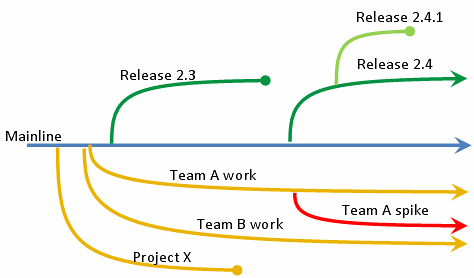
\includegraphics[width=.5\textwidth]{VC.png}
  \caption{A general idea of how version control works.}
\end{figure}

\section{Why Version Control?}

{\centering  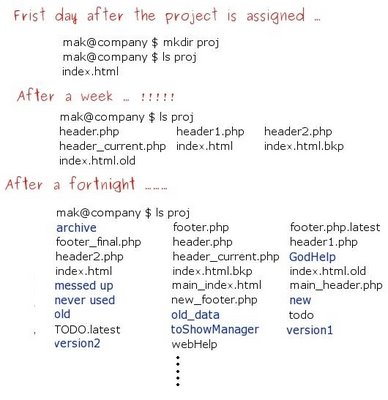
\includegraphics[width=.5\textwidth]{cvs.png}\\
  \tt 
maktoons.blogspot.com/2009/06/if-dont-use-version-control-system.html}
 
 Or here's another one: \url{http://www.phdcomics.com/comics/archive/phd101212s.gif} 
  
\section{git}

We will use git, developed by Linus Torvalds, the ``Linu'' in Linux. In 
git each user stores a complete local copy of the project, including the 
history and all versions. So you do not rely as much on a centralized 
(remote) server. We will use bitbucket.org -- it gives you unlimited 
free private repositories if you register with an academic email! 
First, install and configure {\tt git}:

\begin{lstlisting} 
$ sudo apt-get install git
$ git config --global user.name "Your Name"
$ git config --global user.email "your.login@imperial.ac.uk"
$ git config --list
\end{lstlisting}

\section{Your first repository}

Time to bring your {\tt CMEECourseWork} under version control:

\begin{lstlisting} 
$ cd CMEECourseWork
$ git init
$ echo "My CMEE 2016-17 Coursework Repository" > README.txt
$ git config --list
$ ls -al
$ git add README.txt #Staging
$ git status
$ git commit -m "Added README file." #you can use -am too
$ git status #what does it say now?
$ git add -A
$ git status
\end{lstlisting} 

Nothing has been sent to a remote server yet (see section 
\ref{ssec:git_comds})! So let's go to your git service (bitbucket or 
github) and setup:

 \begin{compactitem}[$\quad\star$]\itemsep4pt
	\item Login to your bitbucket or github account
	\item \sloppy Set up your {\tt ssh} based access 
	
	bitbucket:
	\url{https://confluence.atlassian.com/bitbucket/set-up-ssh-for-git-728138079.html} 
	
	github: \url{https://help.github.com/articles/connecting-to-github-with-ssh}
  
  \item Then create repository there with name {\tt CMEECourseWork}
	
	\item \sloppy Then grab the repository url and use {\tt git remote add origin 
	https...} 
	
	bitbucket:  \url 
	{https://confluence.atlassian.com/bitbucket/set-up-a-repository-877174034.html}
	
	github: \url{https://help.github.com/articles/adding-an-existing-project-to-github-using-the-command-line/}
	
 \end{compactitem}
  	  
You are done. Now let's learn to use git! 

\section{{\tt git} commands}
  
Here are some basic git commands:
 
\begin{tabular}{p{.3\textwidth} p{.7\textwidth}} 
	{\tt git init} & Initialize a new repository\\
	{\tt git clone} & Download a repository from a remote server\\
	{\tt git status} & Show the current status\\
	{\tt git diff} & Show differences between commits\\
	{\tt git blame} & Blame somebody for the changes!\\
	{\tt git log} & Show commit history\\
	{\tt git commit} & Commit changes to current branch\\
	{\tt git branch} & Show branches\\
	{\tt git branch name} & Create new branch\\
	{\tt git checkout name} & Switch to a different commit/branch\\
	{\tt git pull} & Upload from remote repository\\
	{\tt git push} & Send changes to remote repository\\
\end{tabular}

\subsection{{\tt git} command structure}
\label{ssec:git_comds}
Here is a graphical outline of the git command structure. Note that 
only when you {\tt push} or  {\tt fetch} do you need an internet 
connection, as before that you are only archiving in a local (hidden) 
repository. 
 
  \begin{center}
		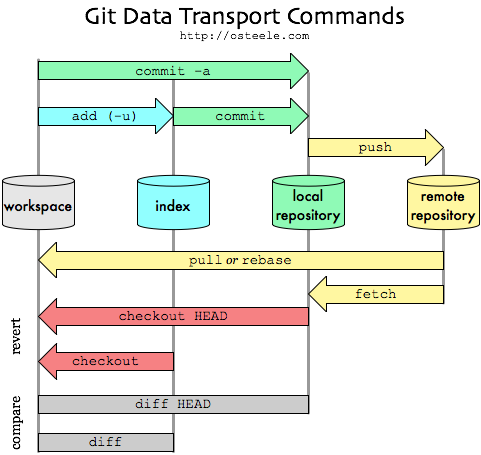
\includegraphics[width=.6\textwidth]{git.png}
	\end{center}

Keep in mind, the main mantra is, ``commit often, comment always''!

  \begin{center}
		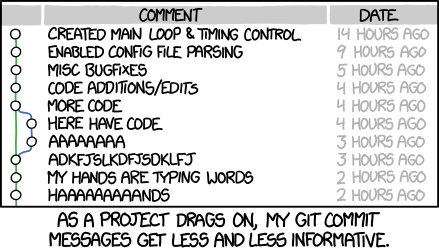
\includegraphics[width=.6\textwidth]{git_xkcd.png}
	\end{center}
	 
\section{Ignoring Files}

You will have some files you don't want to track (log files, temporary 
files, executables, etc). You can ignore entire classes of files with 
{\tt .gitignore} (be in your {\tt CMEECourseWork}!):

\begin{lstlisting}
$ echo -e "*~ \n*.tmp" > .gitignore

$ cat .gitignore
*~
*.tmp

$ git add .gitignore

$ touch temporary.tmp

$ git add *
The following paths are ignored by one of your .gitignore 
files:
temporary.tmp
Use -f if you really want to add them.
fatal: no files added
\end{lstlisting}

You can also create a global gitignore file that lists rules for files 
to be ignored in every Git repository on your computer:  
\url{https://help.github.com/articles/ignoring-files/} 

\subsection{Dealing with binary files}

A binary file is computer-readable but not human-readable, that 
is, it cannot be read by opening them in a text viewer. Examples of 
binary files include compiled executables, zip files, images, word 
documents  and videos. In contrast, text files are stored in a form (usually ASCII) 
that is human-readable by opening in a suitable text reader (e.g., 
geany, gedit). Without some git extensions and configurations (coming up 
next), binary files cannot be properly version-controlled because each version of
the entire file is saved {\it as is} in a hidden directory in the repository ({\tt .git}).

However, with some more effort, git can be made to work for binary formats like *.docx or image formats 
such as *.jpeg, but it is harder to compare versions; have a look at 
\url{https://git-scm.com/docs/gitattributes} and 
\url{https://git-scm.com/book/en/v2/Customizing-Git-Git-Attributes}\footnote{There you will find the following phrase: ``...one of the most annoying problems known to humanity: version-controlling Microsoft Word documents.'' . LOL!} 

Also see: \url{https://opensource.com/life/16/8/how-manage-binary-blobs-git-part-7}
  
\subsection{Dealing with large files}

As such, git was designed for version control of workflows and software 
projects, {\it not} large files (say, >100mb) (which may be plain-text 
or binary). Binary files are particularly problematic because each version of
the file is saved {\it as is} in \texttt{.git}, when you have a large 
number of versions it means that there
are the same number of binary files in the hidden directory (for example
100 $\times$ >100mb files!). 

In this course at least, you should not try to keep large files 
(especially binary files under version control). You will run into this 
problem in the GIS week (where you will have to handle and store large 
raster image files) in particular \footnote{None of the computing weeks 
assessments will require you to use such large files anyway}. We 
suggest that you include files larger than some size in your 
{\tt .gitignore}.  For example, you can use the following bash command: 
\begin{lstlisting}
find . -size +100M | cat >> .gitignore	
\end{lstlisting}
The 100M means 100 mb -- you can reset it to whatever you want.  

You may also explore alternatives such as {\tt git-annex} 
(e.g., see \url{https://git-annex.branchable.com/}), and {\tt git-lfs} 
(e.g., see \url{https://www.atlassian.com/git/tutorials/git-lfs}).   

\section{Removing files}

To remove a file (i.e. stop version controlling it) use {\tt git rm}:

\begin{lstlisting} 
$ echo "Text in a file to remove" > FileToRem.txt

$ git add FileToRem.txt

$ git commit -am "added a new file that we'll remove later"
master 5df9e96 added a new file that we'll remove later
 1 files changed, 1 insertions(+), 0 deletions(-)
 create mode 100644 FileToRem.txt

$ git rm FileToRem.txt
rm 'FileToRem.txt'

$ git commit -am "removed the file"
master b9f0b1a removed the file
 1 files changed, 0 insertions(+), 1 deletions(-)
 delete mode 100644 FileToRem.txt
\end{lstlisting}
  
I typically just do all my stuff and then just use {\tt git add -A}  

\section{Accessing history of the repository}

To see particular changes introduced, read the repo's log :

\begin{lstlisting} 
$ git log
commit 08b5c1c78c8181d4606d37594681fdcfca3149ec
Author: Your Name <your.login@imperial.ac.uk>
Date:   Wed Oct 8 16:41:51 2014 -0500

    removed the file

commit 13f701775bce71998abe4dd1c48a4df8ed76c08b
Author: Your Name <your.login@imperial.ac.uk>
Date:   Wed Oct 5 16:41:16 2015 -0500

    added a new file that we'll remove later

commit a228dd3d5b1921ef18c5efd926ef11ca47306ed5
Author: Your Name <your.login@imperial.ac.uk>
Date:   Wed Oct 5 10:03:40 2015 -0500

    Added README file
\end{lstlisting}

For a more detailed version, add {\tt -p} at the end.
  
\section{Reverting to a previous version}

If things go horribly wrong with new changes, you can revert to the 
previous, ``pristine'' state:

\begin{lstlisting} 
$ git reset --hard
$ git commit -am "returned to previous state" #Note I used -am here
\end{lstlisting}

If instead you want to move back in time (temporarily), first find the 
``hash'' for the commit you want to revert to, and then check-out:

\begin{lstlisting} 
$ git status
# On branch master
nothing to commit (working directory clean)

$ git log
commit c797824c9acbc59767a3931473aa3c53b6834aae
Author: Your Name <your.login@imperial.ac.uk>
Date:   Wed Aug 22 16:59:02 2014 -0500
.
.
.

$ git checkout c79782
\end{lstlisting}

Now you can play around. However, if you commit changes, you create a 
``branch'' (git plays safe!). To go back to the future, type {\tt git 
checkout master}

\section{Branching}

Imagine you want to try something out, but you're not sure it will work 
well. For example, say you want to rewrite the Introduction of your 
paper, using a different angle, or you want to see whether switching to 
a library for a piece of code improves speed. What you then need is 
branching, which creates a project copy in which you can experiment:

\begin{lstlisting} 
$ git branch anexperiment

$ git branch
  anexperiment
* master

$ git checkout anexperiment 
Switched to branch 'anexperiment'

$ git branch 
* anexperiment
  master

$ echo "Do I like this better?" >> README.txt 

$ git commit -am "Testing experimental branch"
[anexperiment 9f17dc1] Testing experimental branch
 1 files changed, 2 insertions(+), 0 deletions(-)
\end{lstlisting}
 
If you decide to merge the new branch after modifying it:

\begin{lstlisting} 
$ git checkout master

$ git merge anexperiment
Updating 08b5c1c..9f17dc1
Fast-forward
 README.txt |    2 ++
 1 files changed, 2 insertions(+), 0 deletions(-)

$ cat README.txt 
My CMEE 2015-16 Coursework Repository
Do I like this better?
\end{lstlisting}

If there are no conflicts (i.e., some files that you changed also
changed in the master in the meantime), you are done, and you can
delete the branch:

\begin{lstlisting} 
$ git branch -d anexperiment
Deleted branch anexperiment (was 9f17dc1).
\end{lstlisting}

If instead you are not satisfied with the result, and you want to
abandon the branch:
\begin{lstlisting} 
$ git branch -D anexperiment
\end{lstlisting}

When you want to test something out, always branch! Reverting changes, 
especially in code, is typically painful. Merging can be tricky, 
especially if multiple people have simultaneously worked on a 
particular document. In the worst-case scenario, you may want to delete 
the local copy and re-clone the remote repository.

\begin{center}
	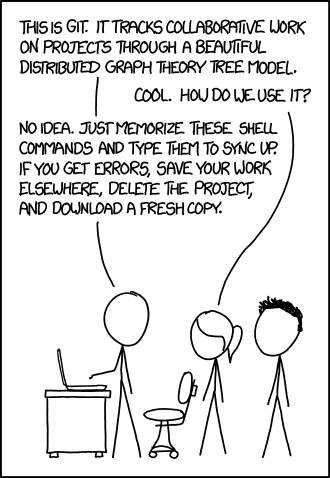
\includegraphics[width=.4\textwidth]{git_xkcd_1.png}
\end{center}
	
\section{Running git commands on a different directory}

Since {\tt git} version 1.8.5, you can run git directly on a 
different directory than the current one using absolute or relative 
paths. For example, using a relative path, you can do:
\begin{lstlisting}
git -C ../SomeDir/ status
\end{lstlisting}

\section{Running git commands on multiple repositories at once}
For git pulling in multiple subdirectories (each a separate 
repository):

\begin{lstlisting}
	$ find . -mindepth 1 -maxdepth 1 -type d -print -exec git -C {} pull \;
\end{lstlisting} 

Breaking down these commands one by one,

{\tt find .} searches the current directory\\
{\tt -type d} to find directories, not files\\
{\tt -mindepth 1} for setting min search depth to one sub-directory\\
{\tt -maxdepth 1} for setting max search depth to one sub-directory\\
{\tt -exec git -C \{\} pull $\textbackslash$ } runs a custom git command for every git repo found\\

\subsection[Practical]{Practicals}
  \begin{enumerate} \itemsep10pt
		\item The only practical submission for {\tt git} is the {\tt 
		.gitgnore} and overall git repository {\tt readme} file --- make 
		sure these in your coursework repository. 
		
		And of course, if you haven't gotten git with bitbucket 
		going, you won't be able to submit any of your practicals anyway!  
   
   \end{enumerate}


\section{Practical wrap-up}
   
  \begin{compactitem}

\item Invite me (s.pawar@imperial.ac.uk) to your {\tt CMEECourseWork} repository

\item The {\tt CMEEMasteRepo} will contain data and code files for 
upcoming practicals

\item You will clone {\tt CMEEMasteRepo} using {git clone 
git@bitbucket.org:mhasoba/cmee2015masterepo.git}

 \item You will thereafter {\tt git pull} {\tt CMEEMasteRepo}

\item You will {\tt git pull} inside {\tt CMEEMasteRepo} thereafter 
(always use {\tt git status} first)

\item {\tt cp} files from {\tt CMEEMasteRepo} to your {\tt 
CMEECourseWork} as and when needed --- don't work in the amster repo, 
as you will lose your work when I next update it! 

\end{compactitem}

\section{Readings \& Resources}

There is a wealth of information on {\tt git} out there - just google it!

\begin{compactitem}

\item Excellent book on Git: \url{http://git-scm.com/book}
\item Also, \url{https://www.atlassian.com/git/}
\item A git tutorial: \url{https://try.github.io}

\end{compactitem}

\chapter{Using \LaTeX~for scientific documents}
\label{chap:latex}

\section{What's \LaTeX?} 

In your research, you will produce papers, reports and -- very 
importantly -- your thesis. These documents can be written using a 
WYSIWYG (What You See Is What You Get) editor (e.g., Word). However, an 
alternative especially suited for scientific publications is \LaTeX. In 
\LaTeX, the document is simply a text file ({\tt .tex}). Text 
formatting is using markups (like HTML). The file is then ``compiled'' 
(like source code of a programming language) into a file -- typically 
{\tt .pdf}. 

\section{Why \LaTeX?}

\begin{compactitem}
  \item The input is a small, portable text file
  \item \LaTeX~compilers are freely available for all OS'
  \item Exactly the same result on any computer (not true for Word)
  \item \LaTeX~produces beautiful, professional looking docs (e.g., like 
this one!)
  \item Mathematical formulas (esp complex ones) are easy to write
  \item \LaTeX~is very stable -- current version basically same since 1994! 
(9 major versions of MS Word since 1994 -- with compatibility issues)
    \item \LaTeX~is free!  
    \item Many journals provide \LaTeX~templates, making formatting quicker 
    \item Bibliographies are a breeze and work with Mendeley and Zotero
    \item Plenty of online support available -- your question has probably 
already been answered
    \item You can integrate \LaTeX~into a workflow to auto-generate lengthy 
and complex documents (like your thesis).  
\end{compactitem}

\begin{center}	
	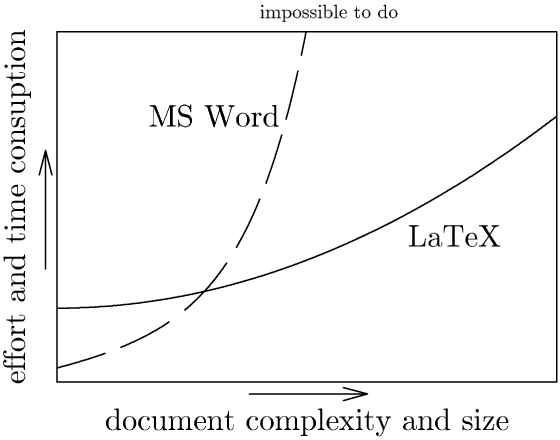
\includegraphics[width=.4\textwidth]{miktex.png}
\end{center}

\subsection{Limitations of \LaTeX}

\begin{compactitem}\itemsep10pt
  \item It has a steeper learning curve.
  
  \item Can be difficult to manage revisions with multiple authors -- 
especially if they don't use \LaTeX! (I have a dark secret)
    
  \item Typesetting tables can be a bit complex.

    \item Images and floats don't jump like Word, but if you don't use the 
right package, they can be difficult to place where you want! 

  \end{compactitem}

\section{Installing \LaTeX}
 
\begin{lstlisting} 
sudo apt-get install texlive-full texlive-fonts-recommended 
latex-beamer texlive-pictures texlive-latex-extra imagemagick       
\end{lstlisting}

We will use a text editor in this lecture, but you can use one of a 
number of WYSIWYG frontends (e.g., {\tt Lyx}, {\tt TeXmacs}), as well 
as GUI's ({\tt texmaker}, {\tt Gummi}, {\tt TeXShop}, etc). Overleaf (\url{https://www.overleaf.com/})
(now merged with Sharelatex) is also very good (and works with git), especially for 
collaborating with non \LaTeX~-ers (your university may have a blanket 
license for the pro version).  

\section{A first \LaTeX~example}

\begin{compactitem}[$\quad\star$]\itemsep4pt{}
  \item Open geany and type the following in a file
	{\tt Week1/Code/FirstExample.tex}:
\end{compactitem}

\lstinputlisting{Practicals/Code/FirstExample.tex}

Now, let's get a citation for Einstein's paper:

\begin{compactitem}[$\quad\star$]\itemsep4pt{}
\item In Google Scholar, go to ``settings'' (upper right corner) and choose
BibTeX as bibliography manager. 
  \item Now type ``does the energy of a body einstein 1905''
  \item The paper should be the one on the top.
  \item Click `` Import into BibTeX'' should show the following text, that you
will save in the file {\tt FirstBiblio.bib} (in the same directory as
{\tt FirstExample.tex})
{\tiny \lstinputlisting{Practicals/Code/FirstBiblio.bib}}
  \end{compactitem}

Now we can create a {\tt .pdf} of the article. 
\begin{compactitem}[$\quad\star$]\itemsep4pt{}
  \item In the terminal type (are you the right directory?!):
  \end{compactitem}

\begin{lstlisting}
$ pdflatex FirstExample.tex
$ pdflatex FirstExample.tex
$ bibtex FirstExample
$ pdflatex FirstExample.tex
$ pdflatex FirstExample.tex
\end{lstlisting}

This should produce the file {\tt FirstExample.pdf}:
    
\begin{center}
\setlength\fboxsep{0pt}
\setlength\fboxrule{0.5pt}
\fbox{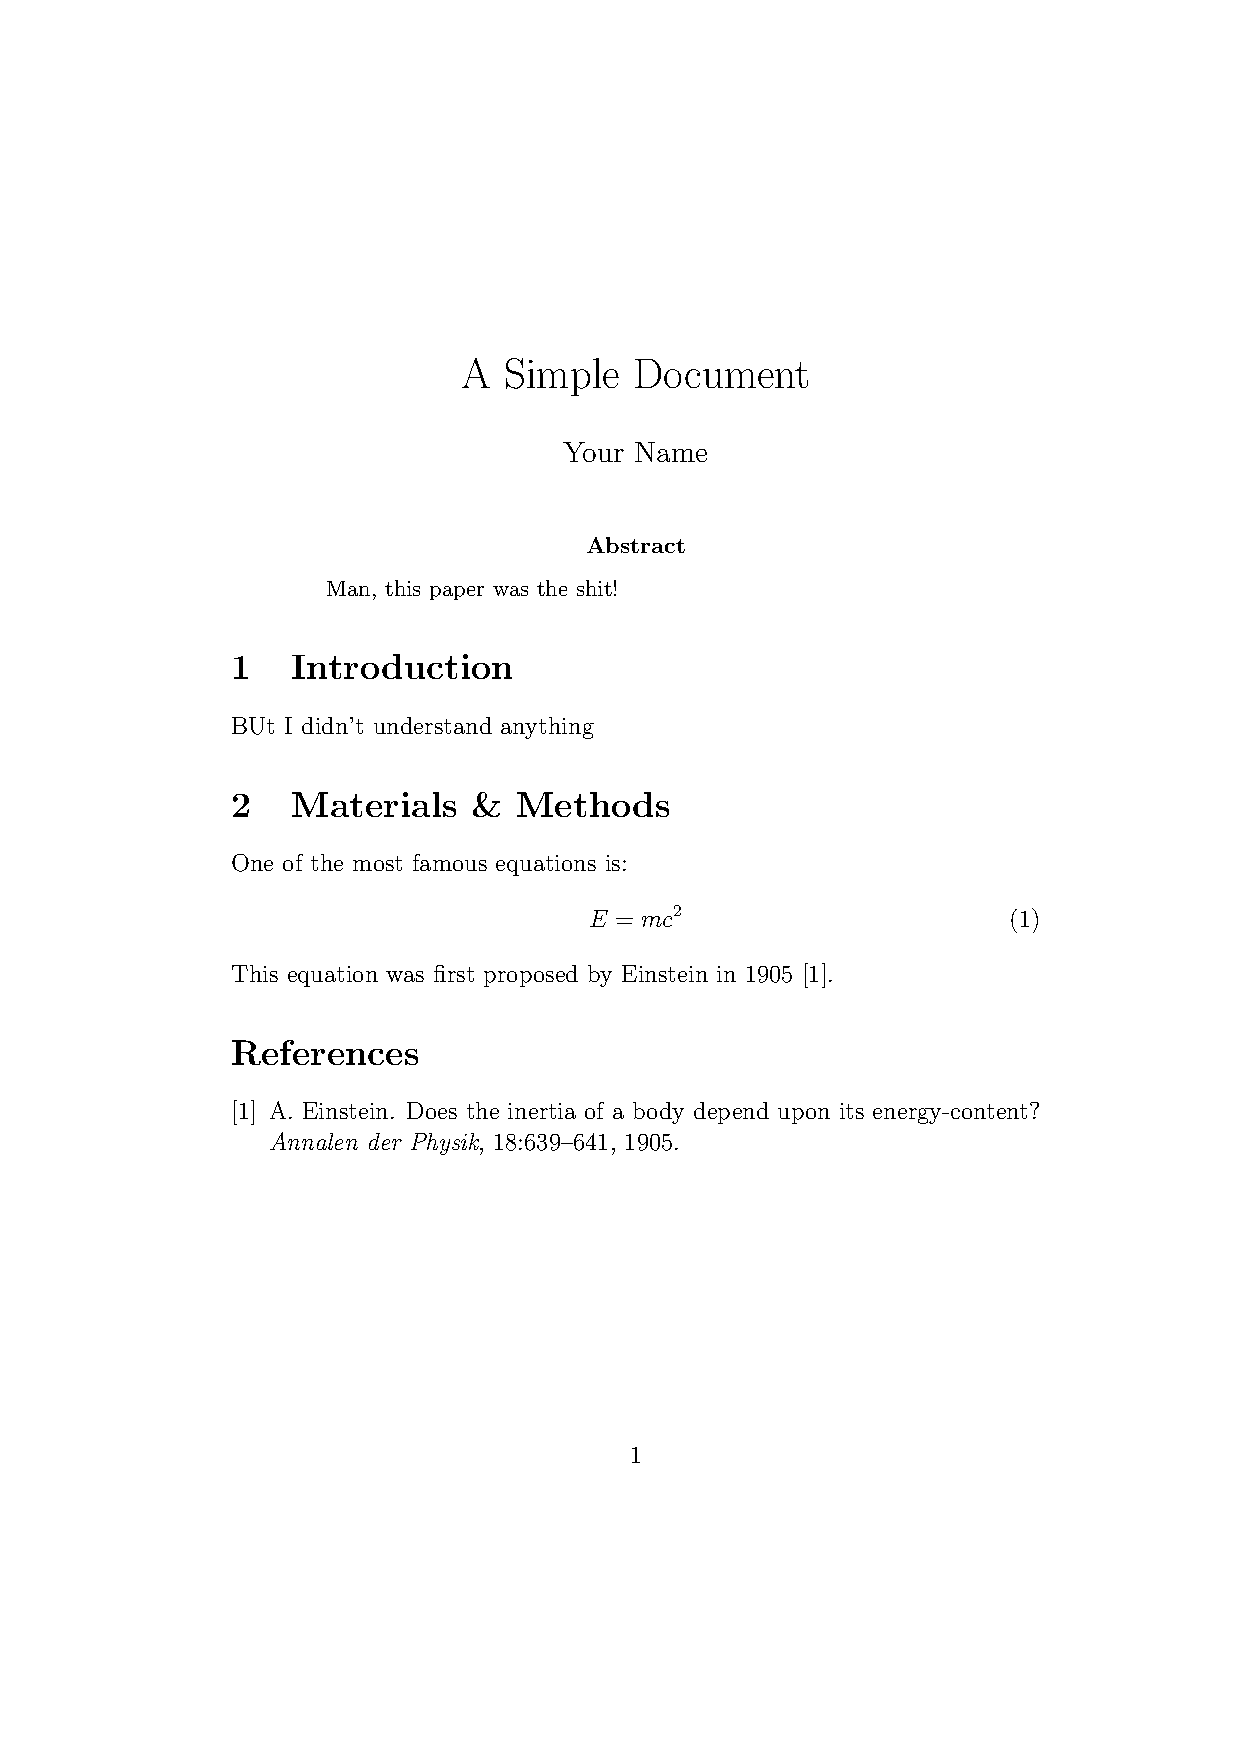
\includegraphics[width = 0.5\linewidth]{FirstExample.pdf}}
\end{center}

\subsection{A bash script to compile \LaTeX}

You can of course write a useful little bash script to compile latex 
with bibtex! 

Type the following script and call it {\tt CompileLaTeX.sh} (you know 
where to put it!):

\lstinputlisting[language=bash]{Practicals/Code/CompileLaTeX.sh}

How do you run this script? The same as your previous bash scripts, so 
\begin{lstlisting}	
$ bash CompileLaTeX.sh FirstExample
\end{lstlisting}

Why have I not written the {\tt *.tex} extension of {\tt FirstExample} 
in the command above?  

\section{A brief \LaTeX~tour}

\begin{compactitem}\itemsep12pt
\item Spaces, new lines and special characters:

\begin{compactitem} \setlength{\itemindent}{-1em}\itemsep2pt
  \item Several spaces in your text editor are treated as one space in the
typeset document
  \item Several empty lines are treated as one empty line
  \item One empty line defines a new paragraph
  \item Some characters are ``special'':\# \$ \% \^{} \& \_ \{ \}
\~{} \textbackslash. 
  \item To type these special characters, you have to add a ``backslash'' in
front, e.g., \textbackslash\$ produces \$.
\end{compactitem}

\item Document structure:

\begin{compactitem} \setlength{\itemindent}{-1em}\itemsep2pt
  \item Each \LaTeX~command starts with \textbackslash (e.g., to get \LaTeX,
you need {\tt \textbackslash{LaTeX}}
  \item The first command is always {\tt \textbackslash{documentclass}} defining
the type of document (e.g., {\tt article, book, report, letter}).
  \item You can set several options. For example, to set size of text to 10
points and the letter paper size: {\tt
\textbackslash{documentclass[10pt,letterpaper]\{article\}}}.

\end{compactitem}

  \item After having declared the type of document, you can specify packages
    you want to use. The most useful are:

\begin{compactitem}
  \item{\tt \textbackslash{usepackage\{color\}}}: use colors for text in your
document.
  \item{\tt \textbackslash{usepackage\{amsmath,amssymb\}}}: American
Mathematical Society formats and commands for typesetting mathematics. 
  \item{\tt \textbackslash{usepackage\{fancyhdr\}}}: fancy headers and footers. 
  \item{\tt \textbackslash{usepackage\{graphicx\}}}: include figures in pdf, ps,
eps, gif and jpeg.
  \item{\tt \textbackslash{usepackage\{listings\}}}: typeset source code for
various programming languages.
  \item{\tt \textbackslash{usepackage\{rotating\}}}: rotate tables and figures.
  \item{\tt \textbackslash{usepackage\{lineno\}}}: line numbers.
\end{compactitem}

\item Once you select the packages, you can start your document with {\tt
\textbackslash{begin\{document\}}}, and end it with {\tt
\textbackslash{end\{document\}}}.

\end{compactitem}

\section{\LaTeX~templates}

There a lots of useful \LaTeX templates out there. As an example of 
structure of a document, take the article template provided by the 
journal PNAS:

{\tiny \lstinputlisting{Practicals/Code/PnasExample.tex}}

I have added some templates in the {\tt CMEEMasteRepo} that you should 
have a look and play around with

\section{Typesetting math}

There are two ways to display math 

 \begin{enumerate}

  \item First, one can produce inline mathematics (i.e., within the text).
    \item Second, one can produce stand-alone, numbered equations and formulae.
    
   \end{enumerate}
   
For inline math, the ``dollar'' sign flanks the math to be typeset. For 
example, the code:
\begin{lstlisting}
$\int_0^1 p^x (1-p)^y dp$
\end{lstlisting}

Becomes $\int_0^1 p^x (1-p)^y dp$

For numbered equations (almost always a great idea), \LaTeX~provides 
the {\tt equation} environment:

\begin{lstlisting}

\begin{equation}
\int_0^1 \left(\ln \left( \frac{1}{x} \right) 
\right)^y dx = y!
\end{equation}

\end{lstlisting}

Becomes:
\begin{equation}
\int_0^1 \left(\ln \left( \frac{1}{x} \right) \right)^y dx = y!
\end{equation}

\section{A few more tips}

The following tips might prove handy:

\begin{compactitem}
\item \LaTeX~has a full set of symbols and operators (plenty of lists online)
\item Long documents can be split into separate {\tt.tex} documents and
combined using {\tt input}
\item Long documents can be split into separate {\tt.tex} documents and
\item Figures can be included using the {\tt graphicx} package
\item You can use Mendeley to export and maintain {\tt .bib} files
\item You can redefine environments and commands in the preamble 
\end{compactitem}

\subsection[Practical]{Practicals}
  
	Test {\tt CompileLaTeX.sh} with {\tt FirstExample.tex} and 
	bring it under verson control under{\tt CMEECourseWork/Week1} in 
	your repository. Make sure that {\tt CompileLaTeX.sh} will work if 
	I ran it from my computer using {\tt FirstExample.tex} as an input.

\section[Practical]{Practicals wrap-up}

Make sure you have your {\tt Week 1} directory organized 
with {\tt Data}, {\tt Sandbox} and {\tt Code} with the necessary 
files and this week's (functional!) scripts in there. Every script 
should run without errors on my computer. This includes the five 
solutions (single-line commands you came up with) in {\tt 
UnixPrac1.txt}.

\begin{center}
	\it Commit and push everything by next Wednesday 5 PM.
\end{center} 

\section{Readings \& Resources}

\begin{itemize}

\item The Visual \LaTeX~ FAQ: sometimes it is difficult to describe what you
want to do!\\
\url{http://get-software.net/info/visualFAQ/visualFAQ.pdf}

\item Myriad online resources for \LaTeX, including:\\
\url{www.http://en.wikibooks.org/wiki/LaTeX/Introduction},\\
\url{www.ctan.org/tex-archive/info/lshort/english/}\\
\url{http://ftp.uni-erlangen.de/mirrors/CTAN/info/lshort/english/lshort.pdf}
\item Beautiful presentations in \LaTeX: 
\url{http://tug.org/pracjourn/2005-2/miller/miller.pdf}
\item Bibliographies in \LaTeX: \url{http://schneider.ncifcrf.gov/latex.html}

\end{itemize}



\chapter{Basic Biological Computing in Python}
\label{chap:pythonI}

\epigraph{Science is what we understand well enough to explain to a 
computer. Art is everything else we do}{\textit{---Donald Knuth}}

{\bf Firstly, chapter \ref{chap:unix1}'s UNIX question?}
\begin{lstlisting}
find . -type f -exec ls -s {} \; | sort -n | head -10
\end{lstlisting}
What is the command doing? How has it been built (explain the components)?
% Sort and head to find the largest 10 files, including in 
% sub-directories. A faster option would be 
% find . -type f -exec ls -s {} + | sort -n | head -10
% See {\tt man find}, especially the part about the {\tt -exec option}

% Basically, -exec runs a command ({\tt ls -s} in this case) on each of 
% the files found, {} is replaced with the name of each file found, 
% and the find command is terminated by \;

\section{Outline of the {\tt python} module} 

The {\tt python} module is geared towards teaching you scientific 
programming in biology using this modern, and for good reason, 
immensely popular language. The components of this module across all 
the chapters (Basic, Advanced, Additional topics) are: 
\begin{compactitem}
	\item Basics of {\tt python}
	\item How to write and run {\tt python} code
	\item Understand and implement ``control flows''
	\item Learning to use the {\tt ipython} environment
	\item Writing, debugging, using, and testing {\tt python} functions
	\item Learning efficient numerical programming in {\tt python}
	\item Using regular expressions in {\tt python}  
	\item Introduction to certain particularly useful {\tt python} packages
	\item Using {\tt python} for building and modifying databases
	\item Using {\tt python} to run other ``stuff'' and to patch 
	together data analysis and/or numerical simulation work flows
\end{compactitem} 

\begin{figure} \centering
	    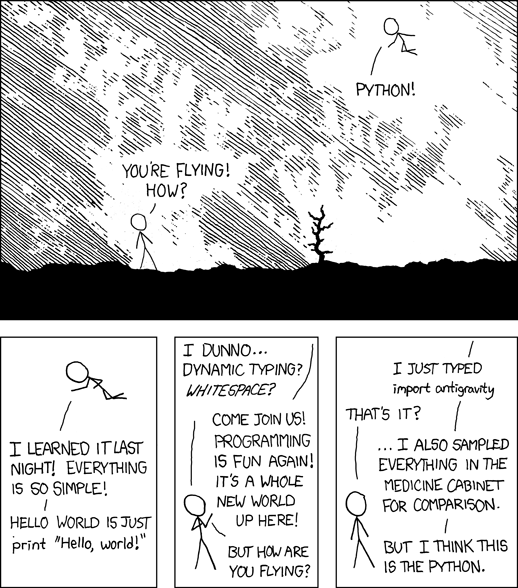
\includegraphics[width=.4\textwidth]{python.png}\\
		\url{www.xkcd.com}
	\caption{Is {\tt python} the most common answer to your daily 
	programming needs? Possibly!}
\end{figure}

\section{Why {\tt python}?}

{\tt python} was designed with readability and re-usability in mind. 
Time taken by programming + debugging + running is likely to be 
relatively lower in {\tt python} than less intuitive or cluttered 
languages (e.g., {\tt FORTRAN}, {\tt perl}). It is a pretty good 
solution if you want to  easily write readable code that is also 
reasonably efficient (computationally speaking).

\begin{figure}
	\begin{center}
    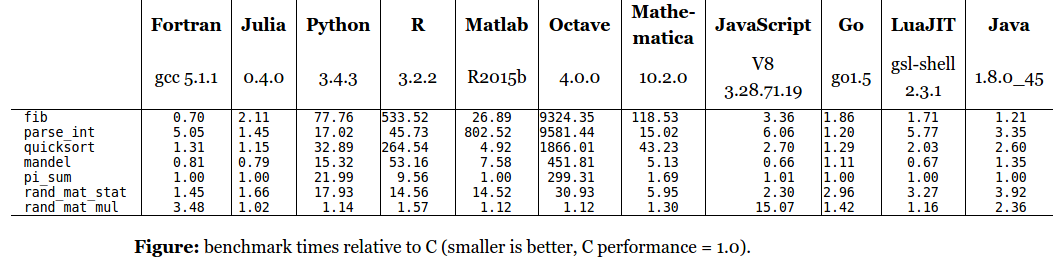
\includegraphics[width=1\textwidth]{benchmark.png}\\
		\url{http://julialang.org/}
	\end{center}
	\caption{{\tt python} is pretty fast!}
\end{figure}

\subsection{The Zen of python}
Open a terminal and type
\begin{lstlisting}
$ python -c "import this"
\end{lstlisting}

\section{Installing {\tt python}}

{\bf We will use 2.7.x, not 3.x (you can use 3.x later, if you want)}

Your Ubuntu distribution needs {\tt python}, so it will already be installed. 
However, let's install the interactive python shell {\tt ipython} which 
we will soon use.   
\begin{compactitem}[$\quad\star$]\itemsep4pt
\item On Ubuntu/Linux, open a terminal (ctrl+alt+t) and type:
\begin{lstlisting}
$ sudo apt-get install ipython python-scipy python-matplotlib
\end{lstlisting}
\end{compactitem}

\begin{tipbox}
In Linux, you can easily install python packages that come with the 
standard python distribution using the usual {\tt sudo apt-get install 
python-packagename}
\end{tipbox}
 
\section{Getting started with {\tt python}}
Open a terminal ({\tt ctrl+alt+t}) and type {\tt python} (or use the 
terminal that you just used to install {\tt ipython}). Then, try the 
following:
\begin{lstlisting}
>>> 2 + 2 # Summation; note that comments start with #
4

>>> 2 * 2 # Multiplication
4

>>> 2 / 2 # Integer division
1

>>> 2 / 2.0 # "Float" division, note the output is float
1.0

>>> 2 / 2.
1.0

>>> 2 > 3
False

>>> 2 >= 2
True
\end{lstlisting}

What does "float" mean in the above comment? Why is it necessary to 
specify this in Python (not necessary in Python 3.x)? You will 
inevitably run into some such jargon in this chapter. The main ones you 
need to know are (you will learn more about these along the way):

\begin{tabular}{p{2.2cm} p{12cm}} 
	Workspace & The state of the ``environment'' of your current python 
	{\it session}, including all variables, functions, objects, etc. \\ 
	Variable & A named number, text string, boolean ({\tt True} or {\tt False}), or data 
	structure that can change (more on variable	and data types later)\\
	Function &  A computer procedure or routine that returns some value(s), 
	and which can be used again and again \\
	Module & {\it Variables} and {\it functions} packaged into a single 
	set of programs that can be invoked as a command (potentially with sub-commands)  \\
	Class &  Also, variables and functions packaged into a single set of programs 
	that that can be invoked as a command (potentially with sub-commands), but unlike modules, you can spawn many 
	copies of a class within a python session or program\\
	Object & A particular instance of a class (every object belongs to a 
	class) that is created in  a session and eventually destroyed; 
	pretty much everything in your workspace is an object in python!  \\
\end{tabular}
This Module vs. Class vs. Object business is confusing. These 
constructs are created to make an (object-oriented) programming 
language like {\tt python} more flexible and user friendly (though it 
might not seem so to you currently!). In practice, at least for your 
current purposes, you will not build python classes yourself much, 
typically working with modules. More on all this later. Also, have a 
look at \url{https://learnpythonthehardway.org/book/ex40.html}

\subsection{\tt ipython}
We will now immediately switch to the {\tt i}nteractive {\tt python} 
shell, {\tt ipython} that you installed above. 

OK, now let's continue learning python using {\tt ipython}. 
\begin{compactitem}[$\quad\star$]\itemsep4pt{}
\item Type {\tt ctrl+D} in the terminal at the python prompt: this will 
exit you from the python shell and you will see the bash prompt again. 
\item Now type {\tt ipython}  
\end{compactitem}

You should now see (after some text):

\begin{lstlisting}
In [ ]: 
\end{lstlisting}
(I have deleted the prompt numbering {\tt [1]}, {\tt [2]}, etc to avoid 
confusion). This is the {\tt i}nteractive {\tt python} shell (or, "{\tt ipython}"). 
This shell has many advantages over the bare-bones, non-interactive 
python shell with the $>>>$ prompt. For example, as in the bash shell, 
{\tt TAB} leads to auto-completion of a command or file name (try it).

\subsection{Magic commands}
IPython also has ``magic commands'' (start with \%; e.g., {\tt \%run}). 
Some useful magic commands:

\begin{tabular}{p{2.5cm} p{10cm}} 
	{\tt \%who} & Shows current namespace (all variables, modules and 
	functions)\\
	{\tt \%whos} & Also display the type of each variable; typing {\tt 
	\%whos function} only displays functions etc.\\
  {\tt \%pwd} & Print working directory\\
	{\tt \%history} & Print recent commands\\
\end{tabular}

Try any of these now!
 
\subsection{Determining an object's type}
Another useful IPython feature is the question mark, which can be used 
to find what a particular Python object is, including variables you 
created. For example, try: 
\begin{lstlisting}
In [1]: a = 1

In [2]: ?a
Type:        int
String form: 1
Docstring:
int(x=0) -> int or long
int(x, base=10) -> int or long

Convert a number or string to an integer, or return 0 if no arguments
are given.  If x is floating point, the conversion truncates towards zero.
If x is outside the integer range, the function returns a long instead.

If x is not a number or if base is given, then x must be a string or
Unicode object representing an integer literal in the given base.  The
literal can be preceded by '+' or '-' and be surrounded by whitespace.
The base defaults to 10.  Valid bases are 0 and 2-36.  Base 0 means to
interpret the base from the string as an integer literal.
>>> int('0b100', base=0)
4
\end{lstlisting}

\begin{tipbox}
You can configure ipython's environment and behavior by editing 
the {\tt ipython\_config.py} file:
\begin{lstlisting}
$ geany ~/.config/ipython/profile_default/ipython_config.py &
\end{lstlisting}
This file does not inititally exist, but you can create it by running  
{\tt ipython profile create} in a bash terminal (try it now). 

Now you can configure ipython. For example, If you don't like the blue 
{\tt ipython} prompt, you can type {\tt \%colors linux} (once inside 
the shell). If you want to make this color the default, then edit {\tt 
ipython\_config.py} --- search for ``Set the color scheme'' in the 
file. 
\end{tipbox}
\section{Python variables}

Now, let's continue our python intro. We will first learn about the {\tt 
python} variable types that were mentioned above. The types are:

\begin{lstlisting}
In [ ]: a = 2 #integer

In [ ]: ?a
Type:        int
String form: 2
Docstring:
int(x=0) -> int or long
int(x, base=10) -> int or long

Convert a number or string to an integer, or return 0 if no arguments
are given.  If x is floating point, the conversion truncates towards zero.
If x is outside the integer range, the function returns a long instead.

If x is not a number or if base is given, then x must be a string or
Unicode object representing an integer literal in the given base.  The
literal can be preceded by '+' or '-' and be surrounded by whitespace.
The base defaults to 10.  Valid bases are 0 and 2-36.  Base 0 means to
interpret the base from the string as an integer literal.
>>> int('0b100', base=0)
4

In [ ]: a = 2. #Float

In [ ]: ?a
Type:        float
String form: 2.0
Docstring:
float(x) -> floating point number

Convert a string or number to a floating point number, if possible.

In [ ]: a = "Two" #String

In [ ]: ?a
Type:        str
String form: Two
Length:      3
Docstring:
str(object='') -> string

Return a nice string representation of the object.
If the argument is a string, the return value is the same object.

In [10]: a = True #Boolean

In [11]: ?a
Type:        bool
String form: True
Docstring:
bool(x) -> bool

Returns True when the argument x is true, False otherwise.
The builtins True and False are the only two instances of the class bool.
The class bool is a subclass of the class int, and cannot be subclassed.
\end{lstlisting}

Thus, {\tt python} has integer, float (real numbers, with different 
precision levels) and string variables.

\subsection{{\tt python} operators}
Here are are the operators in python that you can use on variables:

\begin{tabular}{p{2cm} p{10cm}} 
  {\tt +} & Addition\\
  {\tt -} & Subtraction\\
  {\tt *} & Multiplication\\
  {\tt /} & Division\\
  {\tt **} & Power\\
  {\tt \%} & Modulo\\
  {\tt //} & Integer division\\
  {\tt ==} & Equals\\
  {\tt !=} & Differs\\
  {\tt $>$} & Greater\\
  {\tt $>$=} & Greater or equal\\
  {\tt \&, and} & Logical and\\
  {\tt $\vert$, or} & Logical or\\
  {\tt !, not} & Logical not\\	
\end{tabular}

\subsection{Assigning and manipulating variables}

\begin{lstlisting}
 In []: 2 == 2
Out []: True

 In []: 2 != 2
Out []: False

 In []: 3 / 2
Out []: 1

 In []: 3 / 2.
Out []: 1.5

 In []: 'hola, ' + 'mi llamo Samraat' #why not two languages at the same
time?! 
Out []: 'hola, mi llamo Samraat'

In []: x = 5

 In []: x + 3
Out []: 8

 In []: y = 8

 In []: x + y
Out []: 13

 In []: x = 'My string'

 In []: x + ' now has more stuff'
Out []: 'My string now has more stuff'

 In []: x + y
Out []: TypeError: cannot concatenate 'str' and 'int' objects
\end{lstlisting}

OK, so concatenating string and numeric (integer in this case) 
variables doesn't work.  No problem, we can convert from one type to 
another:

\begin{lstlisting}
 In []: x + str(y)
Out []: 'My string8'

 In []: z = '88'

 In []: x + z
Out []: 'My string88'

 In []: y + int(z)
Out []: 96
 \end{lstlisting} 

\begin{tipbox}
In {\tt python}, the type of a variable is determined when the  program 
or command is running (dynamic typing) (like {\tt R}, unlike {\tt C} or 
{\tt FORTRAN}). This is convenient, but can make programs slow. More 
on efficient computing later.
\end{tipbox}

\section{{\tt python} data types and data structures}

{\tt python} number or string variables (or both) can be stored and manipulated in:
\begin{compactitem} \itemsep4pt
 \item  {\bf List}: most versatile, can contain compound data, ``mutable'',
enclosed in brackets, [ ]
 \item  {\bf Tuple}: like a list, but ``immutable'' --- like a read only list,
enclosed in parentheses,  ( ) 
 \item  {\bf Dictionary}: a kind of ``hash table'' of key-value pairs enclosed
by curly braces, \{ \} --- key can be number or string, values can be any
object! (well OK, a python object)
 \item  {\bf numpy arrays}: Fast, compact, convenient for numerical computing --- more on this later!
\end{compactitem}

\subsection{Lists}

\begin{lstlisting} 
 In []: MyList = [3,2.44,'green',True]

 In []: MyList[1]
Out []: 2.44

 In []: MyList[0] # NOTE: FIRST ELEMENT -> 0
Out []: 3

 In []: MyList[4]
Out []: IndexError: list index out of range

 In []: MyList[2] = 'blue'

 In []: MyList
Out []: [3, 2.44, 'blue', True]

 In []: MyList[0] = 'blue'

 In []: MyList
Out []: ['blue', 2.44, 'blue', True]

 In []: MyList.append('a new item') # NOTE: ".append"!

 In []: MyList
Out []: ['blue', 2.44, 'blue', True, 'a new item']

 In []: MyList.sort() # NOTE: suffix a ".", hit tab, and wonder!

 In []: MyList
Out []: [True, 2.44, 'a new item', 'blue', 'blue']
\end{lstlisting}

In the above commands, notice that {\tt python} "indexing" starts at 0, 
not 1!  

\subsection{Tuples}

\begin{lstlisting} 
 In []: FoodWeb=[('a','b'),('a','c'),('b','c'),('c','c')]

 In []: FoodWeb[0]
Out []: ('a', 'b')

 In []: FoodWeb[0][0]
Out []: 'a'

 In []: FoodWeb[0][0] = "bbb"  # NOTE: tuples are "immutable"
      TypeError: 'tuple' object does not support item assignment

 In []: FoodWeb[0] = ("bbb","ccc")

 In []: FoodWeb[0]
Out []: ('bbb', 'ccc')
\end{lstlisting} 

Note that tuples are "immutable"; that is, a particular pair or 
sequence of strings or numbers cannot be modified after it is created.

In the above example, why assign these food web data to a list of 
tuples and not a list of lists? --- because we want to maintain the 
species associations, no matter what --- they are sacrosanct! 

Tuples contain immutable sequences, but you can append to them:

\begin{lstlisting} 
 In []: a = (1, 2, [])
 
 In []: a[2].append(1000)
 
 In []: a
Out []: (1, 2, [1000])
\end{lstlisting}

\subsection{Sets}
You can convert a list to an immutable ``set'' --- an unordered 
collection with no duplicate elements. Once you create a set you
can perform set operations on it:

\begin{lstlisting} 
 In []: a = [5,6,7,7,7,8,9,9]

 In []: b = set(a)

 In []: b
Out []: set([8, 9, 5, 6, 7])

 In []: c = set([3,4,5,6])

 In []: b & c
Out []: set([5, 6])

 In []: b | c
Out []: set([3, 4, 5, 6, 7, 8, 9])

 In []: list(b | c) # set to list
Out []: [3, 4, 5, 6, 7, 8, 9]

\end{lstlisting}

The key set operations in {\tt python} are: 

\begin{tabular}{p{2.5cm} p{10cm}} 
	{\tt a - b } & a.difference(b)\\
	{\tt a $<=$ b} & a.issubset(b)\\
	{\tt a $>=$ b} & b.issubset(a)\\
	{\tt a \& b} & a.intersection(b)\\
	{\tt a $\vert$ b} & a.union(b)\\
\end{tabular}

\subsection{Dictionaries}

A set of values (any {\tt python} object) indexed by keys (string or 
number), a bit like {\tt R} lists.

\begin{lstlisting} 
In []: GenomeSize = {'Homo sapiens': 3200.0, 'Escherichia coli': 4.6,
'Arabidopsis thaliana': 157.0}

 In []: GenomeSize
Out []: 
{'Arabidopsis thaliana': 157.0,
  'Escherichia coli': 4.6,
  'Homo sapiens': 3200.0}

 In []: GenomeSize['Arabidopsis thaliana']
Out []: 157.0

 In []: GenomeSize['Saccharomyces cerevisiae'] = 12.1

 In []: GenomeSize
Out []: 
{'Arabidopsis thaliana': 157.0,
'Escherichia coli': 4.6,
'Homo sapiens': 3200.0,
'Saccharomyces cerevisiae': 12.1}

 In []: GenomeSize['Escherichia coli'] = 4.6  # ALREADY IN DICTIONARY!

 In []: GenomeSize
Out []: 
{'Arabidopsis thaliana': 157.0,
 'Escherichia coli': 4.6,
 'Homo sapiens': 3200.0,
 'Saccharomyces cerevisiae': 12.1}

 In []: GenomeSize['Homo sapiens'] = 3201.1

 In []: GenomeSize
Out []: 
{'Arabidopsis thaliana': 157.0,
 'Escherichia coli': 4.6,
 'Homo sapiens': 3201.1,
 'Saccharomyces cerevisiae': 12.1} 
\end{lstlisting}

So, in summary, 
\begin{compactitem} \itemsep10pt
	\item  If your elements/data are unordered and indexed by numbers use 
	{\bf lists}
  \item  If they are ordered sequences use a {\bf tuple} 
	\item  If you want to perform set operations on them, use a {\bf set}
	\item  If they are unordered and indexed by keys (e.g., names), use a 
	{\bf dictionary}
\end{compactitem}

{\it But why not use dictionaries for everything?} -- because it can 
slow down your code!

\subsection{Copying mutable objects}

Copying mutable objects can be tricky. Try this:

\lstinputlisting{Practicals/Code/deepcopy.py}

So, you need to employ {\tt deepcopy} to really copy an existing object 
or variable and assign a new name to the copy. 

\subsection{{\tt python} with strings}

One of the things that makes python so useful and versatile, is that it 
has a powerful set of inbuilt commands to perform string manipulations. 
For example, try these: 

\lstinputlisting{Practicals/Code/exstrings.py}

\section{Writing {\tt python} code}

Now let's learn to write and run python code from a {\tt *.py} file. 
But first, some some guidelines for good code-writing practices (see
\url{python.org/dev/peps/pep-0008/}):
  \begin{compactitem} \itemsep8pt
    \item Wrap lines to be $<$80 characters long. You can use parentheses $()$
  or signal that the line continues using a ``backslash'' $\backslash$
    \item Use either 4 spaces for indentation or tabs, but not both! (I use tabs!)
    \item Separate functions using a blank line
    \item When possible, write comments on separate lines
  \end{compactitem}

Make sure you have chosen a particular indent type (space or tab) in 
{\tt geany} (or whatever IDE you are using) --- indentation is all-important 
in {\tt python}. Furthermore, 
\begin{compactitem} \itemsep4pt
    \item Use ``docstrings'' to {\bf document how to use the code}, and
      {\bf comments to explain why and how the code works}
    \item Naming conventions (bit of a mess, you'll learn as you go!):
    \begin{compactitem}
      \item {\tt \_internal\_global\_variable} (for use inside module only)
      \item {\tt a\_variable}
      \item {\tt SOME\_CONSTANT}
      \item {\tt a\_function}
			\item Never call a variable {\tt l} or {\tt O} or {\tt o}\\ {\it 
			why not?} -- you are likely to confuse it with {\tt 1} or {\tt 0}!
    \end{compactitem}
	\item Use spaces around operators and after commas:\\ 
  {\tt  a = func(x, y) + other(3, 4)} 
\end{compactitem}

\section{{\tt python} Input/Output}

Let's look at importing and exporting data.  Make a textfile called 
{\tt test.txt} in {\tt Week2/Sandbox/} with the following content 
(including the empty lines):

\begin{lstlisting}
First Line
Second Line

Third Line

Fourth Line
\end{lstlisting}

Then, type the following in {\tt Week2/Code/basic\_io.py} (note the 
indentation!):

\lstinputlisting{Practicals/Code/basic_io.py}

Note the following:

\begin{compactitem}
	\item The {\tt for line in f} is an implicit loop --- implicit 
	because stating the range of things in {\tt f} to loop over in this 
	way allows python to handle any kind of objects to loop thorugh. For 
	example, if {\tt f} was an array of numbers 1 to 10, it would loop 
	thorugh them; if {\tt f} is a file, as in the case of the script 
	above, it will loop through the lines in the file.
	
	\item {\tt is len(line.strip()) > 0} checks if the line is empty. Try 
	{\tt ?} to see what {\tt .strip()} does.	 
\end{compactitem}

The {\tt csv} package makes it easy to manipulate CSV files (get {\tt 
testcsv.csv} from {\tt CMEEMasteRepo}). Type the following script in 
{\tt Week2/Code/basic\_csv.py}
  
\lstinputlisting{Practicals/Code/basic_csv.py}

\begin{tipbox}
Now that you have seen how all-important indentation of python code is, 
you might find the {\tt ipython \%cpaste} function very handy, as it 
allows you to run fragments of code, indentation and all, directly in 
the {\tt ipython} commandline. Let's try it. Type the following code 
in a temporary file:
\begin{lstlisting}
for i in range(x):
		if i > 3: #4 spaces or 2 tabs in this case
				print i 
\end{lstlisting}
Now, assign some integer value to a variable {\tt x}: 
\begin{lstlisting}
In [ ]: x = 11
\end{lstlisting}
Then,
\begin{lstlisting}
In [ ]: %cpaste
Pasting code; enter '--' alone on the line to stop or use Ctrl-D.
:for i in range(x):
:    if i > 3: #4 spaces or 2 tabs in this case
:        print i
:--
4
5
6
7
8
9
10
\end{lstlisting}
Of course, this code is simple, so directly pasting works as well --- 
{\tt \%cpaste} is really useful when you have more complex code fragments 
you want to try out. Se haow far you have to pus direct pasting till 
you need {\tt \%cpaste}
\end{tipbox}

\subsection{Writing {\tt python} functions (or modules)}

Now let's writing proper {\tt python} functions. We will start with a 
``boilerplate'' code. Type the code below and save as {\tt 
boilerplate.py} in {\tt CMEECourseWork/Week2/Code}:

\lstinputlisting{Practicals/Code/boilerplate.py}

\subsubsection{Running your {\tt python} code}

Now {\tt cd } to the directory and run the code:
\begin{lstlisting}
$ cd ~/Documents/../CMEECourseWork/Week2/Code
$ python boilerplate.py
\end{lstlisting}

You should see "This is a boilerplate" in your terminal window. 

Alternatively, you can use ipython:
\begin{lstlisting} 
$ ipython boilerplate.py
\end{lstlisting}

You can also execute a python script file from within the {\tt ipython} 
shell with {\tt run MyScript.py}. So, enter {\tt ipython} from bash, 
and do: 
\begin{lstlisting} 
In [ ]: run boilerplate.py
\end{lstlisting}

To run the script from the native python shell, you would use {\tt 
execfile("MyScript.py")}.

\subsection{Components of the {\tt python} function}

Now let's look at the elements of your first, boilerplate code:

\subsubsection{The shebang}

Just like UNIX shell scripts, the first "shebang" line tells the 
computer where to look for python. It determines the script's ability 
to be executed like an standalone executable without typing python 
beforehand in the terminal or when double clicking it in a file 
manager (when configured properly to be an executable). It isn't 
necessary but generally put there so when someone sees the file opened 
in an editor, they immediately know what they're looking at. However, 
which shebang line you use is important. 

Here by using {\tt \#!/usr/bin/python} we are specifying the location 
to the python executable in your machine that rest of the script needs 
to be interpreted with. You may want to use {\tt \#!/usr/bin/env 
python} instead, which will prevent failure to run if the Python 
executable on some other machine or distribution isn't actually located 
at {\tt \#!/usr/bin/python}, but elsewhere.

\subsubsection{The Docstring}

Triple quotes start a ``docstring'' comment, which is meant to describe 
the operation of the script or a function/module within it. docstrings 
are considered part of the running code, while normal comments are 
stripped. Hence, you can access your docstrings at run time. It is a 
good idea to have doctrings at the start of every python script and 
module as it can provide useful information to the user and you as 
well, down the line. 

You can access the docstring(s) in a script (both 
for the overall script and the ones in each of its functions), by 
importing the function (say, {\tt my\_func}), and then typing {\tt 
help(my\_func)} in the python or ipython shell. For example, try {\tt 
import boilerplate} and then {\tt help(boilerplate)} (but you have 
to be in the python or ipython shell). 

For more info, see \url{https://www.python.org/dev/peps/pep-0257}

\subsubsection{Internal Variables}

%% What's going on here?
``{\tt \_\_}'' signal ``internal'' variables (never name your
variables so!)

\subsubsection{Function {\tt def}initions and "modules"}

{\tt def} indicates the start of a python function; all subsequent 
lines must be indented.

It's important to know that somewhat confusingly, Pythonistas 
call a file containing function {\tt def}itions's) and statements 
(e.g., assignments of constant variables) a "module". There is a 
practical reason (there's always one!) for this. You might want to use 
a particular set of python {\tt def}'s (functions) and statements 
either as a standalone function, or use it or subsets of it from other 
scripts. So in theory, every function you {\tt def}ine can be a 
sub-module usable by other scripts. 

{\it In other words, {\tt def}initions from a module can be imported 
into other modules and scripts, or into the main module itself.} 

At this juncture, you might also want to know more about a Python 
"class". Have a look at 
\url{http://learnpythonthehardway.org/book/ex40.html} --- a nice, 
intuitive tutorial that should help you understand functions vs. 
modules vs. classes in Python.

The last few lines, including the {\tt main} function/module are 
somewhat esoteric but important; more on this below.
 
\subsubsection{Why include {\tt \_\_name\_\_ == "\_\_main\_\_"} and all 
that jazz}

When you run a Python module with or without arguments, the code in the 
called module will be executed just as if you imported it, but with the 
{\tt \_\_name\_\_} set to {\tt "\_\_main\_\_"}. So adding this code 
at the end of your module,
\begin{lstlisting}
if (__name__ == "__main__"):
\end{lstlisting}
directs the {\tt python} interpreter to set the special {\tt 
\_\_name\_\_} variable to have a value "{\tt  \_\_main\_\_}", so that 
the file is usable as a script as well as an importable module. How do 
you import? Simply as (in python or ipython shell):
\begin{lstlisting}
In []: import boilerplate
\end{lstlisting}
Then type 
\begin{lstlisting}
In []: boilerplate
Out[]: <module 'boilerplate' from 'boilerplate.py'>
\end{lstlisting}

One more script to hopefully clarify this further. Type and save the 
following in a script file called {\tt using\_name.py}: 
\lstinputlisting{Practicals/Code/using_name.py}
Now run it:
\begin{lstlisting}
In []: run using_name.py
This program is being run by itself
\end{lstlisting}

Now, try:
\begin{lstlisting}
In []: import using_name
I am being imported from another module
\end{lstlisting}
	
The output {\tt I am being imported from another module} will only 
show up once. 

Also please look up \url{https://docs.python.org/2/tutorial/modules.html}

\subsubsection{What on earth is {\tt sys.argv}?}

In your boilerplate code, as any other Python code, {\tt argv} is the 
"argument variable". Such variables are necessarily very common across 
programming languages, and play an important role --- {\tt argv} is a 
variable that holds the arguments you pass to your Python script when 
you run it. {\tt sys.argv} is simply an object created by python 
using the {\tt sys} module (which you imported at the beginning of the 
script) that contains the names of the argument variables in the 
current script.

To understand this in a practical way, let's write and save 
a script called {\tt sysargv.py}: 
\lstinputlisting{Practicals/Code/sysargv.py}
Now run {\tt sysargv.py} with different numbers of arguments:
\begin{lstlisting}
run sysargv.py
run sysargv.py var1 var2
run sysargv.py 1 2 var3
\end{lstlisting}
As you can see the first variable is always the file name, and is always 
available as to the Python interpreter.

Then, the command {\tt main(argv=sys.argv)} directs the interpreter to 
pass the argument variables to the main function. Which brings us to,
\begin{lstlisting}
def main(argv):
    print 'This is a boilerplate' # NOTE: indented using two tabs or four spaces
\end{lstlisting}
This is the main function. Arguments obtained in the {\tt if 
(\_\_name\_\_ == "\_\_main\_\_"):} part of the script are "fed" to this 
main function where the printing of the line "This is a boilerplate" 
happens.

OK, finally, what about this bit: 
\begin{lstlisting}
sys.exit(status) 
\end{lstlisting}

It's just a way to terminate and exit the Python program in an explicit 
manner, returning an appropriate status code. In this case, we have 
decided that {\tt main()} returns 0 on a successful run, so {\tt 
sys.exit(status)} will return zero indicating ``successful 
termination''. Try putting {\tt sys.exit("I am exiting right now!") } 
in other places in {\tt boilerplate.py} and see what happens.  

\subsection{Variable scope}

One important thing to note about functions, in any language, is that 
variables inside functions are invisible outside of it, nor do they 
persist once the function has run. These are called "local" variables, 
and are only accessible inside their function. However, "global" 
variables are visible inside and outside of functions. In python, you 
can assign global variables. Type the following script in {\tt 
scope.py} and try it:
  
\lstinputlisting{Practicals/Code/scope.py}

However, in general, avoid assigning globals because you run the risk 
of "exposing" unwanted variables to all functions within your name 
work/namespace. 

\section{Control statements}

OK, let's get deeper into {\tt python} functions. To begin, first copy 
and rename {\tt boilerplate.py} (to make use of it's existing 
structure and save you some typing):
\begin{lstlisting}  
$ cp boilerplate.py control_flow.py
$
\end{lstlisting}
Then type the following script into {\tt control\_flow.py}:
\lstinputlisting{Practicals/Code/control_flow.py}

Now run the code:
\begin{lstlisting}
In []: run control_flow.py
\end{lstlisting}

You can also call any of the functions within {\tt control\_flow.py}:
\begin{lstlisting}
In []: even_or_odd(11)
Out[]: '11 is Odd!'
\end{lstlisting}
This is possible without explicitly importing the modules because you 
are only running one script. You would have to do an explicit {\tt 
import} if you needed a module from another python script file.

\subsection{Control flow exercises}

\begin{compactitem} [$\quad\star$]\itemsep4pt
	\item Write the following, and save them to {\tt cfexercises.py}.
	\item Now try these {\it function by function}, pasting the block in 
	the ipython command line (hopefully you have set youe code editor to 
	send a selection to the commandline by now) 

\end{compactitem}

\lstinputlisting{Practicals/Code/cfexercises.py}

\section{Loops}

Write the following, and save them to {\tt loops.py}.
\lstinputlisting{Practicals/Code/loops.py}
\begin{figure}
	\begin{center}
    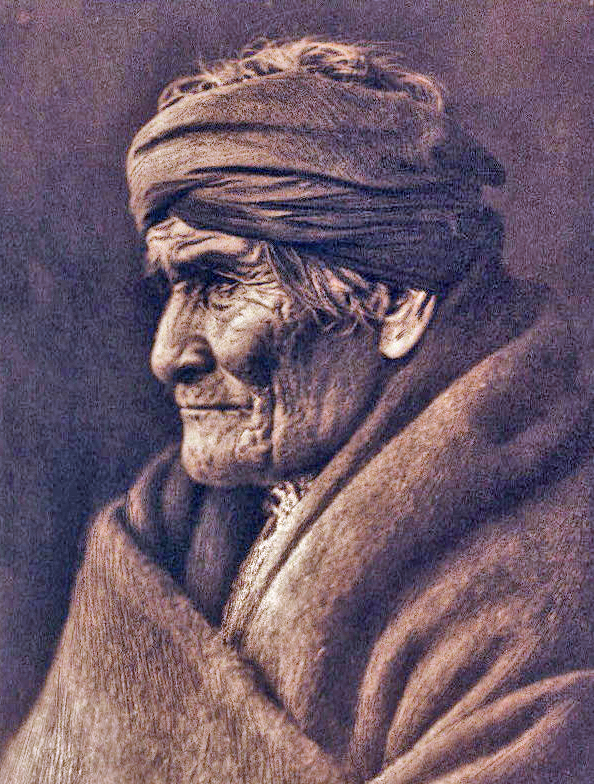
\includegraphics[width=.5\textwidth]{Geronimo.jpg}
\end{center}
\caption{In case you were wondering who Geronimo was.}
\end{figure}

\subsection{List comprehensions}

Python offers a way to combine loops, functions and logical tests in a 
single line of code. Type the following in a script file called {\tt 
oaks.py}:

\lstinputlisting{Practicals/Code/oaks.py}

Don't go mad with list comprehensions --- code readability is more 
important than squeezing lots into a single line! 

\section{Practicals}
As always, test, add, commit and push all your new code and data to 
your git repository. 

\begin{enumerate}

	\item Modify {\tt cfexercises.py} to make it a ``module'' like {\tt 
	control\_flow.py}). That is, all the {\tt fooXX} functions should 
	take arguments from the user (like the functions inside {\tt 
	control\_flow.py}. Also, add some test arguments to show that they 
	work (again, like {\tt control\_flow.py}) --- for example, 
	"foo5(10)". Thus, running {\tt cfexercises.py} should now also output 
	evaluations of all the {\tt fooXX} modules along with a bunch of 
	hellos.

	\item Open and complete the tasks in {\tt lc1.py}, 
	{\tt lc2.py}, {\tt dictionary.py}, {\tt tuple.py} (you can tackle 
	them in any order) 

\end{enumerate}

\section{Functions, Modules, and code compartmentalization}
 
 Ideally you should aim to compartmentalize your code into a bunch of 
 functions, typically written in a single {\tt .py} file: this are  
 Python ``modules'', which you were introduced to previously. Why bother 
 with modules? Because:

\begin{compactitem}
 
	\item Keeping code compartmentalized  is good for debugging, unit
  testing, and profiling (coming up later)
	\item Makes code more compact by minimizing redundancies (write
  repeatedly used code segments as a module)
	\item Allows you to import and use useful functions that you yourself
wrote, just like you would from standard python packages (coming up)
      \end{compactitem}

\subsection{Importing Modules}

There are different ways to {\bf import} a module:
\begin{compactitem}
  \item {\tt import my\_module}, then functions in the module can be called
as \\ {\tt my\_module.one\_of\_my\_functions()}.
  \item {\tt from my\_module import my\_function} imports only the
function {\tt my\_function} in the module {\tt my\_module}. It can then be
called as if it were part of the main file: {\tt my\_function()}.
  \item {\tt import my\_module as mm} imports the module
    {\tt my\_module} and calls it {\tt mm}. Convenient when the name of
the module is very long. The functions in the module can be called as
    {\tt mm.one\_of\_my\_functions()}.
  \item {\tt from my\_module import *}. Avoid doing this! \\ 
  {\it Why?} -- to avoid name conflicts!

  \item You can also access variables written into modules: {\tt import
my\_module}, then \\ {\tt my\_module.one\_of\_my\_variables}
\end{compactitem}

\section{Python packages}

A Python package is simply a directory of Python modules (quite like an 
{\tt R} package). Many packages, such as the following that I find 
particularly useful, are always available as standard libraries (just 
require {\tt import} from within python or ipython):

\begin{compactitem}
	\item {\tt io}: file input-output with {\tt *.csv}, {\tt *.txt}, etc.
	\item {\tt subprocess}: to run other programs, including multiple ones
at the same time, including operating system-dependent functionality 
	\item {\tt sqlite3}: for manipulating and querying {\tt sqlite}
databases
	\item {\tt math}: for mathematical functions
\end{compactitem}

Scores of other packages are accessible by explicitly installing them 
using \\{\tt sudo apt-get install python-packagename} (as you did 
previously) or by using {\tt pip}. Some particularly mentionable ones are:

\begin{compactitem}
		\item {\tt sciPy} (\url{http://scipy.org}) contains a wide array of numerical 
		tools  for scientific computing, including {\tt NumPy} for efficient data crunching
		\item {\tt matplotlib}: for plotting (very matlab-like, requires 
	 {\tt scipy}) (all packaged in {\tt pylab})
		\item {\tt pandas} provides a powerful set of methods to 
		manipulating data, and comes with a DataFrame object similar to the
		{\tt R} data frame.
		\item {\tt scikit-learn} \url{http://scikit-learn.org/} for applying 
		different machine learning algorithms to data
		\item {\tt ipython} an enhanced python terminal (which we are 
		currently using!) 
		\item {\tt jupyter} an interactive notebook environment for 
		exploratory data analysis, visulaization, and creation of interactive 
	 documents that can be shared. This course is in the process of being written entirely in Jupyter notebooks.
	 \item {\tt scrapy}: for writing web spiders that crawl web sites and 
	 extract data from them
	 \item {\tt beautifulsoup}: for parsing HTML and XML (can do what 
	 {\tt scrapy} does)
	 \item {\tt biopython}: for bioinformatics
\end{compactitem}
Of course, you have already installed some of these ({\tt scipy}, {\tt 
matplotlib}). 

For those of you interested in bioinformatics, the {\tt biopython} 
package will be particularly useful. We will not cover bioinformatics 
in any depth within the python weeks, but you may want to try 
to use Python for bioinformatics in other weeks, especially the 
Genomics weeks, and perhaps use it for your own research projects. I suggest that if bioinformatics is your thing, check out 
{\tt biopython} --- in particular the worked examples at 
\url{http://biopython.org/DIST/docs/tutorial/Tutorial.html}.


\section{Practicals}
As always, test, add, commit and push all your new code and data to 
your git repository. 

\subsubsection{Align DNA sequences}

Align two DNA sequences such that they are as similar as possible. 

The idea is to start with the longest string and try to position the 
shorter string in all possible positions. For each position, count a 
``score'' : number of bases matched perfectly over the number of bases 
attempted. Your tasks:

 \begin{enumerate} \itemsep3pt
 
		\item Open and run {\tt Practicals/Code/align\_seqs.py} --- make 
		sure you understand what each line is doing to do this)

		Now convert {\tt align\_seqs.py} to a Python function that 
		takes the DNA sequences as an input from a single external file and 
		saves the best alignment along with its corresponding score in a 
		single text file (your choice of format and file type) to an 
		appropriate location. No external should be needed; that is, you 
		should still only need to use {\tt python align\_seq.py} to run it. 
		
		For example, the input file can be a single {\tt .csv} file 
		with the two example sequences given at the top of the original 
		script.

		{\it Don't forget to add docstrings where necessary/appropriate.} 

		\item Extra Credit -- align all the {\tt .fasta} sequences from 
		Week 1; call the new script \\ {\tt align\_seqs\_fasta.py}. Unlike 
		align\_seqs.py, this script should take {\it any} two fasta sequences (in 
		separate files) to be aligned as input. So this script would 
		typically run by using explicit inputs, by calling something like {\tt python 
		align\_seqs\_fasta.py seq1.csv seq2.csv}. However, it should 
		still run if no inputs were given, using two fasta sequences  
		from {\tt Data} as defaults.

  \end{enumerate}

\section{Errors in your {\tt python} code}

What do you want from your code? Rank the following by importance:
  \begin{enumerate}
    \item it is very fast
    \item it gives me the right answer
    % \item it is possible to test it
    % \item it has lots of tests
    \item it is easy to read
    \item it uses lots of 'clever' programming techniques
    \item it uses cool features of the language
  \end{enumerate}

Then, think about this: 

  \begin{compactitem}
     \item If you are {\it very lucky}, your program will crash when you run it
     \item If you are {\it lucky}, you will get an answer that is obviously wrong
     \item If you are {\it unlucky}, you won't notice until after publication
     \item If you are {\it very unlucky}, someone else will notice it after 
publication
  \end{compactitem}
  
Ultimately, most of your time could well be spent error-checking and 
fixing them ``debugging'', not writing code. You can debug when errors 
appear, but why not just nip as many as you can in the bud? For this, 
you would use unit testing.

\subsection{Unit testing}

Unit testing prevents the most common mistakes and helps write reliable 
code. Indeed, there are many reasons for testing:
\begin{compactitem}
	\item Can you prove (to yourself) that your code does what you think it does?
	\item Did you think about the things that might go wrong?
	\item Can you prove to other people that your code works?
	\item Does it still all work if you fix a bug?
	\item Does it still all work if you add a feature?
	\item Does it work with that new dataset?
	\item Does it work on the latest version of the language (e.g., 
	Python 3.x vs.\ 2.7.x)?
	\item Does it work on Mac? on Linux? on Windows?
	\item Does it work on 64 bit {\it and} 32 bit?
	\item Does it work on an old version of a Mac?
	\item Does it work on Harvey, or Imperial's Linux cluster?
\end{compactitem}

The idea is to write \textit{independent} tests for the {\it smallest 
units} of code. Why the smallest units? --- to be able to retain the 
tests upon code modification. 

\subsubsection{Unit testing with {\tt doctest}}

Let's try {\tt doctest}, the simplest  testing tool in python: 
simpletests for each function are  embedded in the docstring. Copy the 
file {\tt control\_flow.py} into the file {\tt test\_control\_flow.py} 
and edit the original function so:

\lstinputlisting{Practicals/Code/test_control_flow.py}

Now type {\tt  run test\_control\_flow.py -v} :
  
\begin{lstlisting}
In []: run  test_control_flow.py -v
Trying:
    even_or_odd(10)
Expecting:
    '10 is Even!'
ok
Trying:
    even_or_odd(5)
Expecting:
    '5 is Odd!'
ok
Trying:
    even_or_odd(3.2)
Expecting:
    '3 is Odd!'
ok
Trying:
    even_or_odd(-2)
Expecting:
    '-2 is Even!'
ok
1 items had no tests:
    __main__
1 items passed all tests:
   4 tests in __main__.even_or_odd
4 tests in 2 items.
4 passed and 0 failed.
Test passed.
    \end{lstlisting}

You can also run doctest ``on the fly'', without writing  {\tt 
doctest.testmod()} in the code by typing in a terminal: {\tt python -m 
doctest -v your\_function\_to\_test.py}

\begin{tipbox}
{\it Other unit testing approaches}
	
For more complex testing, see documentation of {\tt doctest} at 
\url{https://docs.python.org/2/library/doctest.html} , the package {\tt 
nose} and the package {\tt unittest}

Please start testing as early as possible, but don't try to test 
everything either! Remember, it is easier to test if code is 
compartmentalized into functions. 
\end{tipbox}
  
\subsection{Debugging}

OK, so you unit-tested, let's go look at life through beer-goggles... 
BUT NO! YOU WILL VERY LIKELY RUN INTO BUGS!

Bugs happen, inevitably, in life and programming. You need to find and 
debug them. Banish all thoughts of littering your code with {\tt print} 
statements to find bugs. 

Enter the debugger. The command {\tt pdb} turns on the python debugger. 
Type the following in a file and save as {\tt debugme.py} in your {\tt 
Code} directory: 

\lstinputlisting{Practicals/Code/debugme.py}

Now run it:
 
   \begin{lstlisting}
In []: %run debugme.py
[lots of text]
createabug(x)
      2     y = x**4
      3     z = 0.
----> 4     y = y/z
      5     return y
      6 

ZeroDivisionError: float division by zero
  \end{lstlisting}

OK, so let's {\tt \%pdb} it
 
\begin{lstlisting}
In []: %pdb
Automatic pdb calling has been turned ON

In []: run debugme.py
[lots of text]
ZeroDivisionError: float division by zero
> createabug()
      3     z = 0.
----> 4     y = y/z
      5     return y

ipdb> 
\end{lstlisting}

Now we're in the debugger shell, and can use the following commands to 
naviagate and test the code line by line or block by block:

\begin{tipbox}
	In ``normal'' python, you would use {\tt pdb} instead of {\tt ipdb}.
\end{tipbox}

\begin{tabular}{p{1.5cm} p{11cm}} 
	{\tt n} 		& move to the next line\\
	{\tt ENTER} & repeat the previous command\\
	{\tt s} 		& ``step'' into function or procedure (i.e., continue
	  the debugging inside the function, as opposed to simply run it)\\
	{\tt p x} 	& print variable x\\
	{\tt pp locals()} 	& pretty print all variables and objects in current 
	workspace scope\\
	{\tt c} 		& continue until next break-point\\
	{\tt q} 		& quit\\
	{\tt l} 		& print the code surrounding the current position (you can
	specify how many)\\
	{\tt r} 		& continue until the end of the function\\
\end{tabular}\\


So let's continue our debugging:
  
\begin{lstlisting}
ipdb> p x
25
ipdb> p y
390625
ipdb> p z
0.0
ipdb> p y/z
*** ZeroDivisionError: ZeroDivisionError
('float division by zero',)
ipdb> l
      1 def createabug(x):
      2     y = x**4
      3     z = 0.
----> 4     y = y/z
      5     return y
      6 
      7 createabug(25)

ipdb> q

In []: %pdb
Automatic pdb calling has been turned OFF
  \end{lstlisting}

\begin{tipbox}
	Once in the debugger, use {\tt pp locals()} and/or {\tt pp globals()} to 
	see all local or global objects (including variables and functions) 
	available at the point where the debugger stopped in the 
	script. {\tt pp} stands for ``pretty print''. 
\end{tipbox}

\subsection{Paranoid programming: debugging with breakpoints}

You may want to pause the program run and inspect a given line or block 
of code ({\it why?} --- impromptu unit-testing is one reason). To do 
so, simply put this snippet of code where you want to pause and start a 
debugging session and then run the program again:
  
\begin{lstlisting}
import ipdb; ipdb.set_trace()
\end{lstlisting}

Or, you can use {\tt import pdb; pdb.set\_trace()}

Alternatively, running the code with the flag {\tt \%run -d} starts a 
debugging session from the first line of your code (you can also 
specify the line to stop at). If you are serious about programming, 
please start using a debugger (R, Python, whatever...)!

\section{Practicals}
As always, test, add, commit and push all your new code and data to 
your git repository. 

\subsubsection{Missing oaks problem}

\begin{enumerate} \itemsep8pt
	\item Open and run the code {\tt test\_oaks.py} --- there's a bug, 
	for no oaks are being found! (where's {\tt TestOaksData.csv}?)

  \item Fix the bug (hint: {\tt import ipdb; ipdb.set\_trace()})

	\item Now, write doctests to make sure that, bug or no bug, your {\tt 
	is\_an\_oak} function is working as expected (hint: {\tt $>>>$ 
	is\_an\_oak('Fagus sylvatica')} should return {\tt False})

	\item If you wrote good doctests, you will note that you found 
	another error that you might not have come across just by debugging
	(hint: what happens if you try the doctest with 'Quercuss' instead of
	'Quercus'?). How would you fix the new error you found using the 
	doctest? 

\end{enumerate}

\section{Practicals wrap-up}

  \begin{enumerate}

	\item Review and make sure you can run all the commands, code 
	fragments, and scripts we have till now and get the expected outputs 
	--- all scripts should work on any other linux laptop.

	\item Run {\tt boilerplate.py} and {\tt control\_flow.py} from 
	the bash terminal instead of from within the ipython shell (try 
	both python and ipython from the bash)
	
	\item Include an appropriate docstring (if one is missing) at the 
	beginning of {\it each} of each of the python script / module files 
	you have written, as well as at the start of every function (or 
	sub-module) in a module.

	\item Also annotate your code lines as much and as often as necessary 
	using \#.
	
	\item Keep all code files organized in {\tt 
	CMEECourseWork/Week2/Code}
	 
   \end{enumerate}

\begin{center}
	\it {\tt git add}, {\tt commit} and {\tt push} all your code and data 
	to your git repository by next Wednesday 5 PM.
\end{center}
   
\section{Readings and Resources}

\begin{compactitem} \itemsep10pt
	\item Code like a Pythonista: Idiomatic {\tt python} (Google it)
	\item Also good: the Google {\tt python} Style Guide
	\item Browse the python tutorial: \url{https://docs.python.org/3/tutorial/}
	\item For functions and modules:\\
	\url{https://learnpythonthehardway.org/book/ex40.html}
	\item For IPython:\\
		\url{http://ipython.org/ipython-doc/stable/interactive/tips.html}
  \item Cookbooks can be very useful: 
  \url{https://github.com/ipython/ipython/wiki}
	\item Look up \url{https://docs.python.org/2/library/index.html} -- Read 
	about the packages you think will be important to you
	\item Some of you might find the python package {\tt biopython} 
	particularly useful --- check out \url{http://biopython.org/}, and especially, the cookbook
\end{compactitem}
In general, scores of good module/package-specific cookbooks are out there --- google "cookbook" along with the name of the package you are interested in (e.g., ``scipy cookbook'').

\chapter{Advanced Biological Computing in Python}
\label{chap:pythonII}

\epigraph{...some things in life are bad. They can really make you mad. 
Other things just make you swear and curse. When you're chewing on 
life's gristle, don't grumble; give a whistle, and this'll help things 
turn out for the  best. And... always look on the bright side of 
life...}{\textit{---Guess who?}}

In this chapter, we will cover a some topics in Python that will 
round-off your python training:
\begin{itemize}
	\item Numerical computing in python 
	\item ``Reading'' text data using regular expressions in python
	\item Databases, and using python to build and manage them
	\item Using python to build workflows
	% \item Interactive analysis and visualization of mathematical models as well as data using jupyter notebooks
\end{itemize}  
{\it The last topic will be necessary for your Miniproject, which will 
involve building a reproducible computational workflow.  }

\section{Numerical computing in {\tt python}}

The python package {\tt scipy} can help you do serious number crunching 
including,
	\begin{compactitem}
		\item Linear algebra (matrix and vector operations)
		\item Numerical integration (Solving ODEs)
		\item Fourier transforms
		\item Interpolation
		\item Calculating special functions (incomplete Gamma, Bessel, etc.)
		\item Generation of random numbers
		\item Using statistical functions and transformations
	\end{compactitem}
	
In the following, we will use the {\tt array} data structure in {\tt 
scipy} for data manipulations and calculations. Scipy arrays are 
objects, and are similar in some respects to python lists, but are more 
naturally multidimensional, homogeneous in type (the default is float), 
and allow efficient (fast) manipulations. Thus scipy arrays are 
analogous to the R {\tt matrix} data object/structure. 

\begin{tipbox}
	The same array objects are accessible within the {\tt numpy} package, which 
is a subset of {\tt scipy}.
\end{tipbox}

So let's try {\tt scipy}:
 \begin{lstlisting}
In []: import scipy

In []: a = scipy.array(range(5)) # a one-dimensional array

In []: a
Out[]: array([0, 1, 2, 3, 4])

In []: type(a)
Out[]: numpy.ndarray

In []: type(a[0])
Out []: numpy.int64
\end{lstlisting}

So all elements in {\tt a} are of type {\tt int} because that is what 
{\tt range()} returns (try {\tt ?range}).

\begin{figure}[H] \centering
    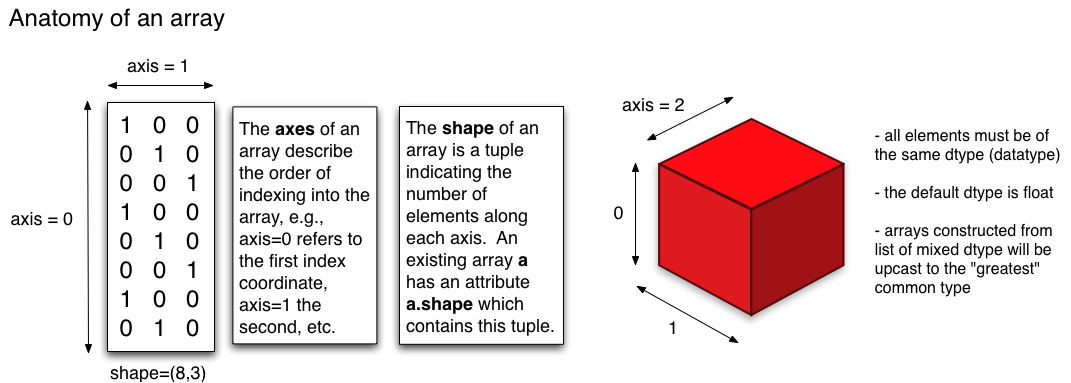
\includegraphics[width=1\textwidth]{numpyarray.png}
	\caption{A graphical depiction of numpy/scipy arrays, which can have 
	multiple dimensions (even greater than 3). From 
	\url{http://pages.physics.cornell.edu/~myers/teaching/ComputationalMethods/python/arrays.html}}
\end{figure}

You can also specify the data type of the array:

\begin{lstlisting}
In []: a = scipy.array(range(5), float)

In []: a
Out[]: array([ 0.,  1.,  2.,  3.,  4.])

In []: a.dtype # Check type 
Out[]: dtype('float64')
\end{lstlisting}

You can also get a 1-D arrays as follows: 
\begin{lstlisting}
In []: x = scipy.arange(5)

In []: x
Out[8]: array([0, 1, 2, 3, 4])

In [9]: x = scipy.arange(5.) #directly specify float using decimal

In [10]: x
Out[10]: array([ 0.,  1.,  2.,  3.,  4.])
\end{lstlisting}

As with other Python variables (e.g., created as a list or a 
dictionary), you can apply methods to variables created as scipy 
arrays. For example, TAB after {\tt x.} to see methods you can apply to 
{\tt x}:
\begin{lstlisting}
In [11]: x. 
x.T             x.conj          x.fill          
x.nbytes        x.round         x.take
x.all           x.conjugate     x.flags         
x.ndim          x.searchsorted  x.tofile
x.any           x.copy          x.flat          
x.newbyteorder  x.setfield      x.tolist
x.argmax        x.ctypes        x.flatten       
x.nonzero       x.setflags      x.tostring
x.argmin        x.cumprod       x.getfield      
x.prod          x.shape         x.trace
x.argsort       x.cumsum        x.imag         
x.ptp           x.size          x.transpose
x.astype        x.data          x.item          
x.put           x.sort          x.var
x.base          x.diagonal      x.itemset       
x.ravel         x.squeeze       x.view
x.byteswap      x.dot           x.itemsize      
x.real          x.std           
x.choose        x.dtype         x.max           
x.repeat        x.strides       
x.clip          x.dump          x.mean          
x.reshape       x.sum           
x.compress      x.dumps         x.min           
x.resize        x.swapaxes      

In [12]: x.shape
Out[12]: (5,)
\end{lstlisting}

\begin{tipbox}
	Remember, you can type {\tt :?x.methodname} to get info on a particular method. For 
example, try {\tt ?x.shape}.
\end{tipbox}

You can also convert to and from Python lists:

\begin{lstlisting}
In []: b = scipy.array([i for i in range(100) if i%2==1]) #odd numbers 
between 1 and 100

In []: c = b.tolist() #convert back to list
 \end{lstlisting}

To make a  matrix, you need a 2-D scipy array:
\begin{lstlisting}
In [14]: mat = scipy.array([[0, 1], [2, 3]])

In []: mat.shape
Out[]: (2, 2)
\end{lstlisting}

\subsection{Indexing and accessing arrays}

As with other Python data objects such as lists, scipy array elements 
can be accessed using square brackets ([]) with the [row,column] 
reference. Indexing of scipy arrays works 
like that for other data strauctures, with index values starting at 0. 
So, you can obtain all the elements of a particular row as:
\begin{lstlisting}
In []: mat[1] # accessing whole 2nd row, remember indexing starts at 
0
Out[]: array([2, 3])

In [57]: mat[:,1] #accessing whole second column  
Out[57]: array([1, 3])
\end{lstlisting}

And accessing particular elements: 
\begin{lstlisting}
In []: mat[0,0] # 1st row, 1st column element
Out[]: 0
In []: mat[1,0] # 2nd row, 1st column element
Out[]: 2
\end{lstlisting}
Note that (like all other programming languages) row index always comes 
before column index. That is, {\tt mat[1]} is always going to mean 
``whole second row'', and {\tt mat[1,1]} means 1st row and 1st column 
element. Therefore, to access the whole second column, you need:
\begin{lstlisting}
In []: mat[:,0] #accessing whole first column  
Out[]: array([0, 2])
\end{lstlisting}

\begin{tipbox}
Python indexing also accepts negative values for going back to the 
start from the end of an array:
\begin{lstlisting}
In []: mat[0,1]
Out[]: 1

In []: mat[0,-1] #interesting!
Out[]: 1

In []: mat[0,-2] #very interesting, perhaps useless!
Out[]: 0
\end{lstlisting}
\end{tipbox}

\subsection{Manipulating arrays}
Manipulating {\tt scipy} arrays is pretty straightforward.
 
 
\begin{tipbox}
A NumPy array is basically described by metadata (number of dimensions, shape, data type, and so on) and the actual data. The data is stored in a homogeneous and contiguous block of memory, at a particular address in system memory (Random Access Memory, or RAM). This block of memory is called the data buffer. This is the main difference with a pure Python structure, like a list, where the items are scattered across the system memory. This aspect is the critical feature that makes NumPy arrays so efficient.
\end{tipbox}

\subsubsection{Replacing, adding or deleting elements} 

Let's look at how you can replace, add, or delete an array element (a 
single entry, or whole row(s) or whole column(s)):

\begin{lstlisting}
In []: mat[0,0] = -1 #replace a single element

In []: mat
Out[]: 
array([[-1,  1],
       [ 2,  3]])
       
In []: mat[:,0] = [12,12] #replace whole column

In []: mat
Out[]: 
array([[12,  1],
       [12,  3]])

In []: scipy.append(mat, [[12,12]], axis = 0) #append row, note axis 
specification
Out[]: 
array([[12,  1],
       [12,  3],
       [12, 12]])

In []: scipy.append(mat, [[12],[12]], axis = 1) #append column
Out[]: 
array([[12,  1, 12],
       [12,  3, 12]])

In []: newRow = [[12,12]] #create existing row

In []: mat = scipy.append(mat, newRow, axis = 0) #append that existing row
Out[]: 
array([[12,  1],
       [12,  3],
       [12, 12]])

In []: scipy.delete(mat, 2, 0) #Delete 3rd row
Out[]: 
array([[12,  1],
       [12,  3]])
\end{lstlisting}

And concatenation:

\begin{lstlisting}
In []: mat = scipy.array([[0, 1], [2, 3]])

In []: mat0 = scipy.array([[0, 10], [-1, 3]])

In []: scipy.concatenate((mat, mat0), axis = 0)
Out[]: 
array([[ 0,  1],
       [ 2,  3],
       [ 0, 10],
       [-1,  3]])
\end{lstlisting}
 
\subsubsection{Flattening or reshaping arrays} 
You can also ``flatten'' or ``melt'' arrays, that is, change array 
dimensions (e.g., from a matrix to a vector):
\begin{lstlisting}
In []: mat.ravel()
Out[]: array([0, 1, 2, 3]) # NOTE: ravel is row-priority

In []: mat.reshape((4,1)) # this is different from ravel - check ?scipy.reshape
Out[66]: 
array([[0],
       [1],
       [2],
       [3]])

In []: mat.reshape((1,4)) # NOTE: reshaping is also row-priority
Out[]: array([[0, 1, 2, 3]])

In []: mat.reshape((3, 1)) # But total elements must remain the same!
---------------------------------------------------------------------------
ValueError                                Traceback (most recent call last)
<ipython-input-81-ba16cb0744eb> in <module>()
----> 1 mat.reshape((3, 1))

ValueError: total size of new array must be unchanged
\end{lstlisting}
This is a bit different than how {\tt R} behaves (coming up in Chapters 
(\ref{chap:RI}--\ref{chap:R_II} )), where you won't get an error ({\tt 
R} ``recycles'' data), which is more dangerous!

\subsection{Pre-allocating arrays}
As in other computer languages, it is usually more efficient to 
preallocate a array rather than append / insert / concatenate addtional 
elelents, rows, or columns. For example, if you know the size of your 
matrix or array, you can inititalize it with ones or zeros:

\begin{lstlisting}
In []: scipy.ones((4,2)) #(4,2) are the (row,col) array dimensions
Out[]: 
array([[ 1.,  1.],
       [ 1.,  1.],
       [ 1.,  1.],
       [ 1.,  1.]])

In []: scipy.zeros((4,2)) # or zeros
Out[]: 
array([[ 0.,  0.],
       [ 0.,  0.],
       [ 0.,  0.],
       [ 0.,  0.]])

In []: m = scipy.identity(4) #create an identity matrix

In []: m
Out[]: 
array([[ 1.,  0.,  0.,  0.],
       [ 0.,  1.,  0.,  0.],
       [ 0.,  0.,  1.,  0.],
       [ 0.,  0.,  0.,  1.]])

In []: m.fill(16) #fill the matrix with 16

In []: m
Out[26]: 
array([[ 16.,  16.,  16.,  16.],
       [ 16.,  16.,  16.,  16.],
       [ 16.,  16.,  16.,  16.],
       [ 16.,  16.,  16.,  16.]])
\end{lstlisting}

\subsection{{\tt scipy} matrices}

Scipy also has a {\tt matrix} data structure class. Scipy matrices are 
strictly 2-Dimensional, while scipy arrays are N-Dimensional. Matrix 
objects are a subclass of scipy arrays, so they inherit all the 
attributes and methods of scipy arrays (also called ``ndarrays'').

\begin{tipbox}
The main advantage of scipy matrices is that they provide a convenient 
notation for matrix multiplication: if a and b are matrices, then a*b 
is their matrix product.
\end{tipbox}

\subsubsection{Matrix-vector operations}
Now let's perform some common matrix-vector operations on arrays (you 
also try the same using matrices instead of arrays):
  
\begin{lstlisting}
In []: mm = scipy.arange(16)

In []: mm = mm.reshape(4,4) #Convert to matrix

In []: mm.transpose()
Out[]: 
array([[ 0,  4,  8, 12],
       [ 1,  5,  9, 13],
       [ 2,  6, 10, 14],
       [ 3,  7, 11, 15]])

In [6]: mm + mm.transpose()
Out[6]: 
array([[ 0,  5, 10, 15],
       [ 5, 10, 15, 20],
       [10, 15, 20, 25],
       [15, 20, 25, 30]])

In [7]: mm - mm.transpose()
Out[7]: 
array([[ 0, -3, -6, -9],
       [ 3,  0, -3, -6],
       [ 6,  3,  0, -3],
       [ 9,  6,  3,  0]])

In [8]: mm * mm.transpose()
## Elementwise!

Out[8]: 
array([[  0,   4,  16,  36],
       [  4,  25,  54,  91],
       [ 16,  54, 100, 154],
       [ 36,  91, 154, 225]])

In [9]: mm / mm.transpose()
Warning: divide by zero encountered in divide

# Note the integer division
Out[9]: 
array([[0, 0, 0, 0],
       [4, 1, 0, 0],
       [4, 1, 1, 0],
       [4, 1, 1, 1]])

In [10]: mm * scipy.pi
Out[10]: 
array([[  0.      ,   3.14159,   6.28318531,   9.42477796],
       [ 12.566370,  15.70796,  18.84955592,  21.99114858],
       [ 25.132741,  28.27433,  31.41592654,  34.55751919],
       [ 37.699111,  40.84070,  43.98229715,  47.1238898 ]])

In [11]: mm.dot(mm) # MATRIX MULTIPLICATION
Out[11]: 
array([[ 56,  62,  68,  74],
       [152, 174, 196, 218],
       [248, 286, 324, 362],
       [344, 398, 452, 506]])
\end{lstlisting}

We can do a lot more (but won't!) by importing the {\tt linalg} 
sub-package: {\tt scipy.linalg}. 

\subsection{Two useful {\tt scipy} sub-packages}

Two particularly useful {\tt scipy} sub-packages are {\tt 
scipy.integrate} (what will I need this for?) and {\tt scipy.stats}. 
Why not use {\tt R} for this? --- because often you might just want to 
calculate some summary stats of your simulation results within Python.  

\subsubsection{{\tt scipy.stats}}
Let's take a quick spin in {\tt scipy.stats}.

\begin{lstlisting}
In [18]: import scipy.stats

In [19]: scipy.stats.
scipy.stats.arcsine               scipy.stats.lognorm
scipy.stats.bernoulli             scipy.stats.mannwhitneyu
scipy.stats.beta                  scipy.stats.maxwell
scipy.stats.binom                 scipy.stats.moment
scipy.stats.chi2                  scipy.stats.nanstd
scipy.stats.chisqprob             scipy.stats.nbinom
scipy.stats.circvar               scipy.stats.norm
scipy.stats.expon                 scipy.stats.powerlaw
scipy.stats.gompertz              scipy.stats.t
scipy.stats.kruskal               scipy.stats.uniform

In [19]: scipy.stats.norm.rvs(size = 10) # 10 samples from 
N(0,1)
Out[19]: 
array([-0.951319, -1.997693,  1.518519, -0.975607,  0.8903,
       -0.171347, -0.964987, -0.192849,  1.303369,  0.6728])

In [20]: scipy.stats.norm.rvs(5, size = 10) 
# change mean to 5
Out[20]: 
array([ 6.079362,  4.736106,  3.127175,  5.620740,  5.98831,
        6.657388,  5.899766,  5.754475,  5.353463,  3.24320])

In [21]: scipy.stats.norm.rvs(5, 100, size = 10) 
# change sd to 100
Out[21]: 
array([ -57.886247,   12.620516,  104.654729,  -30.979751,
         41.775710,  -31.423377,  -31.003134,   80.537090,
          3.835486,  103.462095])

# Random integers between 0 and 10
In [23]: scipy.stats.randint.rvs(0, 10, size =7)
Out[23]: array([6, 6, 2, 0, 9, 8, 5])
\end{lstlisting}

\subsubsection{{\tt scipy.integrate} -- the Lotka-Volterra model} 
Numerical integration is the approximate computation of an integral 
using numerical techniques. You need numerical integration whenever you 
have a complicated function that cannot be integrated analytically 
using anti-derivatives. A common application is solving ordinary 
differential equations (ODEs), commonly used for modelling biological 
systems.

Let's try {\tt scipy.integrate} for solving a classical model in biology 
--- the Lotka-Volterra model for a predator-prey system. 

\begin{compactitem}[$\quad\star$]\itemsep4pt
	\item Create {\tt LV1.py} in your weekly directory and run it.
\end{compactitem}
 The 
Lotka-Volterra model is: 
\begin{equation}\label{eqn:LVMod}
\begin{aligned}
    \frac{dR}{dt} &= r R - a C R \\
    \frac{dC}{dt} &= - z C + e a C R
\end{aligned}
\end{equation}

where $C$ and $R$ are consumer (e.g., predator) and resource (e.g., 
prey) population sizes (either biomass or numbers), $r$ is the 
intrinsic growth rate of the resource population, $a$ is a "search 
rate" that determines the encounter rate between consumer and resource, 
$z$ is mortality rate and $e$ is the consumer's efficiency in converting 
resource to consumer biomass. 

{\tt LV1.py} runs (numerically solves the ODE) this model and plots the 
equilbrium. Have good look at the code, line by line, and make sure 
that you understand what's going on. A subsequent practical will 
require you to use this code to simulate modified version od the LV 
model.   

\section{The need for speed: Profiling in Python}

Donald Knuth says: {\it Premature optimization is the root of all 
evil}. Indeed, computational speed may not be your initial concern. 
Also, you should focus on developing clean, reliable, reusable code 
rather than worrying first about how fast your code runs. However, 
speed will become an issue when and if your analysis or modeling 
becomes complex enough (e.g., food web or large network simulations). 
In that case, knowing which parts of your code take the most time is 
useful -- optimizing those parts may save you lots of time. To find out 
what is slowing down your code you need to use ``profiling''. 

\subsection{Profiling}

Profiling is easy in {\tt ipython} -- simply type the 
magic command {\tt \%run -p your\_function\_name}. 

Let's write a simple illustrative program and name it {\tt 
profileme.py}:
\lstinputlisting{Practicals/Code/profileme.py}

Now {\tt \%run -p profileme.py}, and you should see something like:
  
\begin{lstlisting}
         54 function calls in 3.652 seconds

   Ordered by: internal time

   ncalls  tottime  percall  cumtime  percall filename:lineno(function)
        1    2.744    2.744    3.648    3.648 profileme.py:1(a_useless_function)
        2    0.905    0.452    0.905    0.452 {range}
        1    0.002    0.002    0.003    0.003 profileme.py:8(a_less_useless_function)
[more output]        
\end{lstlisting}
     
The function {\tt range} is taking long -- we should use {\tt xrange} 
instead. When iterating over a large number of values, {\tt xrange}, 
unlike {\tt range}, does not create all the values before iteration, 
but creates them "on demand" (ie.e., {\tt xrange} is a ``generator''). Range creates a list, so if you do {\tt range(1, 10000000)} it creates a list in memory with 10000000 elements. For example, {\tt range(1000000)}yields a 4Mb+ list. 

So let's modify the script:

\lstinputlisting{Practicals/Code/profileme2.py}

Again running the magic command {\tt \%run -p} yields:

\begin{lstlisting}
         52 function calls in 2.153 seconds

   Ordered by: internal time

   ncalls  tottime  percall  cumtime  percall filename:lineno(function)
        1    2.150    2.150    2.150    2.150 profileme2.py:1(a_useless_function)
        1    0.002    0.002    0.002    0.002 profileme2.py:8(a_less_useless_function)
        1    0.001    0.001    2.153    2.153 {execfile}
 [more output]

\end{lstlisting}
    
So we saved 1.499 s! (not enough to grab a pint, but ah well...).

\subsection{Quick profiling with {\tt timeit}}
Alternatively, if you are writing your script and want to figure out 
what the best way to do something (say a particular command or 
a loop) might be, then you can use {\tt timeit}. 

Type an run the following code in a python script called {\tt 
timeitme.py}:

\lstinputlisting{Practicals/Code/timeitme.py}

Now run it these different instances of timeit-ing by tying the {\tt \% 
timeit} command followed by the function call. Note that You can import 
all the functions using {\tt from timeitme import *}  

But remember, don't go crazy with profiling for the sake of shaving a 
couple of milliseconds, tempting as that may be!

%Insert section on speeding up code here
% This will include vectorization, local parallelization, and cython
 
%Cython:
% Make sure you have the latest version of Cython from pip. Various linux package managers are out of date.
% Rename your numeric code module's .py file to .pyx,
% Use pyximport from the main script ( http://docs.cython.org/src/userguide/source_files_and_compilation.html#pyximport ) to have it compiled at runtime without any extra build steps, and then
% Start experimenting with adding a few "cdef"s (http://docs.cython.org/src/quickstart/cythonize.html and http://docs.cython.org/src/tutorial/numpy.html)
% The static typing part is the main speedup. Cython does speed up pure python code slightly - but if you add static C types, it can eliminate it entirely and run your algorithm without creating a Python object for each int or double.

% Parallel programming
% http://scipy-cookbook.readthedocs.org/items/ParallelProgramming.html

%f2py

\section{Practicals}

As always, test, add, commit and push all your new code and data to 
your git repository. 

\subsubsection{Lotka-Volterra model problem} 

Copy and modify {\tt LV1.py} into another script called {\tt LV2.py} 
that does the following:

\begin{enumerate}
	\item Take arguments for the four LV model parameters $ r, a, z ,e$ 
	from the commandline
\begin{lstlisting}
 LV2.py arg1 arg2 ... etc
\end{lstlisting}
	\item Runs the Lotka-Volterra model with prey density dependence $r R 
	(1 - \frac{R} {K})$, which changes the coupled ODEs to,
\begin{equation}
	\begin{aligned}
	    \frac{dR}{dt} &= r R (1 - \frac{R} {K}) - a C R \\
	    \frac{dC}{dt} &= - z C + e a C R
	\end{aligned}
\end{equation}

	\item Saves the plot as {\tt .pdf} in an external results directory in your weekly directory 
	\item The chosen parameter values should show in the plot (e.g., $r = 1, a = .5 $, etc)  
You can change time length $t$ too. 
	
	\item Include a script in {\tt Code} that will run both {\tt LV1.py} 
	and {\tt LV2.py} with appropriate arguments. This script should also 
	profile the two scripts and print the results to screen for each of 
	the scripts using the {\tt \%run -p} approach. Look at and compare 
	the speed bottlenecks in {\tt LV1.py} and {\tt LV2.py}. Think about 
	how you could further speed up the scripts. 
	 
\end{enumerate}

{\it Write every subsequent extra credit script file with a new name 
such as {\tt LV3.py},{\tt LV4.py}, etc. }

{\bf Extra credit}: Choose appropriate values for the parameters such 
that both predator and prey persist with prey density dependence --- 
the final (non-zero) population values should be printed to screen. 

{\bf Extra-extra credit}: Write a discrete-time version of the LV 
model called {\tt LV3.py}. The discrete-time model is: 
\begin{equation}\label{eqn:LVDisc} 
	\begin{aligned} 
		R_{t+1} &= R_t (1 + r (1 - \frac{R_t}{K}) - a C_t)\\ 
		C_{t+1} &= C_t (1 - z + e a R_t) 
	\end{aligned} 
\end{equation}
Include this script in {\tt run\_LV.py}, and profile it as well. 

{\bf Extra-extra-extra credit}: Write a version of the discrete-time 
model (eqn \ref{eqn:LVDisc}) simulation with a random gaussian 
fluctuation in resource's growth rate at each time-step: 
\begin{equation}\label{eqn:LVFluc1}
	\begin{aligned}
		R_{t+1} &= R_t (1 + (r + \epsilon) (1 - \frac{R_t}{K})- a C_t)\\
		C_{t+1} &= C_t (1 - z + e a R_t)
	\end{aligned}
\end{equation}
where $\epsilon$ is a random fluctuation drawn from a gaussian 
distribution (use {\tt scipy.stats}). Include this script in {\tt 
run\_LV.py}, and profile it as well. 

You can also add fluctuations to both populations simultaneously this way: 
\begin{equation}\label{eqn:LVFluc2}
	\begin{aligned}
		R_{t+1} &= R_t (1 + \epsilon + r +  (1 - \frac{R_t}{K}) - a C_t)\\
		C_{t+1} &= C_t (1 - z + \epsilon + e a R_t)
	\end{aligned} 
\end{equation}

\section{Networks in {\tt python} (and R)}

ALL biological systems have a network representation, consisting of 
nodes for the biological entities of interest, and edges or links for 
the relationships between them. Here are some examples:

\begin{compactitem}
	\item Metabolic networks
	\item Gene regulatory networks
	\item Individual-Individual (e.g., social networks)
	\item Food webs
	\item Pollination networks
\end{compactitem} 
{\it Can you think of a few more examples from biology?}

You can easily simulate, analyze, and visualize biological networks in 
both {\tt python} and {\tt R} using some nifty packages. A full network 
anaalysis tutorial is out of the scope of our Python module's 
objectives, but let's try a simple visualization using the {\tt 
networkx} python package. 

For this you need to first install the package:

\begin{lstlisting}
$ sudo apt-get install python-networkx	
\end{lstlisting}
 
Now type the code file {\tt DrawFW.py} and run it:

\lstinputlisting{Practicals/Code/DrawFW.py}

Look thorugh the code carefully (line-by-line) as there are some new 
python objects introduced by {\tt networkx} for storing node and edge data.

\section{Practicals}

You can also do nice network visualizations in R. Here you will convert 
a network visualization script written in {\tt R} using the {\tt 
igraph} package to a python script that does the same thing.  

First copy the script file called {\tt Nets.R} and the data files it 
calls and run it. This script visualizes the QMEE CDT collaboration 
network (see \url{http://www.imperial.ac.uk/qmee-cdt/}), coloring the 
the nodes by the type of node (organization type: 
``University'',``Hosting Partner'', ``Non-hosting Partner''). 

Now, convert this script to a {\tt python} script that does the same 
thing, including writing to an {\tt *.svg} file using the same QMEE CDT 
link and node data. You can use {\tt networkx} or some other python 
network visualization package.

\section{Regular expressions in {\tt python}}

Let's shift gears now, and look at a very important skill that you 
should learn, or at least be aware of --- {\it Regular expressions}. 
Regular expressions (regex) are a tool to find patterns in strings, 
such as:
\begin{compactitem}
	\item Finding DNA motifs in sequence data
	\item Navigating through files in a directory
	\item Parsing text files
	\item Extracting information from html and xml files
\end{compactitem}
Thus, if you are interested in data mining, need to clean or process 
data in any other way, or convert a bunch of information into usable 
data, knowing regex is necessary. 
\begin{figure}[H] \centering
	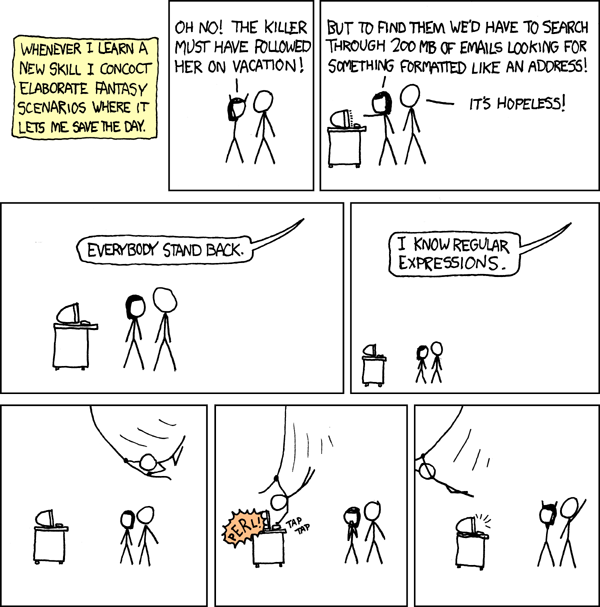
\includegraphics[width = .6\textwidth]{regex.png}\\
	\url{www.xkcd.com/208/}
\end{figure}

Regex packages are available for most programming languages ({\tt grep} 
in UNIX / Linux, where regex first became popular).

\subsection{Metacharacters vs. regular characters}
A regex may consist of a combination of ``metacharacters'' (modifiers) 
and ``regular'' or literal characters. There are 14 metacharacters: {\tt 
[ ] \{ \} ( ) \textbackslash~ \^{} \$ . $\vert$ ? * + }     
These metacharacters do special things, for example:
\begin{compactitem}
	\item {\tt [12]} means match target to {\tt 1} and if that does not match
then match target to {\tt 2}
	\item {\tt [0-9]} means match to any character in range {\tt 0} to 
	{\tt 9}
	\item {\tt [\^{}Ff]} means anything except upper or lower case {\tt 
	f} and 
	{\tt [\^{}a-z]} means everything except lower case {\tt a} to {\tt z}
\end{compactitem}
Everything else is interpreted literally (e.g., {\tt a} is matched by 
entering {\tt a} in the regex). 

{\tt [ } and {\tt ] }, specify a character ``class'' --- the set of 
characters that you wish to match. Metacharacters are not active inside 
classes. For example, {\tt [a-z\$]} will match any of the characters 
{\tt a} to {\tt z}, but also {\tt \$}, because inside a character class 
it loses its special metacharacter status.

\subsection {regex elements}

A useful (not exhaustive) list of regex elements is: 

\begin{tabular}{p{2cm} p{10cm}} 
 {\tt a} & match the character {\tt a}\\
 {\tt 3} & match the number {\tt 3}\\
 {\tt $\backslash$n} & match a newline\\
 {\tt $\backslash$t} & match a tab\\
 {\tt $\backslash$s} & match a whitespace\\
 {\tt .} & match any character except line break (newline)\\
 {\tt $\backslash$w} & match any alphanumeric character (including
underscore)\\
 {\tt $\backslash$W} & match any character not covered by {\tt 
 $\backslash$w} (i.e., match any non-alphanumeric character excluding 
 underscore)\\
 {\tt $\backslash$d} & match a numeric character\\
 {\tt $\backslash$D} & match any character not covered by {\tt 
 $\backslash$d} (i.e., match a non-digit)\\
 {\tt [atgc]} & match any character listed: {\tt a}, {\tt t}, {\tt g}, 
 {\tt c}\\
 {\tt at|gc} & match {\tt at} or {\tt gc}\\
 {\tt [$\hat{\,}$atgc]} & any character not listed: any character but 
 {\tt a}, {\tt t}, {\tt g}, {\tt c}\\
 {\tt ?} & match the preceding pattern element zero or one times\\
 {\tt *} & match the preceding pattern element zero or more times\\
 {\tt +} & match the preceding pattern element one or more times\\
 {\tt \{n\}} & match the preceding pattern element exactly {\tt n} times\\
 {\tt \{n,\}} & match the preceding pattern element at least {\tt n} times\\
 {\tt \{n,m\}} & match the preceding pattern element at least {\tt n}
but not more than {\tt m} times\\
 {\tt \textasciicircum} & match the beginning of a line\\
 {\tt \$} & match the end of a line\\
  \end{tabular}

\subsection {regex in {\tt python}}

Regex functions in python are in the module {\tt re} --- so we will 
{\tt import re}. The simplest {\tt python} regex function is {\tt 
re.search}, which searches the string for match to a given pattern --- 
returns a \textit{match object} if a match is found and {\tt None} if 
not. 

\begin{tipbox}
	
{\bf Always} put {\tt r} in front of your regex --- it tells python to 
read the regex in its ``raw'' (literal) form. Without raw string 
notation (r"text"), every backslash ('\textbackslash') in a regular 
expression would have to be prefixed with another one to escape it. 

From \url{https://docs.python.org/2/library/re.html}: {\it If you're 
not using a raw string to express the pattern, remember that Python 
also uses the backslash as an escape sequence in string literals; if 
the escape sequence isn't recognized by Python's parser, the backslash 
and subsequent character are included in the resulting string. However, 
if Python would recognize the resulting sequence, the backslash should 
be repeated twice. This is complicated and hard to understand, so it's 
highly recommended that you use raw strings for all but the simplest 
expressions.}
\end{tipbox}

OK, let's try some regexes (type all that follows in {\tt 
Code/regexs.py}):

\lstinputlisting{Practicals/Code/re1.py}

 To know whether a pattern was matched, we can use an {\tt if}:

\begin{lstlisting}
MyStr = 'an example'

match = re.search(r'\w*\s', MyStr)

if match:                      
    print 'found a match:', match.group() 
else:
    print 'did not find a match'    
\end{lstlisting}
  
Here are some more regexes (add all that follows to the {\tt Code/regexs.py}):

\lstinputlisting{Practicals/Code/re2.py}

\begin{figure}[H] \centering
    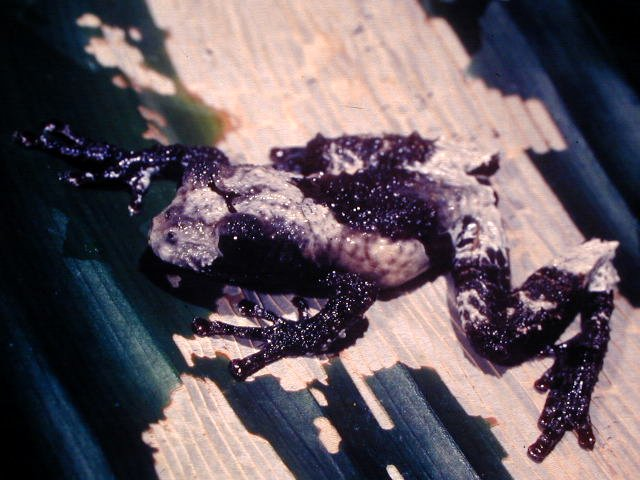
\includegraphics[width=.5\textwidth]{thelodermaasper.JPG}
\caption{In case you were wondering what {\it Theloderma asper}, the 
``bird-shit frog'', looks like. I snapped this one in North-east India ages 
ago}
\end{figure}

You can group regexes into meaningful blocks using parentheses. For 
example, let's try matching a string consisting of an academic's name, 
email address and research area or interest (no need to type this into 
any python file): 
  
\begin{lstlisting}
MyStr = 'Samraat Pawar, s.pawar@imperial.ac.uk, Systems biology and 
ecological theory'

# without groups
match = re.search(r"[\w\s]*,\s[\w\.@]*,\s[\w\s&]*",MyStr)

match.group()
'Samraat Pawar, s.pawar@imperial.ac.uk, Systems biology and ecological theory'

match.group(0)
'Samraat Pawar, s.pawar@imperial.ac.uk, Systems biology and ecological theory'

# now add groups using ( )
match = re.search(r"([\w\s]*),\s([\w\.@]*),\s([\w\s&]*)",MyStr)

match.group(0)
'Samraat Pawar, s.pawar@imperial.ac.uk, Systems biology and ecological theory'

match.group(1)
'Samraat Pawar'

match.group(2)
's.pawar@imperial.ac.uk'

match.group(3)
'Systems biology and ecological theory'
\end{lstlisting}

Have a look at {\tt re4.py} in your code repository for more on parsing 
email addresses using regexes.  

\subsection{Some RegExercises}

These exercises are not for submission as part of your coursework, but 
we will discuss them in class (in a later week).

\begin{enumerate}\itemsep16pt

	 \item Translate the following regular expressions into regular 
	 English (don't type this in {\tt regexs.py})!
  
\begin{lstlisting}
r'^abc[ab]+\s\t\d'
% 'abca \t1'

r'^\d{1,2}\/\d{1,2}\/\d{4}$'
% '11/12/2004'

r'\s*[a-zA-Z,\s]+\s*'
% ' aBz  '
\end{lstlisting}
  
\item Write a regex to match dates in format YYYYMMDD, making sure that:
     \begin{compactitem}
      \item Only seemingly valid dates match (i.e., year greater than 1900)
      \item First digit in month
 is either 0 or 1
      \item First digit in day $\leq$ 3
     \end{compactitem}
  
  \end{enumerate}
  
  %re.search(r'19\d{2}[01]\d[0-3]\d|20\d{2}[01]\d[0-3]\d', 'whatabout 19001212 ?').group()
  
  %Same, but shorter:
  % re.search(r'(19|20)\d{2}[01]\d[0-3]\d', 'whatabout 19001212?').group()

	% A more robust solution (Leanne Massie 2015-16 batch):

  % re.search(r'((19)|(20))\d{2}((0\d)|(10)|(11)|(12))([012]\d|((30)|(31)))' ,'whatabout 19001212 ?').group()
  % re.search(r'((19)|(20))\d{2}((0\d)|(10)|(11)|(12))([012]\d|((30)|(31)))' ,'whatabout 19001235 ?').group()  

\subsection{Important {\tt re} functions}

\begin{tabular}{p{5.4cm} p{9cm}} 
   
  {\tt re.compile(reg)} & Compile a regular expression. In this way
    the pattern is stored for repeated use, improving the speed.\\

	{\tt re.search(reg, text)} & Scan the string and find the first match 
	of the pattern in the string. Returns a {\tt match} object if 
	successful and {\tt None} otherwise.\\

	{\tt re.match(reg, text)} & as {\tt re.search}, but only match the 
	beginning of the string.\\

	{\tt re.split(ref, text)} & Split the text by the occurrence of the 
	pattern described by the regular expression.\\

	{\tt re.findall(ref, text)} & As {\tt re.search}, but return a list 
	of all the matches. If groups are present, return a list of groups.\\

	{\tt re.finditer(ref, text)} & As {\tt re.search}, but return an 
	iterator containing the next match.\\

	{\tt re.sub(ref, repl, text)} & Substitute each non-overlapping 
	occurrence of the match with the text in {\tt repl} (or a 
	function!).\\

\end{tabular}

\section{Practicals}
As always, test, add, commit and push all your new code and data to 
your git repository. 

\subsubsection{Blackbirds problem}

Complete the code {\tt blackbirds.py} that you find in the {\tt 
CMEEMasteRepo} (necessary data file is also there).

\section{Databases and {\tt python}}

Many of you will deal with complex data --- and often, lots of it. 
Ecological and Evolutionary data are particularly complex because they 
contain large numbers of attributes, often measured in very different 
scales and units for individual taxa, populations, etc. In this 
scenario, storing the data in a database makes a lot of sense! You can 
easily include the database in your analysis workflow --- indeed, 
that's why people use databases. And you can use python (and R) to 
build, manipulate and use your database.   

\subsection{Relational databases}

A {\it relational} database is a collection of interlinked ({\it 
related}) tables that altogether store a complex dataset in a logical, 
computer-readable format. Dividing a dataset into multiple tables 
minimizes redundancies. For example, if your data were sampled from 
three sites --- then, rather than repeating the site name and 
description in each row in a text file, you could just specify a 
numerical ``key'' that directs to another table containing the sampling 
site name and description.

Finally, if you have many rows in your data file, the type of 
sequential access we have been using in our {\tt python} and {\tt R} 
scripts is inefficient --- you should be able to instantly access any 
row regardless of its position

Data columns in a database are usually called {\it fields}, while the 
rows are the {\it records}. Here are a few things to keep in mind about 
databases:
 \begin{compactitem}
		\item Each field typically contains only one data type (e.g., 
			integers, floats, strings)
		\item Each record is a ``data point'', composed of different 
		values, one for each field --- somewhat like a python tuple
		\item Some fields are special, and are called {\it keys}:
      \begin{compactitem}
				\item The {\it primary key} uniquely defines a record in a 
				table (e.g., each row is identified by a unique number)
				\item To allow fast retrieval, some fields (and typically all the 
				keys) are indexed --- a copy of certain columns that can be searched 
				very efficiently 
				\item {\it Foreign keys} are keys in a table that are primary 
				keys in another table and define relationships between the 
				tables
      \end{compactitem}
		\item The key to designing a database is to minimize redundancy and 
		dependency without losing the logical consistency of tables --- 
		this is called {\it normalization} (arguably more of an art than a 
		science!)
\end{compactitem}

\noindent Let's look at a simple example. 

Imagine you recorded body 
sizes of species from different field sites in a single text file 
(e.g., a {\tt .csv} file) with the following fields:
  
\begin{tabular}{p{4cm} p{8cm}}
		{\tt ID} & Unique ID for the record\\
		{\tt SiteName} & Name of the site\\
	  {\tt SiteLong} & Longitude of the site\\
	  {\tt SiteLat} & Latitude of the site\\
	  {\tt SamplingDate} & Date of the sample\\
	  {\tt SamplingHour} & Hour of the sampling\\
	  {\tt SamplingAvgTemp} & Average air temperature on the sampling day\\
	  {\tt SamplingWaterTemp} & Temperature of the water\\
	  {\tt SamplingPH} & PH of the water\\
	  {\tt SpeciesCommonName} & Species of the sampled individual\\
	  {\tt SpeciesLatinBinom} & Latin binomial of the species\\
	  {\tt BodySize} & Width of the individual\\
	  {\tt BodyWeight} & Weight of the individual\\
\end{tabular}\\
  
It would be logical to divide the data into four tables:

{\it Site table}:\\
	\begin{tabular}{p{3cm} p{6cm}}
		{\tt SiteID} & ID for the site\\
		{\tt SiteName} & Name of the site\\
		{\tt SiteLong} & Longitude of the site\\
		{\tt SiteLat} & Latitude of the site\\
	\end{tabular}\\

{\it Sample table}:\\
	\begin{tabular}{p{4cm} p{6cm}}
		{\tt SamplingID} & ID for the sampling date\\
		{\tt SamplingDate} & Date of the sample\\
		{\tt SamplingHour} & Hour of the sample\\
		{\tt SamplingAvgTemp} & Average air temperature\\
		{\tt SamplingWaterTemp} & Temperature of the water\\
		{\tt SamplingPH} & PH of the water\\
	\end{tabular}\\
    
{\it Species table}:\\
	\begin{tabular}{p{4cm} p{6cm}}
     {\tt SpeciesID} & ID for the species\\
     {\tt SpeciesCommonName} & Species name\\
     {\tt SpeciesLatinBinom} & Latin binomial of the species\\
    \end{tabular}\\

  {\it Individual table}:\\
 	 \begin{tabular}{p{3cm} p{6cm}}
      {\tt IndividualID} & ID for the individual sampled\\
      {\tt SpeciesID} & ID for the species\\
      {\tt SamplingID} & ID for the sampling day\\
      {\tt SiteID} & ID for the site\\
      {\tt BodySize} & Width of the individual\\
      {\tt BodyWeight} & Weight of the individual\\
    \end{tabular}\\
 
In each table, the first ID field is the primary key. The last table 
contains three foreign keys because each individual is associated with 
one species, one sampling day and one sampling site. 

These structural features of a database are called its {\it schema}.

\subsection{SQLite}

{\tt SQLite} is a simple (and very popular) SQL (Structured Query 
Language)-based solution for managing localized, personal databases. I 
can safely bet that most, if not all of you unknowingly (or knowingly!) 
use {\tt SQLite}  --- it is used by MacOSX, Firefox, Acrobat Reader, 
iTunes, Skype, iPhone, etc. SQLite is also the database ``engine'' 
underlying your Siwlood Masters Web App: 
\url{http://silwoodmasters.co.uk}

We can easily use SQLite through Python scripts. First, install 
SQLite by typing in the Ubuntu terminal:
\begin{lstlisting}
$ sudo apt-get install sqlite3 libsqlite3-dev
\end{lstlisting}

Also, make sure that you have the necessary package for python by 
typing {\tt import sqlite3} in the python or ipython shell. Finally, 
you may install a GUI for SQLite3 :

\begin{lstlisting}
$ sudo apt-get install sqliteman
\end{lstlisting}

Now type {\tt sqlite3} in the Ubuntu terminal to check if SQLite 
successfully launches. 

SQLite has very few data types (and lacks a boolean and a date type):

\begin{tabular}{p{2cm} p{10cm}} 
	{\tt NULL} & The value is a NULL value\\
  {\tt INTEGER} & The value is a signed integer, stored in up to or 8
	bytes\\
  {\tt REAL} & The value is a floating point value, stored as in 8 
  bytes\\
  {\tt TEXT} & The value is a text string\\
  {\tt BLOB} & The value is a blob of data, stored exactly as it was
	input (useful for binary types, such as bitmap images or pdfs)\\
\end{tabular}\\

Typically, you will build a database by importing csv data --- be aware 
that:
    \begin{compactitem}
      \item Headers: the csv should have no headers
			\item Separators: if the comma is the separator, each record 
			should not contain any other commas
      \item Quotes: there should be no quotes in the data
      \item Newlines: there should be no newlines
    \end{compactitem}

		Now build your first database in SQLite! We will use as example a 
		global dataset on metabolic traits called {\it Biotraits} that we 
		are currently developing in our lab (should be in your {\tt Data} 
		directory). This dataset contains 164 columns (fields). Thermal 
		response curves for different traits and species are stored in 
		rows. This means that site description or taxonomy  are repeated as 
		many times as temperatures are measured in the curve. You can 
		imagine how much redundacy can be here!!!

		For this reason, it is easier to migrate the dataset to SQL and 
		split it into several tables:
    
    \begin{compactitem}
    \item TCP: Includes the thermal curve performance for each species and trait (as many rows per trait and species
      as temperatures have been measured within the TCP)
    \item TraitInfo: Contains site description and conditions under the traits were measured (one row per thermal curve)
    \item Consumer: Consumer description including taxonomy (one row per thermal curve).
    \item Resource: Resource description including taxonomy (one row per thermal curve).
    \item Size: Size data for each species (one row per thermal curve)
    \item DataSource: Contains information about the data source (citation, contributors) (one row per thermal curve).
    \end{compactitem}

    So all these tables compose the {\it Biotraits} {\tt schema}.

    Navigate to your {\tt Data} directory and in an Ubuntu terminal type:

\begin{lstlisting}
$ sqlite3 Biotraits.db
SQLite version 3.7.9
Enter ".help" for instructions
Enter SQL statements terminated with a ";"
\end{lstlisting}
This creates an empty database in your {\tt Data} directory. Now, you 
need to create a table with some fields. Let's start with the {\it TraitInfo} table:
\begin{lstlisting}
	
sqlite> CREATE TABLE TraitInfo (Numbers integer primary key,
   ...>                                 OriginalID text,
   ...>                                 FinalID text,
   ...>                                 OriginalTraitName text,
   ...>                                 OriginalTraitDef text,
   ...>                                 Replicates integer,
   ...>                                 Habitat  integer,               
   ...>                                 Climate text,
   ...>                                 Location text,
   ...>                                 LocationType text,
   ...>                                 LocationDate text,
   ...>                                 CoordinateType text,
   ...>                                 Latitude integer,
   ...>                                 Longitude integer);

\end{lstlisting}

Note that I am writing all SQL commands in upper case, but it is not 
necessary. I am using upper case here because SQL syntax is long and 
clunky, and it quickly becomes hard to spot (and edit) commands in long 
strings of complex queries.     

Now let's import the dataset:

\begin{lstlisting}
sqlite> .mode csv

sqlite> .import TraitInfo.csv TraitInfo
\end{lstlisting}

So we built a table and imported a csv file into it. Now we can ask 
SQLite to show all the tables we currently have:

% \item The general procedure is:
% \begin{lstlisting}
% sqlite> create table test (id integer, name type, ...);
% 
% sqlite> .separator ","
% 
% sqlite> .import no_yes.csv test
  % \end{lstlisting}

\begin{lstlisting}
sqlite> .tables

TraitInfo
\end{lstlisting}

Let's run our first {\it Query} (note that you need a semicolon to end 
a command):

\begin{lstlisting}
sqlite> SELECT * FROM TraitInfo LIMIT 5;

1,1,MTD1,"Resource Consumption Rate","The number of resource consumed per number of consumers per time",6,freshwater,temperate,"Eunice Lake; Ontario; Canada",NA,NA,NA,51.254,-85.323
2,1,MTD1,"Resource Consumption Rate","The number of resource consumed per number of consumers per time",6,freshwater,temperate,"Eunice Lake; Ontario; Canada",NA,NA,NA,51.254,-85.323
3,1,MTD1,"Resource Consumption Rate","The number of resource consumed per number of consumers per time",6,freshwater,temperate,"Eunice Lake; Ontario; Canada",NA,NA,NA,51.254,-85.323
4,2,MTD2,"Resource Consumption Rate","The number of resource consumed per number of consumers per time",6,freshwater,temperate,"Eunice Lake; Ontario; Canada",NA,NA,NA,51.254,-85.323
5,2,MTD2,"Resource Consumption Rate","The number of resource consumed per number of consumers per time",6,freshwater,temperate,"Eunice Lake; Ontario; Canada",NA,NA,NA,51.254,-85.323

\end{lstlisting}
  
Let's turn on some nicer formatting:

\begin{lstlisting}
sqlite> .mode column

sqlite> .header ON

sqlite> SELECT * FROM TraitInfo LIMIT 5;

Numbers  OriginalID  FinalID     OriginalTraitName           ... 
-------  ----------  ----------  -------------------------   ...
1        1           MTD1        Resource Consumption Rate   ...
4        2           MTD2        Resource Consumption Rate   ...
6        3           MTD3        Resource Consumption Rate   ...
9        4           MTD4        Resource Mass Consumption   ...
12       5           MTD5        Resource Mass Consumption   ...

\end{lstlisting}
  
The main statement to select records from a table is {\tt SELECT}:
 
\begin{lstlisting}
sqlite> .width 40  ## NOTE: Control the width

sqlite> SELECT DISTINCT OriginalTraitName FROM TraitInfo; # Returns unique values

OriginalTraitName                       
----------------------------------------
Resource Consumption Rate               
Resource Mass Consumption Rate          
Mass-Specific Mass Consumption Rate     
Voluntary Body Velocity                 
Forward Attack Distance                 
Foraging Velocity                       
Resource Reaction Distance                   
....

sqlite> SELECT DISTINCT Habitat FROM TraitInfo
   ...> WHERE OriginalTraitName = "Resource Consumption Rate"; # Sets a condition

Habitat                                 
----------------------------------------
freshwater                              
marine                                  
terrestrial 

sqlite> SELECT COUNT (*) FROM TraitInfo;  # Returns number of rows

Count (*)           
--------------------
2336

sqlite> SELECT Habitat, COUNT(OriginalTraitName) # Returns number of rows for each group
   ...> FROM TraitInfo GROUP BY Habitat;

Habitat     COUNT(OriginalTraitName)
----------  ------------------------
NA          16                      
freshwater  609                     
marine      909                     
terrestria  802   

sqlite> SELECT COUNT(DISTINCT OriginalTraitName) # Returns number of unique values
   ...> FROM TraitInfo;

COUNT(DISTINCT OriginalTraitName)
---------------------------------
220   

sqlite> SELECT COUNT(DISTINCT OriginalTraitName) TraitCount # Assigns alias to the variable
   ...> FROM TraitInfo;

TraitCount
----------
220 

sqlite> SELECT Habitat,
   ...> COUNT(DISTINCT OriginalTraitName) AS TN
   ...> FROM TraitInfo GROUP BY Habitat;

Habitat     TN        
----------  ----------
NA          7         
freshwater  82        
marine      95        
terrestria  96     


sqlite> SELECT * # WHAT TO SELECT
   ...> FROM TraitInfo # FROM WHERE
   ...> WHERE Habitat = "marine" # CONDITIONS
   ...> AND OriginalTraitName = "Resource Consumption Rate";

Numbers     OriginalID  FinalID     OriginalTraitName          ...
----------  ----------  ----------  -------------------------  ...
778         308         MTD99       Resource Consumption Rate  ...
798         310         MTD101      Resource Consumption Rate  ...
806         311         MTD102      Resource Consumption Rate  ...
993         351         MTD113      Resource Consumption Rate  ...

\end{lstlisting}

The structure of the {\tt SELECT} commend is as follows ({\it Note: 
{\bf all} characters are case {\bf in}sensitive}):
\begin{verbatim}
	SELECT [DISTINCT] field
	FROM table
	WHERE predicate
	GROUP BY field
	HAVING predicate
	ORDER BY field
	LIMIT number
	;
\end{verbatim}

Let's try some more elaborate queries:

\begin{lstlisting} 
sqlite> SELECT Numbers FROM TraitInfo LIMIT 5;

Numbers   
----------
1         
4         
6         
9         
12      

sqlite> SELECT Numbers 
   ...> FROM TraitInfo
   ...> WHERE Numbers > 100 
   ...> AND Numbers < 200;

Numbers   
----------
107       
110       
112       
115         

sqlite> SELECT Numbers 
   ...> FROM TraitInfo
   ...> WHERE Habitat = "freshwater"
   ...> AND Number > 700
   ...> AND Number < 800;

Numbers   
----------
704       
708       
712       
716       
720       
725       
730       
735       
740       
744       
748       
      
\end{lstlisting}

You can also match records using something like regular expressions. In 
SQL, when we use the command {\tt LIKE}, the percent \% symbol matches 
any sequence of zero or more characters and the underscore matches any 
single character. Similarly, {\tt GLOB} uses the asterisk and the 
underscore.

 \begin{lstlisting} 
sqlite> SELECT DISTINCT OriginalTraitName
   ...> FROM TraitInfo
   ...> WHERE OriginalTraitName LIKE "_esource Consumption Rate";

OriginalTraitName        
-------------------------
Resource Consumption Rate          

sqlite> SELECT DISTINCT OriginalTraitName
   ...> FROM TraitInfo
   ...> WHERE OriginalTraitName LIKE "Resource%";

OriginalTraitName                       
----------------------------------------
Resource Consumption Rate               
Resource Mass Consumption Rate          
Resource Reaction Distance              
Resource Habitat Encounter Rate         
Resource Consumption Probability        
Resource Mobility Selection             
Resource Size Selection                 
Resource Size Capture Intent Acceptance 
Resource Encounter Rate                 
Resource Escape Response Probability 

sqlite> SELECT DISTINCT OriginalTraitName
   ...> FROM TraitInfo
   ...> WHERE OriginalTraitName GLOB "Resource*";


OriginalTraitName                       
----------------------------------------
Resource Consumption Rate               
Resource Mass Consumption Rate          
Resource Reaction Distance              
Resource Habitat Encounter Rate         
Resource Consumption Probability        
Resource Mobility Selection             
Resource Size Selection                 
Resource Size Capture Intent Acceptance 
Resource Encounter Rate                 
Resource Escape Response Probability 

# NOTE THAT GLOB IS CASE SENSITIVE, WHILE LIKE IS NOT

sqlite> SELECT DISTINCT OriginalTraitName
   ...> FROM TraitInfo
   ...> WHERE OriginalTraitName LIKE "resource%";

OriginalTraitName                       
----------------------------------------
Resource Consumption Rate               
Resource Mass Consumption Rate          
Resource Reaction Distance              
Resource Habitat Encounter Rate         
Resource Consumption Probability        
Resource Mobility Selection             
Resource Size Selection                 
Resource Size Capture Intent Acceptance 
Resource Encounter Rate                 
Resource Escape Response Probability 

\end{lstlisting}

We can also order by any column:

 \begin{lstlisting}
sqlite> SELECT OriginalTraitName, Habitat FROM 
   ...>  TraitInfo LIMIT 5;

OriginalTraitName          Habitat   
-------------------------  ----------
Resource Consumption Rate  freshwater
Resource Consumption Rate  freshwater
Resource Consumption Rate  freshwater
Resource Mass Consumption  freshwater
Resource Mass Consumption  freshwater

sqlite> SELECT OriginalTraitName, Habitat FROM 
   ...> TraitInfo ORDER BY OriginalTraitName LIMIT 5;

OriginalTraitName           Habitat   
--------------------------  ----------
48-hr Hatching Probability  marine    
Asexual Reproduction Rate   marine    
Attack Body Acceleration    marine    
Attack Body Velocity        marine    
Attack Body Velocity        marine  
 \end{lstlisting}


 Until now we have just queried data from one single table, but as we have seen,
 the point of storing a database in SQL is that we can use multiple tables minimizing
 redundancies within them. And of course, querying data from those different tables at
 the same time will be necessary at some point.

 Let's import then one more table to our database:

 \begin{lstlisting}
 sqlite> CREATE TABLE Consumer (Numbers integer primary key,
   ...>                                OriginalID text,
   ...>                                FinalID text,
   ...>                                Consumer text,
   ...>                                ConCommon text,
   ...>                                ConKingdom text,
   ...>                                ConPhylum text,
   ...>                                ConClass text,
   ...>                                ConOrder text,
   ...>                                ConFamily text,
   ...>                                ConGenus text,
   ...>                                ConSpecies text);

 
sqlite> .import Consumer.csv Consumer

# Now we have two tables in our database:

sqlite> .tables
Consumer   TraitInfo

 
# These tables are connected by two differents keys: OriginalID
# and FinalID. These are unique IDs for each thermal curve. For each
# FinalID we can get the trait name (OriginalTraitName) from the TraitInfo
# table and the corresponding species name (ConSpecies) from the Consumer table.

sqlite> SELECT A1.FinalID, A1.Consumer, A2.FinalID,  A2.OriginalTraitName
   ...> FROM Consumer A1, TraitInfo A2
   ...> WHERE A1.FinalID=A2.FinalID LIMIT 8;

FinalID     Consumer               FinalID     OriginalTraitName        
----------  ---------------------  ----------  -------------------------
MTD1        Chaoborus trivittatus  MTD1        Resource Consumption Rate
MTD2        Chaoborus trivittatus  MTD2        Resource Consumption Rate
MTD3        Chaoborus americanus   MTD3        Resource Consumption Rate
MTD4        Stizostedion vitreum   MTD4        Resource Mass Consumption
MTD5        Macrobrachium rosenbe  MTD5        Resource Mass Consumption
MTD6        Ranatra dispar         MTD6        Resource Consumption Rate
MTD7        Ceriodaphnia reticula  MTD7        Mass-Specific Mass Consum
MTD8        Polyphemus pediculus   MTD8        Voluntary Body Velocity 

# In the same way we assign alias to variables, we can use them for tables.

\end{lstlisting}
 This example seems easy because both tables have the same number of rows. But the
 query is still as simple when we have tables with different rows.

\begin{lstlisting}
# Let's import the TCP table:

sqlite> CREATE TABLE TCP (Numbers integer primary key,
   ...>                           OriginalID text,
   ...>                           FinalID text,
   ...>                           OriginalTraitValue integer,
   ...>                           OriginalTraitUnit text,
   ...>                           LabGrowthTemp integer,
   ...>                           LabGrowthTempUnit text,   
   ...>                           ConTemp integer,
   ...>                           ConTempUnit text,
   ...>                           ConTempMethod text,
   ...>                           ConAcc text,
   ...>                           ConAccTemp integer);


sqlite> .import TCP.csv TCP
sqlite> .tables
Consumer   TCP        TraitInfo
                          
# Now imagine we want to query the thermal performance curves that we have
# stored for the species Mytilus edulis. Using the FinalID to match the tables,
# the query can be as simple as:

sqlite> SELECT A1.ConTemp, A1.OriginalTraitValue, A2.OriginalTraitName, A3.Consumer
   ...> FROM TCP A1, TraitInfo A2, Consumer A3
   ...> WHERE A1.FinalID=A2.FinalID AND A3.ConSpecies="Mytilus edulis" AND A3.FinalID=A2.FinalID LIMIT 8

ConTemp     OriginalTraitValue    OriginalTraitName               Consumer            
----------  --------------------  ------------------------------  --------------------
25          2.707075              Filtration Rate                 Mytilus edulis      
20          3.40721               Filtration Rate                 Mytilus edulis      
5           3.419455              Filtration Rate                 Mytilus edulis      
15          3.711165              Filtration Rate                 Mytilus edulis      
10          3.875465              Filtration Rate                 Mytilus edulis      
5           0.34                  In Vitro Gill Particle Transpo  Mytilus edulis      
10          0.46                  In Vitro Gill Particle Transpo  Mytilus edulis      
15          0.595                 In Vitro Gill Particle Transpo  Mytilus edulis

 \end{lstlisting}                          

So on and so forth (joining tables etc. would come next...). But if you 
want to keep practicing and learn more about sqlite commands, this is a 
very useful site: \url{http://www.sqlite.org/sessions/sqlite.html}. You 
can store your queries and database management commands in an {\tt 
.sql} file ({\tt geany} will take care of syntax highlighting etc.)

\subsection{SQLite with python}   
It is easy to access, update and manage SQLite databases with {\tt 
python} (you should have this script file in your {\tt Code} 
directory):
 
\lstinputlisting{Practicals/Code/pythonsql.py}
 
You can create a database in memory, without using the disk --- thus 
you can create and discard an SQLite database within your workflow!:

\lstinputlisting{Practicals/Code/sqlitemem.py}

\section{Using {\tt python} to build workflows}

You can use python to build an automated data analysis or simulation 
workflow that involves multiple applications, especially the ones you 
have already learnt: {\tt R}, \LaTeX, \& UNIX {\tt bash}. For example, 
you could, in theory, write a single Python script to generate and 
update your masters dissertation, tables, plots, and all. Python is 
ideal for building such workflows because it has packages for 
practically every purpose (see Section on Packages above).

\subsection{Using {\tt subprocess}}

The {\tt subprocess} module is particularly important as it can run 
other applications, including R. Let's try -- first launch {\tt 
ipython}, then {\tt cd} to your python code directory, and type:
\begin{lstlisting}
import subprocess
subprocess.os.system("geany boilerplate.py")
subprocess.os.system("gedit ../Data/TestOaksData.csv")
subprocess.os.system("python boilerplate.py") # A bit silly! 
\end{lstlisting}
  
Easy as pie! You will notice that the terminal remains ``connected'' to 
geany after you run the first of the three lines above, and you have 
to quit geany to go on to launcing gedit. To avoid this, you can do:    

\begin{lstlisting}
subprocess.os.system("geany boilerplate.py &")
subprocess.os.system("gedit ../Data/TestOaksData.csv &")
subprocess.os.system("python boilerplate.py &") # A bit silly! 
\end{lstlisting}

Adding a {\tt \&} after a program call, i.e., {\tt geany boilerplate.py 
\&} instead of {\tt geany boilerplate.py} disconnects the terminal and 
allows you to run sequential commands in the terminal/bash.
 
Similarly, to compile your \LaTeX document (using {\tt pdflatex} in this case):

\begin{lstlisting}
subprocess.os.system("pdflatex yourlatexdoc.tex")
\end{lstlisting}
  
You can also do this (instead of using {\tt subprocess.os}):
\begin{lstlisting}
subprocess.Popen("geany boilerplate.py", shell=True).wait()
\end{lstlisting}
  
You can also use {\tt subprocess.os} to make your code OS (Linux, 
Windows, Mac) independent. For example to assign paths:
\begin{lstlisting}
subprocess.os.path.join('directory', 'subdirectory', 'file')
\end{lstlisting}

The result would be appropriately different on Windows (with 
backslashes instead of forward slashes). 

Note that in all cases you can "catch" the output of {\tt subprocess} 
so that you can then use the output within your python script. A simple
example, where the output is a platform-dependent directory path, is: 
\begin{lstlisting}
MyPath = subprocess.os.path.join('directory', 'subdirectory', 'file')
\end{lstlisting}
Explore what {\tt subprocess} can do by tabbing {\tt subprocess.}, and also for
submodules, e.g., type {\tt subprocess.os.} and then tab.

\subsection{Running {\tt R}}

R is likely an important part of your project's analysis and data visualization components in particular --- for example for  statistical analyses and pretty plotting (Ahem. {\tt ggplot2}). 

You can run {\tt R} from Python pretty easily. Try the following:

\begin{compactitem}[$\quad\star$]

\item Create an R script file called {\tt TestR.R} in your {\tt Week6/Code} with the following content:
\begin{lstlisting}
print("Hello, this is R!")
\end{lstlisting}

\item Now, create {\tt TestR.py} in {\tt CMEECourseWork/Week6/Code} with the 
following content :
\begin{lstlisting}
import subprocess
subprocess.Popen("/usr/lib/R/bin/Rscript --verbose TestR.R > \
../Results/TestR.Rout 2> ../Results/TestR_errFile.Rout",\
 shell=True).wait()
\end{lstlisting}
\vspace{-12pt}
{\it Note the backslashes} --- this is so that {\tt python} can read 
the mutiline script as a single line.

\item Now run {\tt TestR.py} (or {\tt \%cpaste}) and check {\tt TestR.Rout} 
and {\tt TestR\_errorFile.Rout}. 

\item Also check what happens if you run (type directly in {\tt 
ipython} or {\tt python} console):
\begin{lstlisting}
subprocess.Popen("/usr/lib/R/bin/Rscript --verbose NonExistScript.R > \
../Results/outputFile.Rout 2> ../Results/errorFile.Rout", \
shell=True).wait()
\end{lstlisting}

\end{compactitem}

\begin{tipbox}
It is possible that the location of {\tt RScript} is different in your 
Ubuntu install. To locate it, try {\tt find /usr -name 'Rscript'} in the linux
terminal (not in {\tt python}!).
\end{tipbox}

What do you see on the screen? Now check {\tt outputFile.Rout} and 
{\tt errorFile.Rout}.

\section{Practicals}
As always, test, add, commit and push all your new code and data to 
your git repository. 
	
\subsubsection{Using {\tt os} problem 1} 
	
	Open {\tt using\_os.py} and complete the tasks assigned \\
	(hint: you might want to look at {\tt subprocess.os.walk()})
	
\subsubsection{Using {\tt os} problem 2}
	
	 Open {\tt fmr.R} and work out what it does; check that you have 
	{\tt NagyEtAl1999.csv}. Now write python code called 
		{\tt run\_fmr\_R.py} that:
	\begin{compactitem} \itemsep2pt
		\item Runs {\tt fmr.R} to generate the desired result
		\item {\tt run\_fmr\_R.py} should also print to the python screen 
		whether the run was successful, and the contents of the R console 
		output
	\end{compactitem}

\section{Practicals wrap-up}

  \begin{enumerate}

	\item Review and make sure you can run all the commands, code 
	fragments, and scripts we have till now and get the expected outputs 
	---  all scripts should work on any other linux laptop.
	
	\item Include an appropriate docstring (if one is missing) at the 
	beginning of {\it each} of each of the python script / module files 
	you have written, as well as at the start of every function (or 
	sub-module) in a module.

	\item Also annotate your code lines as much and as often as necessary 
	using \#.
	
	\item Keep all files organized in {\tt CMEECourseWork}.
	
	\item {\tt git add}, {\tt commit} and {\tt push} all your week's  code 
	and data to your git repository by next Wednesday. 
	 
   \end{enumerate}
	
\section{Readings and Resources}

\begin{compactitem} \itemsep6pt
	\item \url{docs.python.org/2/howto/regex.html}
	\item Google's short class on regex in python:\\
	\url{https://developers.google.com/edu/regular-expressions}
	\item \url{www.regular-expressions.info} has a good intro, tips and 
	a great array of canned solutions
	\item Use and abuse of regex:\\ 
\url{www.codinghorror.com/blog/2005/02/regex-use-vs-regex-abuse.html}   

	\item \url{www.matplotlib.org/}
	\item For SciPy, the official documentation is great:\\
\url{docs.scipy.org/doc/scipy/reference/}\\
	Read about the scipy modules you think will be important to you. 
	
	\item The ``ecosystem'' for Scientific computing in python: 
	\url{http://www.scipy-lectures.org/}

	\item A Primer on Scientific Programming with Python 
	\url{http://link.springer.com/book/10.1007\%2F978-3-642-54959-5}; 
	Multiple copies of this book are available from the central library 
	and can be requested to Silwood from the IC library website.  

	\item Many illustrative examples at 
	\url{http://wiki.scipy.org/Cookbook} (including Lotka-Volterra!)

	\item ``The Definitive Guide to SQLite'' is a pretty complete guide 
	to SQLite and freely available from {\tt 
	http://evalenzu.mat.utfsm.cl/Docencia/2012/ SQLite.pdf}
	\item For databses in general, try the Stanford Introduction to 
	Databases course: \url{https://www.coursera.org/course/db} 

\end{compactitem}

\chapter{Introduction to {R}}
\label{chap:RI}

\section{Outline of the the R module} 

You will use R a lot during the rest of your courses, your thesis 
dissertation, and very likely, your career. The {\tt R} module aims to lay 
down the foundations for you to become comfortable with it, specifically,

\begin{compactitem}\itemsep4pt
		\item Giving you an introduction to R syntax and programming 
		conventions, assuming you have never set your eyes on R

    \item Teaching you principles of data processing and exploration 
    (including visualization) using R

    \item Teaching you principles of clean and efficient programming using R

		\item Teaching you how to generate publication quality graphics in R 

		\item Teaching you how to develop reproducible data analysis "work 
	flows" so you (or anybody else) can run and re-run your analyses,
	graphics outputs and all, in R 
\end{compactitem} 


\section{What is {\tt R}?} 

{\tt R} is a freely available statistical software with strong 
programming capabilities widely used by professional scientists around 
the world. It was based on the commercial statistical software {\tt S} 
by Robert Gentleman and Ross Ihaka. The first stable version appeared 
in 2000. 

{\tt R} was essentially designed for {\it programming} statistical 
analysis and data-mining. It became the standard tool for data 
analysis and visualization in biology in a matter of just 10 years or 
so. It is also increasingly being used for modelling in biology. This 
is because 
\begin{enumerate}
\item {\tt R} has many tried and tested packages to perform practically all statistical analysis
\item {\tt R} has numerous packages for data-handling and processing   
\item {\tt R} has excellent graphing and visualization capabilities
\item {\tt R} has good capabilities for mathematical calculations, including matrix algebra 
\end{enumerate}

\section{Why {\tt R}?} 
There are many commercial statistical (minitab, SPSS, etc) software 
packages in the world that are mouse-driven, warm, and friendly, and 
have lots of statistical tests and plotting/graphing capabilities. Why 
not just use them? Here are some very good reasons:
\begin{compactitem}\itemsep4pt
	\item {\tt R} is scriptable, so you can build a perfectly repeatable 
	record of your analysis. This in itself has several advantages:
		\begin{compactitem}\itemsep0pt
			\item You can never replicate {\it exactly} the same analysis with 
			all the same steps using a point-and-click approach/software. 
			With {\tt R} you can reproduce your full analysis for 
			 yourself (in the future!), your colleagues, your 
			 supervisor/employer, and any journal you might want to submit your work to.
			\item You may need to rerun your analysis every time you get new data. 
			Once you have it all in a {\tt R} script, you can just rerun your 
			analysis and go home!
			\item You may need to tweak your analysis many times (new data, 
			supervisor changes mind, you change mind, paper reviewers want 
			you do something differently). Having the analysis recorded as 
			script then allows you to do so by revising the relevant parts of your 
			analysis with relatively little pain.  
		\end{compactitem}
			
	\item {\tt R} provides basically every statistical test you'll ever need 
	and is constantly being improved --  you can tailor your analyses 
	rather than trying to use the more limited options each 
	statistical software package can offer 
	 
	\item {\tt R} can produce publication-quality graphics that can be 
	re-produced with scripts -- you won't get RSI mouse-clicking your 
	way though graphing and re-graphing your data every time you change 
	your analysis!
	  
	\item {\tt R} is freely available for all common computer operating systems 
	-- if you want a copy on your laptop, help yourself 
	at the \href{https://cran.r-project.org}{CRAN} website.

\end{compactitem}

{\it Thus, being able to program in R means you can develop and 
automate your own data handling, statistical analysis, and 
graphing/plotting, a set of skills you are likely to need in many, if 
not most careers paths!}

\subsection{Would you ever need anything other than {R}?} 

Being able to program R means you can develop and automate your 
statistical analyses and the generation of figures into a reproducible 
work flow. For many of you, using R as your only programming 
language will do the job. However, if your work also includes 
extensive numerical simulations, manipulation of very large matrices, 
bioinformatics, relational database access and manipulation, or web 
development, you will be better-off {\it also} knowing another 
programming language that is more versatile and computationally 
efficient (like {\tt python}, {\tt perl} or {\tt C}).

\section{Installing {\tt R}}

If you are using a college computer, {\tt R} will likely already be 
available. Otherwise you can install {\tt R} on your own computer as 
follows:  

On linux/ubuntu, run the following in terminal:
\begin{lstlisting}
sudo apt-get install r-base r-base-dev
\end{lstlisting}

On Mac OS X, download and install from:
\url{https://cran.r-project.org/bin/macosx/}

On Windows, download and install from:
\url{https://cran.r-project.org/bin/windows/base/}

\section{Getting started}

Let's briefly look at the bare-bones {\tt R} interface and command line 
interface (CLI), and then switch to a more Interactive Development 
Environment (IDE) like Geany or RStudio. 

Launch R (From Applications menu on Window or Mac, from terminal in 
Linux/Ubuntu) --- it should look something like this (on Linux/Ubuntu 
or Mac terminal):

\begin{center}
	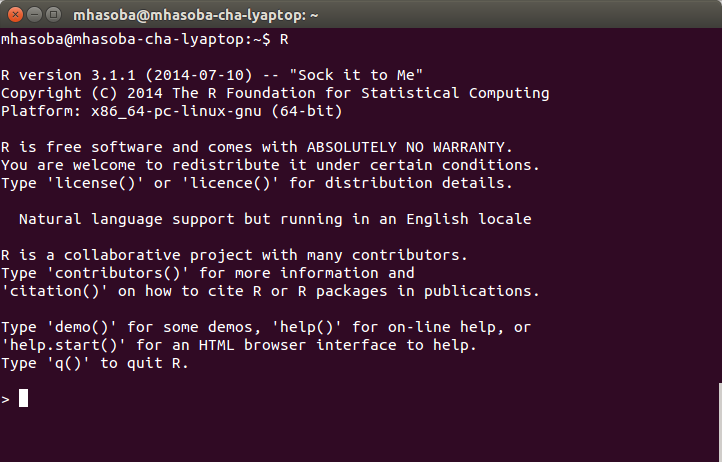
\includegraphics[width=.8\textwidth]{R_Linux.png}
\end{center}

Or like this (Windows "console", similar in Mac):
 
\begin{center}
	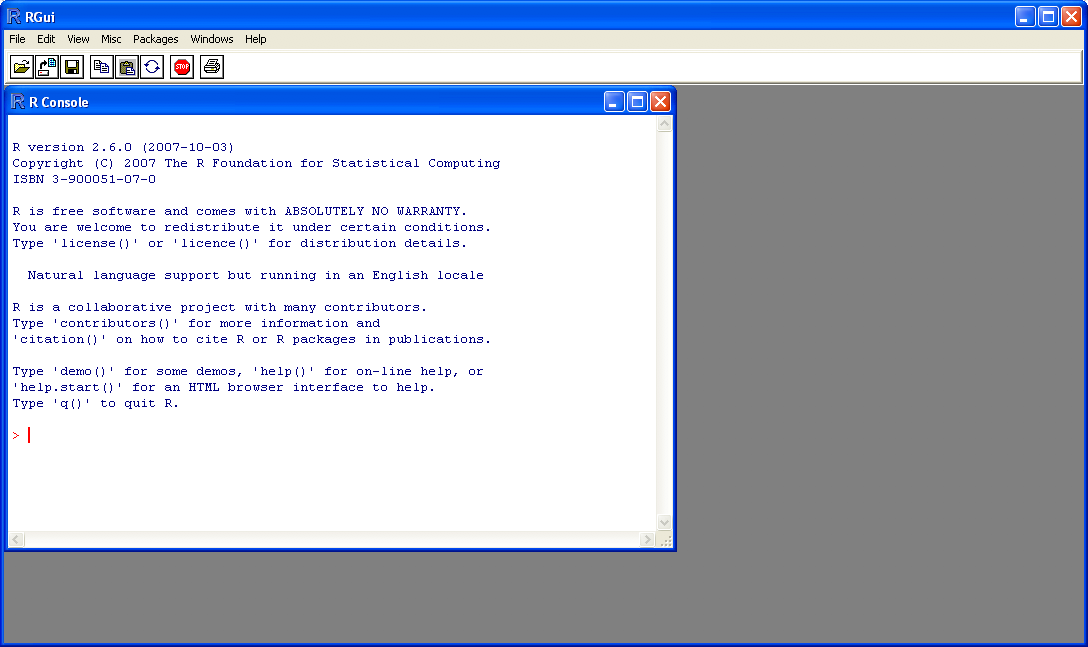
\includegraphics[width=.8\textwidth]{HorrorVacui.png}
\end{center}

\subsection{Gooey IDEs!}

To develop your R code, you should ideally use an IDE (Interactive 
Development Environment) that offers useful features like syntax  
highlighting (google it!) and embedded data and plot viewing windows, 
such as RStudio, {\tt geany}, {\tt vim}, etc. 

These IDEs come with graphic user interfaces (GUI's, or ``gooeys'') of 
differing levels of sophistication and shiny-ness.

In fact, one of the reasons that R has become so popular is that there 
are some very nice, freely available GUI IDE's for it where you can 
use your mouse to do certain ``stuff''. 

In particular, \href{http://rstudio.org/}{RStudio} is very good. 

A big advantage of something like RStudio is that you will get ``syntax 
highlighting'' wherein R language elements such as variables, commands, 
and brackets are differently colored. This is very handy and will make 
your R programming far more convenient and error-free. If you are using 
your own desktop/laptop, you can download it freely from 
\url{https://www.rstudio.com/} and install (versions are available for all 
computer platforms). If you are suing a college computer, it should 
already be available.

The R modules do not require you to use RStudio (everything will 
be command line based), but I would recommend that you to use it, or 
some other IDE like {\tt geany} or {\tt emacs}. 

You may now launch RStudio (assuming it is available on your computer). 
Here is an example RStudio window: 
\begin{center}
	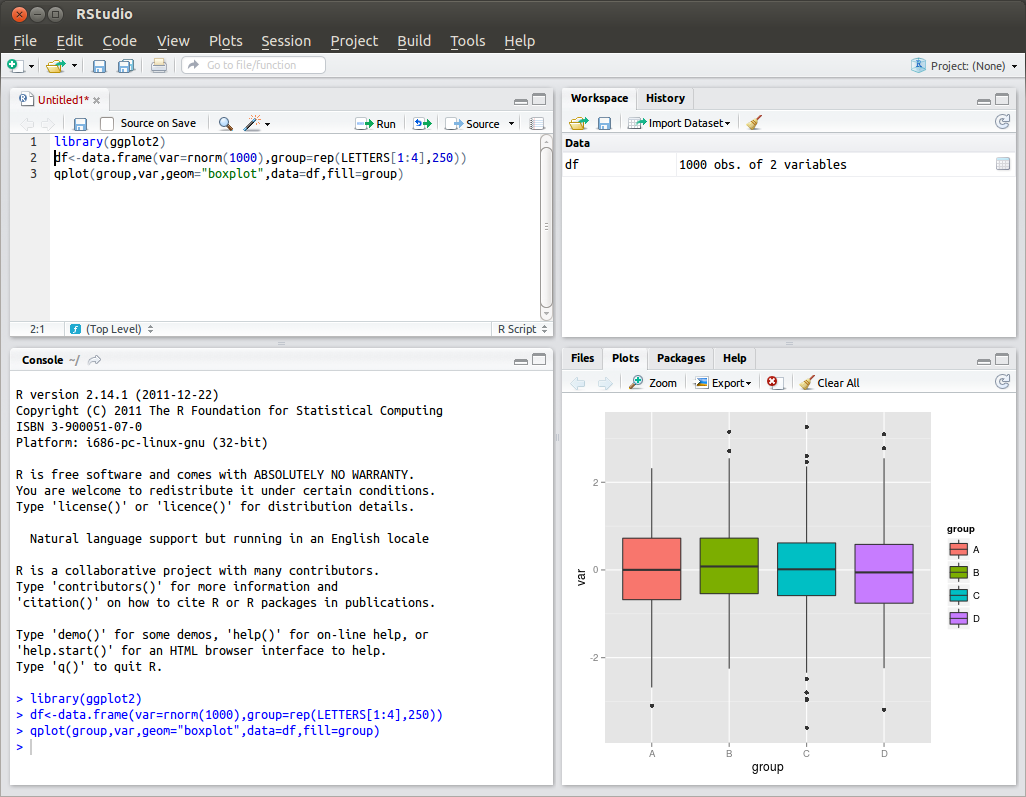
\includegraphics[width=0.8\textwidth]{RStudio.png}
\end{center}

You are still in the R environment, but with some useful frills and 
additional thrills. There are four main elements here (you can hide or 
resize any of them using the RStudio GUI options):

\begin{description}

\item [Console] This is the same R terminal you saw above. In this week 
we will work mainly in this console

\item [Source code] This panel is the code editor with syntax 
highlighting and other handy features that we will explore soon. This 
is where you will write your scripts/programs, and save them. To save, 
you will use {\tt Ctrl + S} and to execute it you will use {\tt Ctrl + Shift + 
S}

\item [Environment] This panel lists all the variables you created 
(more on this later). It has another tab that shows you the history of 
the commands you typed

\item [Plots] This panel shows you all the plots you drew. Other tabs 
in this panel allow you to access the list of packages
you have loaded, and the help page for commands (just type {\tt 
help(command\_name)} in the Console) and packages
\end{description}

In RStudio, you can feed your mouse habit, but I strongly suggest using 
the terminal/console, and resist, to the extent possible, the 
temptation to do everything using the shiny buttons you see (that is 
the dark side pulling, my young {\it padawan}).

\section{Some {\tt R} Basics}

Gets get started with some {\tt R} basics. You will be working by 
entering R commands interactively at the R user prompt ({\tt >}). Up 
and down arrow keys scroll through your command history. 

\subsection{Useful R commands}
\begin{tabular}{p{3cm} p{10cm}} 
	{\tt ls()} & list all the variables in the work space \\
	{\tt rm('a', 'b')} & remove variable(s) {\tt a} and {\tt b}\\
	{\tt rm(list=ls())} & remove all variable(s)\\
	{\tt getwd()} & get current working directory \\
	{\tt setwd('Path')} & set working directory to {\tt Path} \\
	{\tt q()} & quit R \\
	{\tt ?Command} & show the documentation of {\tt Command} \\
	{\tt ??Keyword} & search the all packages/functions with 
	{\tt Keyword}, ``fuzzy search''\\
\end{tabular}\\

\subsection{R Warm-up}

Like in any programming language, you will need to use ``variables'' to 
store information in a R session's workspace. Each Variable has a 
reserved location in your memory (RAM), and takes up ``real estate'' in 
it --- that is when you create a variable you reserve some space in yur 
computer's memory.

Now, try assigning a few variables in the R and doing things to them:
\begin{lstlisting}
> a <- 4  # store 4 as variable a
> a
[1] 4
> a*a  # product
[1] 16
> a_squared <- a*a 
> sqrt(a_squared) # square root
[1] 4
> v <- c(0, 1, 2, 3, 4) # build a vector with c (for "concatenate") 
\end{lstlisting}

Note that any text after a "\#" is ignored by R --- handy for 
commenting. {\it In general, please comment your code and scripts, for 
{\it everybody's} sake}. You will be amazed by how difficult it is to 
read and understand what a certain R script does (or any other script, 
for that matter) without judicious comments --- even scripts you  
yourself wrote not so long ago!

\begin{tipbox}
{\tt c()} (concatenate) is one of the most commonly used 
functions --- it will appear again and again! (try {\tt ?c}). 
\end{tipbox}

OK continuing our R warmup:
\begin{lstlisting}
> v # Display the vector variable you created
[1] 0 1 2 3 4
> is.vector(v) # check if it's a vector
[1] TRUE
> mean(v) # mean
[1] 2
\end{lstlisting}

\begin{tipbox}
Thus, a ``vector'' is like a single column or row in a ``spreadsheet''. Multiple vectors can be combined to make a matrix (the full spreadsheet).  
\end{tipbox}

This is one of many ways R stores and processes data. More on R data 
types and objects below.  

A single value (any kind) is a vector object of length 1 by default. 
That's why in the console you see {\tt [1]} before any single-value 
output (e.g., type {\tt 8}, and you will see {\tt [1] 8}).

\begin{lstlisting}
> var(v) # variance
[1] 2.5
> median(v) # median
[1] 2
> sum(v) # sum all elements
[1] 10
> prod(v + 1) # multiply
[1] 120
> length(v) # length of vector
[1] 5
\end{lstlisting}

\subsection{Variable names and Tabbing}

In R, you can name variables in the following way to keep track of 
related variables:
\begin{lstlisting}
> wing.width.cm <- 1.2 #Using dot notation 
> wing.length.cm <- c(4.7, 5.2, 4.8)
\end{lstlisting}

This can be handy; type:
\begin{lstlisting}
> wing.
\end{lstlisting}

And then hit the {\tt tab} key to reveal all variables in that 
category. This is nice --- variable names should be as obvious as 
possible. However, they should not be over-long either! Good style and 
readability is more important than just convenient variable names. 

\subsection{Operators}
The usual ``operators'' are available in R:

\begin{tabular}{p{2cm} p{11cm}} 
 {\tt +} & Addition \\
 {\tt -} & Subtraction\\
 {\tt *} & Multiplication\\
 {\tt /} & Division\\
 {\tt \textasciicircum} & Power\\
 {\tt \%\%} & Modulo\\
 {\tt \%/\%} & Integer division\\
 {\tt ==} & Equals\\
 {\tt !=} & Differs\\
 {\tt $>$} & Greater\\
 {\tt $>$=} & Greater or equal\\
 {\tt \&} & Logical and\\
 {\tt $\vert$} & Logical or\\
 {\tt !} & Logical not\\
\end{tabular}

\subsection{When things go wrong}

Syntax errors are those where you've just made a mistake while typing 
code. Here are some common problems in {\tt R}: 

\begin{itemize}
\item missing close bracket leads to  continuation line.
\begin{lstlisting}
> x <- (1 + (2 * 3)
+ 
\end{lstlisting}
Hit {\tt Ctrl-C} (UNIX terminal or base R command line) or ESC (in in RStudio) or keep typing!

\item Too many parentheses: {\tt 2 + (2*3))}

\item Wrong or mismatched brackets (see next subsection)

\item Do not mix double quotes and single quotes

\end{itemize}

\begin{tipbox}
	When things are taking too long and the R consile seems frozen, try 
	{\tt Ctrl + C} (UNIX terminal or base R command line) or ESC (in in RStudio) to force an exit from whatever is going on.
\end{tipbox}

\subsection{Types of parentheses}
R has specific uses for different types of parentheses that you need to 
get used to:

\begin{tabular}{p{5cm} p{9.5cm}} 
 {\tt f(3,4)} & call the function (or command) f, with the 
	arguments 3 \& 4. \\
 {\tt a + (b*c)} & to enforce order over which statements 
  or calculations are executed. Here {\tt (b*c)} is executed before 
  adding to {\tt a}; here is an alternative order: {\tt (a + b)*c}\\
 {\tt \{ expr1; expr2; \ldots exprn \}} & group a set of expressions or 
 commands into one compound expression. Value returned is value of last
    expression; used in building function, loops, and conditionals (more on 
    these soon!).\\
 {\tt x[4] } & get the 4th element of the vector {\tt x}.\\
 {\tt li[[3]]} & get the 3rd element of some list {\tt li}, and return it.
    (compare with li[3], which returns a list with just the 3rd element
    inside). More on lists in next section
\end{tabular}

\section{Variable Types}

There are different kinds of data variable types in R, but you will 
basically need to know four for most of your work: integer, float (or 
``numeric'', including real numbers), string (or ``character'', e.g., 
text), and Boolean (``logical''; {\tt True} or {\tt False}).  Try this:

\begin{lstlisting}
> v <- TRUE
> class(v)
[1] "logical"

> v <- 3.2
> class(v)
[1] "numeric"

> v <- 2L
> class(v)
[1] "integer"

> v <- "A string"
> class(v)
[1] "character"
\end{lstlisting}

\begin{tipbox}
R will use {\tt E} notation in outputs of statistical tests to display 
very large or small numbers. If you are not used to different 
representations of long numbers, the {\tt E} notation might be 
confusing. Try this:
\begin{lstlisting}
> 1E4
[1] 10000
> 1e4
[1] 10000
> 5e-2
[1] 0.05
> 1E4^2
[1] 1e+08
> 1 / 3 / 1e8
[1] 3.333333e-09
\end{lstlisting}
Keep and eye out for {\tt E} notation! 
\end{tipbox}

\subsection{Type Conversion and Special Values}
In the following examples, the {\tt as.*} commands all convert a 
variable from one type to another:	
\begin{lstlisting}
> as.integer(3.1)
[1] 3
> as.numeric(4)
[1] 4
> as.roman(155)
[1] CLV
> as.character(155) # same as converting to string
[1] "155"
> as.logical(5) #what's happening here?!
[1] TRUE
> as.logical(0)
[1] FALSE
> b <- NA
> is.na(b)
[1] TRUE
> b <- 0/0
> b
[1] NaN
> is.nan(b)
[1] TRUE
> b <- 5/0
> b
[1] Inf
> is.nan(b)
[1] FALSE
> is.infinite(b)
[1] TRUE
> is.finite(b)
[1] FALSE
> is.finite(0/0)
[1] FALSE
\end{lstlisting}

\begin{tipbox}	
Beware of the difference between {\tt NA} ({\tt N}ot {\tt A}vailable) 
and {\tt NaN} ({\tt N}ot {\tt a} {\tt N}umber)!

R will use {\tt NA} to represent/identify missing values in data or 
outputs, while  {\tt NaN} represent nonsense values (e.g., 0/0) that 
cannot be represented as a number or some other data type. See what R 
has to say about this: try {\tt ?is.nan}, {\tt ?is.na}, {\tt ?NA}, {\tt 
?NaN} in the R commandline (one at a time!).

There are also {\tt Inf} (Infinity, e.g., 1/0), and {\tt NULL} 
(variable not set) value types. Look these up as well using {\tt ?}.
\end{tipbox}

\section{Data Structure types}
R comes with different built-in structures (objects) for data storage and 
manipulation. Mastering these, and knowing which one to use when will 
help you write better, more efficient programs and also handle diverse 
datasets (numbers, counts, names, dates, etc). 

\subsection{Vectors}
The Vector, which you first saw above, is a fundamental data object in 
R. Scalars (single data values) are treated as vector of length 1. {\it 
A vector is like a single column or row in a spreadsheet.} Now get back 
into R (if you somehow quit R using {\tt q()} or something else), and 
try this:
\begin{lstlisting}
> a <- 5
> is.vector(a)
[1] TRUE
> v1 <- c(0.02, 0.5, 1)
> v2 <- c("a", "bc", "def", "ghij")
> v3 <- c(TRUE, TRUE, FALSE)
\end{lstlisting}
{\tt R} vectors can only store data of a single type (e.g., all numeric 
or all character). If you try to combine different types, R will 
homogenize everything to the same data type. To see this, try the 
following:
\begin{lstlisting}
> v1 <- c(0.02, TRUE, 1)
> v1 # TRUE gets converted to 1.00!
[1] 0.02 1.00 1.00
> v1 <- c(0.02, "Mary", 1)
> v1 # Everything gets converted to text!
[1] "0.02" "Mary" "1"
\end{lstlisting}

\subsection{Matrices and arrays} 

A {\tt R} {\tt matrix} is a 2 dimensional vector (has both rows and columns). 
and an {\tt R array} is can store data in more than two dimensions 
(e.g., a stack of 2-D matrices). 

{\tt R} has many functions to build and manipulate matrices and arrays. 
Try:

\begin{lstlisting}	
> mat1 <- matrix(1:25, 5, 5)
> mat1
	 [,1] [,2] [,3] [,4] [,5]
[1,]    1    6   11   16   21
[2,]    2    7   12   17   22
[3,]    3    8   13   18   23
[4,]    4    9   14   19   24
[5,]    5   10   15   20   25
> mat1 <- matrix(1:25, 5, 5, byrow=TRUE)
> mat1
	 [,1] [,2] [,3] [,4] [,5]
[1,]    1    2    3    4    5
[2,]    6    7    8    9   10
[3,]   11   12   13   14   15
[4,]   16   17   18   19   20
[5,]   21   22   23   24   25
> dim(mat1) #get the size of the matrix
[1] 5 5
\end{lstlisting}

Make an array consisting of two 5$\times$5 matrices containing the 
integers 1--50:
\begin{lstlisting}
> arr1 <- array(1:50, c(5, 5, 2))
> arr1
, , 1

	 [,1] [,2] [,3] [,4] [,5]
[1,]    1    6   11   16   21
[2,]    2    7   12   17   22
[3,]    3    8   13   18   23
[4,]    4    9   14   19   24
[5,]    5   10   15   20   25

, , 2

	 [,1] [,2] [,3] [,4] [,5]
[1,]   26   31   36   41   46
[2,]   27   32   37   42   47
[3,]   28   33   38   43   48
[4,]   29   34   39   44   49
[5,]   30   35   40   45   50
\end{lstlisting}

Just like {\tt R} vectors, {\tt R} matrices and arrays have to be of a 
homogeneous type, and R will do the same sort of type homogenization 
you saw for R vectors above (try inserting a text value in {\tt mat1} and 
see what happens), and in {\tt python}'s {\tt numpy} array and matrix 
data structures. 

\subsection{Data frames}

This is a very important data structure in {\tt R}. Unlike matrices and 
vectors, {\tt R} data frames can store data in which each column 
contains a different data type (e.g., numbers, strings, boolean) or 
even a combination of data types, just like a standard spreadsheet. 
Indeed, the dataframe data type was built to emulate some of the 
convenient properties of spreadsheets. Many statistical and plotting 
functions and packages in R naturally use data frames. Let's build and 
manipulate a dataframe:
\begin{lstlisting}
> Col1 <- 1:10
> Col1
 [1]  1  2  3  4  5  6  7  8  9 10
> Col2 <- LETTERS[1:10]
> Col2
 [1] "A" "B" "C" "D" "E" "F" "G" "H" "I" "J"
> Col3 <- runif(10) # 10 random numbers from a uniform distribution
> Col3
 [1] 0.29109 0.91495 0.64962 0.95503 0.26589 0.02482 0.59718
 [8] 0.99134 0.98786 0.86168
> MyDF <- data.frame(Col1, Col2, Col3)
> MyDF
	 Col1 Col2      Col3
1     1    A 0.2910981
2     2    B 0.9149558
3     3    C 0.6496248
4     4    D 0.9550331
5     5    E 0.2658936
6     6    F 0.0248217
7     7    G 0.5971868
8     8    H 0.9913407
9     9    I 0.9878679
10   10    J 0.8616854
> names(MyDF) <- c("A.name", "another", "another.one")
> MyDF
	 A.name another another.one
1       1       A   0.2910981
2       2       B   0.9149558
3       3       C   0.6496248
4       4       D   0.9550331
5       5       E   0.2658936
6       6       F   0.0248217
7       7       G   0.5971868
8       8       H   0.9913407
9       9       I   0.9878679
10     10       J   0.8616854
\end{lstlisting}

Unlike matrices, you can access the contents of data frames by naming 
the columns using a \$ sign: 
\begin{lstlisting}
> MyDF$A.name
 [1]  1  2  3  4  5  6  7  8  9 10
> MyDF[,1] #using numerical indexing instead
 [1]  1  2  3  4  5  6  7  8  9 10
> MyDF[c("A.name","another")] # show two specific columns only
	 A.name another
1       1       A
2       2       B
3       3       C
4       4       D
5       5       E
6       6       F
7       7       G
8       8       H
9       9       I
10     10       J
\end{lstlisting}

You can check whether a particular object is a dataframe data structure with:
\begin{lstlisting}
> class(MyDF)
[1] "data.frame"
\end{lstlisting}
You can check the structure of a dataframe with {\tt str()}:
\begin{lstlisting}
> str(MyDF)
'data.frame':	10 obs. of  3 variables:
 $ A.name     : int  1 2 3 4 5 6 7 8 9 10
 $ another    : Factor w/ 10 levels "A","B","C","D",..
 $ another.one: num  0.291 0.915 0.65 0.955 0.266 ...
\end{lstlisting}
You can print the column names and top few rows with {\tt head()},
\begin{lstlisting}
> head(MyDF)
\end{lstlisting}

And the bottom few rows with {\tt tail()},
\begin{lstlisting}
> tail(MyDF)
\end{lstlisting}

\begin{tipbox}
	What is the ``factor'' data type in the data frame you created? You 
	will see that R may mysteriously convert certain columns in dataframes 
	to a factor type, which has "levels".  
	
	R has a special data type called `factor'. It basically considers 
	columns containing strings-only in a data frame to be a grouping 
	variable. You can convert vectors to and from the {\tt factor} class. 
	Try the following:
	
	\begin{lstlisting}
	> a <- as.factor(2)
	> a
	[1] 2
	Levels: 2
	> class(a)
	[1] "factor"
	\end{lstlisting}	
\end{tipbox}

\subsection{Lists} 

A list is used to collect a group of data objects of different sizes 
and types (e.g., one whole data frame and one vector can both be in a 
single list). It is simply an ordered collection of objects (that can 
be variables). The outputs of many statistical functions in R are lists 
(e.g. linear model fitting using {\tt lm()}), to return all relevant 
information in one output object. So you need to know how to unpack and 
manipulate lists. 

\begin{tipbox}	
As a budding multilingual quantitative biologist, you should not be 
perturbed by the fact that a {\tt list} is a very different data structure in 
python vs R!
\end{tipbox}
	
\begin{lstlisting}
> List1 <- list(species=c("Quercus robur","Fraxinus excelsior"), age=c(123, 84))
> List1
$species
[1] "Quercus robur"      "Fraxinus excelsior"

$age
[1] 123 84
\end{lstlisting}

You can access contents of a list item using number of the item instead of name:
\begin{lstlisting}
> List1[[1]]  
[1] "Quercus robur"      "Fraxinus excelsior"
> List1[[2]]
[1] 123 84
\end{lstlisting}

And you can access it using the name of the item in these two way:
\begin{lstlisting}
> List1[["age"]]
[1] 123 84
> List1$age
[1] 123 84
\end{lstlisting}

You can build lists of lists too! Also, you have perhaps guessed by now 
that {\tt R} dataframes are actually a kind of list.

\begin{tipbox}
If dataframes are so nice, why use {\tt R} matrices at all? The problem 
is that dataframes can be too slow when large numbers of mathematical 
calculations or operations need to be performed. In such cases, you 
will need to convert a dataframe to a matrix. But for statistical 
analyses and plotting, data frames will get the job done.          
\end{tipbox}

\section{Creating and manipulating data structures}
 
\subsection{Creating Sequences}

The {\tt :} operator creates vectors of sequential integers:

\begin{lstlisting}
> years <- 1990:2009
> years
[1] 1990 1991 1992 1993 1994 1995 1996 1997 1998 1999
[11] 2000 2001 2002 2003 2004 2005 2006 2007 2008 2009

> years <- 2009:1990 # or in reverse order 
> years
[1] 2009 2008 2007 2006 2005 2004 2003 2002 2001 2000
[11] 1999 1998 1997 1996 1995 1994 1993 1992 1991 1990
\end{lstlisting}

For sequences of fractional numbers, you have to use {\tt seq()} :

\begin{lstlisting}
> seq(1, 10, 0.5)
 [1]  1.0  1.5  2.0  2.5  3.0  3.5  4.0  4.5  5.0  5.5  6.0  6.5  7.0  7.5  8.0
[16]  8.5  9.0  9.5 10.0
\end{lstlisting}

You can also {\tt seq(from=1,to=10, by=0.5)} OR {\tt seq(from=1, 
by=0.5, to=10)} with the same effect (try it) --- this explicit, 
"argument matching" approach is partly why {\tt R} is so popular.

\subsection{Acessing parts of data stuctures -- Indices and Indexing}
Every element (entry) of a vector in R has an order: the first value, 
second, third, etc. To illustrate this, let's create a simple vector:
\begin{lstlisting}
> MyVar <- c( 'a' , 'b' , 'c' , 'd' , 'e' )
\end{lstlisting}
Then, square brackets extract values based on their numerical order 
in the vector:
\begin{lstlisting}
> MyVar[1] # Show element in first position 
[1] "a"
> MyVar[4]
[1] "d" # Show element in fourth position 
\end{lstlisting}
The values in square brackets are called "indices" --- they 
give the index (position) of the required value. We can also select 
sets of values in different orders, or repeat values:
\begin{lstlisting}
> MyVar[c(3,2,1)] # reverse order
[1] "c" "b" "a"
MyVar[c(1,1,5,5)] # repeat indices
[1] "a" "a" "e" "e"
\end{lstlisting}

You can also manipulate data structures/objects by indexing:

\begin{lstlisting}
> v <- c(0, 1, 2, 3, 4) # Re-create the vector variable v
> v[3] # access one element
[1] 2
> v[1:3] # access sequential elements
[1] 0 1 2
> v[-3] # remove elements
[1] 0 1 3 4
> v[c(1, 4)] # access non-sequential
[1] 0 3
\end{lstlisting}

For matrices, you need to use both row and column indices:
\begin{lstlisting}	
> mat1 <- matrix(1:25, 5, 5, byrow=TRUE) #create a matrix
> mat1
	 [,1] [,2] [,3] [,4] [,5]
[1,]    1    2    3    4    5
[2,]    6    7    8    9   10
[3,]   11   12   13   14   15
[4,]   16   17   18   19   20
[5,]   21   22   23   24   25
> mat1[1,2]
[1] 2
> mat1[1,2:4]
[1] 2 3 4
> mat1[1:2,2:4]
	 [,1] [,2] [,3]
[1,]    2    3    4
[2,]    7    8    9
\end{lstlisting}

\subsection{Recycling}
When vectors are of different lengths, {\tt R} will recycle the shorter 
one to make a vector of the same length:
\begin{lstlisting}
a <- c(1,5) + 2
x <- c(1,2); y <- c(5,3,9,2)
x + y
x + c(y,1)  ## somewhat strange!
\end{lstlisting}

Recycling is convenient, but dangerous!

\subsection{Basic vector-matrix operations}

\begin{lstlisting}
> v <- c(0, 1, 2, 3, 4)
> v2 <- v*2 # multiply whole vector by 2
> v2
[1] 0 2 4 6 8
> v * v2 # element-wise product
[1]  0  2  8 18 32
> t(v) # transpose the vector
	 [,1] [,2] [,3] [,4] [,5]
[1,]    0    1    2    3    4
> v %*% t(v) # matrix/vector product
	 [,1] [,2] [,3] [,4] [,5]
[1,]    0    0    0    0    0
[2,]    0    1    2    3    4
[3,]    0    2    4    6    8
[4,]    0    3    6    9   12
[5,]    0    4    8   12   16
> v3 <- 1:7 # assign using sequence
> v3
[1] 1 2 3 4 5 6 7
> v4 <- c(v2, v3) # concatenate vectors
> v4
 [1] 0 2 4 6 8 1 2 3 4 5 6 7
\end{lstlisting}

\subsection{Strings and Pasting}
It is important to know how to handle strings in R for two main reasons:
\begin{compactitem}
	\item To deal with text data, such as names of experimental 
	treatments 
	\item To generate appropriate text labels and titles for figures 
\end{compactitem}

Let's try creating and manipulating strings:
\begin{lstlisting}
> species.name <- "Quercus robur" #double quotes
> species.name
[1] "Quercus robur"
> species.name <- 'Fraxinus excelsior' #single quotes 
> species.name
[1] "Fraxinus excelsior"
> paste("Quercus", "robur")
[1] "Quercus robur"
> paste("Quercus", "robur",sep = "") #Get rid of space
"Quercusrobur"
> paste("Quercus", "robur",sep = ", ") #insert comma to separate
\end{lstlisting}
As you can see above, both double and single quotes work, but I suggest 
that you use double quotes --- this will allow you to define strings 
that contain a single quotes, which is often necessary.

And as is the case with so many R functions, pasting works on vectors:
\begin{lstlisting}
> paste('Year is:', 1990:2000)
 [1] "Year is: 1990" "Year is: 1991" "Year is: 1992" "Year is: 1993"
 [5] "Year is: 1994" "Year is: 1995" "Year is: 1996" "Year is: 1997"
 [9] "Year is: 1998" "Year is: 1999" "Year is: 2000"
\end{lstlisting}

Note that this last example creates a vector of 11 strings as it is 
1990:2000 {\it inclusive}. 

\begin{tipbox}
{\it Data ``structures'' vs. ``objects'' in {\tt R}}:\\

You will often see the terms ``object'' and ``data structure'' thrown 
around this week and elsewhere. These two have a very distinct meaning 
in object-oriented programs (OOPs) like {\tt R}. The main thing you 
need to keep in mind is that a data structrure is just a ``dumb'' 
container for data (e.g., a vector). An object, on the other hand can 
be a data structure, but also any other variables or functions in your R 
environment. R, being an OOP, needs to convert everything in the 
current environment to an object so that it knows what to do with each 
such entity --- each object type has its own set of rules for operations and 
manipulations that R uses when interpreting your commands. 

If all this sounds like gobbledygook, don't worry too much!      
	
\end{tipbox}

\section{Your analysis workflow}

In using {\tt R} for an analysis, you will likely use and create 
several files. As in the case of {\tt bash} and {\tt python} based 
projects, in {\tt R} projects as well, you should keep your workflow 
well organized. For example, it is sensible to create a folder 
(directory) to keep all code files together. You can then set {\tt R} 
to work from this directory, so that files are easy to find and run --- 
this will be your ``working directory'' (more on this below). Also, you 
don't want to mix code files with data and results files. So you should 
create separate directories for these as well. Thus, your typical {\tt 
R} analysis workflow will be:

\begin{center}
\begin{tikzpicture}[bx/.style={draw=green!30!black, rectangle, very thick, rounded corners, 
	                           minimum height=20pt, minimum width=4cm, text depth=0pt},
                    zn/.style={rectangle, rounded corners, fill=black!10, minimum width=5 cm, minimum height=5cm},
                    lb/.style={right=0pt, yshift=7pt, font=\small, green!30!black},
                    every path/.style={-stealth, very thick, green!30!black}]

	\node (R)       {
\includegraphics[width=2cm]{R_logo.png}};                    
	\node (inputs)  [zn, left= of R] {};
	\node (outputs) [zn, right= of R] {};
	\node (lab)     [lb, at=(inputs.north west), black] {Input files};
	\node (lab)     [lb, at=(outputs.north west), black] {Output files (all to {\tt Results})};

	\node (Rin)     [bx, above=1cm of inputs.center, anchor=center] {MyScript.R};
	\node (data)    [bx, below=1cm of inputs.center, anchor=center] {MyData.csv};
	
	\node (lab)     [lb, at=(Rin.north west)] {R script file (from {\tt Code})};
	\node (lab)     [lb, at=(data.north west)] {Text data file (from {\tt Data})} ;

	\node (Results) [bx, at=(outputs.center)]{MyTextResults.txt};
	\node (image)   [bx, above=1.5cm of outputs.center, anchor=center]{MyGraphicResults.pdf};
	\node (Rdata)   [bx, below=1.5cm of outputs.center, anchor=center]{MyRData.Rda};

	\node (lab)     [lb, at=(Results.north west)] {Results output};
	\node (lab)     [lb, at=(image.north west)] {Graphics file};
	\node (lab)     [lb, at=(Rdata.north west)] {R data file};

	\draw [bend left, shorten > = -8pt] (Rin.east) to (R);
	\draw [bend right, shorten > = -8pt](data.east) to (R);

	\draw [bend left, shorten < = -1pt]  (R) to (image.west);
	\draw [bend right, shorten < = -1pt, stealth-stealth] (R) to (Rdata.west);
	\draw (R) -- (Results.west);

\end{tikzpicture}
\end{center}

Some details on each kind of file:
\begin{description}

\item [R script files] These are plain text files containing all the R 
code needed for an analysis. These should always be created with a 
simple text editor like Notepad (Windows), TextEdit (MacOS) or Geany 
(Linux) and saved with the extension {\tt *.R}. We will use RStudio in 
this class (more on this below). You should {\it never} use Word to 
save or edit these files as R can only read code from plain text files. 
 
\item [Text data files] These are files of data in plain text format 
containing one or more columns of data (numbers, strings, or both). 
Although there are several format options, we will tyoucally be using 
csv files, where the entries are separated by commas. These are easy to 
create and export from Excel (if that's what you use...).\footnote{If 
you are using a computer from elsewhere in the EU, Excel may use a 
comma ($\pi=3,1416$) instead of a decimal point ($\pi=3.1416$). In this 
case, {\it csv} files may use a semi-colon to separate columns and you 
can use the alternative function {\it read.csv2()} to read them into 
R.} 

\item [Results output files] These are a plain text files contain your 
results, such the the summary of output of a regression or ANOVA  
analysis. Typically, you will putput your results in a table format 
where the columns are separated by commas (csv) or tabs 
(tab-delimited) 

\item [Graphics files] R can export graphics in a wide range of 
formats. This can be done automatically from R code and we will look at 
this later but you can also select a graphics window and click `File 
$\triangleright$ Save as...'

\item [Rdata files] You can save any data loaded or created in R, 
including model outputs and other things, into a single{\tt Rdata} 
file. These are not plain text and can only be read by R, but can hold 
all the data from an analysis in a single handy location. I never use 
these, but you can, if you want.  

\end{description}

So let's build your {\tt R} analysis project structure. 

Do the following:
\begin{compactitem}[$\quad\star$]
	\item Create a sensibly named directory (e.g., {\tt MyICRModule}, {\tt Week3}, etc in an 
	appropriate location on your computer. If you are using a college Windows 
	computer, you will need to create it in your {\tt H:} drive.  
	 
	\item Create subdirectories {\it within this directory} called {\tt 
	Code}, {\tt Data}, and {\tt Results}
\end{compactitem}

\begin{tipbox}
	Avoid including spaces in your file or directory names, as this will 
	often create problems when you share your file or directory with 
	somebody else. Many software programs do not handle spaces in 
	file/directory names well. Use underscores instead of spaces. For 
	example, instead of {\tt My IC R Module}, use {\tt 
	My\_IC\_R\_Module}.  
	
\end{tipbox}

You can create directories using {\tt dir.create()} within {\tt R}:

\begin{lstlisting}
> dir.create("MyICRModule")
> dir.create("MyICRModule/Code")
> dir.create("MyICRModule/Data")	
> dir.create("MyICRModule/Results")	
\end{lstlisting}

\subsection{The R Workspace and Working Directory}

R has a ``workspace'' -- a current working environment that includes 
any user-defined data structures objects (vectors, matrices, data 
frames, lists) as well as other objects (e.g., functions). At the end 
of an R session, the user can save an image of the current workspace 
that is automatically reloaded the next time R is started. Your 
workspace is saved in your ``Working Directory'', which has to be set 
manually.

So before we go any further, let's get sort out where your R ``Working 
Directory'' should be and how you should set it. R has a default 
location where it assumes your working directory is. 

in Windows, it is {\tt C:/Windows/system32} or similar.

in Mac, it is {\tt /User/User Name} or similar.

In UNIX/Linux, it is whichever directory you are in when you launch R.

To see where your current working directory is, at the R command 
prompt, type:
\begin{lstlisting}
> getwd() 
\end{lstlisting}
This tells you what the current working directory ("{\tt wd}") is. 

Now, set the working directory to be {\tt MyICRModule/Code}. For 
example, if you created {\tt MyICRModule} directly in your {\tt 
H:\textbackslash }, the you would use:
\begin{lstlisting}
> setwd("H:/MyICRModule/Code") 
> dir() #check what's in the current working directory
\end{lstlisting}
On your own computer, you can also change R's default to a particular 
working directory where you would like to start (easily done in RStudio). 

In Linux, you can do this by editing the {\tt Rprofile.site} site with 
\\ {\tt sudo geany /etc/R/Rprofile.site}. In that file, you would add 
your start-up parameters between the lines {\tt .First <- function() 
cat("\textbackslash n   Welcome to R!\textbackslash n\textbackslash 
n")} and {\tt .Last <- function() cat("\textbackslash n   
Goodbye!\textbackslash n\textbackslash n")} --- between these lines, 
insert \\{\tt setwd("/home/YourName/YourDirectoryPath")}

In Windows and Macs, you can find the {\tt Rprofile.site} file by 
searching for it. When I last checked for Windows, it used to be at {\tt 
C:\textbackslash Program Files\textbackslash R\textbackslash 
etc\textbackslash Rprofile.site }

If you are using RStudio, you can change the default working directory 
by through the RStudio "Options" dialog.

\section{Importing and Exporting Data}
We are now ready to see how to import and export data in R, typically 
the first step of your analysis. The best option is to have your data 
in a {\tt c}omma {\tt s}eparated {\tt v}alue ({\tt csv}) text file or 
in a tab separated text file. Then, 
you can use the function {\tt read.csv} (or {\tt read.table}) to import 
your data. Now, lets get some data into your {\tt Data} directory.

\begin{compactitem}[$\quad\star$]
	\item Go to the repository you downloaded from bitbucket and 
	unzipped, and navigate to the {\tt Data} directory. 
	\item Copy the file {\tt trees.csv} into your own {\tt Data} 
	directory.
	\item Now, try the following:
\end{compactitem}
\begin{lstlisting}
> MyData <- read.csv("../Data/trees.csv")
> ls() #Check that MyData has appeared 
> head(MyData) # Have a quick look at the data frame
> str(MyData) # Have a quick look at the column types
> MyData <- read.csv("../Data/trees.csv", header = TRUE) # with headers
> MyData <- read.table("../Data/trees.csv", sep = ',', header = TRUE) #another way
> head(MyData)
> MyData <- read.csv("../Data/trees.csv", skip = 5) # skip first 5 lines
\end{lstlisting}

Note that the resulting {\tt MyData} in your workspace is a R 
dataframe. Also, note the UNIX-like paths using forward slashes (Windows uses 
back slashes). 

\subsection{Relative paths!} 

The $../$ in {\tt read.csv("../Data/trees.csv")} above signifies a 
"relative" path. That is, you are asking R to load data that lies in a 
different directory (folder) relative your current location (in this 
case, you are in your {\tt Code} directory). In other, more dorky 
words, {\tt ../Data/trees.txt} points to a file named {\tt trees.txt} 
located in the "parent" of the current directory.

{\it What is an absolute path?}--- one that specifies the whole path on 
your computer, say from {\tt C:/} "upwards".  

Using relative paths in in your R scripts and code will make your code 
computer independent and your life better! The relative path way should 
always be the way you load data in your analyses scripts --- it will 
guarantee that your analysis works on every computer, not just your 
college computer. 

Also, {\it AVOID putting a {\tt setwd} command at the start of your R 
script}, as setting the working directory always requires an absolute 
directory path, which will differ across computers, platforms, and 
users. Let the end user sort out how to set the working directory. So 
to import data and export results, your script should {\it not} use 
absolute paths.  

\subsection{Writing out to and saving files}

You can also save your data frames using {\tt write.table} or {\tt 
write.csv}:

\begin{lstlisting}
> write.csv(MyData, "../Results/MyData.csv")
> dir("../Results/") # Check if it worked
> write.table(MyData[1,], file = "../Results/MyData.csv",append=TRUE) # append
> write.csv(MyData, "../Results/MyData.csv", row.names=TRUE) # write row names
> write.table(MyData, "../Results/MyData.csv", col.names=FALSE) # ignore col names
\end{lstlisting}

\section{Writing R code}
 
Typing in commands interactively in the R console is good for starters, 
but you will want to switch to putting your sequence of commands into a 
script file, and then ask R to run those commands. 

\begin{compactitem}[$\quad\star$]
	\item Open a new text file, call it {\tt basic\_io.R}, and save it to 
	your {\tt Code} directory. 
	\item Write the above input-output commands in it: 
\end{compactitem}
\lstinputlisting[language=R]{Practicals/Code/basic_io.R}

You will get a warning with {\tt write.table(MyData[1,], file = 
"../Results/MyData.csv",append=TRUE)} because R thinks it is silly that 
you are appending headers to a file that already has headers!

\begin{compactitem}[$\quad\star$]
	\item Place the cursor on the first line of code in the script file 
	and run it by pressing the keyboard shortcut (PC: ctrl+R, Mac: 
	command+enter, Linux: ctrl+enter if you are using {\tt geany}).
	\item Check after every line that you are getting the expected result.
\end{compactitem}

\subsection{Running R code}

But even writing to a script file and running the code line-by-line or 
block-by-block is not your ultimate goal. What you would really like to 
do is to just run your full analysis and output all the results. There 
are two main approaches for running R script/code.

\subsubsection{Using {\tt source}}


You can run all the contents of a {\tt *.R} script file from the {\tt 
R} command line by using {\tt source}. This causes R to accept code 
input from the named file and run it.
\begin{compactitem}[$\quad\star$]
	\item Try sourcing {\tt basic\_io.R}: 
\end{compactitem}

\begin{lstlisting}
> source("basic_io.R") # Assuming you are in Code directory!
\end{lstlisting}
\begin{compactitem}[$\quad\star$]
	\item If you get errors, fix them!
\end{compactitem}

\begin{tipbox}
Do not put a {\tt source()} command inside the script file you are 
sourcing, as it is then trying to run itself again and again and that's 
just cruel!
\end{tipbox}

Note that you will need to add the directory path to the file name 
({\tt basic\_io.R} in the above example), if the script file is not in 
your working directory. For example, you will need \\{\tt 
source("../Code/control.R"} if your working directory is {\tt Data} and 
not {\tt Code}.

\begin{tipbox}
The command {\tt source()} has a {\tt chdir} argument whose default 
value is FALSE. When set to TRUE, it will change the working directory 
to the directory of the file being sourced.  
\end{tipbox}

\subsubsection{Using {\tt Rscript}}

You can also run R script from the UNIX/Linux terminal by calling {\tt 
Rscript}. You can then easily automate the execution of your R scripts 
(e.g., by writing a bash script) and integrate R into a bigger 
computing pipeline/workflow by calling it through other tools or 
languages (such as {\tt Python}; see Chapter \ref{chap:pythonII}). 

Let's try using {\tt Rscript} to run {\tt basic\_io.R}: 

\begin{compactitem}[$\quad\star$]
	\item Exit from the R console using {\tt ctrl+D}, or open a new 
	bash terminal
	
	\item {\tt cd} to the location of {\tt basic\_io.R} (presumably, {\tt 
	Week3/code})
	
	\item Then run the script using Rscript 
\begin{lstlisting}
$ Rscript basic_io.R 
\end{lstlisting}
	
\end{compactitem}

Also, please have a look at {\tt man Rscript} in a bash terminal.

\begin{tipbox}
Thus, you have to be inside an R session to use {\tt source}, while 
you can only call {\tt Rscript} from the UNIX/Linux terminal.
\end{tipbox}  

\subsubsection{Running R in batch mode}

In addition to {\tt Rscript}, there is another way to run you R script 
without opening the R console. In Mac or linux, you can do so by 
typing:

\noindent {\tt R CMD BATCH MyCode.R MyResults.Rout}

This will create an {\tt MyResults.Rout} file containing all the output. 
On Microsoft Windows, it's more complicated --- change the path to {\tt 
R.exe} and output file as needed: 

\noindent {\tt "C:\textbackslash{}Program 
Files\textbackslash{}R\textbackslash{}R-3.1.1\textbackslash{}bin\textbackslash{}R.exe" 
CMD BATCH --vanilla --slave\\
 "C:\textbackslash{}PathToMyResults\textbackslash{}Results\textbackslash{}MyCode.R"}
  
\section{Writing R Functions}
Like any other programming language, R lets you write your own 
functions. A function is a block of re-useable code that takes an 
input, does something with it (or to it!), and returns the result. All 
the ``commands'' that you have been using, such as {\tt ls()}, {\tt 
mean()}, {\tt c()}, etc are basically functions. You will want to write 
your own function for every scenario where a particular, task or set 
of analysis steps need to be performed again and again.   

The syntax for R functions is quite simple, with each function accepting 
``arguments'' and ``returning'' a value. 

Type the following into a script file called  {\tt boilerplate.R} and 
save it in your {\tt Code} directory.
 
\lstinputlisting[language=R]{Practicals/Code/boilerplate.R}

Note the curly brackets -- these are necessary for R to know where the 
specification of the function starts and ends. Also, note the 
indentation. Not necessary (unlike Python), but recommended to make
code more readable.

Now source the script
\begin{lstlisting}
> source("boilerplate.R")	
\end{lstlisting}
This will run the script, and also save your function {\tt MyFunction} 
as an object into your workspace (try {\tt ls()}, and you will see {\tt 
MyFunction} appear in the list of objects). 

Also try: 
\begin{lstlisting}
> class(MyFunction)
[1] "function"	
\end{lstlisting}
So, yes, {\tt MyFunction} is a {\tt function} object! 

Now let's write an script containing a more useful function:
\begin{compactitem}[$\quad\star$]
	\item In your text editor type the following in a file called {\tt 
	TreeHeight.R}, and save it in your {\tt Code} directory:
\end{compactitem}

\lstinputlisting[language=R]{Practicals/Code/TreeHeight.R}

\begin{compactitem}[$\quad\star$]
	\item Run {\tt TreeHeight.R} block by block and check what each line 
	is doing.
	\item Now run it using {\tt source} and/or {\tt Rscript}.
	\item If you get errors, carefully read the error messages and fix 
	them!
\end{compactitem}

\section{Practicals}

\begin{enumerate}
	
	\item Modify the script {\tt TreeHeight.R} so that it does the following:
	\begin{compactitem}
		
	 \item Loads {\tt trees.csv} and calculates tree heights for all 
	    trees in the data. Note that the distances have been measured in 
	    meters. (Hint: use relative paths))
	    
		\item Creates a csv output file called {\tt TreeHts.csv} in {\tt 
		Results} that contains the calculated tree heights along with the 
		original data in the following format (only first two rows and 
		headers shown):	
	\begin{lstlisting}
	"Species","Distance.m","Angle.degrees","Tree.Height.m"
	"Populus tremula",31.6658337740228,41.2826361937914,25.462680727681
	"Quercus robur",45.984992608428,44.5359166583512,46.094124200205
	\end{lstlisting}

	\item This script should work using either {\tt source} or {\tt 
	Rscript}

	\end{compactitem}

	\item Make the {\tt TreeHeight.R} script more general so that it 
	could be used for other datasets, not just {\tt trees.csv}:
	
	\begin{compactitem}
		
	\item Write another R script called {\tt get\_TreeHeight.R} 
	that takes a csv file name from the command line (e.g., {\tt 
	get\_TreeHeight.R Trees.csv}) and outputs the result to a file just 
	like {\tt TreeHeight.R} above, but this time includes the input file 
	name in the output file name as {\tt InputFileName\_treeheights.csv}. 
	Note that you will have to strip the {\tt .csv} or whatever the 
	extension is from the filename, and also {\tt ../} etc., if you are 
	using relative paths 
	
	(Hint: Command-line parameters are accessible within the R running 
	environment via \\{\tt commandArgs()} --- so help(commandArgs) might 
	be your starting point.)

	\item Write a Unix shell script called {\tt run\_get\_TreeHeight.sh} 
	that tests \\ {\tt get\_TreeHeight.R} --- include {\tt 
	trees.csv} as your example file. Note that 	{\tt source} will not 
	work in this case as it does not allow scripts with arguments to be 
	run; you will have to use {\tt Rscript} instead. 

	\end{compactitem}

	\item {\bf Extra credit}: If you have already started on {\tt python} 
	(Chapter \ref{chap:pythonI}), write a python version of {\tt 
	get\_TreeHeight.R} (call it {\tt get\_TreeHeight.py}). Include a test 
	of this script into {\tt run\_get\_TreeHeight.sh}.	 
\end{enumerate}

\section{Control statements}
In R, you can write {\tt if}, {\tt then}, {\tt else} statements, and 
{\tt for} and {\tt while} loops like any programming language.
However, loops are slow in R, so use them sparingly. Such statements 
are useful to include in functions and scripts because you may only 
want to do certain calculations or otehr tasks, under certain 
conditions (e.g., {\tt if} the dataset is from a particular year, do 
something different). 

\begin{compactitem}[$\quad\star$]
	\item Type the following in a script file called {\tt control.R} 
	(save it in your {\tt Code} directory) 	
	\item Run {\tt control.R} function block by block (not line by line!) 
	and check what each line is doing.
	\item Now run it using {\tt source} and {\tt Rscript}.
	\item If you get errors, fix them (OK, I am going to stop saying this 
	henceforth!).
\end{compactitem}

\lstinputlisting[language=R]{Practicals/Code/control.R}

\section{Useful R Functions}
There are a number of very useful functions available by default (in 
the "base packages"). Here are some particularly useful ones:

\subsection{Mathematical}

\begin{tabular}{p{2.5cm} p{10cm}} 
{\tt log(x)} & Natural logarithm\\
{\tt log10(x)} & Logarithm in base 10\\
{\tt exp(x)} & $e^x$\\
{\tt abs(x)} & Absolute value\\
{\tt floor(x)} & Largest integer $<x$\\
{\tt ceiling(x)} & Smallest integer $>x$\\
{\tt pi} & $\pi$\\
{\tt sqrt(x)} & $\sqrt{x}$\\
{\tt sin(x)} & Sinus function\\
\end{tabular}

\subsection{Strings}

\begin{tabular}{p{4.5cm} p{8cm}}
{\tt strsplit(x,';')} & Split the string at ';' \\
{\tt nchar(x)} & Number of characters\\
{\tt toupper(x)} & Set to upper case\\
{\tt tolower(x)} & Set to lower case\\
{\tt paste(x1,x2,sep=';')} & Join the strings using ';'\\
\end{tabular}

\subsection{Statistical}

\begin{tabular}{p{3.5cm} p{9.5cm}}
	{\tt mean(x)} & Compute mean (of a vector or matrix)\\
	{\tt sd(x)} & Standard deviation\\
	{\tt var(x)} & Variance\\
	{\tt median(x)} & Median\\
	{\tt quantile(x,0.05)} & Compute the 0.05 quantile\\
	{\tt range(x)} & Range of the data\\
	{\tt min(x)} & Minimum\\
	{\tt max(x)} & Maximum\\
	{\tt sum(x)} & Sum all elements\\
\end{tabular}

\section{Packages}
The main strength of R is that users can easily build packages and 
share them through \url{https://cran.r-project.org/}. There are packages to do 
most statistical and mathematical analysis you might conceive, so check 
them out before reinventing the wheel! Visit \url{https://cran.r-project.org/} 
and go to packages to see a list and a brief description. 

In UNIX, you can use the terminal to install R packages:
\begin{lstlisting}
$ sudo apt-get install r-cran-ggplot2 r-cran-plyr r-cran-reshape2
\end{lstlisting}

In Windows and Macs, you can install a package within R by using the 
{\tt install.packages()} command. 

Let's install the following packages:
\begin{lstlisting}
> install.packages(c("ggplot2","plyr","reshape2"))
\end{lstlisting}

You can also use the RStudio GUI to install packages using your mouse 
and menu. 

\begin{tipbox}
In UNIX, you will have to launch a {\tt sudo R} session to get 
installation from within {\tt R} using  {\tt install.packages()} to work 
properly. Otherwise, you be forced to install the package in a 
non-standard location on your drive that does not require {\tt sudo} 
privileges.
\end{tipbox}


\section{Practicals wrap-up}

  \begin{enumerate}

	\item Review and make sure you can run all the commands, code 
	fragments, and named scripts we have built till now and get the 
	expected outputs.

	\item Annotate/comment your code lines as much and as often as necessary 
	using \#.
	
	\item Keep all files organized in {\tt code}, {\tt data} and {\tt 
	results} directories.
	 
   \end{enumerate}

\begin{center}
	\it {\tt git add}, {\tt commit} and {\tt push} all your code and data 
	from this chapter to your git repository by the {\it following 
	Wednesday 5PM}.
\end{center}

\section{Readings}
Check the readings under the R directory in the bitbucket master 
repository! Also, google "R tutorial", and plenty will pop up. Choose 
ones that seem the most intuitive to you.
\begin{itemize}\itemsep2pt
	\item The Use R! series (the yellow books) by Springer are really 
	good. In particular, consider: ``A Beginner's Guide to R'', ``R by 
	Example'', ``Numerical Ecology With R'', ``ggplot2'' (coming up in 
	Chapter \ref{chap:R_data}), ``A Primer of 
	Ecology with R'', ``Nonlinear Regression with R'', ``Analysis of 
	Phylogenetics and Evolution with R''.
	\item For more focus on dynamical models: Soetaert \& Herman. 2009 
	``A practical guide to ecological modelling: using R as a 
	simulation platform''.
	\item There are excellent websites besides cran. In particular, check out 
	\url{https://www.statmethods.net/} and  \url{https://en.wikibooks.org/wiki/R_Programming}. 	
	\item For those who are coming with Matlab experience:
      \url{http://www.math.umaine.edu/~hiebeler/comp/matlabR.html}
  \item Bolker, B. M.: Ecological Models and Data in R (eBook and 
    Hardcover available).
  \item Beckerman, A. P. \& Petchey, O. L. (2012) Getting started 
    with R: an introduction for biologists. Oxford, Oxford University 
    Press. \\ Very basic, good if you are really stuck at the outset. 
  \item Crawley, R. (2013) The R book. 2nd edition. Chichester, Wiley. \\
    Excellent but enormous reference book, code and data available from
    \url{www.bio.ic.ac.uk/research/mjcraw/therbook/index.htm}
	
\end{itemize}

\chapter{Advanced topics in {R}}
\label{chap:R_II}

In this chapter, you will learn some additional topics in R to
\begin{itemize}
	\item Make data wrangling, analyses, and simulations 
	more efficient using vectorization and tools such as {\tt plyr}

	\item Use some advanced tools for control flows and looping
	
	\item Generate random numbers for statistical simulations and looping
	
	\item Find and fix errors in R code using debugging 

	\item Become aware of some additional tools and topics in R 
	(accessing databases, building your own packages, etc.). 
	
\end{itemize}

\section{Vectorization}
R is very slow at running cycles ({\tt for} and {\tt while} loops). 
This is because R is a ``nimble'' language: at execution time R does 
not know what you'are going to perform until it ``reads'' the code to 
perform. Compiled languages such as {\tt C}, know exactly what the flow 
of the program is, as the code is ``compiled'' before execution. 

As a metaphor, {\tt C} is a musician playing a score she has seen 
before -- optimizing each passage, while R is playing it ``a prima 
vista'' (i.e., at first sight) -- this can slow code execution and 
operations down. Let's see an example that illustrates this point.

\begin{compactitem}[$\quad\star$]
		\item Type (save in {\tt Code}) as {\tt Vectorize1.R} the following
		script, and run it (it sums all elements of a matrix):
\end{compactitem}

\lstinputlisting[language=R]{Practicals/Code/Vectorize1.R}

Note the {\tt system.time} R function --- it calculates how much time 
your code takes.

Both {\tt SumAllElements()} and {\tt sum()} approaches are correct, and 
will give you the right answer. However, the inbuilt function {\tt 
sum()}  is 100 times faster than the other, because it is uses 
vectorization that avoids the amount of looping that {\tt 
SumAllElements()} uses!

\begin{tipbox}
	In R, even if you should try to avoid loops, in practice, it is often 
	much easier to throw in a {\tt for} loop, and {\it then} ``optimize'' 
	the code to avoid the loop if the running time is not 
	satisfactory. Therefore, it won't hurt you to become really familiar 
	with loops and looping as you learned in Chapter \ref{chap:RI}  
\end{tipbox} 

Fortunately, R has several functions that can operate on entire vectors 
and matrices without requiring looping (Vectorization). That is, 
vectorizing a computer program means you write it such that as many 
operations as possible are applied to whole data structure (vectors, 
matrices, dataframes, lists, etc) at one go, instead of its individual 
elements. 

Let's learn about some important R functions that allow vectorization 
in the following sections.

\subsection{The {\tt *apply} family of functions}

There are a family of functions called {\tt *apply} in R that vectorize 
your code for you. These functions are described in the help files (e.g. 
{\tt ?apply}). 

For example, {\tt apply} can be used when you want to apply a function 
to the rows or columns of a matrix (and higher-dimensional analogues -- 
remember arrays!). This is not generally advisable for data frames as 
it will first need to coerce the data frame to a matrix first.

\begin{compactitem}[$\quad\star$]
\item Type the following in a script file called {\tt apply1.R}, save 
it to your {\tt Code} directory, and run it:
\end{compactitem}

\lstinputlisting[language=R]{Practicals/Code/apply1.R}

That was using apply on some of R's inbuilt functions. You can use 
apply to define your own functions. Let's try it.
\begin{compactitem}[$\quad\star$]
\item Type the following in a script file called {\tt apply2.R}, save 
it to your {\tt Code} directory, and run it:
\end{compactitem}

\lstinputlisting[language=R]{Practicals/Code/apply2.R}

There are many other methods: {\tt lapply}, {\tt sapply}, {\tt eapply}, 
etc. Each is best for a given data type. For example, {\tt lapply} is 
best for R lists. Have a look at {\scriptsize
\url{https://stackoverflow.com/questions/3505701/grouping-functions-tapply-by-aggregate-and-the-apply-family}} 
for some guidelines. 

\subsubsection{The {\tt tapply} function}
We will look at {\tt tapply}, which is particularly useful because it 
allows you to apply a function to subsets of a vector in a dataframe, 
with the subsets defined by some other vector in the same dataframe, 
usually a factor (this could be useful for your Chapter \ref{chap:R_data} 
pound hill data analysis, for example!). 

This makes it a bit of a different member of the {\tt *apply} family.  
Try this:
\begin{lstlisting}
> x <- 1:20 # a vector

# A factor (of the same length) defining groups:
> y <- factor(rep(letters[1:5], each = 4)) 

# Add up the values in x within each subgroup defined by y:
> tapply(x, y, sum)  
 a  b  c  d  e 
10 26 42 58 74
\end{lstlisting}
 
\subsection{Using {\tt by}}

You can also do something similar to {\tt tapply} with the {\tt by} 
function, i.e., apply a function to a dataframe using some factor to 
define the subsets. Try this:

\begin{lstlisting}
## import some data
attach(iris)
print (iris)

## use colMeans (as it is better for dataframes)
by(iris[,1:2], iris$Species, colMeans)
by(iris[,1:2], iris$Petal.Width, colMeans)
\end{lstlisting}

\subsection{Using {\tt replicate}}

The {\tt replicate} function is useful to avoid a loop for function 
that typically involves random number generation (more on this below). 
For example:

\begin{lstlisting}
> print(replicate(10, runif(5))) 
\end{lstlisting}
This generates a 10 $\times$ 5 matrix of uniformly distributed random 
numbers. 

\subsection{Using {\tt plyr} and {\tt ddply}}

The {\tt plyr} package combines the functionality of the {\tt *apply} 
family, into a few handy functions. Look up 
\url{http://plyr.had.co.nz/}.

In particular, {\tt ddply} is very useful, because for each subset of a 
data frame, it applies a function and then combines results into 
another data frame (very useful for Practical \ref{sec:PPPrac2} in Chapter 
\ref{chap:R_data}!). In other words, ``ddply '' means: take a data frame, 
split it up, do something to it, and return a data frame.  

Look up \url{http://seananderson.ca/2013/12/01/plyr.html} and 
\url{https://www.r-bloggers.com/transforming-subsets-of-data-in-r-with-by-ddply-and-data-table/} 
for examples.	There you will also see a comparison of speed of {\tt 
ddply} vs {\tt by} at the latter web page--- {\tt ddply} is actually 
slower than other vectorized methods, as it trades-off compactness of 
use for some of the speed of vectorization! Indeed, overall functions 
in {\tt plyr} can be slow if you are working with very large datasets 
that involve a lot of subsetting (analyses by many groups or grouping 
variables). 

\begin{tipbox}
The base {\tt *apply} functions remain useful and worth 
knowing even if you do get into {\tt plyr} or better still, {\tt 
dplyr} (see Chapter \ref{chap:R_data})
\end{tipbox}

\section{Some more control flow tools}

Let's look at some more control tools, which we first learned about in 
Chapter \ref{chap:RI}.  

\subsection{{\tt break}ing out of loops}
Often it is useful (or necessary) to {\tt break} out of a loop when 
some condition is met. Use {\tt break} (like in pretty much any other 
programming language, like {\tt python}) in situations when you cannot 
set a target number of iterations, as you would with a {\tt while} loop 
(Chapter 1). Try this (type into {\tt break.R} and save in {\tt Code}):

\lstinputlisting[language=R]{Practicals/Code/break.R}

\subsection{Using {\tt next}}
You can also skip to next iteration of a loop. Both {\tt next} and {\tt 
break} can be used within other loops ({\tt while}, {\tt for}). Try 
this (type into {\tt next.R} and save in {\tt Code}):

\lstinputlisting[language=R]{Practicals/Code/next.R}

This script checks if a number is odd using the ``modulo'' 
operation and prints if it is.

\begin{tipbox}
{\bf Reminder}: Indent your code! Indentation helps you see 
the flow of the logic, rather than flattened version, which is hard for 
you and everybody else to read. I recommend using the {\it tab} key to 
indent.
\end{tipbox}

\section{Practicals}

\begin{enumerate}
	
\item {\bf A vectorization challenge}

The Ricker model is a classic discrete population model which was 
introduced in 1954 by Ricker to model recruitment of stock in fisheries.
It gives the expected number (or density) $N_{t+1}$ of individuals in 
generation $t + 1$ as a function of the number of individuals in the 
previous generation $t$:
\begin{equation}
N_{t+1} = N_t e^{r\left(1-\frac{N_t}{k}\right)}
\end{equation} 
Here $r$ is intrinsic growth rate and $k$ as the 
carrying capacity of the environment. Try this script that runs it:

\lstinputlisting[language=R]{Practicals/Code/Ricker.R}

Now open and run the script {\tt Vectorize2.R} (available on the 
bitbucket repository). This is the stochastic Ricker model (compare 
with the above script to see where the stochasticity (random error) 
enters). Now modify the script to complete the exercise given. 
 
{\it You will be marked on this one based upon how much faster your solution 
is compared to mine!}

\item {\bf Extra Credit:} Implement the python versions of {\tt 
Vectorize1.R} and {\tt Vectorize2.R} (call them {\tt 
Vectorize1.py} and {\tt Vectorize2.py} respectively). Then write a bash 
script that compares the computational speed of the four scripts. the 
bash script should display meaningful summary of the results in the 
terminal.       
 

\end{enumerate}

\section{Generating Random Numbers}

You will probably need to generate random numbers at some point in your 
journey towards becoming a proper data analyst or quantitative 
biologist. 

R has many routines for generating random samples from various 
probability distributions --- we have already used {\tt runif()}, {\tt 
rnorm()}. There are a number of random number distributions that you can sample 
or generate random numbers from: 

\begin{tabular}{p{5.4cm} p{9cm}}
	{\tt rnorm(10, m=0, sd=1)} & Draw 10 normal random numbers with mean 0 and s.d. 1\\
	{\tt dnorm(x, m=0, sd=1)} & Density function\\
	{\tt qnorm(x, m=0, sd=1)} & Cumulative density function\\
	{\tt runif(20, min=0, max=2)} & Twenty random numbers from uniform
			[0,2]\\
	{\tt rpois(20, lambda=10)} & Twenty random numbers from
			Poisson($\lambda$)\\
\end{tabular}\\

\subsection{``Seeding'' random number generators}   
Before proceeding further, note that computers don't really generate mathematically random numbers, but 
instead a sequence of numbers that are close to random: ``pseudo-random 
numbers''. They are generated based on some iterative formula:

\[ x_{new} = f( x_{old}) \mod N \]

where modulo operation provides the ``remainder'' division.

So to generate the first random number, you need a {\bf seed}. Setting 
the seed allows you to reliably generate the same sequence of numbers, 
which can be useful when debugging programs (next section). 

Now, try this:

\begin{lstlisting}
> set.seed(1234567)
> rnorm(1)
 0.1567038
\end{lstlisting}

What happened?! If this were truly a random number, how would everybody 
get the same answer? Now try {\tt rnorm(10)} and compare the results 
with your neighbour. Thus "random" numbers generated in R and in any 
other software are in fact "deterministic", but from a very complex 
formula that yields numbers with properties like random numbers. 

Effectively, {\tt rnorm} has an enormous list that it cycles through. 
The random seed starts the process, i.e., indicates where in the list 
to start. This is usually taken from the clock when you start R.

But why bother with this? Well, for debugging (next section). Bugs in 
code can be hard to find --- harder still if you are generating random 
numbers, so repeat runs of your code may or may not all trigger the 
same behaviour. You can set the seed once at the beginning of the code 
--- ensuring repeatability, retaining (pseudo) randomness. Once 
debugged, if you want, you can remove the set seed line.

To try out how sampling works, type the following into {\tt sample.R} 
and save in {\tt Code}:

\lstinputlisting[language=R]{Practicals/Code/sample.R}

\section{Errors and Debugging}

\subsection{"Catching" errors}

Often, you don't know if a simulation or a R function will work on a 
particular data or variable, or a value of a variable (can happen in 
many stats functions). 

Indeed, as most of you must have already experienced by now, there can 
be frustrating, puzzling bugs in programs that lead to mysterious 
errors. Often, the error and warning messages you get are 
un-understandable, especially in R! 

Rather than having R throw you out of the code, you would rather catch 
the error and keep going. This can be done using {\tt try}. Modify {\tt 
sample.R} as follows the 
following into {\tt try.R} and save in {\tt Code} (what does this 
script do?):

\lstinputlisting[language=R]{Practicals/Code/try.R}

Note the functions {\tt sample} and {\tt stop} in the above script.  
Also check out {\tt tryCatch}.

\subsection{Debugging}

Once you have found an error, you would like to fix it. This is called 
debugging. Here are some useful debugging functions in R : 

\begin{itemize}\itemsep2pt

\item Warnings vs Errors; converting warnings to errors: {\tt 
stopifnot()} --- a bit like {\tt try}

\item What to do when you get an error: {\tt traceback()}

\item Simple {\tt print} commands in the right places can be useful 
for testing (but not strongly recommended)

\item Use of {\tt browser()} at key points in code --- my favourite option 
(also look up  {\tt recover()})

\item {\tt debug(fn)}, {\tt undebug(fn)} : More technical approach to 
debugging --- explore them
\end{itemize}

Let's look at an example using {\tt browser()}. {\tt browser()} is 
handy because it will allow you to "single-step" through your code. 
Place it within your function at the point you want to examine (e.g.) 
local variables. 

Here's an  example usage of {\tt browser()} (type in {\tt browse.R} and 
save in {\tt Code}):

\lstinputlisting[language=R]{Practicals/Code/browse.R}

Now, within the browser, you can enter expressions as 
normal, or you can use a few particularly useful debug commands:
\begin{itemize}
\item {\tt n}: single-step 
\item {\tt c}: exit browser and continue
\item {\tt Q}: exit browser and abort, return to top-level.
\end{itemize}

\section{Building your own R packages} 

You can packaging up your code, data sets and documentation to make a 
{\it bona fide} R package. You may wish to do this for particularly 
large projects that you think will be useful for others. Read {\it 
Writing R Extensions} 
(\url{cran.r-project.org/doc/manuals/r-release/R-exts.html} manual and 
see {\it package.skeleton} to get started. The R tool set EcoDataTools 
(\url{https://github.com/DomBennett/EcoDataTools}) and the package 
{\tt cheddar} were written by Silwood Grad Students! 
        
\section{Sweave and knitr}

Sweave and knitr are tools that allows you to write your Dissertation 
Report or some other document such that it can be updated automatically 
if data or R analysis change. Instead of inserting a prefabricated 
graph or table into the report, the master document contains the R code 
necessary to obtain it. When run through R, all data analysis output 
(tables, graphs, etc.) is created on the fly and inserted into a final 
document, which can be written using \LaTeX, LyX, HTML, or Markdown. 
The report can be automatically updated if data or analysis change, 
which allows for truly reproducible research. Check out 
\url{https://support.rstudio.com/hc/en-us/articles/200552056-Using-Sweave-and-knitr} and 
\url{http://yihui.name/knitr/}.

\section{Practicals} 

\begin{enumerate}
	
\item Autocorrelation in weather (this Practical may make more sense 
once you have done the R and Stats week where you will learn about 
correlation coefficients and p-values).

\begin{compactitem}[$\quad\star$]
		
\item Make a new script named {\tt TAutoCorr.R}, and save in {\tt Code}
directory
  
\item At the start of the script, load and examine and plot \\ {\tt 
KeyWestAnnualMeanTemperature.Rdata}, using {\tt load()} --- This is the 
temperature in Key West, Florida for the 20th century.

\item {\bf The question this script will help answer is}: Is the 
temperature of one year significantly correlated with the next year 
(successive years), {\it across the years}. That us you will be 
calculating the correlation between $n-1$ pairs of years, where $n$ is 
the total number of years. However, you can't use the standard p-value 
calculated for a correlation coefficient (using {\tt R}'s {\tt cor()} 
function -- see below) because measurements of climatic variables in 
successive time-points in a time series (successive seconds, minutes, 
hours, months, years, etc.) are {\it not independent}.

\item Therefore,
\begin{enumerate}\itemsep0pt
\item Compute the appropriate correlation coefficient between successive 
years and store it (look at the help file for {\tt cor()}
\item Then repeat this calculation 10000 times by\\ 
-- randomly permuting the time series (Hint: you can use the {\tt 
sample} function that we learned about in this Chapter --- read the 
help file for this function and experiment with it),\\
-- then computing the correlation coefficient for each randomly permuted 
year sequence and storing it\\
\end{enumerate}

\item Then calculate what fraction of the correlation coefficients from 
step 2 were greater than that from step 1 (this is your approximate 
p-value).

\item {\it How do you interpret these results? Why? Present your 
results and their interpretation in a pdf document written in \LaTeX 
(please include the the document's source code as well).}

\end{compactitem}

\item{Mapping} (Extra Credit)

Your project may not really need GIS, but you may still like/need to do 
some mapping. You you can do it in R using the {\tt maps} package. In 
this practical, you will map the Global Population Dynamics Database 
(\url{https://www.imperial.ac.uk/cpb/gpdd/gpdd.aspx}) (GPDD). This is a 
freely available database that was developed at Silwood). 

If any of you are interested in doing a project around this database, 
please contact David Orme or Samraat Pawar! It is a gold mine of as yet 
under-utilized information. Note that the Living Planet Index 
(\url{http://livingplanetindex.org/home/index}) is based upon these 
data.

\begin{compactitem}[$\quad\star$]
\item Use {\tt load()} from {\tt GPDDFiltered.RData} that is available 
on the bitbucket git repository --- have a look at the database field headers and 
contents. 
\item What you need is latitude and longitude information for a bunch of 
species for which population time series are available in the GPDD
\item Now use {\tt install.packages()} to install the package {\tt 
maps}, as you did with {\tt ggplot2} --- hopefully without any 
problems!
\item Now create a script (saved under a sensible name in a sensible 
location --- hint hint!) that:
	\begin{enumerate}\itemsep0pt
		\item Loads the maps package
		\item Loads the GPDD data
		\item Creates a world map (use the map function, read its help 
		file, also google examples using {\item maps})
		\item  Superimposes on the map all the locations from which we have 
		data in the GPDD dataframe
		\item Compare your map with a fellow student to check
	\end{enumerate}

\item {\it Based on this map, what biases might you expect in any analysis 
based on the data represented? --- {\it include your answer as a comment at 
the end of your R script}. } 
\end{compactitem}

\end{enumerate}

\section{R Module Wrap up}
 
 \subsection{Some comments and suggestions}

Thanks for enduring through the week! Learning to program in R or any 
other language, especially if it's your first-ever effort to learn 
programming, demands perseverance. Y'all have shown admirable 
quantities of this necessary quality. Keep going! I believe most if not 
all of you have climbed a significant part of a steep learning curve. 
Here are some things to keep in mind:

\begin{itemize}\itemsep2pt

\item There are many R nerds at Silwood that you can talk to --- {\it 
They walk among us!}

\item There is a Silwood R list that you can subscribe to: 
\url{https://mailman.ic.ac.uk/mailman/listinfo/silwood-r}

\item However, post questions only as a last resort! Google it first, 
and even before that, make sure you revise this week's (and stats 
week's) work.

\item Solutions to this weeks Practicals will become available by 15th 
Nov.

\end{itemize}

\section{Practicals wrap-up}

  \begin{enumerate}

	\item Review and make sure you can run all the commands, code 
	fragments, and named scripts we have built till now and get the 
	expected outputs.

	\item Annotate/comment your code lines as much and as often as 
	necessary using \#.
	
	\item Keep all code, data and results files organized in the {\tt 
	Week3/} directory
	 
   \end{enumerate}

\begin{center}
	\it {\tt git add}, {\tt commit} and {\tt push} all your code and data 
	from this chapter to your git repository by Wednesday, Nov 2, 5PM.
\end{center}

\section{Readings}

\begin{itemize}
    
	\item See {\bf An introduction to the Interactive Debugging Tools in R,
	Roger D Peng} for detailed usage. 
	\url{http://www.biostat.jhsph.edu/~rpeng/docs/R-debug-tools.pdf}
	
	\item Friedrich Leisch. (2002) Sweave: Dynamic generation of statistical 
	reports using literate data analysis. Proceedings in Computational 
	Statistics, pages 575-580. Physica Verlag, Heidelberg, 2002. 
	\url{http://www.statistik.lmu.de/~leisch/Sweave}
	
	\item Remember, R packages come with pdf guides/documentation!
	
\end{itemize}


\chapter{Data exploration and visualization}
\label{chap:R_data}

\epigraph{Clutter and confusion are failures of design, not attributes 
of information.}{\textit{Edward Tufte}}

Before you do any fancy statistical analyses with data, you must clean, 
explore, and visualize it. And eventually, you want to produce a 
finished product that presents visualizations you data and your results 
clearly and concisely. Ultimately, both, at the data exploration and the 
finished product stages, the goal of graphics is to present information 
such that it provides intuitive ideas. As Edward Tufte says: 
\begin{quote} \it
``Graphical excellence is that which gives to the viewer the greatest 
number of ideas in the shortest time with the least ink in the smallest 
space.'' 
\end{quote}

This chapter aims at introducing you to principles, and R packages and 
commands that will allow you to build a computational pipeline/workflow 
for critical steps of your data analysis and visualization. 

We will start with some basic plotting and data exploration. Then, you 
will learn to generate publication-quality graphics using the {\tt 
ggplot2} package. Finally, you will learn some principles and methods 
for data processing and storage in R. 

\section{Basic plotting and graphical data exploration}

R can produce beautiful graphics without the time-consuming and fiddly 
methods that you might have used in Excel or equivalent. You should 
also make it a habit to quickly plot the data for exploratory analysis. 
So we are going to learn some basic plotting first. 

\subsection{Basic plotting commands} 

Here is a menu of basic R plotting commands (use {\tt ?commandname} to 
learn more about it):

\begin{tabular}{p{3.1cm} p{10cm}} 
{\tt plot(x,y)} & Scatterplot\\
{\tt plot(y$\sim$x)} & Scatterplot with {\tt y} as a response variable \\
{\tt hist(mydata)} & Histogram\\
{\tt barplot(mydata)} & Bar plot\\
{\tt points(y1$\sim$x1)} & Add another series of points\\
{\tt boxplot(y$\sim$x)} & Boxplot\\
\end{tabular}\\

\subsection{R graphics devices}

In all that follows, you may often end up plotting multiple plots on 
the same graphics window without intending to do so, because R by 
default keeps plotting in the most recent plotting window that was 
opened. You can close a particular graphics window or "device" by using 
{\tt dev.off()}, and all open devices/windows with {\tt 
graphics.off()}. By default, {\tt dev.off()} will close the most recent 
figure device that was opened. 

\begin{tipbox}
Note that there are invisible devices in {\tt R}! Fore example, if you are 
	printing to pdf (coming up below), the device or graphics window will 
	not be visible on your computer screen. 
\end{tipbox}

Now let's try some simple plotting for data exploration. As a 
case study, we will use a dataset on Consumer-Resource (e.g., 
Predator-Prey) body mass ratios taken from the Ecological Archives of 
the ESA (Barnes {\em et al.} 2008, Ecology 89:881).

\begin{compactitem}[$\quad\star$]
	\item Copy the file {\tt EcolArchives-E089-51-D1.csv} from {\tt Data} directory in the master git repository on bitbucket to your own {\tt Data} directory. 
	\item Now, launch R and read in these data to a data frame:
\begin{lstlisting}
> MyDF <- read.csv("../Data/EcolArchives-E089-51-D1.csv")
> dim(MyDF) #check the size of the data frame you loaded
[1] 34931    15
\end{lstlisting}
\end{compactitem}

Let's look at what the data contain (type {\tt MyDF\$} and hit the TAB 
key twice (if you are using RStudio, you just can hit it once). This will give the following result: 
\begin{lstlisting}
> MyDF$
MyDF$Record.number                MyDF$Predator.mass
MyDF$In.refID                     MyDF$Prey
MyDF$IndividualID                 MyDF$Prey.common.name
MyDF$Predator                     MyDF$Prey.taxon
MyDF$Predator.common.name         MyDF$Prey.mass
MyDF$Predator.taxon               MyDF$Prey.mass.unit
MyDF$Predator.lifestage           MyDF$Location
MyDF$Type.of.feeding.interaction  
\end{lstlisting}
{\bf In RStudio, you will see a drop-down list of all the column 
headers when you hit {\tt tab}}.

You can also use the {\tt str()} and {\tt head()} commands that you 
learned about in Chapter \ref{chap:RI}.

As you can see, these data contain predator-prey body size information. 
This is an interesting dataset because it is huge, and covers a wide 
range of body sizes of aquatic species involved in consumer-resource 
interactions --- from unicells to whales. Analyzing this dataset should 
tell us a lot about what sizes of prey predators like to eat.

\begin{figure} \centering
   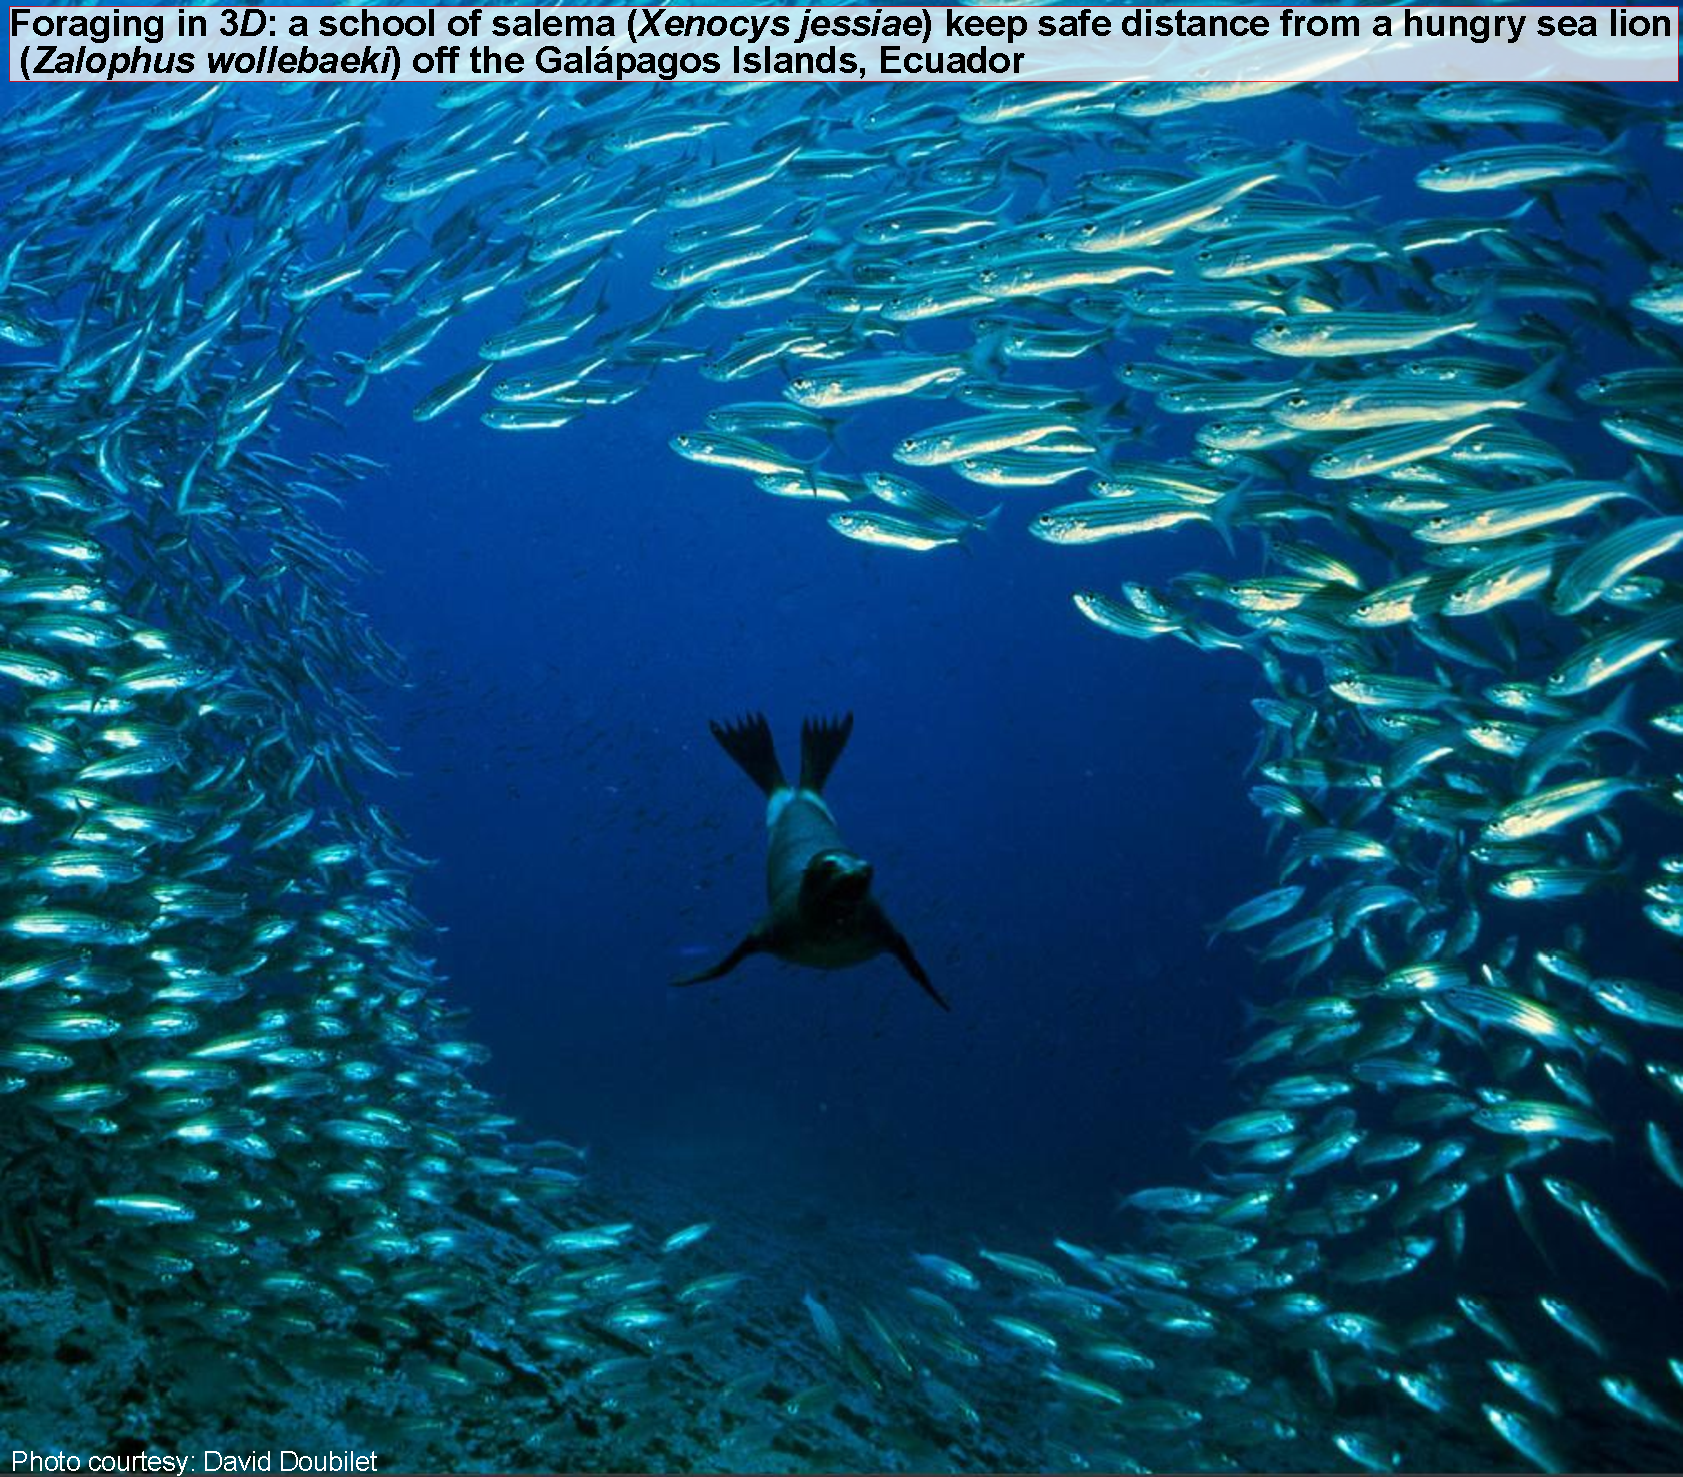
\includegraphics[width=0.8\textwidth]{SeaLion.pdf} 
	 \caption{A consumer-resource (predator-prey) interaction waiting to 
	 happen.}
\end{figure}

\subsection{Scatter Plot}

Let's start by plotting Predator mass vs. Prey mass:
\begin{lstlisting}
> plot(MyDF$Predator.mass,MyDF$Prey.mass)
\end{lstlisting}
\begin{center}
   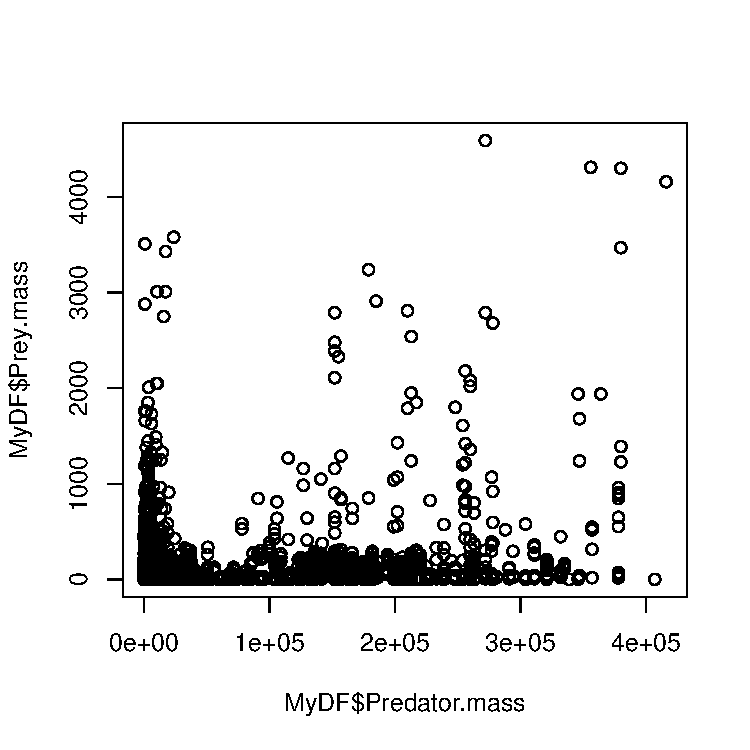
\includegraphics[width=0.5\textwidth]{PPScat1.pdf} 
\end{center}

That doesn't look very nice! Let's try taking logarithms (why?). 

\begin{lstlisting}
> plot(log(MyDF$Predator.mass),log(MyDF$Prey.mass))
\end{lstlisting}
\begin{center}
   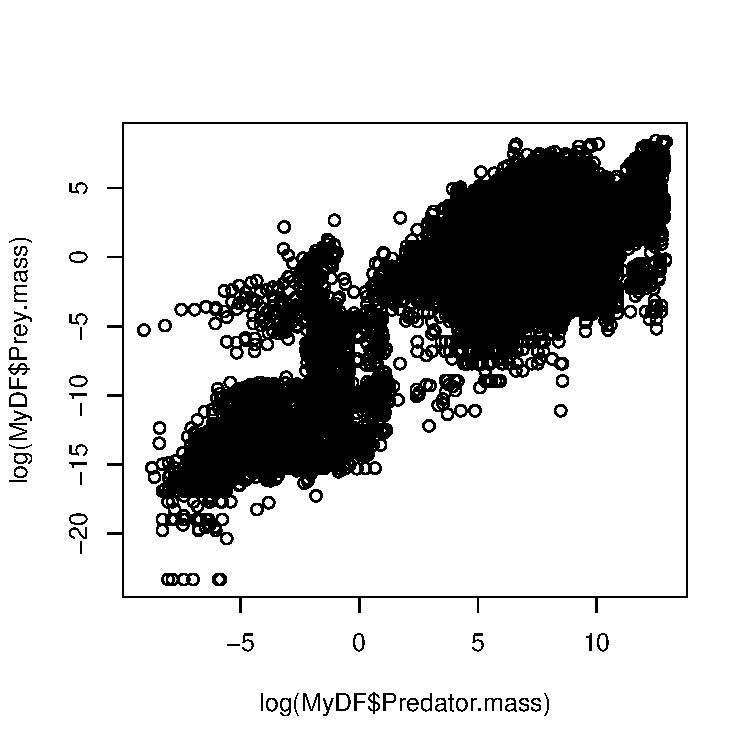
\includegraphics[width=0.5\textwidth]{PPScat2.pdf} 
\end{center}
We can change almost any aspect of the resulting graph; let's change the
symbols by specifying the {\tt p}lot {\tt ch}aracters using {\tt pch}:

\begin{lstlisting}
> plot(log(MyDF$Predator.mass),log(MyDF$Prey.mass),pch=20) # Change marker
\end{lstlisting}
\begin{center}
   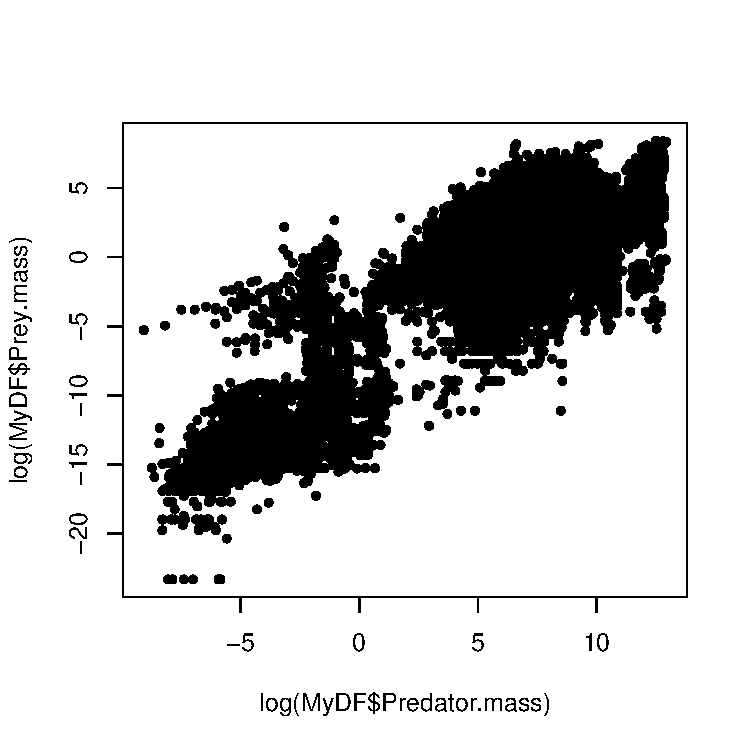
\includegraphics[width=0.5\textwidth]{PPScat3.pdf} 
\end{center}

\begin{lstlisting}
> plot(log(MyDF$Predator.mass),log(MyDF$Prey.mass),pch=20,
    xlab = "Predator Mass (kg)", ylab = "Prey Mass (kg)") # Add labels
\end{lstlisting}
\begin{center}
   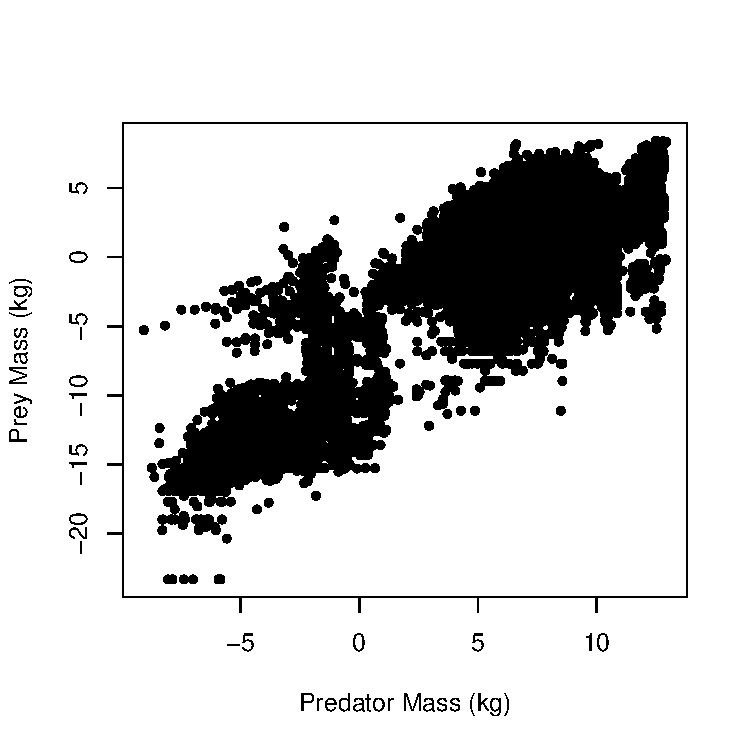
\includegraphics[width=0.5\textwidth]{PPScat4.pdf} 
\end{center}

\begin{tipbox}
	A really great summary of basic R graphical parameters can be found 
	at \url{https://www.statmethods.net/advgraphs/parameters.html}
\end{tipbox}

\subsection{Histograms}
Why did we have to take a logarithm to see the relationship between 
predator and prey size? Plotting histograms of the two classes 
(predator, prey) should be insightful, as we can then see the 
``marginal'' distributions of the two variables. 

Let's first plot a histogram of predator body masses:
\begin{lstlisting}
> hist(MyDF$Predator.mass)
\end{lstlisting}
\begin{center}
   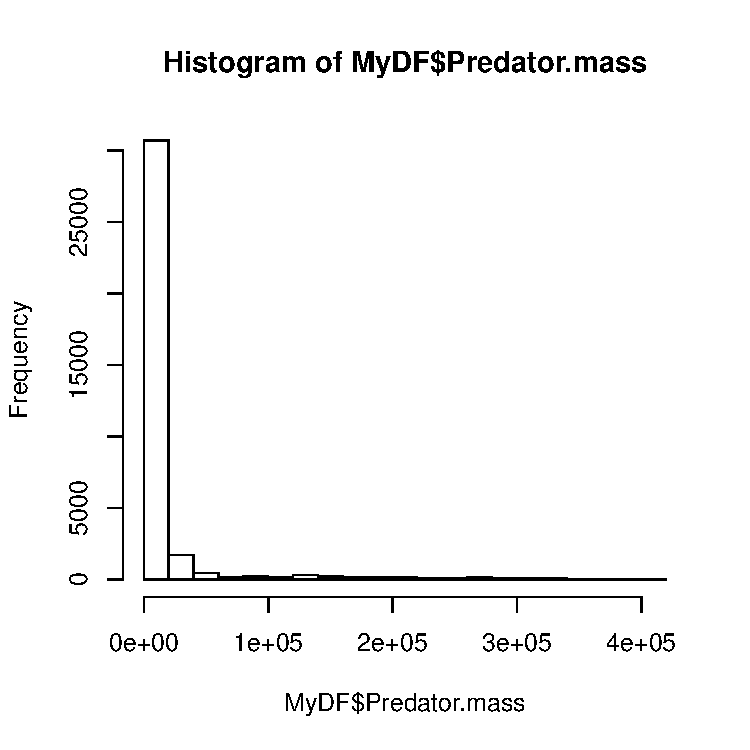
\includegraphics[width=0.5\textwidth]{PrHist1.pdf} 
\end{center}

Clearly, the data are heavily right skewed, with small body sized organisms 
dominating (that's a universal pattern on planet earth). Let's now take 
a logarithm and see if we can get a better idea of what the 
distribution of predator sizes looks like:
\begin{lstlisting}
> hist(log(MyDF$Predator.mass), 
   xlab = "Predator Mass (kg)", ylab = "Count") # include labels
\end{lstlisting}
\begin{center}
   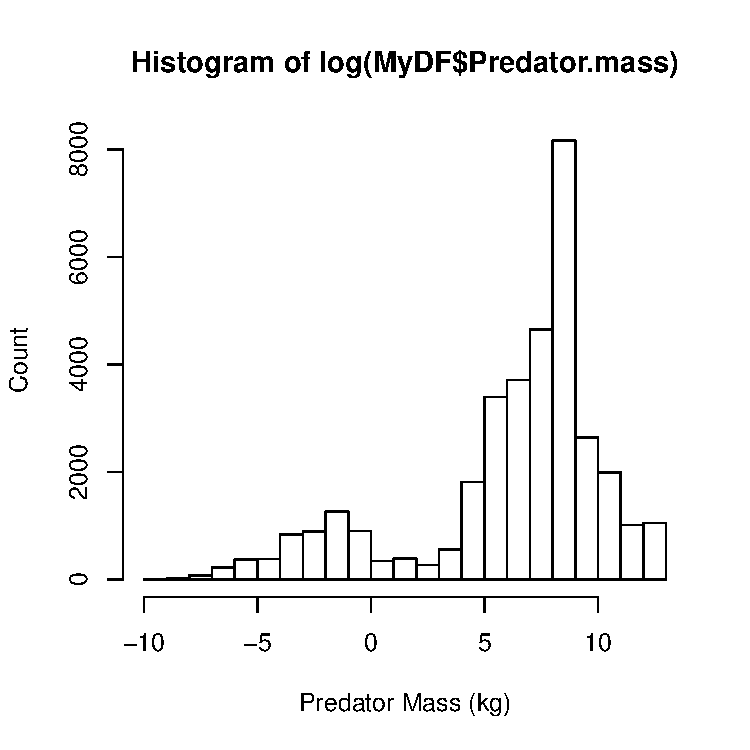
\includegraphics[width=0.5\textwidth]{PrHist2.pdf} 
\end{center}

\begin{lstlisting}
> hist(log(MyDF$Predator.mass),xlab="Predator Mass (kg)",ylab="Count", 
    col = "lightblue", border = "pink") # Change bar and borders colors 
\end{lstlisting}
\begin{center}
   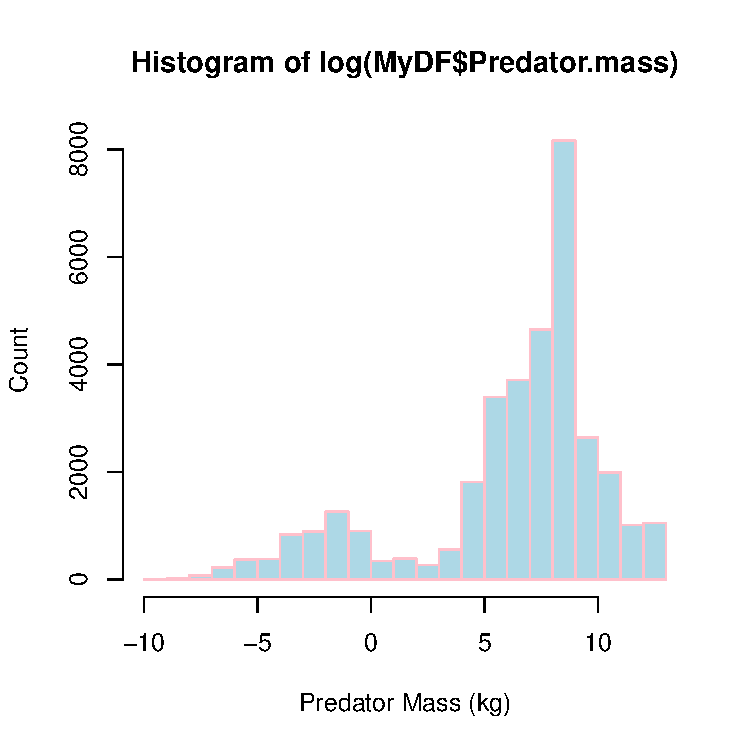
\includegraphics[width=0.5\textwidth]{PrHist3.pdf} 
\end{center}

So, taking a log really makes clearer what the distribution of body 
predator sizes looks like. {\it Try the same with prey body masses.}

\subsubsection{Exercise}

We can do a lot of beautification and fine-tuning of your R plots! As 
an exercise, try adjusting the histogram bin widths to make them same 
for the predator and prey, and making the x and y labels larger and in 
boldface. To get started, look at the help documentation of {\tt hist}.

\subsection{Subplots}
We can also plot both predator and prey body masses in different 
sub-plots using {\tt par} so that we can compare them visually. 

\begin{lstlisting}
> par(mfcol=c(2,1)) #initialize multi-paneled plot
> par(mfg = c(1,1)) # specify which sub-plot to use first 
> hist(log(MyDF$Predator.mass),
    xlab = "Predator Mass (kg)", ylab = "Count", 
    col = "lightblue", border = "pink", 
    main = 'Predator') # Add title
> par(mfg = c(2,1)) # Second sub-plot
> hist(log(MyDF$Prey.mass),
    xlab="Prey Mass (kg)",ylab="Count", 
    col = "lightgreen", border = "pink", 
    main = 'prey')
\end{lstlisting}
\begin{center}
   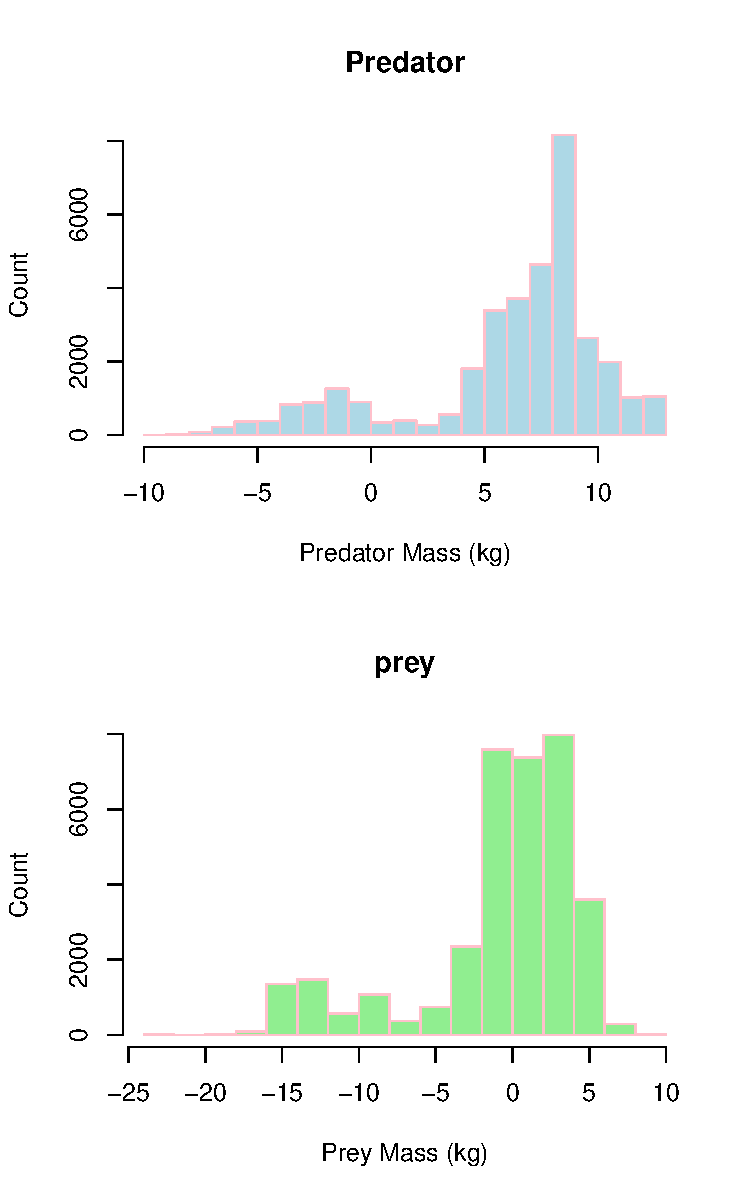
\includegraphics[width=0.5\textwidth]{PPHist1.pdf} 
\end{center}

Another option for making multi-panel plots is the {\tt layout} 
function. 

\subsection{Overlaying plots}
Better still, we would like to see if the predator mass and prey mass 
distributions are similar by overlaying them. 

\begin{lstlisting}
> hist(log(MyDF$Predator.mass), # Predator histogram
    xlab="Body Mass (kg)", ylab="Count", 
    col = rgb(1, 0, 0, 0.5), # Note 'rgb', fourth value is transparency
    main = "Predator-prey size Overlap") 
> hist(log(MyDF$Prey.mass), col = rgb(0, 0, 1, 0.5), add = T) # Plot prey
> legend('topleft',c('Predators','Prey'),   # Add legend
    fill=c(rgb(1, 0, 0, 0.5), rgb(0, 0, 1, 0.5))) # Define legend colors
\end{lstlisting}

\begin{tipbox}
	Plot annotation with text can be done with either single or double 
	quotes, i.e., `Plot Title' or ``Plot Title'', respectively. But it is generally a 
	good idea to use double quotes because sometimes you would like to 
	use an apostrophe in your title or axis label strings.   
\end{tipbox}

\begin{center}
   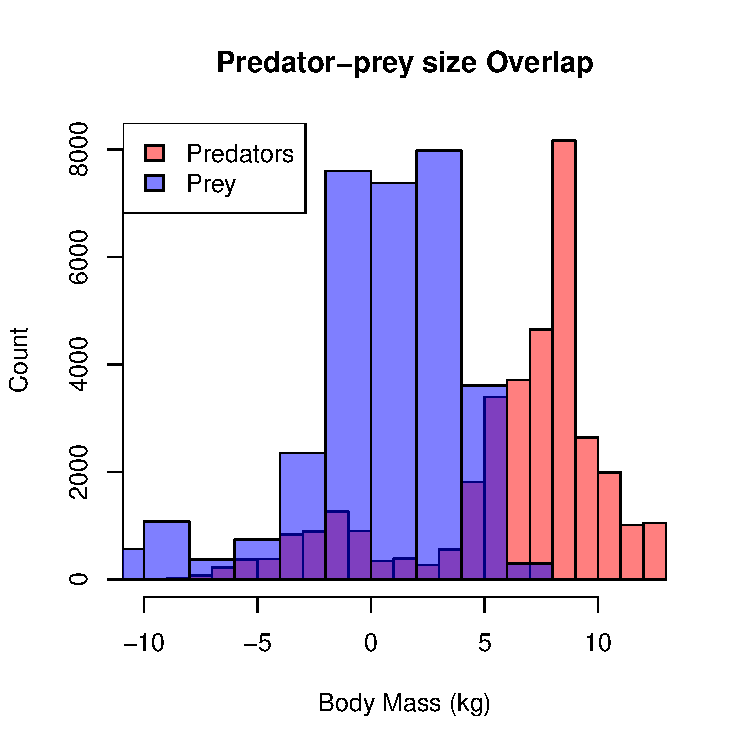
\includegraphics[width=0.5\textwidth]{PPOverlay.pdf} 
\end{center}

{\it It would be nicer to have both the plots with the same bin sizes 
-- try to do it}

\subsection{Boxplots}
Now, let's try plotting boxplots instead of  histograms. These are 
useful for getting a visual summary of the distribution of your data. 

\begin{lstlisting}
> boxplot(log(MyDF$Predator.mass),
	xlab = "Location", ylab = "Predator Mass",
	main = "Predator mass")
\end{lstlisting}
\begin{center}
   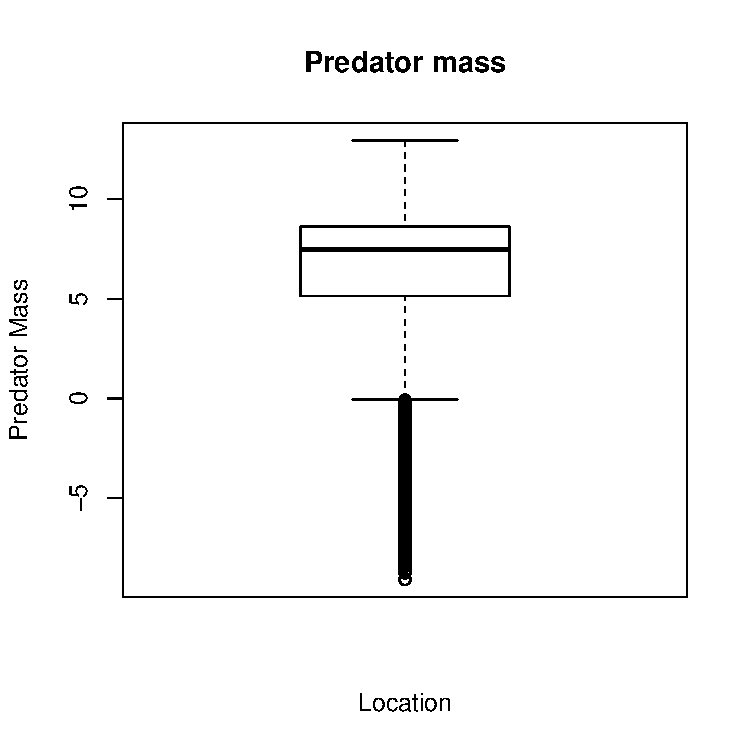
\includegraphics[width=0.5\textwidth]{PredBoxP1.pdf} 
\end{center}

Now let's see how many locations the data are from: 
\begin{lstlisting}
> boxplot(log(MyDF$Predator.mass) ~ MyDF$Location, # Why the tilde?
	xlab = "Location", ylab = "Predator Mass",
	main = "Predator mass by location")
\end{lstlisting}
\begin{center}
   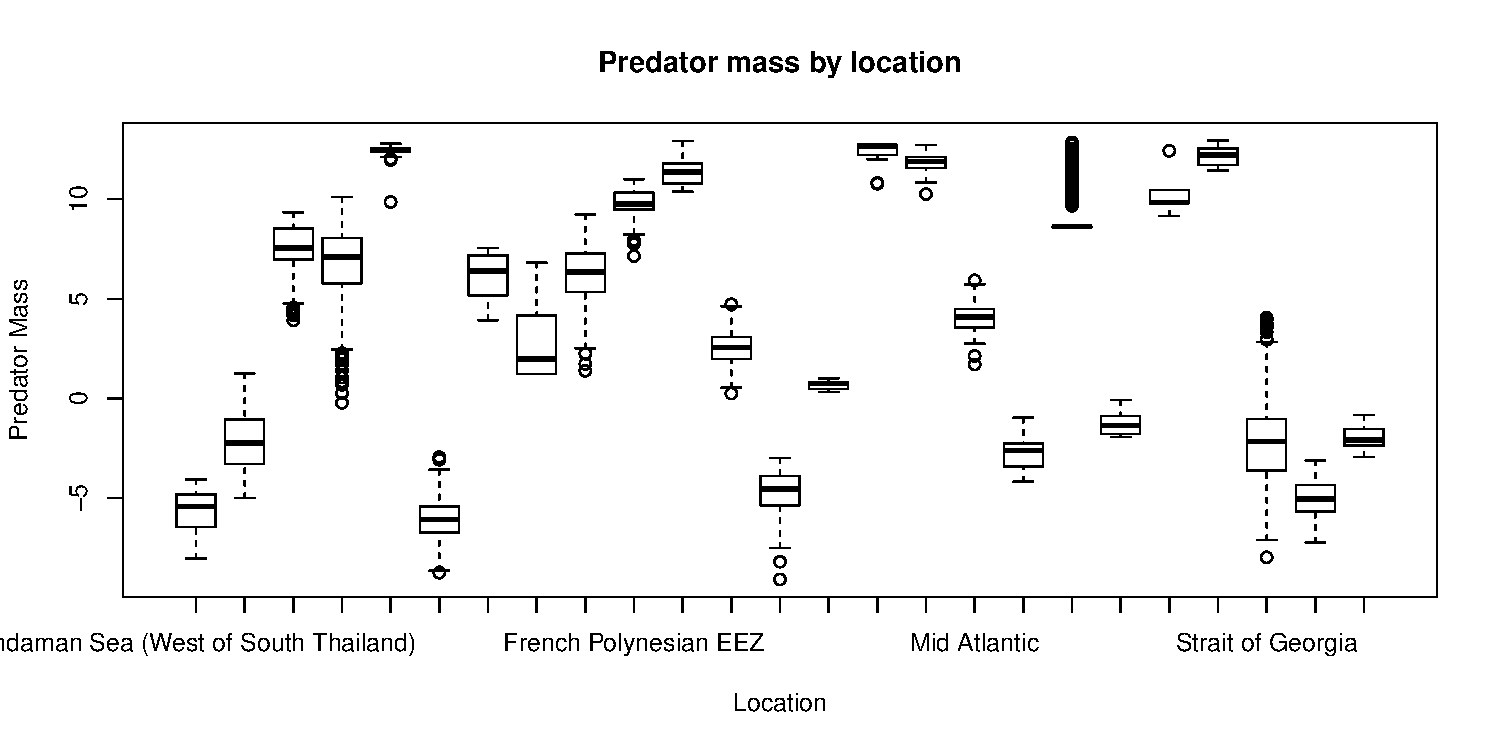
\includegraphics[width=1\textwidth]{PredBoxP2.pdf} 
\end{center}

Note the tilde (\textasciitilde). This is to tell R to subdivide or 
categorize your analysis and plot by the "Factor" location. More on 
this later. 

That's a lot of locations! You will need an appropriately wide plot to 
see all the boxplots adequately. Now let's try boxplots by feeding 
interaction type: 
\begin{lstlisting}
> boxplot(log(MyDF$Predator.mass) ~ MyDF$Type.of.feeding.interaction,
	xlab = "Location", ylab = "Predator Mass",
	main = "Predator mass by feeding interaction type")
\end{lstlisting}

\subsection{Combining plot types}

It would be nice to see both the predator and prey marginal 
distributions as well as the scatterplot for an exploratory analysis. 
We can do this by adding boxplots of the marginal variables to the scatterplot. 

\begin{lstlisting}
> par(fig=c(0,0.8,0,0.8)) # specify figure size as proportion
> plot(log(MyDF$Predator.mass),log(MyDF$Prey.mass),
    xlab = "Predator Mass (kg)", ylab = "Prey Mass (kg)") # Add labels
> par(fig=c(0,0.8,0.55,1), new=TRUE)
> boxplot(log(MyDF$Predator.mass), horizontal=TRUE, axes=FALSE)
> par(fig=c(0.65,1,0,0.8),new=TRUE)
> boxplot(log(MyDF$Prey.mass), axes=FALSE)
> mtext("Fancy Predator-prey scatterplot", side=3, outer=TRUE, line=-3)
\end{lstlisting}

\begin{center}
   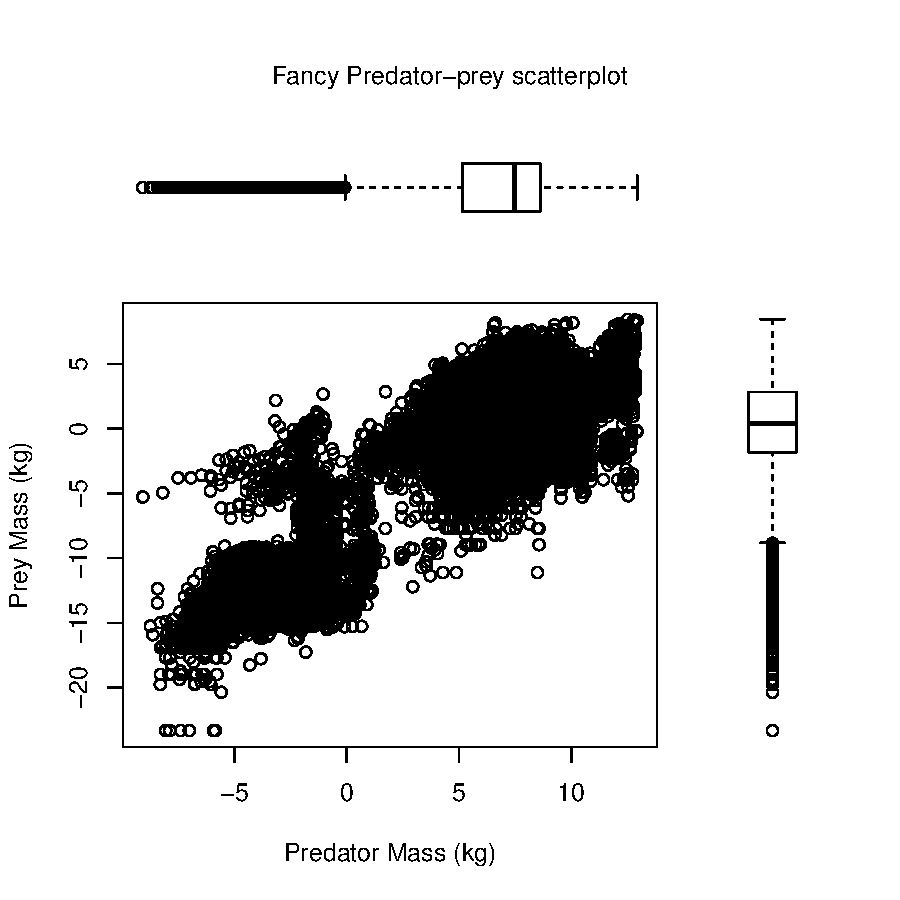
\includegraphics[width=0.6\textwidth]{PPScatFancy.pdf} 
\end{center}
To understand this plotting method, think of the full graph area as 
going from (0,0) in the lower left corner to (1,1) in the upper right 
corner. The format of the {\tt fig=} parameter is a numerical vector of 
the form {\tt c(x1, x2, y1, y2)}. The first {\tt fig= } sets up the 
scatterplot going from 0 to 0.8 on the x axis and 0 to 0.8 on the y 
axis. The top boxplot goes from 0 to 0.8 on the x axis and 0.55 to 1 on 
the y axis. The right hand boxplot goes from 0.65 to 1 on the x axis 
and 0 to 0.8 on the y axis. You can experiment with these proportions 
to change the spacings between plots.

\subsection{Lattice plots}
You can also make lattice graphs to avoid the somewhat laborious {\tt 
par()} approach above of getting multi-panel plots. For this, you will 
need to "load" a "library" that isn't included by default when you run 
R: 

\begin{lstlisting}
> library(lattice)
\end{lstlisting}

\begin{figure}
\centering
	\label{Fig-Lattice-1}
	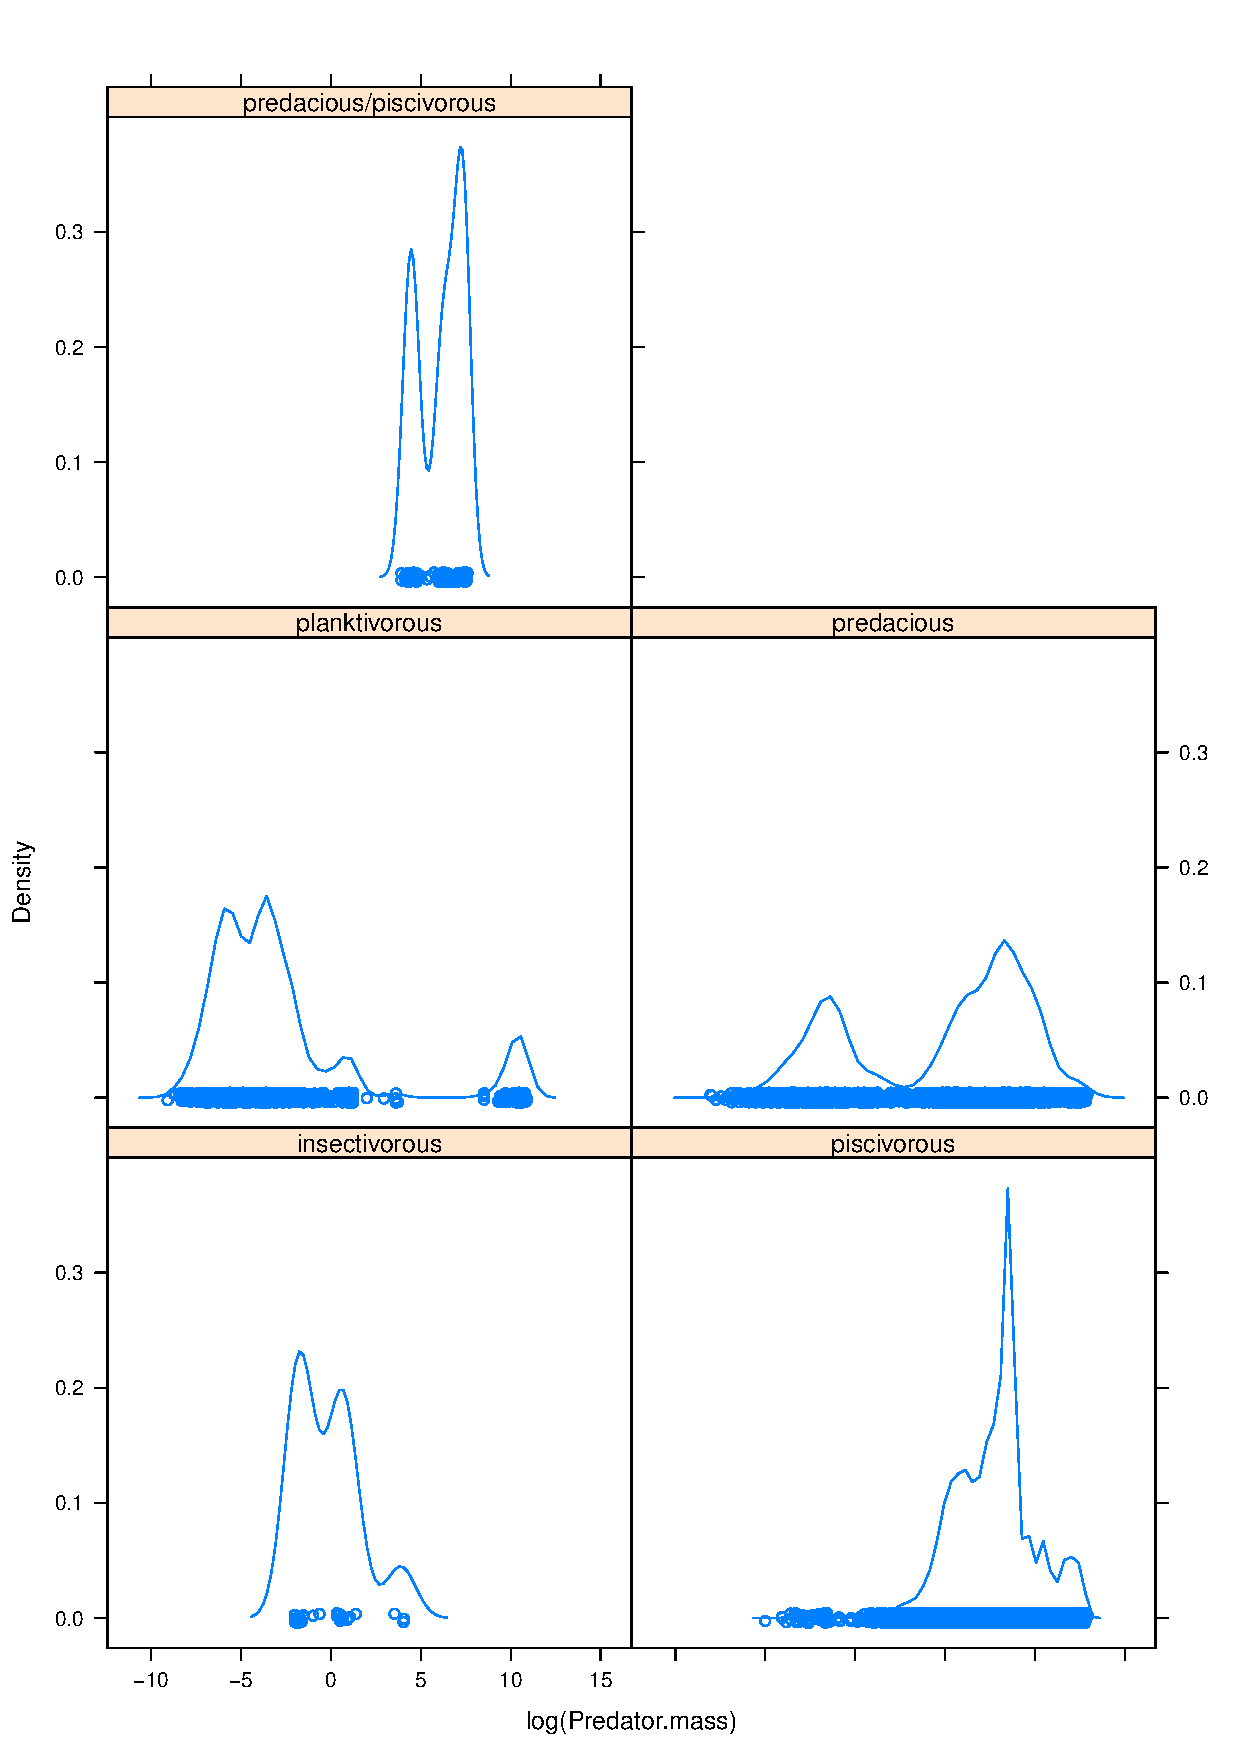
\includegraphics[width = 1 \linewidth]{PP_Lattice.pdf}
	\caption{A {\tt lattice} representation of the predator size data}
\end{figure}

A lattice plot of the above data for predator mass could look like Fig. 
\ref{Fig-Lattice-1} (as a density plot). This was generated using (and 
printing to a pdf with particular dimensions):

\begin{lstlisting}
> densityplot(~log(Predator.mass) | Type.of.feeding.interaction, 
data=MyDF)
\end{lstlisting}

Look up \url{http://www.statmethods.net/advgraphs/trellis.html} and the 
{\tt lattice} package help.

\subsection{Saving your graphics}

And you can also save the figure in a vector graphics format like a 
pdf. It is important to learn to do this, because you want to be able 
to save your plots in good resolution, and want to avoid the manual 
steps of clicking on the figure, doing "save as", etc. So let's 
save the figure as a PDF:  
\begin{lstlisting}
> pdf("../Results/Pred_Prey_Overlay.pdf", # Open blank pdf page 
    11.7, 8.3) # These numbers are page dimensions in inches
> hist(log(MyDF$Predator.mass), # Plot predator histogram (note 'rgb')
    xlab="Body Mass (kg)", ylab="Count", 
    col = rgb(1, 0, 0, 0.5), 
    main = "Predator-Prey Size Overlap") 
> hist(log(MyDF$Prey.mass), # Plot prey weights
    col = rgb(0, 0, 1, 0.5), 
    add = T)  # Add to same plot = TRUE
> legend('topleft',c('Predators','Prey'), # Add legend
    fill=c(rgb(1, 0, 0, 0.5), rgb(0, 0, 1, 0.5))) 
> dev.off() 
\end{lstlisting}

\begin{tipbox}
	Always try to save results in a vector format, which can be scaled up 
	to any size. For more on vector vs raster images/graphics, see: 
	\url{https://en.wikipedia.org/wiki/Vector_graphics}.
\end{tipbox}
Note that you are saving to the {\tt Results} directory now. This 
should always be your workflow: store and retrieve data from a {\tt 
Data} directory, keep your code and work from a {\tt Code} directory, 
and save outputs to a {\tt Results} directory.

You can also try other graphic output formats. For example, {\tt png()} 
(a raster format) instead of {\tt pdf()}. As always, look at the help 
documentation of each of these commands! 

\section{Practicals}
In this practical, you will write script that draws and saves three 
lattice graphs by feeding interaction type: one of predator mass, one 
of prey mass and one of the size ratio of prey mass over predator mass. 
Note that you would want to use logarithms of masses (or mass-ratios) 
for all three plots. In addition, the script will calculate the mean 
and median predator mass, prey mass and predator-prey size-ratios to a 
csv file. So:

\begin{compactitem}[$\quad\star$]
	
	\item Write a script file called {\tt PP\_Lattice.R} and save it in 
	the {\tt Code} directory --- sourcing or running this script should 
	result in three files called {\tt Pred\_Lattice.pdf}, {\tt 
	Prey\_Lattice.pdf}, and {\tt SizeRatio\_Lattice.pdf} being saved in 
	the {\tt Results} directory (the names are self-explanatory, I 
	hope).
    
	\item In addition, the script should calculate the mean and median 
	log predator mass, prey mass, and predator-prey size ratio, {\it by 
	feeding type}, and save it as a single csv output table called	{\tt 
	PP\_Results.csv} to the {\tt Results} directory. The table should 
	have appropriate headers (e.g., Feeding type, mean, median). (Hint: 
	you will have to initialize a new dataframe in the script to first 
	store the calculations) 

	\item The script should be self-sufficient and not need any 
	external inputs --- it should import the above predator-prey 
	dataset from the appropriate directory, and save the graphic plots 
	to the appropriate directory (Hint: use relative paths!).
	
	\item There are multiple ways to do this practical. The plotting and 
	saving component is simple enough. For calculating the statistics by 
	feeding type, you can either use the "loopy" way --- first obtaining 
	a list of feeding types (look up the {\tt unique} or {\tt levels} 
	functions) and then loop over them, using {\tt subset} to extract the 
	dataset by feeding type at each iteration, or the R-savvy way, by 
	using {\tt tapply} or {\tt ddply} and avoiding looping altogether 
	(Chapter \ref{chap:R_II}).
	
\end{compactitem}

%%%%%%%%%%%%%%%%%%%%%%%%%%%%%%%%%%%%%%%%%%%%%%%%%%%%%%%%%%%%%%%%%%%
%%%%%%%%%%%%%%%%%%%%%%%%%%%%%%%%%%%%%%%%%%%%%%%%%%%%%%%%%%%%%%%%%%%

\section{Publication-quality figures in R}

{\tt R} can produce beautiful graphics, but it takes a lot of work to 
obtain the desired result. This is because the starting point is pretty 
much a ``bare'' plot, and adding features commonly required for 
publication-grade figures (legends, statistics, regressions, etc.) can 
be quite involved. 
	
Moreover, it is very difficult to switch from one representation of the 
data to another (i.e., from boxplots to scatterplots), or to plot 
several datasets together. The {\tt R} package {\tt ggplot2} overcomes 
these issues, and produces truly high-quality, publication-ready 
graphics suitable for papers, theses and reports. 

\begin{tipbox}
Currently, {\tt ggplot2} cannot be used to create 3D graphs or mosaic 
plots. In any case, most of you won't be needing 3D plots! If you do, 
there are many ways to do 3D plots using other plotting packages in R. 
In particular, look up the {\tt scatterplot3d} and {\tt plot3D} 
packages.
\end{tipbox}

% \section{Fundamental rules of visualization}

% \begin{compactitem}

	% \item Make sure the text within the figure and outside on the axes ad 
	% labels will be visible at about once you rescale the figure to its 
	% final size. 
	
	% \item Be careful about reds and greens --- as many as 10\% of men can 
	% be color-blind!
	
	% \item Use vector, not raster graphics (to the extent possible)
	
% \end{compactitem}

{\tt ggplot2} differs from other approaches as it attempts to provide a 
``grammar'' for graphics in which each layer is the equivalent of a 
verb, subject etc. and a plot is the equivalent of a sentence. All 
graphs start with a layer showing the data, other layers and commands 
are added to modify the plot. Specifically, according to this grammar, 
a statistical graphic is a ``mapping'' from data to aesthetic 
attributes (colour, shape, size; set using {\tt aes}) of geometric 
objects (points, lines, bars; set using {\tt geom}).  

For more on the ideas underlying ggplot, see the book ``ggplot2: 
Elegant Graphics for Data Analysis'', by H. Wickham (in your Reading 
directory). Also, the website \url{ ggplot2.org} a great resource. 

{\tt ggplot2} should already be available on the college computers. If 
you are using your own computer, look up the section on installing 
packages in Chapter \ref{chap:RI}. 

ggplot can be used in two ways: with {\tt qplot} (for {\tt q}uick {\tt 
plot}ting) and {\tt ggplot} for full-blown, customizable plotting.

\begin{tipbox}
Note that {\tt ggplot2} only accepts data in data frames. 	
\end{tipbox}

\subsection{Basic plotting with {\tt qplot}}

{\tt qplot} can be used to quickly produce graphics for exploratory 
data analysis, and as a base for more complex graphics. It uses syntax 
that is closer to the standard R plotting commands. 

We will use the same predator-prey body size dataset again -- you will 
soon see how much nice the same types of plots you made above look when 
done with ggplot!. 

\subsubsection{Scatterplots}

Let's start plotting the {\tt Predator.mass} vs {\tt Prey.mass}:
\begin{lstlisting}
> require(ggplot2)  ## Load the package
Loading required package: ggplot2
> qplot(Prey.mass, Predator.mass, data = MyDF)
\end{lstlisting}

As before, let's take logarithms and plot:

\begin{lstlisting}
> qplot(log(Prey.mass), log(Predator.mass), data = MyDF)
\end{lstlisting}

Now, color the points according to the type of feeding interaction:

\begin{lstlisting}
> qplot(log(Prey.mass), log(Predator.mass), data = MyDF, 
	colour = Type.of.feeding.interaction)
\end{lstlisting}

The same as above, but changing the shape:
\begin{lstlisting}
> qplot(log(Prey.mass), log(Predator.mass), data = MyDF, 
	shape = Type.of.feeding.interaction)
\end{lstlisting}

\subsubsection{Aesthetic mappings}
These examples demonstrate a key difference between {\tt qplot} and the 
standard {\tt plot} command: When you want to assign colours, sizes or 
shapes to the points on your plot, using the {\tt plot} command, it's 
your responsibility to convert (i.e., ``map'') a categorical variable 
in your data (e.g., type of feeding interaction in the above case) onto 
colors (or shapes) that {\tt plot} knows how to use (e.g., by 
specifying ``red'', ``blue'', ``green'', etc). 

ggplot does this mapping for you automatically, and also provides a 
legend! This makes it really easy to quickly include additional data 
(e.g., if a new feeding interaction type was added to the data) on the 
plot. 

Instead of using ggplot's automatic mapping, if you want to  manually 
set a color or a shape, you have to use {\tt I()} (meaning 
``Identity''). To see this in practice, try the following:
\begin{lstlisting}
> qplot(log(Prey.mass), log(Predator.mass), 
	data = MyDF, colour = "red")
\end{lstlisting}
You chose red, but ggplot used mapping to convert it to a particular 
shade of red. To set it manually to the real red, do this:
\begin{lstlisting}
> qplot(log(Prey.mass), log(Predator.mass), 
	data = MyDF, colour = I("red"))
\end{lstlisting}

Similarly, for point size, compare these two:
\begin{lstlisting}
> qplot(log(Prey.mass), log(Predator.mass), 
	data = MyDF, size = 3) #with ggplot size mapping
> qplot(log(Prey.mass), log(Predator.mass), 
	data = MyDF, size = I(3)) #no mapping
\end{lstlisting}

But for shape, ggplot doesn't have a continuous mapping because shapes 
are a discrete variable. To see this, compare these two:
\begin{lstlisting}
> qplot(log(Prey.mass), log(Predator.mass), 
	data = MyDF, shape = 3) #will give error
> qplot(log(Prey.mass), log(Predator.mass), 
	data = MyDF, shape= I(3))
\end{lstlisting}

\subsubsection{Setting transparency}
Because there are so many points, we can make them semi-transparent 
using {\tt alpha} so that the overlaps can be seen:
\begin{lstlisting}
> qplot(log(Prey.mass), log(Predator.mass), data = MyDF, 
	colour = Type.of.feeding.interaction, alpha = I(.5))
\end{lstlisting}
Here try using {\tt alpha = .5} instead of {\tt alpha = I(.5)} and see 
what happens.

\subsubsection{Adding smoothers and regression lines}

Now add a smoother to the points: 
\begin{lstlisting}
> qplot(log(Prey.mass), log(Predator.mass), data = MyDF, 
	geom = c("point", "smooth"))
\end{lstlisting}

If we want to have a linear regression, we need to specify the method 
as being {\tt lm}:

\begin{lstlisting}
> qplot(log(Prey.mass), log(Predator.mass), data = MyDF, 
	geom = c("point", "smooth")) + geom_smooth(method = "lm")
\end{lstlisting}

{\tt lm} stands for {\tt l}inear {\tt m}odels (linear regression is a type 
of linear model). You will learn about linear models and fitting them 
to data (as you have done here) in the Stats in R week. 

We can also add a ``smoother'' for each type of interaction:
\begin{lstlisting}
> qplot(log(Prey.mass), log(Predator.mass), data = MyDF, 
	geom = c("point", "smooth"), colour = Type.of.feeding.interaction)  
				+ geom_smooth(method = "lm")
\end{lstlisting}

To extend the lines to the full range, use {\tt fullrange = TRUE}:

\begin{lstlisting}
> qplot(log(Prey.mass), log(Predator.mass), data = MyDF, 
	geom = c("point", "smooth"),
	colour = Type.of.feeding.interaction) + 
	geom_smooth(method = "lm",fullrange = TRUE)
\end{lstlisting}

Now we want to see how the ratio between prey and predator mass changes 
according to the type of interaction:

\begin{lstlisting}
> qplot(Type.of.feeding.interaction, 
		log(Prey.mass/Predator.mass), data = MyDF)
\end{lstlisting}

Because there are so many points, we can ``jitter'' them to get a
better idea of the spread:

\begin{lstlisting}
> qplot(Type.of.feeding.interaction, 
		log(Prey.mass/Predator.mass), data = MyDF,
		geom = "jitter")
\end{lstlisting}

\subsubsection{Boxplots}

Or we can draw a boxplot of the data (note the {\tt geom} argument, 
which stands for {\tt geom}etry):

\begin{lstlisting}
> qplot(Type.of.feeding.interaction, 
		log(Prey.mass/Predator.mass), data = MyDF,
		geom = "boxplot")
\end{lstlisting}

\subsubsection{Histograms and density plots}

Now let's draw an histogram of predator-prey mass ratios:

\begin{lstlisting}
> qplot(log(Prey.mass/Predator.mass), data = MyDF, 
	geom =  "histogram")
\end{lstlisting}

Color the histogram according to the interaction type:

\begin{lstlisting}
> qplot(log(Prey.mass/Predator.mass), data = MyDF, 
	geom =  "histogram", 
	fill = Type.of.feeding.interaction)
\end{lstlisting}

You may want to define binwidth (in units of x axis):

\begin{lstlisting}
> qplot(log(Prey.mass/Predator.mass), data = MyDF, 
	geom =  "histogram", 
	fill = Type.of.feeding.interaction,
	binwidth = 1)
\end{lstlisting}

To make it easier to read, we can plot the smoothed density of the 
data:

\begin{lstlisting}
> qplot(log(Prey.mass/Predator.mass), data = MyDF, 
	geom =  "density", fill = Type.of.feeding.interaction)
\end{lstlisting}

And you can make the densities transparent so that the overlaps are 
visible:

\begin{lstlisting}
> qplot(log(Prey.mass/Predator.mass), data = MyDF, 
	geom =  "density", fill = Type.of.feeding.interaction, alpha = 
	I(0.5))
\end{lstlisting}

Or using {\tt colour} instead of {\tt fill} draws only the edge of
the curve:
\begin{lstlisting}
> qplot(log(Prey.mass/Predator.mass), data = MyDF, 
	geom =  "density", colour = Type.of.feeding.interaction)
\end{lstlisting}

Similarly, {\tt geom = "bar"} produces a barplot, {\tt geom =
	"line"} a series of points joined by a line, etc.

\subsubsection{Multi-faceted plots}
An alternative way of displaying data belonging to different classes
is using ``faceting''. We did this using {\tt 
lattice()} previously, but ggplot does a much nicer job:

\begin{lstlisting}
> qplot(log(Prey.mass/Predator.mass), 
	facets = Type.of.feeding.interaction ~., 
	data = MyDF, geom =  "density")
\end{lstlisting}

The {\tt \textasciitilde .} (the space is not important) notation tells 
ggplot whether to do the faceting by row or by column. So if you want a 
by-column configuration, switch {\tt \textasciitilde} and {\tt .}, and 
also swap the position of the {\tt .\textasciitilde}:

\begin{lstlisting}
> qplot(log(Prey.mass/Predator.mass), 
	facets =  .~ Type.of.feeding.interaction, 
	data = MyDF, geom =  "density")
\end{lstlisting}

You can also facet by a combination of categories (this is going to be 
a big plot!):

\begin{lstlisting}
> qplot(log(Prey.mass/Predator.mass), 
	facets = .~ Type.of.feeding.interaction + Location, 
	data = MyDF, geom =  "density")
\end{lstlisting}

And you can also change the order of the combination:

\begin{lstlisting}
> qplot(log(Prey.mass/Predator.mass), 
	facets = .~ Location + Type.of.feeding.interaction, 
	data = MyDF, geom =  "density")
\end{lstlisting}

\begin{tipbox}
	For more fine-tuned faceting, look up the {\tt facet\_grid()} and 
	{\tt facet\_wrap()} functions within {\tt ggplot2}. look up \url{ 
	http://www.cookbook-r.com/Graphs/Facets_(ggplot2)}. 
	
	See Fig. \ref{PPRegress} for an example result. 
\end{tipbox}

\subsubsection{Logarithmic axes}
A more elegant way of drawing logarithmic quantities is to set the axes 
to be logarithmic:

\begin{lstlisting}
> qplot(Prey.mass, Predator.mass, data = MyDF, log="xy")
\end{lstlisting}

\subsubsection{Plot annotations}

Let's add a title and labels:

\begin{lstlisting}
> qplot(Prey.mass, Predator.mass, data = MyDF, log="xy",
	main = "Relation between predator and prey mass", 
	xlab = "log(Prey mass) (g)", 
	ylab = "log(Predator mass) (g)")
\end{lstlisting}

Adding {\tt + theme\_bw()} makes it suitable for black and white
printing.

\begin{lstlisting}
> qplot(Prey.mass, Predator.mass, data = MyDF, log="xy",
	main = "Relation between predator and prey mass", 
	xlab = "Prey mass (g)", 
	ylab = "Predator mass (g)") + theme_bw()
\end{lstlisting}

\subsubsection{Saving your plots}

Finally, let's save a pdf file of the figure (same approach as we used 
before):
\begin{lstlisting}
> pdf("../Results/MyFirst-ggplot2-Figure.pdf")
> print(qplot(Prey.mass, Predator.mass, data = MyDF,log="xy",
	main = "Relation between predator and prey mass", 
	xlab = "log(Prey mass) (g)", 
	ylab = "log(Predator mass) (g)") + theme_bw())
> dev.off()
\end{lstlisting}

Using {\tt print} ensures that the whole command is kept together and 
that you can use the command in a script.

\subsection{Some more important ggplot options}
Other important options to keep in mind:

\begin{tabular}{p{1.8cm} p{11cm}} 
	{\tt xlim} & limits for x axis: {\tt xlim = c(0,12)}\\
	{\tt ylim} & limits for y axis\\
	{\tt log} & log transform variable {\tt log = "x"},
		{\tt log = "y"}, {\tt log = "xy"}\\
	{\tt main} & title of the plot {\tt main = "My Graph"}\\
	{\tt xlab} & x-axis label\\
	{\tt ylab} & y-axis label\\
	{\tt asp} & aspect ratio  {\tt asp = 2}, {\tt asp = 0.5}\\
	{\tt margins} & whether or not margins will be displayed\\
\end{tabular}\\

\subsection{Various {\tt geom}}

{\tt geom} Specifies the geometric objects that define the graph type. 
The geom option is expressed as a character vector with one or more 
entries. geom values include "point", "smooth", "boxplot", "line", 
"histogram", "density", "bar", and "jitter". Try the following:

\lstinputlisting[language=R]{Practicals/Code/qplotExamples.R}

\subsection{Advanced plotting: {\tt ggplot}}

The command {\tt qplot} allows you to use only a single dataset and
a single set of ``aesthetics'' (x, y, etc.). To make full use of
{\tt ggplot2}, we need to use the command {\tt ggplot}, which allows 
you to use ``layering''. Layering is the mechanism by which additional 
data elements are added to a plot. Each layer can come from a different 
dataset and have a different aesthetic mapping, allowing us to create 
plots that could not be generated using {\tt qplot()}, which permits 
only a single dataset and a single set of aesthetic mappings. 

For a {\tt ggplot} plotting command, we need at least:
\begin{itemize}
	\item The data to be plotted, in a data frame;
	\item Aesthetics mappings, specifying which variables we want to
	plot, and how;
	\item The {\tt geom}, defining the geometry for representing the data;
	\item (Optionally) some {\tt stat} that transforms the data or
	performs statistics using the data.
\end{itemize}

To start a graph, we nust specify the data and the aesthetics:

\begin{lstlisting}
> p <- ggplot(MyDF, aes(x = log(Predator.mass),
				y = log(Prey.mass),
				colour = Type.of.feeding.interaction ))
\end{lstlisting}

Here we have created a graphics object {\tt p} to which we can add 
layers and other plot elements. 

Now try to plot the graph:

\begin{lstlisting}
> p
Error: No layers in plot
\end{lstlisting}

That is because we are yet to specify a geometry --- only then can we 
see the graph:

\begin{lstlisting}
> p + geom_point()
\end{lstlisting}

We can use the ``plus'' sign to concatenate different commands:

\begin{lstlisting}
> p <- ggplot(MyDF, aes(x = log(Predator.mass),
				y = log(Prey.mass),
				colour = Type.of.feeding.interaction ))
> q <- p + geom_point(size=I(2), shape=I(10)) + theme_bw()
> q
\end{lstlisting}

Let's remove the legend:

\begin{lstlisting}
> q + theme(legend.position = "none")
\end{lstlisting}

We will not look at some case studies to see some useful ways in which
you can use ggplot.

\subsection{Case study 1: plotting a matrix}
\begin{figure}
	\begin{center}
	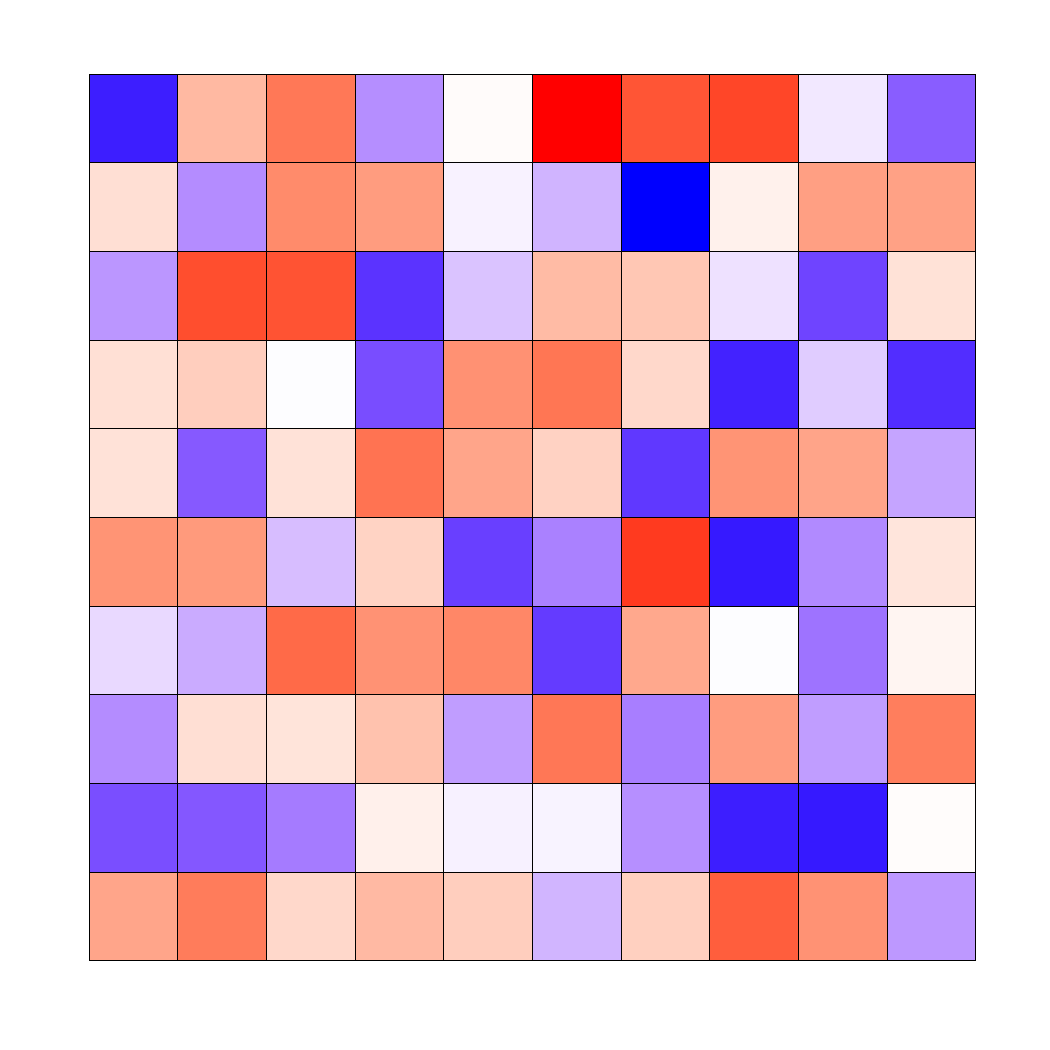
\includegraphics[width = 0.5 \linewidth]{FigureMatrix.pdf}
	\end{center}
	\caption{Random matrix with values sampled from uniform
	distribution.}
	\label{MatPlot}
\end{figure}

Here we will plot a matrix of random values taken from a normal 
distribution $\mathcal U [0,1]$. Our goal is to produce the plot in 
Figure \ref{MatPlot}. Because we want to plot a matrix, and {\tt 
ggplot2} accepts only dataframes, we use the package {\tt reshape2} 
that can ``melt'' a matrix into a dataframe:

\begin{lstlisting}
require(ggplot2)
require(reshape2)

GenerateMatrix <- function(N){
	M <- matrix(runif(N * N), N, N)
	return(M)
}

> M <- GenerateMatrix(10)

> M[1:3, 1:3]
			[,1]      [,2]      [,3]
[1,] 0.2700254 0.8686728 0.7365857
[2,] 0.1744879 0.8488169 0.4165879
[3,] 0.3980783 0.7727821 0.4271121

> Melt <- melt(M)

> Melt[1:4,]
  Var1 Var2     value
1    1    1 0.0698925
2    2    1 0.6333296
3    3    1 0.8990120
4    4    1 0.8425578

> ggplot(Melt, aes(Var1, Var2, fill = value)) + geom_tile()

# adding a black line dividing cells
> p <- ggplot(Melt, aes(Var1, Var2, fill = value))
> p <- p + geom_tile(colour = "black")

# removing the legend
> q <- p + theme(legend.position = "none")

# removing all the rest
> q <- p + theme(legend.position = "none", 
	 panel.background = element_blank(),
	 axis.ticks = element_blank(), 
	 panel.grid.major = element_blank(),
	 panel.grid.minor = element_blank(),
	 axis.text.x = element_blank(),
	 axis.title.x = element_blank(),
	 axis.text.y = element_blank(),
	 axis.title.y = element_blank())

# exploring the colors
> q + scale_fill_continuous(low = "yellow",
						high = "darkgreen")
> q + scale_fill_gradient2()
> q + scale_fill_gradientn(colours = grey.colors(10))
> q + scale_fill_gradientn(colours = rainbow(10))
> q + scale_fill_gradientn(colours =
				c("red", "white", "blue"))
\end{lstlisting}

% check if scale_fill_gradient2() is deprecated

\subsection{Case study 2: plotting two dataframes}

According to Girko's circular law, the eigenvalues of a matrix $M$ of
size $N \times N$ are approximately contained in a circle in the
complex plane with radius $\sqrt{N}$. We are going to draw a
simulation displaying this result (Figure \ref{Girko}).

\lstinputlisting[language=R]{Practicals/Code/Eigen.R}
\begin{figure}\centering
	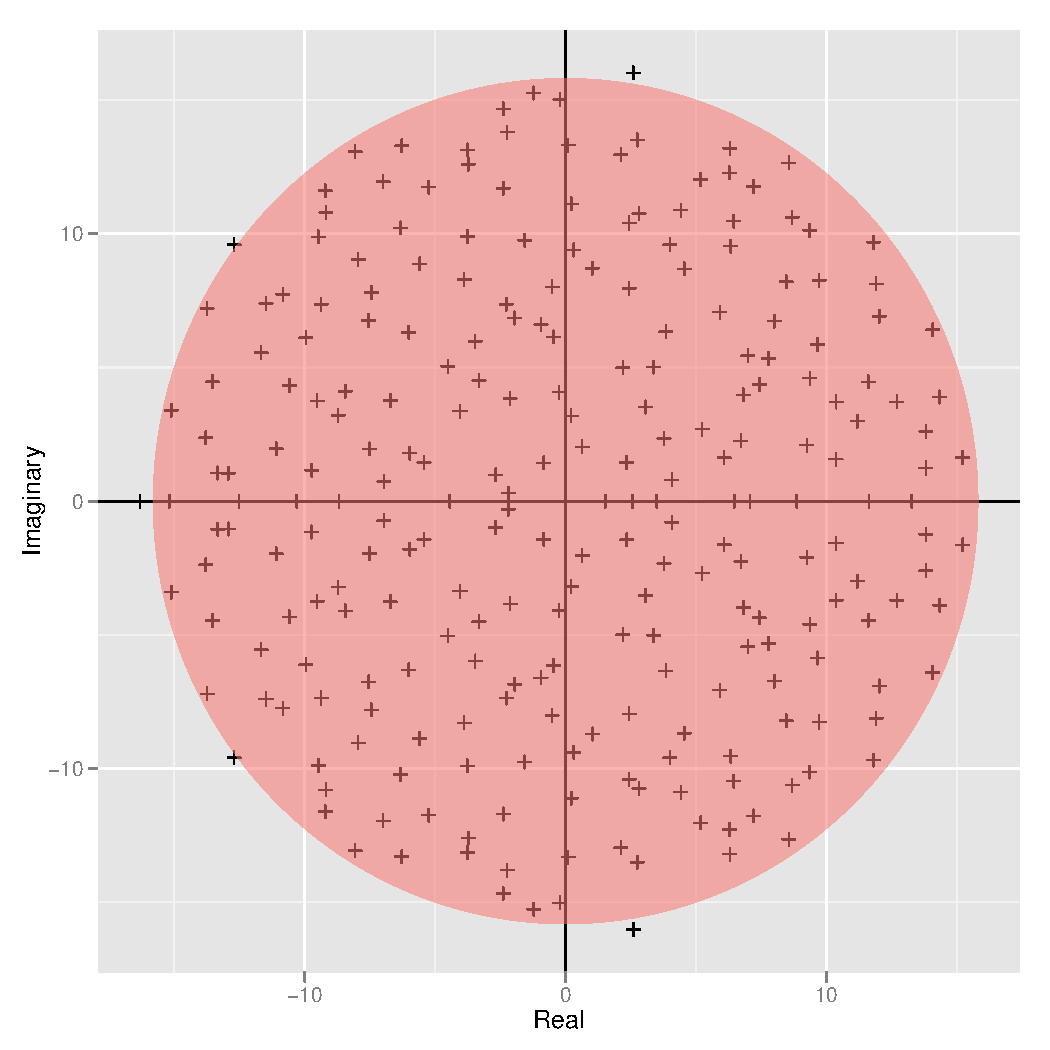
\includegraphics[width = 0.6\linewidth]{Girko.pdf}
	\caption{Girko's circular law.}
	\label{Girko}
\end{figure}

\subsection{Case study 3: annotating plots}

In the plot in Figure \ref{Linebar}, we use the geometry ``text'' to
annotate the plot.

\lstinputlisting[language=R]{Practicals/Code/bars.R}
\begin{figure}
	\begin{center}
	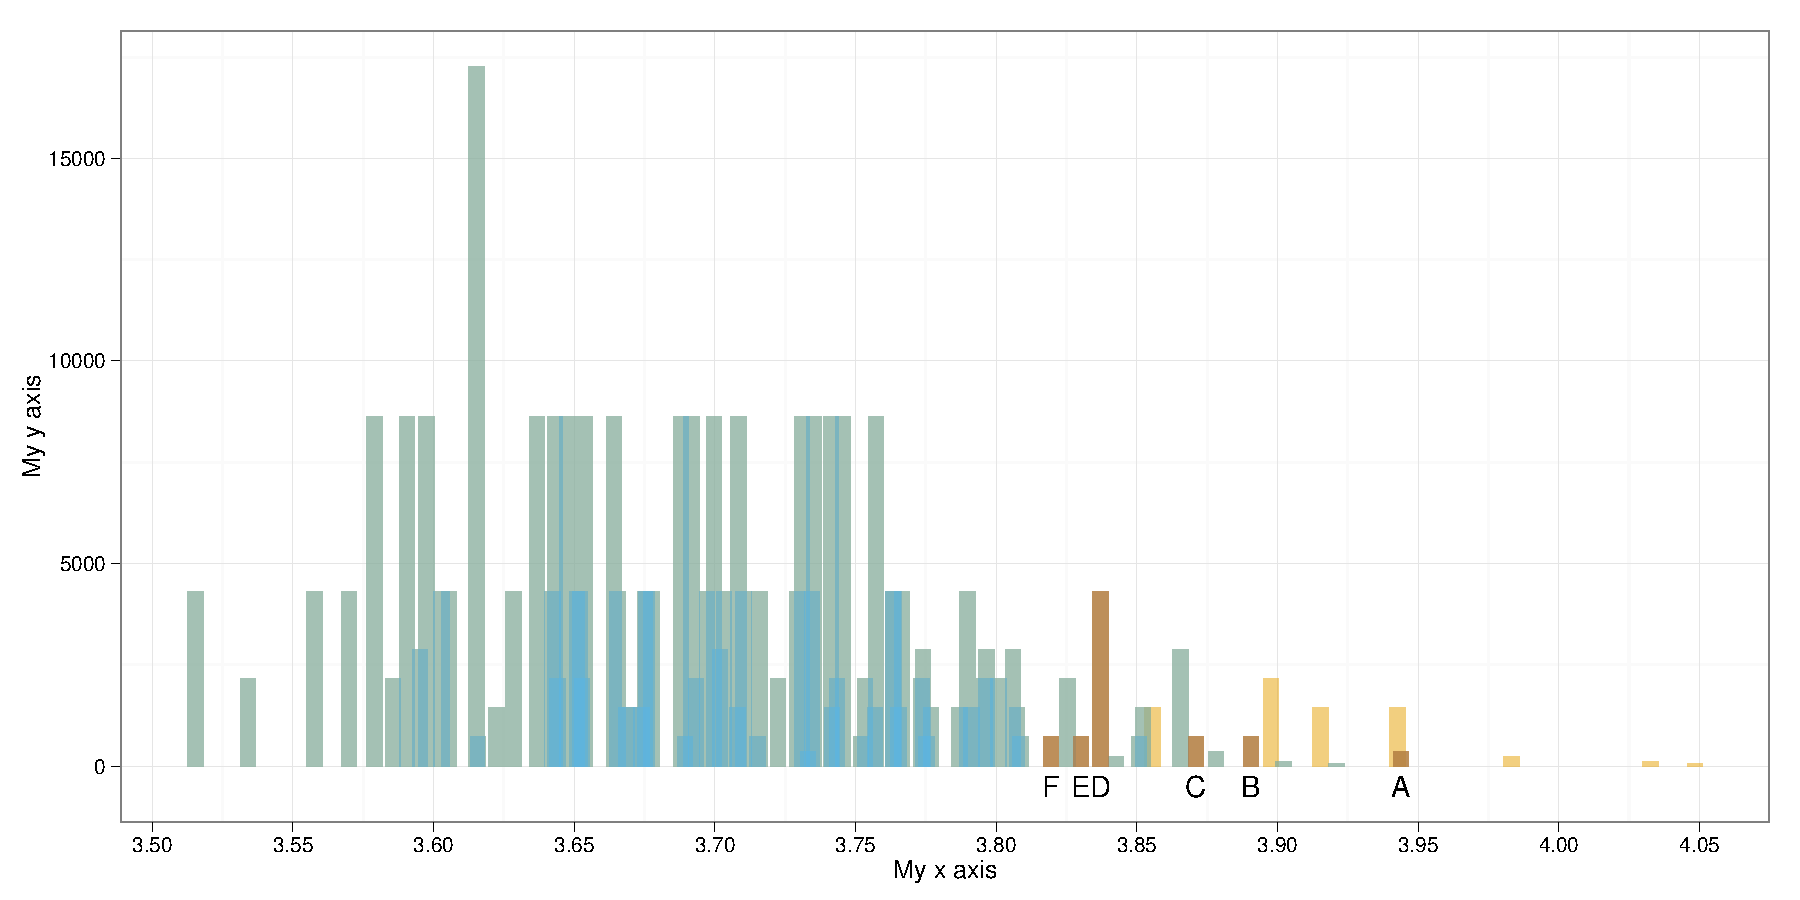
\includegraphics[width = \linewidth]{MyBars.pdf}
	\end{center}
	\caption{Overlay of three lineranges and a text geometry.}
	\label{Linebar}
\end{figure}

\subsection{Case study 4: mathematical display}
\lstinputlisting[language=R]{Practicals/Code/plotLin.R}
\begin{figure}
	\begin{center}
	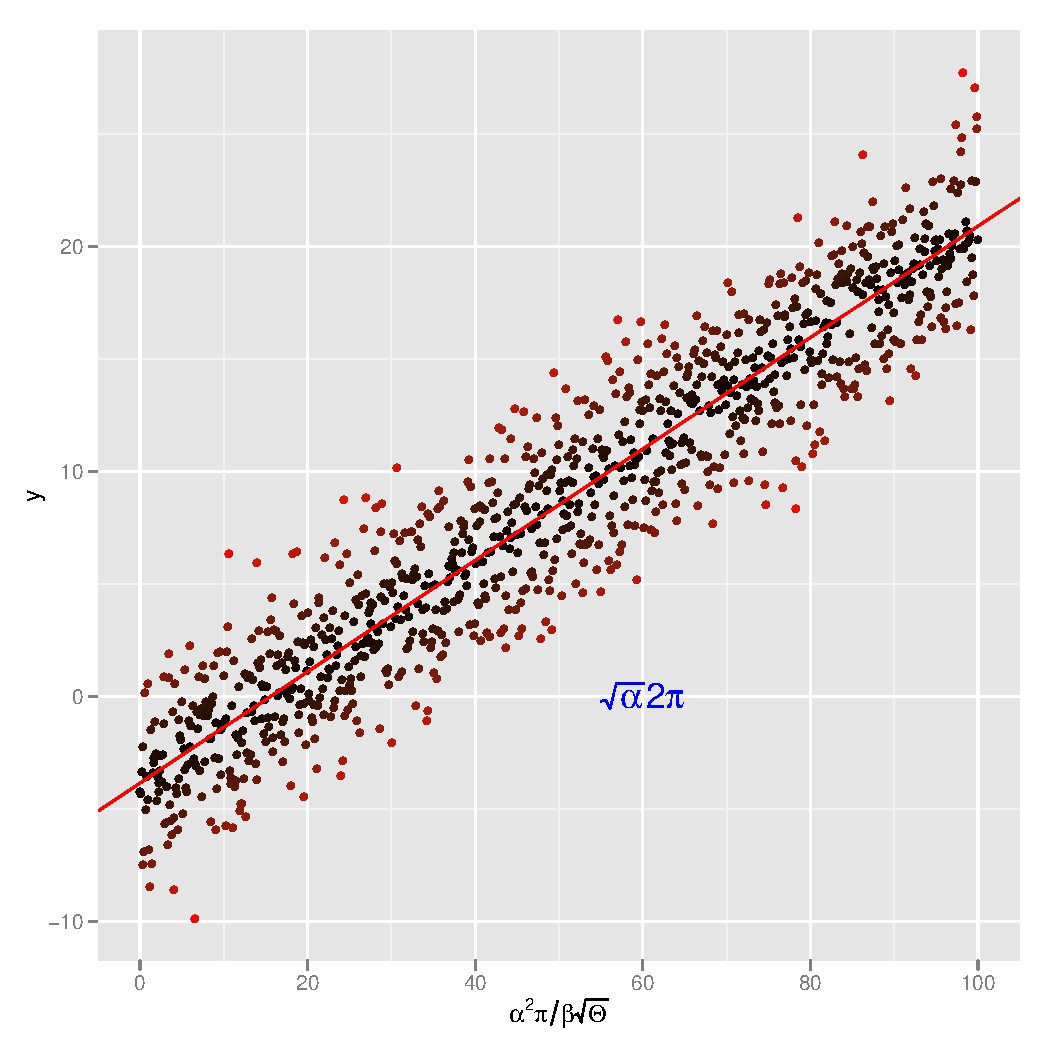
\includegraphics[width = .7\linewidth]{MyLinReg.pdf}
	\end{center}
	\caption{Linear regression with colors expressing residuals and
	mathematical annotations.}
	\label{LinReg}
\end{figure}

In Figure \ref{LinReg}, you can see the mathematical annotation on the
axis and in the plot area itself.

\subsection{\tt ggthemes}

The package {\tt ggthemes} provides you some additional {\tt geom}s, {\tt 
scale}s, and {\tt theme}s for {\tt ggplot}. These include a theme based 
on Tufte's {\it The Visual Display of Quantitative Information} (see 
the readings section at the end of this Chapter). First install the 
package:

\begin{lstlisting}
> install.packages("ggthemes")
\end{lstlisting}

Then try:

\begin{lstlisting}	
> library(ggthemes)

p <- ggplot(MyDF, aes(x = log(Predator.mass), y = log(Prey.mass),
				colour = Type.of.feeding.interaction )) +
				geom_point(size=I(2), shape=I(10)) + theme_bw()

> p + geom_rangeframe() + # now fine tune the geom to Tufte's range frame
		theme_tufte() # and theme to Tufte's minimal ink theme    
\end{lstlisting}

Go to \url{https://github.com/jrnold/ggthemes} for more 
information and a list of {\tt geom}s, {\tt theme}s, and {\tt scale}s. 

\begin{tipbox}
Both {\tt library()} and {\tt require()} are commands/functions to load 
packages. The difference is that {\tt require()} is designed for use 
inside other functions, so it returns {\tt FALSE} and gives a warning, 
whereas {\tt library()} returns an error by default if the package does 
not exist. 
\end{tipbox}

\section{Practicals} \label{sec:PPPrac2}
In this practical, you will write script that draws and saves a pdf 
file of Fig. \ref{PPRegress}, and writes the accompanying 
regression results to a formatted table in csv. Note that the plots 
show that the analysis must be subsetted by the {\tt 
Predator.lifestage} field of the dataset. The guidelines are:

\begin{compactitem}
		
	\item Write a {\tt R} script file called {\tt PP\_Regress.R} and save it in 
	the {\tt Code} directory --- sourcing or running this script should 
	result in one pdf file containing the following figure being 
	saved in the {\tt Results} directory:
	(Hint: Use the {\tt print()} command to write to the pdf)    
\end{compactitem}

\begin{figure}
	\begin{center}
				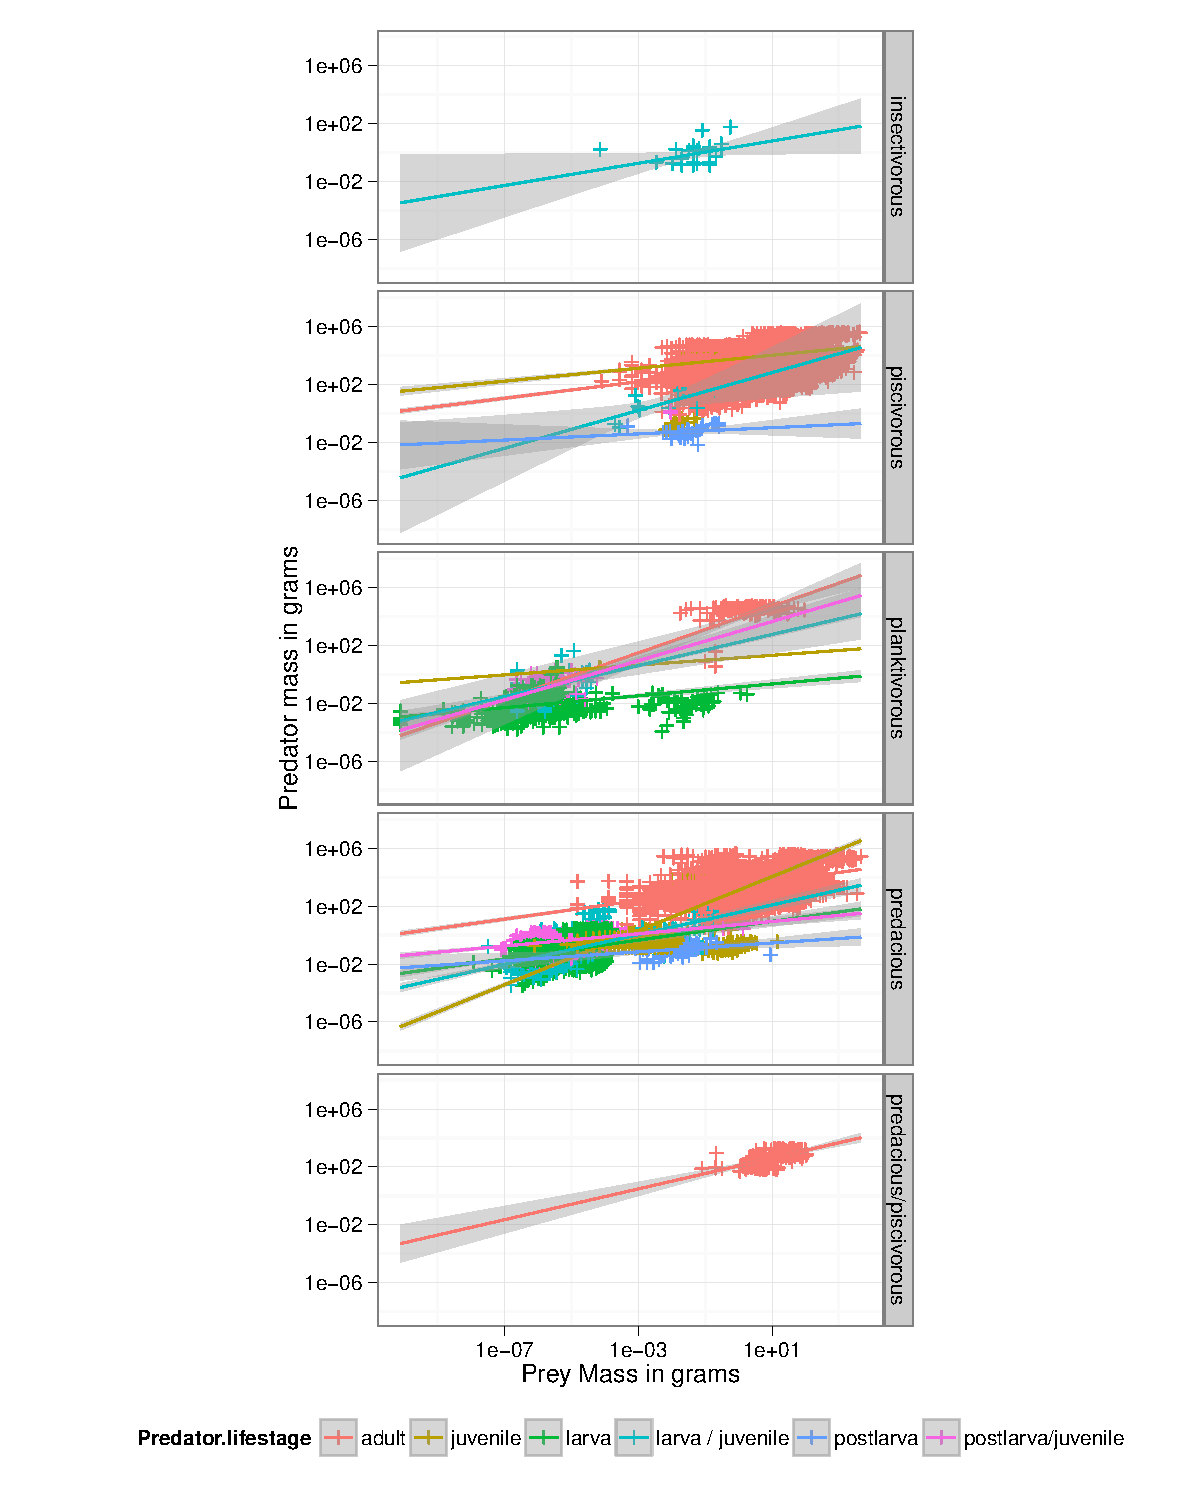
\includegraphics[scale=0.7]{Figure1.pdf}
	\end{center}
	\caption{Write a script that generates this figure}
	\label{PPRegress}
\end{figure}
	
\begin{compactitem}
	\item In addition, the script should calculate the regression results 
	corresponding to the lines fitted in the figure and save it to a csv 
	delimited table called ({\tt PP\_Regress\_Results.csv}), in the {\tt 
	Results} directory. (Hint: you will have to initialize a new 
	dataframe in the script to first store the calculations and then {\tt 
	write.csv()} or {\tt write.table()} it.) \\ 
	All that you are being asked for here is results of an analysis of 
	Linear regression on subsets of the data corresponding to available 
	Feeding Type $\times$ Predator life Stage combination --- not a 
	multivariate linear model with these two as separate covariates!

	\item The regression results should include the following with 
	appropriate headers (e.g., slope, intercept, etc, in each Feeding 
	type $\times$ life stage category): regression slope, regression 
	intercept, R$^2$, F-statistic value, and p-value of the overall 
	regression (Hint: Review the Stats week!).
 
 	\item The script should be self-sufficient and not need any 
	external inputs --- it should import the above predator-prey 
	dataset from the appropriate directory, and save the graphic plots 
	to the appropriate directory (Hint: use relative paths). I should 
	be able to {\tt source} it without errors.

	\item You can also use the {\tt dplyr} function instead of looping 
	(se Chapter \ref{chap:R_II}), and the {\tt ggplot} command 
	instead of {\tt qplot}.

\end{compactitem}

\noindent {\bf Extra Credit}: Do the same as above, but the analysis 
this time should be separate by the dataset's {\tt Location} field. 
Call it {\tt PP\_Regress\_loc.R}. No need to generate plots for this 
(just the analysis results to a {\tt *.csv} file), as a combination of 
{\tt Type.of.feeding.interaction}, {\tt Predator.lifestage}, and {\tt 
Location} will be far to busy (faceting by three variables is one step 
too far)!

\section{Data wrangling and exploration} 

You are likely to spend far more time than you think dredging through 
your data manually, checking it, editing it, and reformatting it to 
make it useful for the actual data exploration and statistical 
analysis. For example, you may need to:  
\begin{compactitem}
	\item Identify the variables vs observations within the data 
	--- somebody else might have recorded the data, or you might have 
	collected the data some time back!
	\item Fill in zeros (true measured/observed absences) 
	\item Identify and add a value (e.g., {\tt -999999}) to denote missing 
	observations	
	\item Derive or calculate new variables from the raw observations 
	(e.g., convert measurements to SI units; kilograms, meters, seconds, 
	etc.)
	\item Reshape/reformat your data into a layout that works best for 
	analysis (e.g., for {\tt R} itself) --- e.g., from wide to long data 
	format for repeated (across sites, plots, plates, chambers, etc) 
	measures data
	\item Merge multiple datasets together into a single data sheet
\end{compactitem}
And this is far from an exhaustive list. Doing so many different things 
to your raw data is both time-consuming and risky. Why risky? Because 
to err is very human, and every new, tired mouse-click and/or 
keyboard-stab has a high probability of being incorrect!  

\begin{figure}
	\begin{center}
    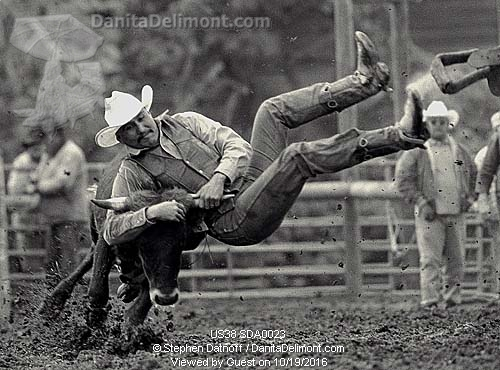
\includegraphics[width=.6\textwidth]{Wrangling2.jpg}
\end{center}
\caption{An illustration of a (metaphorical) datum being wrangled into submission.}
\end{figure}

\subsection{Some data wrangling principles} 
So you would like to a record of the data wrangling process (so that it 
is repeatable and even reversible), and automate it to the extent 
possible. To this end, here are some guidelines:

\begin{itemize}
	\item Store data in universally-readable, nonproprietary software formats (e.g., {\tt .csv})
	\item Use 
	plain ASCII text for your file names, variable/field/column names, and data 
	values --- make sure the ``text encoding'' is correct and standard 
	(e.g., {\tt UTF-8})
	\item Keep a metadata file for each unique dataset (agian, in 
	non-proprietary format)
	\item Don't (over-)modify your raw data by hand --- use scripts 
	instead --- keep a copy of the data as they were recorded.
	\item Use meaningful names for your data and files and field (column) names
	\item When you add data, try not to add columns (widening the format); rather, design your 
	tables/datasheets so that you add only rows (lengthening the format) 
	--- and convert ``wide format data'' to ``long format data'' using 
	scripts, not by hand!
	\item All cells within a data column should contain only one type of 
	information (i.e., either text (character), numeric, etc.). 
	\item Ultimately, consider creating a relational database for your 
	data (see the last section of this Chapter).
\end{itemize} 
This is not an exhaustive list either --- see the Borer et al (2009) 
paper in your readings list.

We will use the Pound Hill dataset collected by students in a past Silwood 
Field Course week for understanding/illustrating some of these 
principles. 

To start with, we need to import the {\tt raw} data file. 
\begin{compactitem}[$\quad\star$]
	\item Go to the bitbucket repository and navigate to the {\tt Data} 
	directory. 
	\item Copy the file {\tt PoundHillData.csv} and {\tt 
	PoundHillMetaData.csv} files into your own R module's {\tt
	Data} directory. 
	\item Now load the data in R: 
\end{compactitem}

\begin{lstlisting}
> MyData <- as.matrix(read.csv("../Data/PoundHillData.csv",header = F, 
stringsAsFactors = F))
> MyMetaData <- read.csv("../Data/PoundHillMetaData.csv",header = T, 
sep=";", stringsAsFactors = F)
\end{lstlisting}
Note that:
\begin{compactitem}
\item Loading the data {\tt as.matrix()}, and setting The {\tt header} 
and {\tt stringsAsFactors} guarantees that the data are imported "as 
is" so that you can wrangle them. Otherwise {\tt read.csv} will convert 
the first row to column headers, convert everything to factors, etc. 
Note that all the data will be converted to character class in matrix 
here because at least some of the entries are already character class.

\item For the metadata loading, the {\tt header} is set to true because 
we do have metadata headers ({\tt FieldName} and {\tt Description}), 
and I have used semicolon ({\tt ;}) as delimiter because there are 
commas in one of the field descriptions. 

\item I have avoided spaces in the columns headers (so ``FieldName'' 
instead of ``Field Name'') --- please avoid spaces in field or column 
names as much a possible as R will replace each space in a column 
header with a dot, which may be confusing.

\end{compactitem}

\begin{tipbox}
In {\tt R}, you can use {\tt F} and {\tt T} for boolean {\tt FALSE} 
and {\tt TRUE} respectively. Try:
\begin{lstlisting}
> a <- T
> a
[1] TRUE
\end{lstlisting}
\end{tipbox}

We won't do anything with the metadata file in this session except 
inspect the information it contains.   

\subsubsection{Keep a metadata file for each unique dataset} 

Data wrangling really begins immediately after data collection. You may 
collect data of different kinds (e.g., diversity, biomass, tree girth), 
etc. Keep the original spreadsheet well documented using a ``metadata'' 
file that describes the data (you would hopefully have written the 
first version of this even before you started collecting the data!). 
The minimum information needed to make a metadata file useful is a 
description of each of the {\it fields} --- the column or row headers 
under which the information is stored in your data/spreadsheet. Here is 
the metadata file for the Pound Hill dataset:
\begin{center}
	\begin{tabular}{|p{3.5cm} | p{11cm}|}
		\hline
		{\bf Field/Column Name} & {\bf Description} \\ \hline
		Cultivation	& Cultivation treatments applied in three months: october, may, march \\ \hline
		Block &	Treatment blocks ids: a--d \\ \hline
		Plot &	Plot ids under each treatment : 1--12 \\ \hline
		Quadrat	& Sampling quadrats (25$\times$50 cm each) per plot: Q1--Q6 
		\\ \hline
		Species	data & Number of individuals (count) per quadrat \\ \hline
	\end{tabular}
\end{center}

Ideally, you would also like to add more information about the data, 
such as the measurement units of each type of observation. Here, there 
is just one type of observation: Number of individuals of species per 
sample (plot), which is a count (integer, or {\tt int} class). 

\subsubsection{Don't (over-)modify your raw data by hand}

When the dataset is large (e.g., 1000's of rows), cleaning and 
exploring it can get tricky, and you are very likely to make many 
mistakes. You should record all the steps you used to process it with 
an R script rather than risking a manual and basically irreproducible 
processing. Most importantly {\it avoid or minimize editing your raw 
data file}. Let's see how we can modify the data using {\tt R}. In 
fact, we should now start to keep a record of what we are doing to the 
data. This is illustrated in a code data file available on the 
bitbucket repository. 

\begin{tipbox}
Sometimes you may run into (unexpected) bugs when importing and 
running scripts in {\tt R} because your file has a 
no-standard text encoding. You may need to specify the encoding in that 
case, using the {\tt encoding} argument of {\tt read.csv()} and {\tt 
read.table()}. You can check the encoding of a file by using {\tt find} in 
Linux/Mac. Try:
\begin{lstlisting}
$ file -i ../Data/PoundHillData.csv
\end{lstlisting}
or, check encoding of all files in the {\tt Data} directory: 
\begin{lstlisting}
$ file -i ../Data/*.csv 	
\end{lstlisting}
use {\tt file -I} instead of {\tt file -i} in a Mac terminal
\end{tipbox} 

\begin{compactitem}[$\quad\star$]
	\item Go to the bitbucket repository and navigate to the {\tt Code} 
	directory. 
	\item Copy the script {\tt DataWrang.R} into your own R module's {\tt 
	Code} directory and open it. 
\end{compactitem}

Go through the script carefully line by line, and make sure you 
understand what's going on. Read the comments --- add to them if you 
want. One of the examples of data modification that you must avoind 
doing by hand, is illustrated in the script: filling in zeros.  

\subsubsection{Convert wide format data to long format using scripts}

You typically record data in the field or experiments using a ``wide'' 
format, where a subject's (e.g., habitat, plot, treatment, species etc) 
repeated responses or observations (e.g., species count, biomass, etc) 
will be in a single row, and each response in a separate column. The 
raw Pound Hill data were recorded in precisely this way. However, the 
wide format is not ideal for data analysis --- instead you need the 
data in a ``long'' format, where each row is one observation point per 
subject. So each subject will have data in multiple rows. Any 
measures/variables/observations that don't change across the subjects 
will have the same value in all the rows.

\begin{tipbox}
For humans, the wide format is generally more intuitive for viewing and 
recording (e.g., in field data sheets) since one can actually view more 
of the data visually. However, the long format is more machine-readable 
and is closer to the formatting of databases. 
\end{tipbox}

You can switch between wide and formats using {\tt melt()} and {\tt 
dcast()} from the {\tt reshape2} package, as illustrated in {\tt DataWrang.R}. 

\subsection{And then came {\tt dplyr} and {\tt tidyr}}

So if you think this is the end of the options you have for data 
wrangling in R, think again. There are new kids on the block: {\tt dplyr} 
--- the next iteration of {\tt plyr} that addresses the speed issues in 
the latter, and {\tt tidyr}, essentially a nicer wrapper to the {\tt 
reshape2} package with additional functions. 
  
You will have to install these packages using {\tt sudo apt get 
install} in Linux or {\tt install.packages()} across all platforms (see 
Chapter \ref{chap:RI}). 

Together, these two packages have many many useful functions. Let's 
have a quick look at {\tt dplyr}:

\begin{lstlisting}
require(dplyr)
attach(iris)
dplyr::tbl_df(iris)	#like head(), but nicer!
dplyr::glimpse(iris) #like str(), but nicer!
utils::View(iris) #same as fix()!
dplyr::filter(iris, Sepal.Length > 7) #like subset(), but nicer!
dplyr::slice(iris, 10:15) # something new!
\end{lstlisting}

Note that the double colon ({\tt ::}) notation of {\tt dplyr} and {\tt 
tidyr} is like the dot notation in {\tt python} --- it allows you to 
access a particular function from these packages. So, for instance, if 
you want to use {\tt tbl\_df()} from {\tt dplyr}, the command syntax 
would be {\tt dplyr::tbl\_df(MyData)}. This new syntax is basically to 
avoid conflict in names of functions in by these new packages with the 
function names that already exist in the base R packages. For example, 
the {\tt dplyr} function {\tt filter} already exists in the base R 
package {\tt stats}. Thus, when you first load {dplyr}:  
\begin{lstlisting}	
> library(dplyr)
\end{lstlisting}	
you get:
\begin{lstlisting}	
Attaching package: 'dplyr'

The following objects are masked from 'package:stats':

    filter, lag

The following objects are masked from 'package:base':

    intersect, setdiff, setequal, union
\end{lstlisting}

Learning to use {\tt ddply} and {\tt tidyr} involves learning some new 
syntax and a lot of new commands, but if you plan to do a lot of data 
wrangling, you may want to get to know them well. Have a 
look at \url{https://blog.rstudio.org/2014/01/17/introducing-dplyr} and 
this cheatsheet: 
\url{https://www.rstudio.com/wp-content/uploads/2015/02/data-wrangling-cheatsheet.pdf}, also available in the Readings directory under {\tt DataDataData!} in 
the course bitbucket repository.

\subsection{On to data exploration}

Once you have wrangled the Pound Hill data to its long format, you are 
ready to go! You may want to start by examining the basic properties 
of the data, such as the number of tree species (41) in the dataset, 
number of quadrats (replicates) per plot and cultivation treatment, 
etc.

The first plot you can try is a histogram of abundances of species, 
grouped by different factors. For example, you can look at 
distributions of species' abundances grouped by {\tt Cultivation}). 

\section{Practicals}

{\bf (Extra Credit)} We used {\tt reshape2} in {\tt DataWrang.R} for 
wrangling that dataset. Write a new script called {\tt DataWrangTidy.R} 
that uses {\tt dplyr} and {\tt tidyr} for the same data wrangling 
steps. The best way to do this is to {\tt cp} {\tt DataWrang.R} and 
rename it {\tt DataWrangTidy.R}. Then systematically redo the script 
from start to end, looking for a function in {\tt dplyr} and {\tt 
tidyr} that does the same thing in each wrangling step. 

For example, to convert from wide to long format, instead of using {\tt 
melt()} (or {\tt dcast()}) from the {\tt reshape2} package, you can use  
{\tt gather()} from {\tt tidyr}.

Don't forget the cheatsheet: 
\url{https://www.rstudio.com/wp-content/uploads/2015/02/data-wrangling-cheatsheet.pdf} 
(also available in the Readings directory under {\tt DataDataData!} in 
the course bitbucket repository).

\section{Handling Big Data in R}

The  buzzword `Big Data' basically refers to datasets that have the 
following properties:
\begin{enumerate}

\item A dataset that does not fit into available RAM on one system 
(say, > 2 gigabytes). 
\item A dataset that has so many rows (when in it's long format --- see 
above sections) that it significantly slows down your analysis or 
simulation without vectorization (that is, when looping).	
\end{enumerate} 

Both these criteria are programming language- and computer 
hardware-dependent, of course. For example, a 32-bit OS can only handle 
$\textasciitilde$2 GB of RAM, so your computer screams ``Big Data!'' (slows down/hangs) 
every time you try to handle a dataset in that range. 

R reads data into RAM all at once when you using the {\tt read.table} 
(or its wrapper, {\tt read.csv()} --- maybe you have realized by now 
that {\tt read.csv()} is basically calling {\tt read.table()} with a 
particular set of options. That is, objects in R live in memory 
entirely, and big-ish data in RAM will cause R to choke. Python has 
similar problems, but you can circumvent these to an extent by using 
{\tt numpy} arrays (Chapter \ref{chap:pythonII}).

There are a few options (which you can combine, of course) if you 
are actually using datasets that are so large:

\begin{itemize}
	\item Import large files smartly; e.g., using {\tt scan()} in R, and 
	then create subsets of the data that you need. Also, use the {\tt 
	reshape} or {\tt tidyr} package to covert your data in the most 
	``square'' (so neither too long or too wide) format as possible. Of 
	course, you will need subsets of data in long format for analysis 
	(see sections above).
	\item use the {\tt bigmemory} package to load data in the gb range (e.g., use 
	{\tt read.big.matrix()} instead of {\tt read.table()}. This package 
	also has other useful functions, such as {\tt foreach()} instead of 
	{\tt for()} for better memory management. 
	\item Use a 64 bit version of R with enough memory and preferably on 
	Linux!
	\item Vectorize your analyses/simulations to the extent possible 
	(Chapters \ref{chap:pythonII}, \ref{chap:R_II}). 
	\item Use databases.
	\item use distributed computing (distribute the analysis/simulation 
	across multiple CPU's).
\end{itemize}
 
The next subsection superficially covers databases. We will cover 
memory management in the advanced Python, HPC and C weeks.

\subsection{Databases and R}

R can be used to link to and extract data from online databases such as PubMed 
and GenBank, or to manipulate and access your own. 
Computational Biology datasets are often quite 
large, and it makes sense to access their data by querying the 
databases instead of manually downloading them. So also, your own data 
may be complex and large, in which case you may want to organize and 
manage those data in a proper relational database. 

Practically all the data wrangling principles in the previous sections 
are a part and parcel of relational databases. 

There are many R packages 
that provide an interface to databases (SQLite, MySQL, Oracle, etc). 
Check out R packages {\tt DBI} 
(\url{http://cran.r-project.org/web/packages/DBI/index.html}) and {\tt 
RMySQL} 
(\url{https://cran.r-project.org/web/packages/RMySQL/index.html}.

And just like python (see Chapter \ref{chap:pythonII}), R can also be used 
to access, update and manage databases. In particular {\tt SQLite} 
allows you to build, manipulate, and access databases easily. Try this script 
(available in the {\tt Code} directory of the master repo):
\lstinputlisting[language=R]{Practicals/Code/SQLinR.R} 
This assumes that you are already familiar with the databases section 
of Chapter \ref{chap:pythonII}. 

\section{Practicals wrap-up}

  \begin{enumerate}

	\item Review and make sure you can run all the commands, code 
	fragments, and named scripts we have built till now and get the 
	expected outputs.

	\item Annotate/comment your code lines as much and as often as necessary 
	using \#.
	
	\item Keep all code, data and results files organized in you R 
	module directory
	 
   \end{enumerate}

\begin{center}
	\it {\tt git add}, {\tt commit} and {\tt push} all your code and data 
	from this chapter to your git repository.
\end{center}

\section{Readings}
Check out {\tt DataDataData!}, {\tt Visualization} and {\tt R} under 
{\tt Readings} on the bitbucket master repository
\begin{itemize}
   
  \item Brian McGill's ``Ten commandments for good data management''; \url{https://dynamicecology.wordpress.com/2016/08/22/ten-commandments-for-good-data-management/}

  \item This paper covers similar ground (look in your readings 
  directory): Borer, E. T., Seabloom, E. W., Jones, M. B., \& 
  Schildhauer, M. (2009). Some Simple Guidelines for Effective Data 
  Management. Bulletin of the Ecological Society of America, 90(2), 
  205--214.
  
  \item wrangler: \url{http://vis.stanford.edu/papers/wrangler}

  \item An interactive framework for data cleaning: \url{https://www2.eecs.berkeley.edu/Pubs/TechRpts/2000/CSD-00-1110.pdf}

  \item \url{http://www.theanalysisfactor.com/wide-and-long-data/}

	\item Rolandi et al. ``A Brief Guide to Designing Effective
	Figures for the Scientific Paper'', doi:10.1002/adma.201102518

	\item The classic Tufte \url{www.edwardtufte.com/tufte/books\_vdqi}

   Available in the Central Library, I have also added extracts and a 
    related book in pdf on the master repository

		(btw, check out what Tufte thinks of PowerPoint; \url{ https://www.edwardtufte.com/tufte/powerpoint})\\

	\item Lauren {\tt et al.} ``Graphs, Tables, and Figures in
	Scientific Publications: The Good, the Bad, and How Not to Be the
	Latter'', doi:10.1016/j.jhsa.2011.12.041

  \item Effective scientific illustrations: 
    \url{www.labtimes.org/labtimes/issues/lt2008/lt05/lt\_2008\_05\_52\_53.pdf} 

  \item 
    \url{https://web.archive.org/web/20120310121708/http://addictedtor.free.fr/graphiques/thumbs.php}

\end{itemize}

\chapter{High Performance Computing}
\label{chap:HPC}

This chapter introduces you to HPC in python using of the Imperial College HPC (\url{(https://wiki.imperial.ac.uk/display/HPC/Introduction}). 

\section{Local parallel processing}

Note that there are a number of ways in which you can develop HPC implementations for your code locally (on your own computer). I will not cover these, but here is a list of particularly useful approaches/tools:

\begin{itemize}
   \item Ipython {\tt parallel}: \url{https://ipython.org/ipython-doc/3/parallel/}
  \item Multi-threading, using the {\tt threading} package: \url{https://docs.python.org/3/library/threading.html}
  \item Using multiple processors with the {\tt multiprocessing} package    \url{https://docs.python.org/2/library/multiprocessing.html} 
\end{itemize}

The difference between threading and multiprocessing is that threads share in the same memory space, while processes have separate memory spaces. This makes it a harder to share information between processes with multiprocessing, but this is till a useful approach for quick and dirty parallelization. When better communication between processes is required, sophisticated solutions such as MPI and OpenMP may be needed. The MPI (Message Passing Interface) standard/protocol can be used in Python to parallelize your code over multiple processors through the {\tt mpi4py} package: \url{http://mpi4py.scipy.org/docs/usrman/index.html}. You can also parallelize numpy array loops with {\tt cython} and OpenMP: \url{http://www.perrygeo.com/parallelizing-numpy-array-loops-with-cython-and-mpi.html}.

\section{Running python scripts on IC HPC}

{\it These instructions also apply, with suitable modifications, for R 
scripts.}

\subsection{Preparing the scripts for running on the HPC}

The script you will run needs a sha-bang (telling it what shell to run, 
usually bash), you need to allocate resources to PBS (such as walltime, 
number of processors, and memory , using the {\tt \#PBS} directive), and tell it what Python script to run. The bash script could look something like this:

\lstinputlisting{Practicals/Code/PythonHPC.sh}

Or, you can do something like this to move all files one-by-one to 
avoid exceeding memory allocation ({\tt *.p} indicates that you used 
{\tt pickle} to dump results):

\begin{lstlisting}
for f in *.p; do
	echo "Processing $f..."
	mv $f $WORK/TestPyHPC/output/
done
\end{lstlisting}

NOTE: Most of the cx1 nodes have multiple cores, so there's no fixed memory assigned to each core. If you use more memory than your request on your {\tt \#PBS} directive, your job is likely to be terminated. If you request more memory than is available, the job will remain queued until sufficient memory is free for the job to run.

Your HPC enabled Python code could look like this:

\lstinputlisting{Practicals/Code/MyHPCScript.py}

Note the lines in this Python code where you  the environment so that it
knows the working directory and where to output files.

\subsection{Copying scripts from your computer to the HPC server}
 
Then, secure copy bash script file to {\tt \$HOME} on HPC server following
{\tt \$ scp source host:destination} structure, e.g.:

\begin{lstlisting}
$ scp script.sh user@login.cx1.hpc.ic.ac.uk:/home/user/whatever/script.sh
\end{lstlisting}

\subsection{Running the scripts}

Open a secure shell (ssh):

\begin{lstlisting}
$ ssh user@login.cx1.hpc.ic.ac.uk
\end{lstlisting}

where {\tt user} is your ICL username. You will then be prompted to enter your (ICL) password. Once on the HPC server, check for available modules:

\begin{lstlisting}
$ module avail
\end{lstlisting}

Your job then needs to be queued using {\tt qsub} (PBS):

\begin{lstlisting}
  $ qsub -j eo script.sh
\end{lstlisting}

where {\tt -j eo} is an option to join both output and error into one 
file. Running the script will produce a job output (anything that is 
printed in the shell terminal (e.g. {\tt echo})), and an error file 
(related to whether the script was successful or not), in the form of 
\{scriptname\}.o\{job id\} and \{scriptname\}.e\{jobid\}.\\

The {\tt qstat} command provides information on the job being submitted 
(which queue (short, medium, long), status, etc.) as well as 
information on all queues available (-q, -Q).

\subsection{Using a python script to submit jobs}
PBS also  allows  you  to  submit jobs using a Python (instead of 
shell) script. Look up the {\tt qsub} manual ({\tt man qsub}) in the 
HPC terminal, or visit 
\url{https://gist.github.com/nobias/5b2373258e595e5242d5}.

For example, the Python job script named  "MyHPCPy.py"  for  a  job  named  "HelloJob" prints "Hello":

\begin{lstlisting}
  #!/usr/bin/python
  #PBS -l select=1:ncpus=3:mem=1gb
  #PBS -N HelloJob
  print "Hello"
\end{lstlisting}

To run a Python job script you would do the same a for a bash job script above:

\begin{lstlisting}
$ qsub MyHPCPy.py
\end{lstlisting}

\section{Readings \& Resources}
\begin{itemize} \itemsep6pt
    \item IC library gives you with access to several e- and paper books on UNIX, some specific to Ubuntu. Browse or search and find a good intro book.
    \item The ICL HPC wiki is a very useful resource: \url{https://wiki.imperial.ac.uk/display/HPC/Command+line}
\end{itemize}



\chapter{The computing Miniproject}
\label{chap:miniproj}

%TODO
% Add to miniproject requirements/instructions:
% *Include justification in readme and main report why each scripting language was used
% * Indicate what each package is for in readme
% * Indicate version of each language used.

We have talked a lot about workflows and confronting models with data. 
It's time to do something concrete with all the stuff you have learnt!

This practical gives you an opportunity to try the ``whole nine yards'' 
of developing and implementing a workflow and delivering a ``finished 
product'' here you ask and answer a scientific question in biology 
(potentially involving multiple sub-questions/hypotheses). The 
miniproject will give you an opportunity to perform a ``dry run'' of 
executing your actual dissertation project.

\section {Objectives}

{\bf The main, generic question you will address is:} {\it What 
mathematical model best fits an empirical dataset?} 

You may think of this as testing a set of alternative hypotheses --- 
arguably every alternative hypothesis is nothing but an alternative model to 
describe an observed phenomenon. 
 
You may choose any dataset and set of alternative models, provided that 
the work can feasibly be done in the time you have for your miniproject 
(see the CMEE Guidebook for the submission deadline). You may choose a 
problem and dataset that is a related to, or even preliminary work for 
your main Masters project (to give you a reality/feasibility) check.  

The Miniproject must satisfy the following criteria:  
\begin{enumerate}
	
	\item It should employ all the biological computing tools you 
	have learned so far: shell (bash) scripting, git, \LaTeX, R, and 
	Python. Using these tools, you will build a workflow that starts with 
	the data and ends with a written report (in \LaTeX).
	
	\item {\it Atleast} two different models (hypotheses) must be fitted 
	to the data. The models should be fitted and selected using an 
	appropriate method (e.g., non-linear least squares for model fitting and 
	the Akaike Information Criterion for mdoel selection, respectively). 
	You will be given a primer on model fitting before you start on your 
	Miniproject. 
	
	\item The project should be fully reproducible --- a script should glue the 
	workflow together and run it. I should need to run just this script to get 
	everything to work, from data processing to model fitting to plotting 
	(e.g., in {\tt R}) to compilation of the \LaTeX written report.
	   
\end{enumerate}

If you are unable to find a dataset and/or problem that you would like 
to tackle, you may use the ``TPC problem'' given below.

\section{The Report}

	The report should,
	\begin{compactitem}
		\item be written in \LaTeX~ using the {\tt article} document class, 
		in 11pt (any font will do, within reason!)
	
		\item be double-spaced, with {\it continuous} line numbers 
	
		\item have a title, author name with affiliation and wordcount 
		(next point) on a separate title page.
		
		\item The report body itself should have an introduction with 
		objectives of the study, and appropriate additional 
		sections such as methods, data, results, discussion, etc. 
		
		\item must contain $\leq$3500 words {\it excluding the contents of 
		the title page and the references} --- there 
		should be a word count at the beginning of the document (I suggest using {\tt texcount}).
	
		\item all references should be properly cited using bibtex.
	
	\end{compactitem}

For the writeup, you probably should look at the {\it general} ( {\it 
not} word count, formatting etc.) dissertation writing guidelines given 
in the Silwood Masters Student Guidebook.  

\section{Patching together your workflow components}

Use Python and/or bash scripting for this. If using bash, call it  {\tt run\_MiniProject.sh} and if using Python, called it {\tt run\_MiniProject.py}. It should run all the 
components of the project's workflow, including compilation of 
the \LaTeX document. Look back at the notes to see how you would run 
these different components --- we have already covered how to run {\tt 
R} and compile \LaTeX using {\tt subprocess} in python.

\section{Submission}

Commit and push all your work to your bitbucket repository using a 
directory called {\tt CMEEMiniProject} at the same level as the {\tt 
Week1}, {\tt Week2} etc. directories, by the Miniproject deadline given 
in your CMEE course guidebook.

At this stage, I am not going to tell you how to organize your project 
--- that's one of my marking criteria (see next section). 

\subsection {Marking criteria}

I will be looking for the following while assessing your submission:

\begin{compactitem}

	\item A well-organized project where code, results, data, etc., are 
	easy to locate, inspect, and use 

	\item A python or bash script called {\tt run\_MiniProject.py} or {\tt 
	run\_MiniProject.sh} respectively, that runs the project

	\item A report that contains all the components indicated above in 
	``The Report'' subsection --- I will be looking for some 
	original thought and synthesis in the Intro and Discussion

	\item Quality of the presentation of the graphics and tables in your 
	report, as well as any plots showing model fits to the data.  

\end{compactitem}

Here again, the marking criteria you may refer to is the summative 
marking criteria given in Appendix \ref{chap:Appendices} titled 
``MARKING CRITERIA for EXAMS and ESSAYS and COURSEWORK''.  

{\it Equal weightage will be given to the code+workflow and writeup 
components --- each component will be marked to a max of 100 pts and then rescaled to a single mark / 100 using equal weightage}
 
\section {A Candidate Problem: Fitting TPCs}

One choice you have is to use a large dataset that we can provide to 
address the following question: {\it How well do different mechanistic models 
based upon biochemical principles vs. phenomenological principles fit on thermal responses of 
metabolic traits (rates)?}. This is actually part of the biotraits 
database that you were introduced to in the Python and Databases Section.  

This is currently a ``hot'' (no pun intended!) topic in biology, with 
both ecological and evolutionary consequences, as we discussed in the 
modelling lecture. On the {\it ecological side}, because the 
temperature-dependence of metabolic rate sets the rate of intrinsic 
$r_{max}$ (papers by Savage et al., Brown et al.) as well as 
interactions between species, it has a strong effect on population 
dynamics. In this context, note that 99.9\% of life on earth is 
ectothermic! On the {\it evolutionary side}, the temperature-dependence 
of fitness and species interactions also means that warmer environments 
may have stronger rates of evolution. This may be compounded by the 
fact that mutation rates may also increase with temperature (papers by 
Gillooly et al.).

\subsection{The Data}

The dataset is called {\tt GrowthRespPhotoData.csv} and contains 
hundreds of ``thermal responses'' for growth, respiration and 
photosynthesis rates in plants and bacteria (both aquatic and terrestrial). These were 
collected through lab experiments across the world, and compiled by 
various people over the years.

\subsection {The Models}

There are multiple models that might best describe these data.

The Schoolfield model (paper is in {\tt Readings} directory) is one
mechanistic option (\ref{fig:schoolf}) that is based upon 
thermodynamics and enzyme kinetics:

\begin{equation} \label{eq:schoolf}
	\begin{aligned}
	  B = \frac{B_0 e^{\frac{-E}{k} (\frac{1}{T} - \frac{1}{283.15})}}
    { 1 + e^{\frac{E_l}{k} (\frac{1}{T_l} - \frac{1}{T})} + 
    e^{\frac{E_h}{k} (\frac{1}{T_h} - \frac{1}{T})}}
	\end{aligned}
\end{equation}

Here, $k$ is the Boltzmann constant ($8.617 \times 10^{-5}$ eV $\cdot$ 
K$^{-1}$), $B$ the value of the trait at a given temperature $T$ (K) (K 
= $\degree$C + 273.15), while $B_0$  is the trait value at 283.15 K 
(10\degree C) which stands for the value of the  growth rate at low 
temperature and controls the vertical offset of the curve. $E_l$ is the 
enzyme's low-temperature de-activation energy (eV) which controls the 
behavior of the enzyme (and the curve) at very low temperatures, and 
$T_l$ is the at which the enzyme is  50\% low-temperature deactivated. 
$E_h$ is the enzyme's high-temperature de-activation energy (eV) which 
controls the behavior of the enzyme (and the curve) at very high 
temperatures, and $T_h$ is the at which the enzyme is  50\% 
high-temperature deactivated. $E$ is  the activation energy (eV) which 
controls the rise of the curve up to the peak in the ``normal operating 
range'' for the enzyme (below the peak of the curve and above $T_h$). 

\begin{figure}\label{fig:schoolf}
		\centering 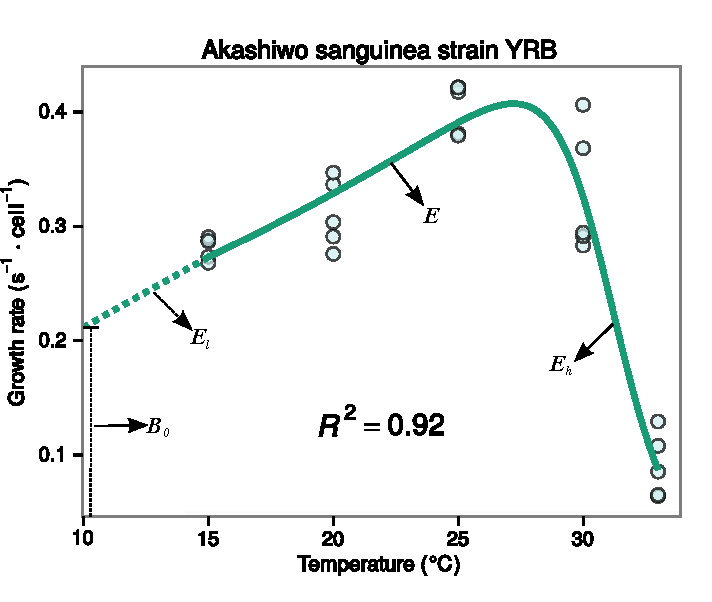
\includegraphics[width=.6\textwidth]{SchoolfEx.pdf} 
		\caption{Example of a unimodal thermal response curve for a 
		biological trait with the Schoolfield model fitted (Equation 
		\ref{eq:schoolf}).}
\end{figure}

In many cases, a simplified Schoolfield model would be more appropriate 
for thermal response data, because low temperature inactivation is 
weak, or is undetectable in the data because low-temperature 
measurements were not made.

\begin{equation} \label{eq:schoolfHi}
	\begin{aligned}
	  B = \frac{B_0 e^{\frac{-E}{k} (\frac{1}{T} - \frac{1}{283.15})}}
    { 1 +  e^{\frac{E_h}{k} (\frac{1}{T_h} - \frac{1}{T})}}
	\end{aligned}
\end{equation}

In other cases, a different simplified Schoolfield model would be more 
appropriate, because high temperature inactivation was not detectable 
in the data because measurements were not made at sufficiently high 
temperatures:

\begin{equation} \label{eq:schoolfLo}
	\begin{aligned}
	  B = \frac{B_0 e^{\frac{-E}{k} (\frac{1}{T} - \frac{1}{283.15})}}
    { 1 +  e^{\frac{E_l}{k} (\frac{1}{T_l} - \frac{1}{T})}}
	\end{aligned}
\end{equation}

In addition, there are phenomenological alternatives. These include the 
general cubic polynomial model:

\begin{equation}\label{eq:cubic}
	B = B_0 + B_1 T + B_2 T^2 + B_3 T^3
\end{equation}
with the parameters $B_0$, $B_1$, $B_2$ and $B_3$ not having any 
mechanistic underpinnings. Note that the cubic model has the same 
number of parameters as the the reduced Schoolfield model 
\ref{eq:schoolfH}. The parameter ($T$) of the cubic model (Equation 
\ref{eq:cubic}) are in $\degree$C.

{\it All the above parameters and equations are in SI units}.

\subsection {Fitting models to the data}

You will use Nonlinear Least Squares (NLLS) to fit the alternative 
models above (eqns \ref{eq:schoolf} -- \ref{eq:cubic}) to data, 
followed by model selection with AIC and BIC (also known as the 
Schwartz Criterion --- read the Johnson and Omland paper).
 
\subsection {The Workflow}

You will build a workflow that starts with the data and ends with a 
report written in \LaTeX. I suggest the following components and 
sequence in your workflow (you can choose to do it differently!):

\begin{enumerate}\itemsep0pt
	\item A Python or R script that imports the data and prepares it for 
	NLLS fitting, with the following features:
		\begin{compactitem}
			\item It should create unique ids so that you can identify unique 
			thermal responses (what does this mean?) 
			\item It should filter out datasets with less than 5 data points 
			(why?)
			\item It should deal with negative and zero trait values (why?) 
			\item The script should add columns containing starting values 
			of the model parameters for the NLLS fitting (how will you get 
			these?)
			\item Save the modified data to a new csv file. 
		\end{compactitem}
	\item A Python script that opens the new modified dataset (from 
	step 1) and does the NLLS fitting, with the following features:
			\begin{compactitem}
				\item Uses {\tt lmfit} --- look up submodules {\tt minimize}, 
				{\tt Parameters}, {\tt Parameter}, and {\tt report\_fit}.\\
				{\it Have a look through} 
				\url{http://lmfit.github.io/lmfit-py}, especially 
				\url{http://lmfit.github.io/lmfit-py/fitting.html#minimize}\\
				
				You will have to install lmfit using {\tt pip} or {\tt 
				easy\_install} - use {\tt sudo} mode.
				In addition to the lmfit example in class, you may want to look 
				for others online.
				
				\item Will use the {\tt try} construct because not all runs 
				will converge. Recall the {\tt try} example from R

				\item The more thermal response curves you are able to fit, the 
						better --- that is part of the challenge!

				\item Will calculate AIC, BIC, R$^{2}$, and other statistical 
				measures of fit (you decide what you want to include)
				
				\item Will export the results to a csv that the plotting R 
				script (next item) can read.

		\end{compactitem}

	\item A {\tt R} script that imports the results from the previous 
	step and plots every thermal response with both models (or none, if 
	nothing converges) overlaid --- all plots should be saved in a 
	single separate sub-directory. {\it Use {\tt ggplot} for pretty 
	results!} 

	\item \LaTeX~source code that generates your report.
	
	\item A Python script (saved in {\tt Code}) called {\tt 
	run\_MiniProject.py} that runs the whole project, right down to 
	compilation of the \LaTeX~ document. 

\end{enumerate}

Doing all this may seem a bit scary at the start. However, you need to 
approach the problem systematically and methodically, and you will be 
OK. I suggest the following to get you started:

\begin{compactitem}

	\item Explore the data in R and get a preliminary version of the 
	plotting script without the fitted models overlaid worked out. That 
	will also give you a feel for the data.

	\item Explore the two models -- be able to plot them. Write them as 
	functions in your {\tt python} script, because that's where you 
	will use them (step 2 above) (you can use {\tt matplotlib} for 
	quick and dirty plotting and then suppress those code lines later).

	\item Figure out, using a minimal example (say, with one, 
	"nice-looking" thermal response dataset) to see how the {\tt python}
	{\tt lmfit} module works. Kartik can help you work out the minimal
	example, including the usage of {\tt try} to catch errors in case the
	fitting doesn't converge. 
	
	\item One thing to note is that you will need to do the NLLS fitting 
	on the logarithm of the the function to facilitate convergence --- 
	please ask me or Sam Thompson if you need help on this.
	
\end{compactitem}

\section{Readings and Resources}

\begin{compactitem} \itemsep6pt
\item Levins, R. 1966 The strategy of model building in population 
biology. Am. Sci. 54, 421--431.  

\item Johnson, J. B. \& Omland, K. S. 2004 Model selection in ecology 
and evolution. Trends Ecol. Evol. 19, 101--108. 

\item For the suggested fitting TPCs project: Papers in the {\tt 
Temperature\_response\_papers} directory, but especially \\ 
Schoolfield, R. M., Sharpe, P. J. \& Magnuson, C. E. 1981 Non-linear 
regression of biological temperature-dependent rate models based on 
absolute reaction-rate theory. J. Theor. Biol. 88, 719--31. 

\end{compactitem}

% Appendix %%%%%%%%%%%%%%%%%%%%%%%%%%%%%%%%%%%%%%%%%%%%%%%%%%%%%%%
\begin{appendices} \appendixpage \noappendicestocpagenum \addappheadtotoc
{}
\chapter{Computing Coursework Assessment Criteria} \label{chap:Appendices}

Here is the marking scheme I will use:

	\begin{enumerate}
    \item You would get 100 pts if,
			\begin{enumerate}
				\item All the in-class scripts\footnote{{\it in-class scripts} are the ones that were give to you to practice with, which you only had to reproduce without error, while {\it assigned practicals / problems} are the assignments/problems you have been given that involve the writing of new scripts or the modification of existing ones. } were in place (in the code 
				directory in the respective week's directory) and functional 
				when run on my computer
        \item All the assigned practicals / problems are complete and functional, 
        and give the right answers.
        \item The scripts are all up to the the mark in terms of internal documentation and commenting
        \item There is a neat {\tt readme} file for the overall repository and in each of the weekly directories.
      \end{enumerate}

    \item For every in-class script that gives a syntax error, 5 pts deducted, and for every script that gives an error because of wrong path (e.g., absolute) assignment, 2 pts deducted.
    \item For every missing script or assigned practical/problem, 10 pts deducted
    \item For every assigned practical/problem, 5 pts deducted for 
    wrong answer if applicable (that is, script runs without error, but 
    gives wrong numerical or text output).
    \item For every missing {\tt readme} file, 1 pt deducted.
		\item For every extra, non-script file in {\tt Code} directory, 0.5 
		pt deducted.
		\item For every {\it valid} script file in {\tt Code} directory 
		lacking an appropriate extension, 0.5 pt deducted.
		\item For every result of a code/script run not saved to a separate directory, 1 pt deducted. For example, the separate directory may be {\tt Results} for new results, or {\tt Data}, if the scripts is for generating a new or modified dataset.   
    \item For every extra-credit question completed, 2.5 pts added.
	\end{enumerate}

From the points left after implementing the above criteria, I will 
exercise my judgement to deduct further marks if the weekly directory 
structure is disorganized, the code inadequately commented or 
insufficiently documented, or the written components of practicals are 
not up to the mark. 

You will get feedback if these issues needed to be addressed in the 
final written assessment. The final marks will be based upon these 
weekly points and a coursework marking criteria (See below). I will 
 up- or down-weigh the contribution of each week to the 
overall marks based upon the difficulty level. 

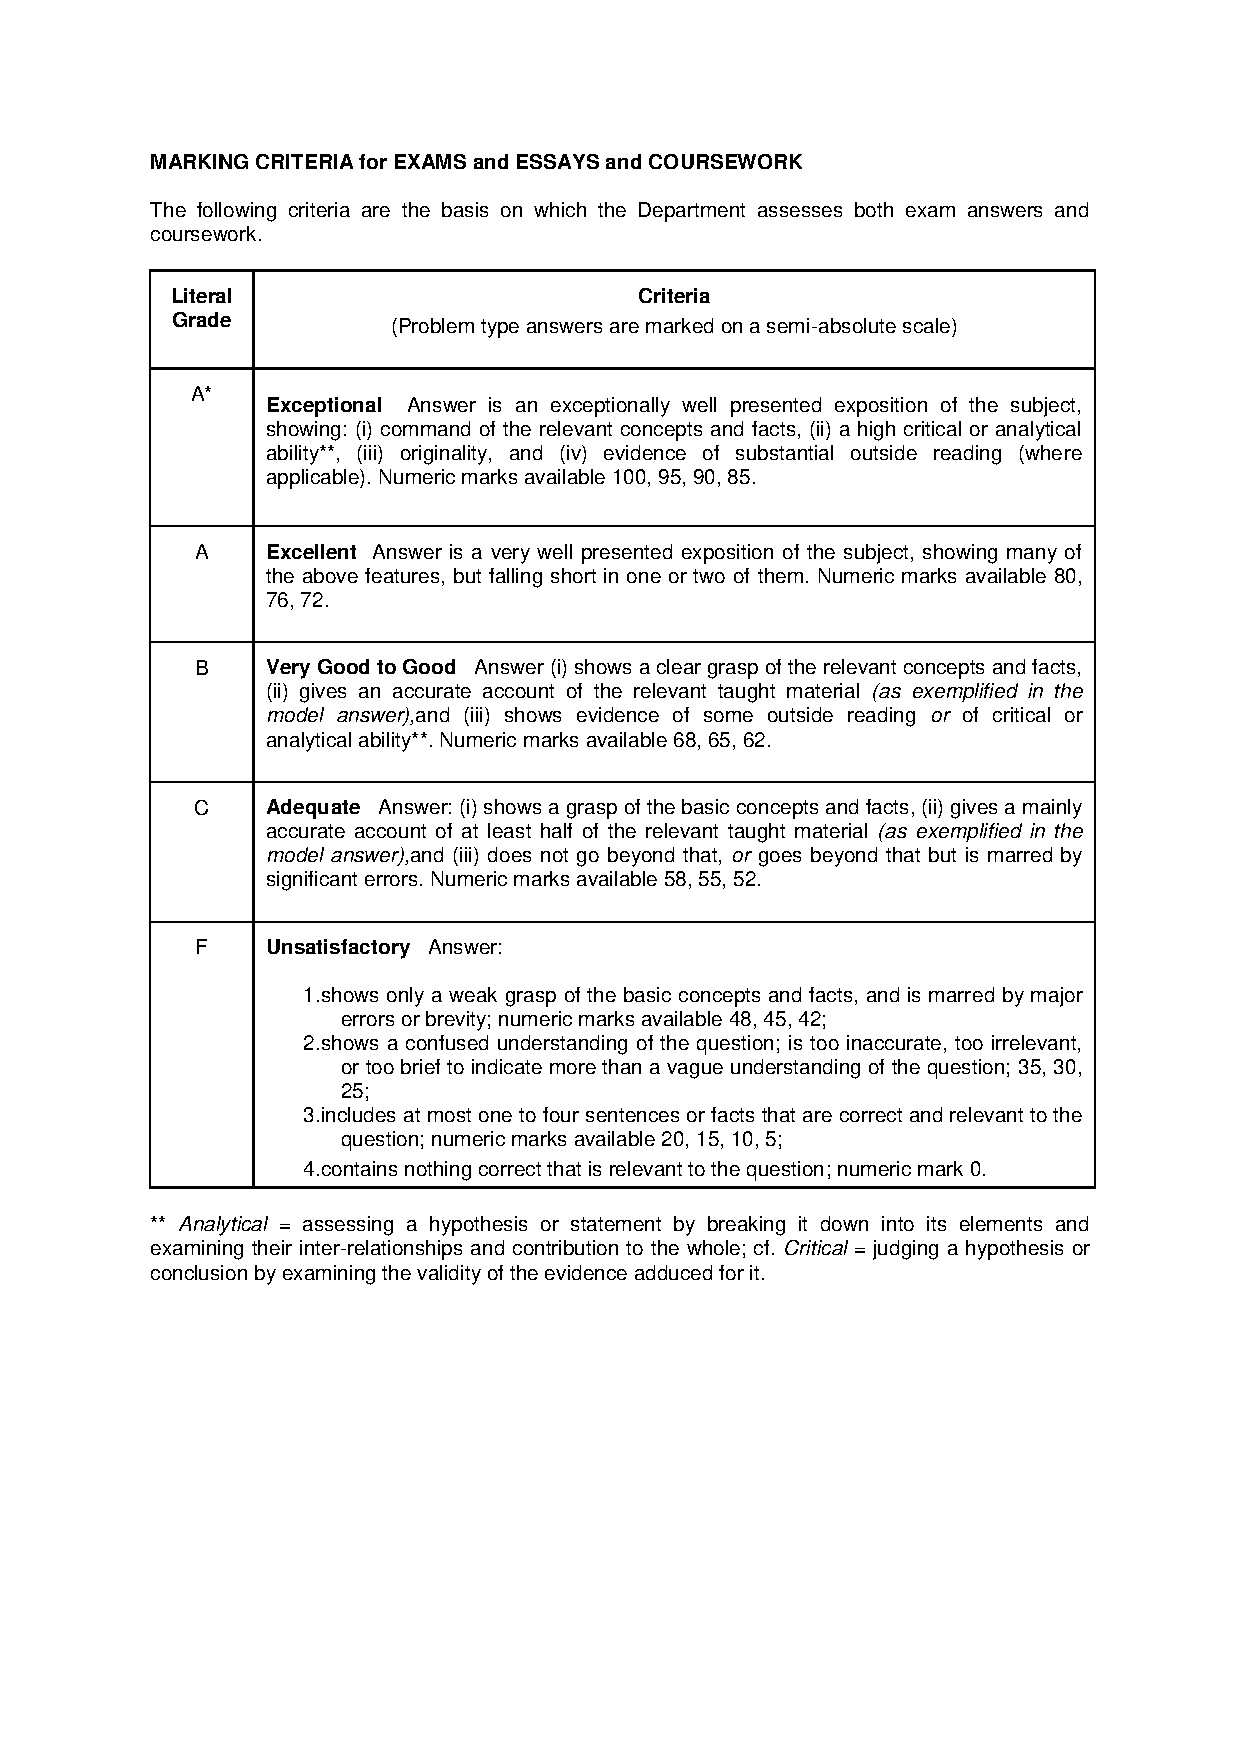
\includepdf[pagecommand={}]{MARKING_CRITERIA.pdf}
\end{appendices}


%%%%%%%%%%%%%%%%%%%%%%%%%%%%%%%%%%%%%%%%%%%%%%%%%%%%%%%
\backmatter 
\begin{figure}
	\begin{center}
	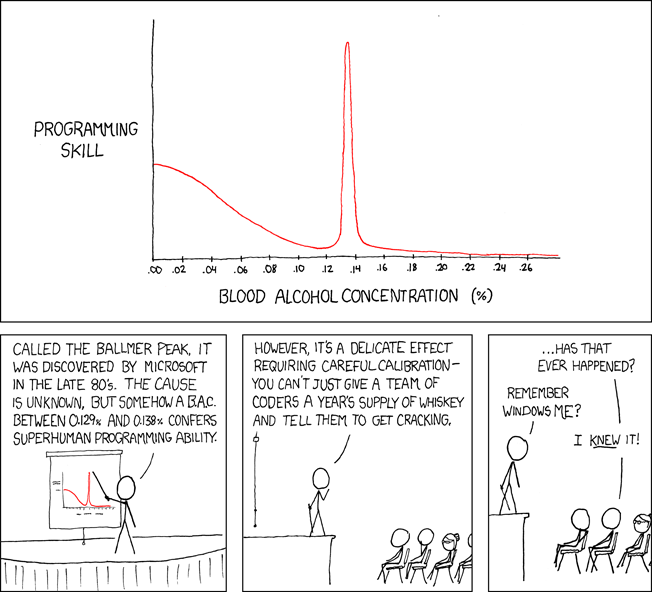
\includegraphics[width = 0.7 \linewidth]{ballmer_peak.png}\\
	\vspace{4pt}
	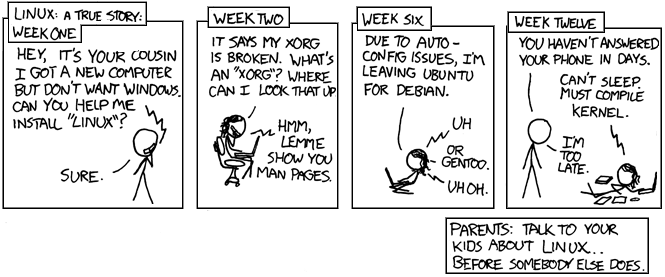
\includegraphics[width = 0.7 \linewidth]{cautionary.png}\\
	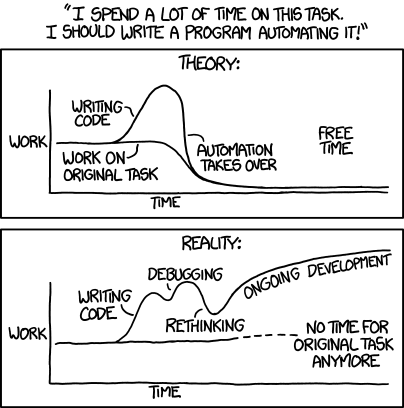
\includegraphics[width = 0.7 \linewidth]{automation.png}\\
	\url{www.xkcd.com}
	\end{center}
\end{figure}

%%%%%%%%%%%%%%%%%%%%%%%%%%%%%%%%%%%%%%%%%%%%%%%%%%%%%%%

\end{document}
